\documentclass[12pt,oneside]{uhthesis}
\usepackage{subfigure}
\usepackage[ruled,lined,linesnumbered,titlenumbered,algochapter,spanish,onelanguage]{algorithm2e}
\usepackage{amsmath}
\usepackage{amssymb}
\usepackage{amsbsy}
\usepackage{caption,booktabs}
\captionsetup{ justification = centering }
\captionsetup[table]{position=bottom}
% \usepackage{mathpazo}
\usepackage{float}
\setlength{\marginparwidth}{2cm}
\usepackage{todonotes}
\usepackage{listings}
\usepackage{xcolor}
\usepackage{multicol}
\usepackage{graphicx}
\floatstyle{plaintop}
\restylefloat{table}
\addbibresource{Bibliography.bib}
% \setlength{\parskip}{\baselineskip}%
\renewcommand{\tablename}{Tabla}
\renewcommand{\listalgorithmcfname}{Índice de Algoritmos}
%\dontprintsemicolon
\SetAlgoNoEnd

% \setcitestyle{square}
\definecolor{codegreen}{rgb}{0,0.6,0}
\definecolor{codegray}{rgb}{0.5,0.5,0.5}
\definecolor{codepurple}{rgb}{0.58,0,0.82}
\definecolor{backcolour}{rgb}{0.95,0.95,0.92}

\lstdefinestyle{mystyle}{
    backgroundcolor=\color{backcolour},   
    commentstyle=\color{codegreen},
    keywordstyle=\color{purple},
    numberstyle=\tiny\color{codegray},
    stringstyle=\color{codepurple},
    basicstyle=\ttfamily\footnotesize,
    breakatwhitespace=false,         
    breaklines=true,                 
    captionpos=b,                    
    keepspaces=true,                 
    numbers=left,                    
    numbersep=5pt,                  
    showspaces=false,                
    showstringspaces=false,
    showtabs=false,                  
    tabsize=4
}

\lstset{style=mystyle}

\title{Diseño de bases wavelets discretas basadas en la DST-II para detectar patrones en mamografías digitales}
\author{\\\vspace{0.25cm}Adrian Rodriguez Portales}
\advisor{\\\vspace{0.25cm}MSc. Damian Valdés Santiago}
\degree{Licenciado en Ciencia de la Computación}
\faculty{Facultad de Matemática y Computación}
\date{\\\vspace{0.25cm}\href{https://github.com/adrian13579/discrete-shapelet-transform}{github.com/adrian13579/discrete-shapelet-transform}}
\logo{Graphics/uhlogo}
\makenomenclature

\renewcommand{\vec}[1]{\boldsymbol{#1}}
\newcommand{\diff}[1]{\ensuremath{\mathrm{d}#1}}
\newcommand{\me}[1]{\mathrm{e}^{#1}}
\newcommand{\pf}{\mathfrak{p}}
\newcommand{\qf}{\mathfrak{q}}
%\newcommand{\kf}{\mathfrak{k}}
\newcommand{\kt}{\mathtt{k}}
\newcommand{\mf}{\mathfrak{m}}
\newcommand{\hf}{\mathfrak{h}}
\newcommand{\fac}{\mathrm{fac}}
\newcommand{\maxx}[1]{\max\left\{ #1 \right\} }
\newcommand{\minn}[1]{\min\left\{ #1 \right\} }
\newcommand{\lldpcf}{1.25}
\newcommand{\nnorm}[1]{\left\lvert #1 \right\rvert }
\renewcommand{\lstlistingname}{Ejemplo de código}
\renewcommand{\lstlistlistingname}{Ejemplos de código}

\begin{document}

\frontmatter
\maketitle

\begin{dedication}
	A mi familia, amigos y a todas las personas especiales que me acompañaron, por haber sido mi
	apoyo a lo largo de toda mi carrera universitaria y a lo largo de mi vida.
\end{dedication}

% \include{FrontMatter/Thanks}
\begin{opinion}
	La transformada wavelet se ha convertido en una de las técnicas más utilizadas para analizar las señales de audio e imágenes. Esta transformada se basa en funciones matemáticas especiales llamadas wavelets. La construcción de funciones wavelets es siempre un tema interesante y de gran aplicabilidad. Este es precisamente el tópico de esta tesis.

	En la literatura se reportan muchos enfoques de construcción que optimizan los parámetros matemáticos de dichas funciones como la regularidad, diferenciabilidad, momentos nulos, entre otras. Los métodos que permiten construir wavelets que sean capaces de reconocer en una señal determinados patrones definidos de antemano es menos frecuente. La creación de estas wavelets para patrones en 2 dimensiones (imágenes) no es tan frecuente en la literatura al respecto.

	La investigación realizada por el estudiante Adrian Rodriguez Portales se basa en la Transformada Shapelet Discreta II (DST-II) y propone tres alternativas de extensión 2D de dicha transformada. Para ello, primeramente, implementó la DST-II unidimensional y realizó experimentos para validar su eficiencia en la detección. Se compararon varios algoritmos para estimar la wavelet y se analizaron alternativas para su extensión a dos dimensiones. Se validó la propuesta en señales artificiales y en imágenes de mamografía digital. 

	Durante el desarrollo de la tesis Adrian estudió la literatura referente al análisis wavelet teórico de forma seria y crítica, proponiendo formas de cómputo de ciertas propiedades y parámetros involucrados en los algoritmos. Además, evaluó sus algoritmos en varias configuraciones experimentales (traslaciones, repeticiones del patrón, submuestreo del patrón) mostrando las ventajas y desventajas de este enfoque respecto a las wavelets clásicas. 

	Para esta tesis Adrian tuvo que estudiar las materias referidas, incluidas parcialmente en el currículo de la carrera, mostró disciplina, entrega y rigor. Además, demostró habilidades para el trabajo con la bibliografía y creatividad para proponer soluciones a problemas teórico-computacionales y de implementación, entre otras competencias de programación en el lenguaje Python y sus diversos frameworks. A pesar de que de las alternativas propuesta, solo uno mostró éxito en mamografía, considero que el estudiante logró cumplir exitosamente el objetivo propuesto y mostró que ciertos caminos no son adecuados para la extensión 2D de la DST-II, valor agregado de esta tesis.

	Por tanto, considero que a esta tesis del estudiante Adrian Rodriguez Portales debe otorgársele la máxima calificación (5 puntos, Excelente), y estoy seguro que en el futuro se desempeñará como un excelente profesional de la Ciencia de la Computación.

	\hspace*{\fill}\\
	\hspace*{\fill} MSc. Damian Valdés Santiago\\
    \hspace*{\fill} 26 de noviembre de 2022
\end{opinion}

\begin{resumen}
	La transformada de wavelet se ha convertido en una herramienta sumamente útil en el campo de procesamiento
	de señales. Sin embargo, la gran variedad de wavelets existente hace que la búsqueda de la mejor para 
	un problema determinado sea un proceso bastante complejo. En los últimos años, se han desarrollado
	técnicas para construir wavelets
	adaptadas a los datos. Una de estas técnicas es la Transformada Shapelet Discreta , que
	permite la construcción de una wavelet (llamada \textit{shapelet}) capaz de detectar patrones a partir de los cuales
	se construyó. Este método presenta algunas ventajas con respecto a los algoritmos de aprendizaje automático 
	usados en el estado del 
	arte para la detección y reconocimiento de patrones, pues no es necesario un gran volumen de datos. Sin embargo,
	existen muy pocos trabajos sobre dicho algoritmo, y solo ha sido evaluado en señales unidimensionales, hasta 
	donde el autor conoce. En este
	trabajo se explora precisamente su extensión al caso de imágenes. Se proponen varias alternativas para su aplicación
	al caso señales de dos dimensiones y se evalúan los resultados en imágenes artificiales y en la detección de masas en mamografías.
\end{resumen}

\begin{abstract}
	The wavelet transform has become an extremely useful tool
	in the field of signal processing. However, the great variety of wavelets
	existing makes finding the best one for a given problem
	quite a complex process. In recent years, techniques to build 
	adapted wavelet to the data have been developed. One of these techniques is the 
	Discrete Shapelet Transform, which allows the construction of a wavelet (called \textit{shapelet})
	able to detect patterns from which it was built. This method presents
	some advantages with respect to machine learning algorithms used in the state-of-the-art 
	for the detection and recognition of patterns, since it is not necessary a large volume
	of data. However, there are very few works on this algorithm, and it has only
	been evaluated on one-dimensional signals, according to the reviewed literature. 
	This paper explores precisely
	its extension to the case of images. Some alternatives are proposed for their application to the case of
	two-dimensional signals and the results are evaluated in artificial images, and in the
	detection of masses in mammogramphies.
\end{abstract}

\tableofcontents
\listoffigures
\listoftables
% \listofalgorithms
% \lstlistoflistings


\mainmatter

\chapter*{Introducción}\label{chapter:introduction}
\addcontentsline{toc}{chapter}{Introducción}

Muchos procesos de la naturaleza se pueden modelar como señales. El sonido, la luz y la actividad
cerebral de una persona son todos fenómenos que se representan a través de señales. Cada una con
sus características únicas. Esto ha motivado el estudio y la creación de herramientas capaces
de descubrir los secretos de las mismas. 

En 1822, Joseph Fourier publica su \textit{ Théorie analytique de la chaleur } \cite{Fourier2009} donde introduce la idea de usar
series matemáticas para analizar la conducción del calor en cuerpos sólidos. Esta teoría se conoce en
la actualidad como Teoría de Fourier. En la misma, se plantea que una señal se puede representar como
una serie, posiblemente infinita, de senos y cosenos. Este enfoque permite estudiar las diferentes 
frecuencias presentes en una señal y la amplitud de las ondas que la conforman. A la herramienta que permite
analizar el comportamiento de una función en el dominio de la frecuencia se le conoce en la actualidad como
Transformada de Fourier.

Las propiedades de esta transformada, la convierten en una herramienta muy poderosa para muchos escenarios. 
Sin embargo, su principal desventaja es que cuando se pasa al dominio de las frecuencias, la información 
temporal se pierde. La información de la frecuencia es fija en relación con el tiempo en una función 
trigonométrica. Esto es el caso contrario al de muchas señales, como el sonido, donde las características
cambian a lo largo del tiempo. 

En 1910 , Alfréd Haar introduce en su trabajo \textit{Zur Theorie der orthogonalen Funktionensysteme} \cite{Haar1910} un tipo 
funciones que en la actualidad se conocen como wavelets, pero no es
después de varias décadas que se les acuña este nombre. Estas funciones son como pequeñas ondas y a diferencia
de las funciones trigonométricas, son de pequeña duración y localizadas en tiempo permitiendo obtener información tanto temporal como
de frecuencia. Otra ventaja con respecto a la bases de Fourier, es que las bases wavelets no son únicas: 
existen una amplia variedad, para todo tipo de aplicaciones. 

La propagación de las wavelets en la comunidad científica y académica es sorprendente.
El surgimiento y consolidación de esta teoría a mediados de los 1980s, su conexión con el procesamiento
de señales y bancos de filtros \cite{Mallat2008}, el diseño de una algoritmo eficiente para el cómputo de la transformada \cite{Mallat2008}
y los aportes sobre el estudio de wavelet ortogonales \cite{daubechies1992} son algunos hechos que marcan su rápido desarrollo en
pocos años.   

Dejando un lado el aspecto puramente matemático, las wavelets también han tenido un gran impacto  
en muchos campos y problemas. Por ejemplo, el algoritmo de compresión de imágenes JPEG 2000 está basado en
bases wavelets \cite{Taubman2002}.

En el campo de la medicina las wavelets también han hecho una incursión bastante importante. Trabajos como
\cite{Bhattacharyya2018} y \cite{Sharma2020} muestran su aplicación en la detección de patrones y áreas de interés
en electroencefalogramas (EEG) respectivamente. Estudios como \cite{Too2018} han hecho una comparación de las distintos
tipos de wavelets en los EEG. 

En el procesamiento de imágenes médicas también han sido 
usadas en los útimos años, por ejemplo, en la compresión \cite{Bruylants2015}\cite{Alkinani2021}, en la eliminación de ruido
 \cite{Wang2006}\cite{George2016}\cite{Patil2021} y para 
mejorar el contraste \cite{Dikshit2022}.

Las wavelets también han evolucionado y han sido la base para nuevos algoritmos que añaden nuevas capacidades.
Tal es el caso de transformada discreta de \textit{shapelet} (DST) \cite{Guido2008} que está basada en la transformada discreta
de wavelet (DWT), pero que añade información de forma en conjunto con el clásico análisis temporal y de frecuencia de la
DWT. En un segundo trabajo se crea una segunda versión de este algoritmo, DST-II \cite{Guido2018}, y en \cite{Guido2021} se hacen 
algunas modificacones para obtener simetría, creando una tercera versión conocida como DST-III.
La DST, aunque poco estudiada, por sus propiedades de detección puede se una alternativa a otros algoritmos de
detección de patrones usados en el estado del arte que están basados en \textit{machine learning} y que requieren
de muchos datos para us correcto funcionamiento.

En la Facultad de Matemática y Computación, también se trabaja con las wavelets y su transformada, sobretodo en
investigaciones sobre el procesamiento de imágenes biomédicas. Las mamografías son uno de los tipos de imágenes
con las que se trabaja en este centro. 
Con la aparición del algoritmo de la DST-II, surge  
una alternativa que posee ciertas ventajas con otros enfoques  
usados en los últimos años para problemas de detección. Sin embargo, su uso solo ha sido estudiado para el 
caso de señales unidimensionales, por lo que es de interés para el centro experimentar y explorar su extensión
para el caso de señales bidimensionales. Por este motivo y partiendo de la hipótesis de que la DST se 
puede extender para el caso bidimensional y aplicar para la detección de patrones en mamografías, este trabajo tiene como 
objetivo general explorar el uso de la DST-II para detectar masas en mamografías. Para ello, se deben cumplir los 
siguientes objetivos específicos:

\begin{itemize}
	\item Revisión del estado del arte sobre la construcción de wavelets adaptadas 
	\item Evaluación numérica de algoritmos de optimización para estimar la \textit{wavelet}(\textit{shapelet})
		usando la metodología propuesta en la DST-II. En el artículo \cite{Guido2018} no se muestra
		cuál algoritmo numérico es utilizado para resolver el sistema de ecuaciones no lineales, 
		por lo cual este es un punto importante en la presente investigación.
	\item Replicación de la DST-II en el caso de señales y patrones unidimensionales. 
	\item Explorar ideas para la extensión de la DST-II para el caso bidimensional. 
	\item Aplicación del algoritmo en mamografías para la detección de masas y evaluación de los resultados.  
	\item Implementación de un software (interfaz gráfica) para el uso del algoritmo propuesto.
\end{itemize}

\section{Estructura del documento}

\chapter{Construcción de wavelets}\label{chapter:state-of-the-art}

El objetivo de este trabajo es replicar la DST-II y explorar su comportamiento en el caso de señales de dos 
dimensiones. Sin embargo, antes de hablar de los detalles de este algoritmo, es necesario introducir
algunos conceptos sobre las wavelets y su construcción. En la Sección \ref{wavelet-transform} 
de este capítulo se introducen la definición de wavelet
y de la transformada, tanto continua como discreta y la relación de esta última con los bancos de filtros. Luego, en
la Sección \ref{design-selection-wavelets} se exponen algunos 
de los criterios más usados para caracterizar a las wavelets y ejemplos de wavelets clásicas, para después 
hablar de algunas de las técnicas más recientes usadas en la generación de wavelets adaptadas a datos o problemas
específicos (entre ellas, la DST en sus tres variantes).

\section{Transformada Wavelet Continua }\label{wavelet-transform}

Antes de definir formalmente qué es una wavelet, es necesario definir el espacio de las funciones 
de cuadrado integrable.
Este espacio, denotado por $L^2(\mathbb{R})$ está formado por las funciones $f$ que cumplen \cite{frazier}:

\begin{equation}
	\int_{\mathbb{R}} |f(x)|^2 dx < \infty.
\end{equation}

Sobre este espacio, el producto interno $\langle \cdot,\cdot \rangle$ de $f,g \in L^2(\mathbb{R})$ se define como:
\begin{equation}
	\langle f,g \rangle = \int_{\mathbb{R}} f(x)g^*(x) dx,
\end{equation}
\noindent donde el operador $*$ denota el conjugado complejo.

Una wavelet es una función $\psi \in L^2(\mathbb{R})$ con promedio cero \cite{Mallat2008}:
\begin{equation}
	\int_{-\infty}^{+\infty} \psi(t) dt = 0.
\end{equation}
También se cumple que $\psi$ está normalizada, es decir, $||\psi||=1$. Además, $\psi$ está centrada en la vecindad
$t=0$. A partir de las traslaciones y dilataciones de $\psi$ se puede generar una familia de funciones:

\begin{equation}
	\left\{ \psi_{u,s}(t)= \frac{1}{\sqrt{s}}\psi \left(\frac{t-u}{s}\right) \right\}_{u \in \mathbb{R}, s \in \mathbb{R^+}},
\end{equation}
\noindent donde $u$ es el factor del desplazamiento y $s$ la escala. Estas nuevas funciones $\psi_{u,s}$ siguen estando
normalizadas. Luego, la transformada wavelet continua (TWC) de una función $f$ se define como:

\begin{equation}
	Wf(u,s) = \langle f,\psi_{u,s} \rangle = \int_{-\infty}^{+\infty}  f(t)\frac{1}{\sqrt{s}}\psi^*\left(\frac{t-u}{s}\right) dt.
\end{equation}

Si se define la operación de convolución como:
\begin{equation}
	f*g(x) = \int_{\mathbb{R}} f(x-y)g(x)dy,
\end{equation}
\noindent la TWC también se puede definir de esta forma:

\begin{equation}
	Wf(u,s) = \int_{-\infty}^{+\infty}  f(t)\frac{1}{\sqrt{s}}\psi^*\left(\frac{t-u}{s}\right) dt = f*\bar \psi_s(u),
\end{equation}
\noindent donde $$\bar \psi_s(t)=\frac{1}{\sqrt{s}}\psi^*\left(\frac{-t}{s}\right).$$

El concepto de función de escala también es importante cuando se trata de la transformada wavelet. 
Cuando $Wf(u,s)$ es conocido solamente para valores de $s<s_0$, para recuperar $f$ se necesita información
complementaria correspondiente a $Wf(u,s)$ para $s>s_0$. Por este motivo, se introduce
la función $\phi$, la cual se conoce como la función de escala, porque es la suma de todas las wavelets con
escalas mayores que uno. La función $\phi$ también está normalizada ($||\phi||=1$).

Sea 
\begin{equation}
	\phi_s(t) = \frac{1}{\sqrt{s}}\phi\left(\frac{t}{s}\right),
\end{equation}
\noindent entonces la aproximación de bajas frecuencias de $f$ se define como:

\begin{equation}
	Lf(u,s) = \langle f(t),\frac{1}{\sqrt{s}}\phi\left(\frac{t-u}{s}\right) \rangle = f*\phi_s(u).
\end{equation}


\subsection{Transformada Wavelet Discreta }

Para el caso de las señales discretas, una base wavelet discreta es necesaria. Por esto, primero se requiere
obtener un conjunto discreto de wavelets mediante la discretización de $s$ y $u$. Sea $u=ks$ y $s=a^j$, 
para $k,j \in \mathbb{Z}$ y $a>1$, entonces:

\begin{equation}
	\psi_j[n] = \frac{1}{a^j}\psi\left(\frac{n}{a^j}\right).
\end{equation}

Luego la transformada wavelet discreta (TWD) se define como \cite{Mallat2008}:

\begin{equation}\label{eq:Wf}
	Wf[n,a^j] = \sum_{m=0}^{N-1} f[m] \psi_{j}^*[m-n] = f * \bar \psi_j[n],
\end{equation}

\noindent donde $\bar \psi_j[n] = \psi_j^*[-n]$.

De forma similar, la función de escala se puede definir como:

\begin{equation}
	\phi_j[n] = \frac{1}{a^j}\phi\left(\frac{n}{a^j}\right),
\end{equation}

donde $\bar \phi_j[n] = \phi_j^*[-n]$. Luego, 

\begin{equation}\label{eq:Lf}
	Lf[n,a^j] = \sum_{m=0}^{N-1} f[m] \phi_{j}^*[m-n] = f \circledast \bar \phi_j[n],
\end{equation}

\noindent es una aproximación de $f$, pero sin los componentes de alta frecuencia, tal y como ocurría en el caso
de la TWC. 
Cuando $a=2$, se le conoce como transformada diádica \cite{Mallat2008}.

\subsection{Bancos de filtros}\label{filter-banks}

El uso de filtros en el procesamiento de señales es bastante amplio e incluso es anterior a 
la gran incursión de las wavelets en esta área. 
Sin embargo, ambos están relacionados y la TWD se puede definir en términos de filtros.

Un filtro es un operador lineal invariante en el tiempo. Actúa sobre un vector de entrada $x$.
El vector de salida $y$  es la convolución de $x$ con un vector fijo $h$, tal y como se muestra
a continuación \cite{Gilbert95} :

\begin{equation}
	y[n] = \sum_{k} h[k]x[n-k] = h * x.
\end{equation}

El vector $h$ contiene los coeficientes del filtro. En el caso de los filtros digitales, los 
coeficientes $h(n)$ vienen en tiempos discretos $t=nT$, donde $T$ es el período de muestreo. 
Si la entrada es un vector $x=(\cdots,0,1,0,\cdots)$, donde tiene una unidad de impulso en el tiempo cero,
es decir, $x[n-k]=0$, para $n \neq k$, entonces la suma de la convolución tiene un solo término, que sería
$h[n]$. Esta salida $y[n]=h[n]$, es la respuesta en el tiempo $n$ a la unidad de impulso
$x[0]=1$. La respuesta de impulso del filtro es $h[0],h[1],\cdots,h[N]$ \cite{Gilbert95}.

Si la respuesta de impulso del filtro es de duración finita, porque se hace cero en tiempo finito, entonces
el filtro se conoce como filtro de respuesta finita al impulso (FIR, en inglés).

En el dominio de las frecuencias, la convolución con el vector $h$, se convierte en una multiplicación. La 
acción de los filtros en el tiempo y la frecuencia son los fundamentos sobre los que el procesamiento de señales
está construido \cite{Gilbert95}.

Un banco de filtros es un conjunto de filtros. El banco de análisis, por lo general, tiene dos filtros, 
de paso bajo (\textit{lowpass}) y de paso alto (\textit{highpass}). Estos separan la señal 
de entrada en bandas de frecuencias. Normalmente, no es necesario
conservar la salida entera de los filtros de análisis y solamente se mantienen los componentes pares de la salida
de los filtros. Este proceso se llama submuestreo o decimación (\textit{downsampling}). 

En el marco de las wavelets ortogonales, el algoritmo de descomposición y reconstrucción se puede definir
en términos de operaciones con filtros. Las siguientes ecuaciones \cite{Mallat2008}:

\begin{equation}
	a_j[n] = \langle f,\phi_{j,n} \rangle,
\end{equation}

\begin{equation}
	d_j[n] = \langle f,\psi_{j,n} \rangle,
\end{equation}

\noindent son las proyecciones de $f$ sobre $\{\phi_{j,n}\}_{n\in \mathbb{Z}}$ y $\{\psi_{j,n}\}_{n\in \mathbb{Z}}$, 
respectivamente. El primer vector $a$ representa los coeficientes de aproximación de la función $f$,
y $d$ los de detalle. Estos coeficientes $d_j$ y $a_j$ corresponden a (\ref{eq:Wf}) y (\ref{eq:Lf}) 
respectivamente. 

Sean los filtros 

\begin{equation}
	h[n] = \langle \frac{1}{\sqrt{2}} \phi\left(\frac{t}{n}\right), \phi(t-n) \rangle,
\end{equation}

\begin{equation}
	g[n] = \langle \frac{1}{\sqrt{2}} \psi\left(\frac{t}{n}\right), \phi(t-n) \rangle,
\end{equation}

\noindent o de forma equivalente,

\begin{equation}
	\phi(t) = \sum_n \sqrt{2}h[n]\phi(2t-n),
\end{equation}

\begin{equation}
	\psi(t) = \sum_n \sqrt{2}g[n]\phi(2t-n).
\end{equation}

Las siguientes fórmulas muestran como calcular los coeficientes de la TWD, partiendo de los filtros 
$h$ y $g$, y es conocido como algoritmo de Mallat:

\begin{equation}\label{eq:mallat-aprox}
	a_{j+1}[p] = \sum_{-\infty}^{+\infty} h[n-2p]a_j[n] = (a_j * \bar h)[2p],
\end{equation}

\begin{equation}\label{eq:mallat-details}
	d_{j+1}[p] = \sum_{-\infty}^{+\infty} g[n-2p]d_j[n] = (d_j * \bar g)[2p],
\end{equation}

\noindent donde el operador $\bar x$ sobre $h$ y $g$ indican el reverso del filtro.

Las fórmulas (\ref{eq:mallat-aprox}) y (\ref{eq:mallat-details}) corresponden al banco de filtro para la
descomposición o análisis de la señal. 

En el caso del banco de filtro para el proceso inverso, es decir, la reconstrucción o síntesis de la señal a 
partir de los coeficientes, se tiene la siguiente fórmula:

\begin{equation}
	a_j[p] = \sum_{n= -\infty}^{+\infty} h[p-2n]a_{j+1}[n] + \sum_{n= -\infty}^{+\infty}g[p-2n]d_{j+1}[n],
\end{equation}

\noindent o de forma equivalente, 

\begin{equation}
	a_j[p] = ( \check a_{j+1} * h )[p] + ( \check d_{j+1} * g )[p],
\end{equation}

\noindent donde el operador $\check x$ sobre $a_j$ y $d_j$ denota la señal insertando ceros en los índices impares
(\textit{upsampled}).

\begin{figure}\label{fig:dwt-filterbanks-1D}
	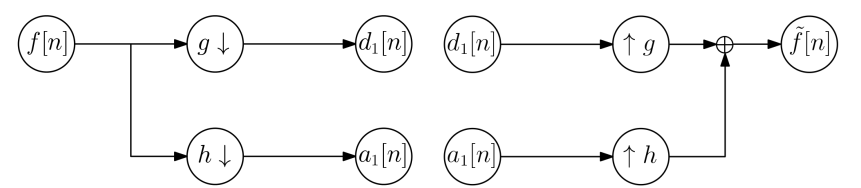
\includegraphics[scale=0.5]{Graphics/dwt-filterbanks-1D.png}
	\caption{Representación gráfica del proceso de descomposición (análisis) y reconstrucción (síntesis) de la señal $f$. La $\uparrow$ corresponde a la operación de \textit{upsampling} y la $\downarrow$ a la de \textit{downsampling} (Tomado de \cite{Recoskie2018} pág. 25).}\label{fig:dwt-filterbanks-1D}
\end{figure}

La Figura \ref{fig:dwt-filterbanks-1D} muestra una representación gráfica de ambos bancos de filtros, es decir, 
el proceso cómputo de la transformada y de su inversa. Empezando por $a_0[n] = f[n]$, se procede a calcular recursivamente
los coeficientes de aproximación y de detalle, tal y como se describe en (\ref{eq:mallat-aprox}) y (\ref{eq:mallat-details}),
respectivamente. Este algoritmo es bastante eficiente, pues tiene un costo computacional de $O(n)$, donde $n$
es el tamaño de la señal. 

Una de las propiedades de este algoritmo es la invertibilidad, es decir, después de haber sido deconstruída, el proceso
de reconstrucción permite obtener la señal original. La principal propiedad necesaria en un banco de filtro 
para que se cumpla lo anterior es la propiedad de reconstrucción perfecta. 

\subsection{TWD para dos dimensiones}\label{section:dwt-2d}

La transformada wavelet discreta se puede extender de varias formas para el caso de imágenes.
En la descomposición estándar la transformada es aplicada a todas las columnas para todas las escalas
y luego a todas las filas del resultado. En la descomposición no estándar la transformada se calcula en cada
eje por separado, es decir, primero se realiza la transformada a las filas y luego a las columnas del resultado. 
Esta forma de descomposición es la más usada y se denomina producto tensorial \cite{WaveletVariants2D}.

En el caso 1D, se calculan dos compenentes de la señal en cada iteración del algoritmo (paso alto y
paso bajo). En el caso 2D, para la descomposición no estándar, se calculan cuatro componentes. $LR$ y $LC$ son 
el resultado del filtro de paso bajo
sobre las filas y las columnas, respectivamente. De forma similar, se definen $HR$ y $HC$, pero para el caso
del filtro de paso alto. En cada iteración del algoritmo de la TWD, se obtienen las siguientes componentes:

\begin{itemize}
	\item Coeficientes de aproximación LL: $LC(LR(X))$
	\item Coeficientes de detalle horizontal LH: $LC(HR(X))$
	\item Coeficientes de detalle vertical HL: $HC(LR(X))$ 
	\item Coeficientes de detalle diagonal HH: $HC(HR(X))$
\end{itemize}

\begin{figure}
	\begin{center}
		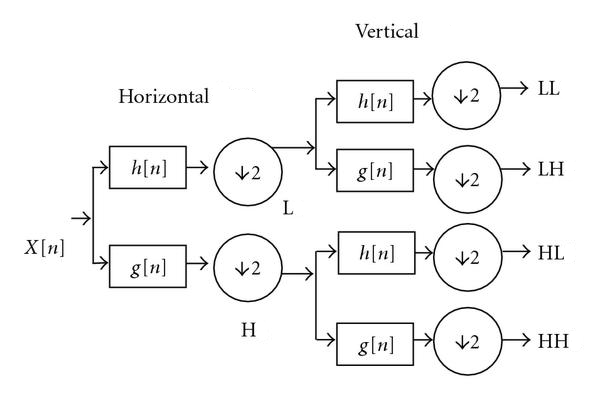
\includegraphics[scale=2]{Graphics/dwt-2D.png}
		\caption{Representación gráfica del proceso de descomposición (análisis) de la señal bidimensional $X$. La $\downarrow$ corresponde a la operación de \textit{downsampling}.}\label{fig:dwt-2D}
	\end{center}
\end{figure}

\noindent donde $X$ es una señal discreta de dos dimensiones. Los tres componentes calculados haciendo uso del 
filtro de paso alto son considerados coeficientes de detalle, y el otro restante, corresponde a los coeficientes de aproximación. 
Los grupos de coeficientes de
detalles, corresponden cada uno a una orientación: horizontal, vertical y diagonal. Cada uno responde a cambios en su
respectiva dirección. Al igual que en el caso unidimensional, se hace un submuestreo sobre la señal original
en cada convolución con los filtros. La Figura \ref{fig:dwt-2D} representa gráficamente
el proceso de obtención de la TWD para el caso de una señal bidimensional.

En el aspecto de la complejidad computacional, el algoritmo es $O(n^2)$, teniendo como entrada
una señal bidimensional $X$ de dimensiones  $n \times n $. Sin embargo, sigue siendo polinomial 
con respecto a la cantidad de elementos de la señal.

\section{Selección y diseño de wavelets}\label{design-selection-wavelets}

\begin{figure}[!h]
	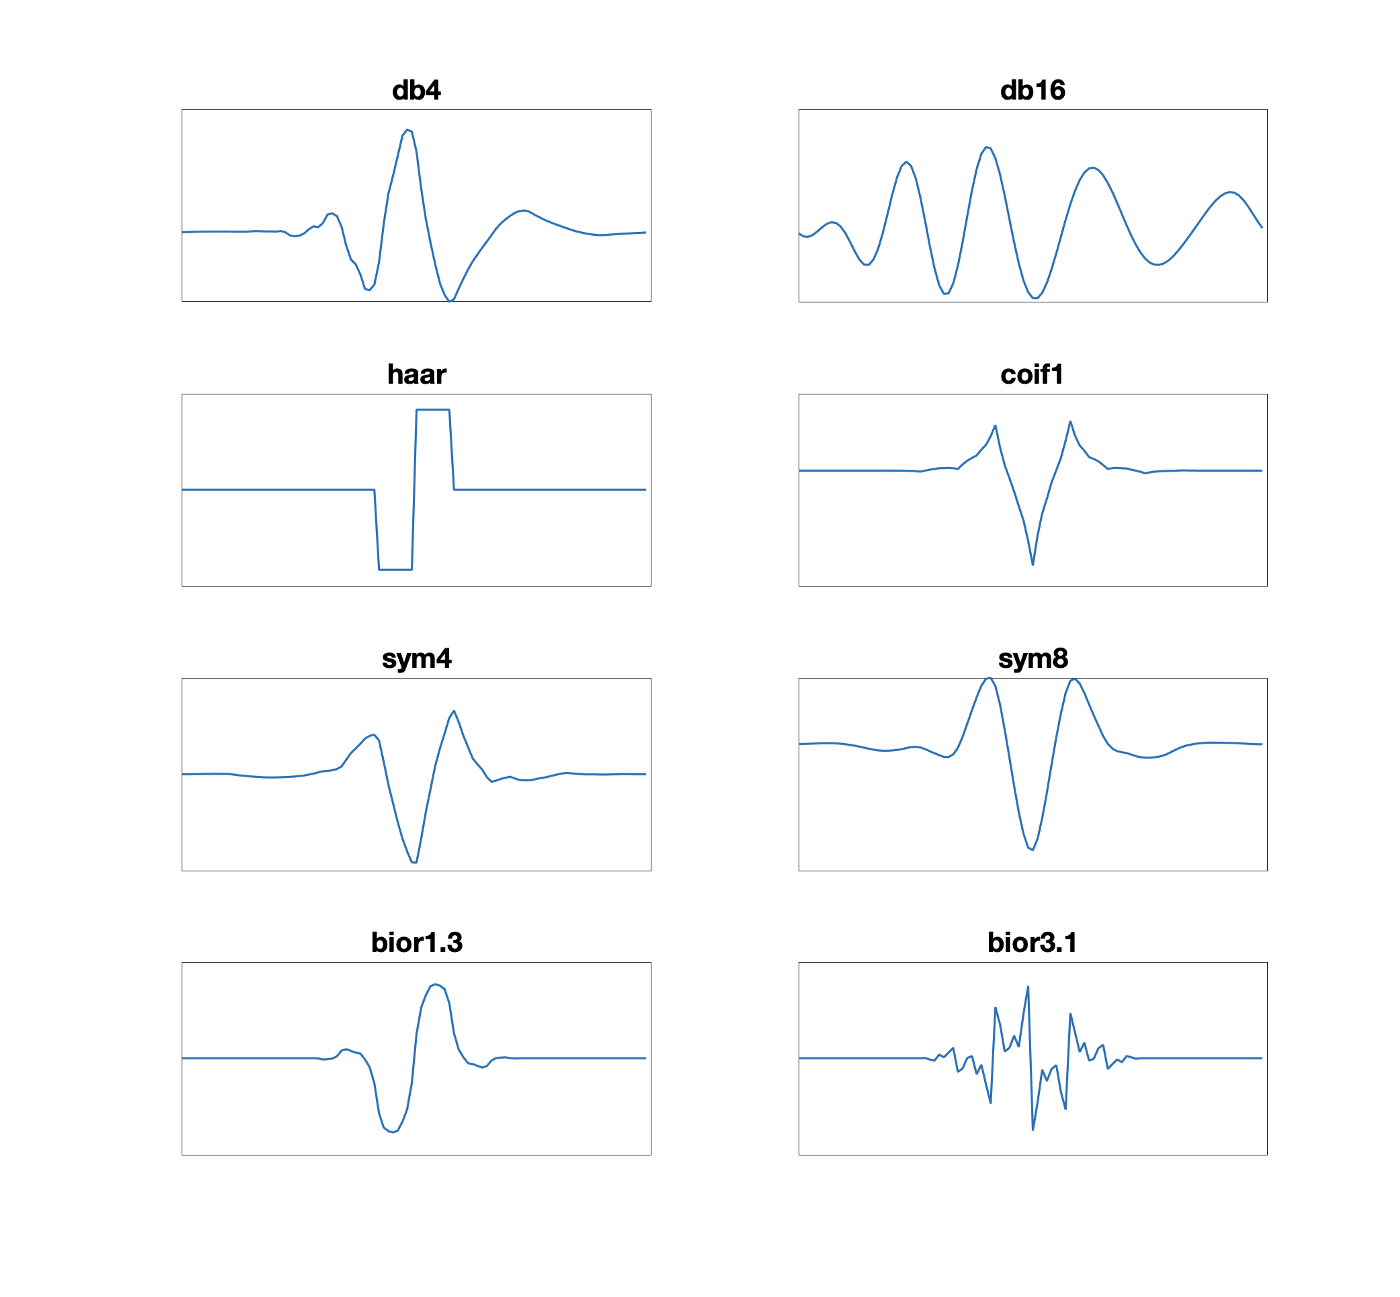
\includegraphics[width=15cm,height=10cm]{Graphics/wavelets.png}
	\caption{Algunos de ejemplos de wavelets.}\label{fig:wavelets}
\end{figure}

Una de las ventajas que tienen las wavelets con respecto a la transformada de Fourier es que 
existe una gran diversidad de wavelets, cada una con sus características, que 
la convierten en la mejor para ciertos escenarios. En la Figura \ref{fig:wavelets} se muestra algunas de las
más conocidas. Sin embargo, dicha variedad constituye también un obstáculo.
Encontrar la wavelet que mejor se adapta al problema en cuestión puede ser un proceso bastante complejo.

\subsection{Familias de wavelets}\label{wavelets-families}

Desde la aparición de la base Haar a principios del siglo pasado, y la explosión de las wavelet en los 
años 1980s, numerosos tipos de wavelet han aparecido en la literatura y softwares especializados en el 
procesamiento de señales. 

Generalmente, los criterios usados para caracterizar a las wavelet son \cite{misiti2007wavelets}:
\begin{enumerate}
	\item El soporte de las funciones $\psi$ y $\phi$ , o su velocidad de convergencia a  cero cuando tienden a 
		infinito.
	\item La simetría, que es útil para evitar desfasajes.
	\item El número de momentos nulos (\textit{vanishing moments}), propiedad de gran importacia en la compresión.
	\item La existencia de la función escala $\phi$.
	\item La ortogonalidad y biortogonalidad.
\end{enumerate}

Muchas aplicaciones de las wavelets explotan su habilidad para aproximar de forma eficiente ciertos tipos de 
funciones. Tal es el caso de la compresión de datos y la reducción y/o eliminación de ruido.
Los momentos nulos o \textit{vanishing moments} son las propiedades de las wavelets que 
hacen posible la representación de funciones suaves con un pequeño número de coeficientes.

Se dice que una wavelet $\psi$ tiene $p$ momentos nulos si:
\begin{equation}
	\int_{-\infty}^{\infty} t^k\psi(t)dt= 0 , \forall 0 \leq k < p.
\end{equation}
Esto significa que la wavelet $\psi$ es ortogonal a cualquier polinomio de grado $p-1$.
Se cumple que si $f$ es regular y $\psi$ tiene suficientes momentos nulos, entonces los coeficientes 
son pequeños, lo cual se puede aprovechar para compresión de datos.

La construcción de wavelets ortogonales con soporte compacto permite el uso del algoritmo de Mallat.
Las  wavelets de Daubechies \cite{daubechies1992}, denotadas por $dbN$ ($N$ indica el orden de la wavelet),
son una de las más conocidas de este tipo. La $db1$, o wavelet Daubechies de primer orden es la wavelet Haar.
Excepto para esta wavelet, las demás de la familia ($dbN$, con $N>1$) no tienen una expresión explícita de la 
función. Además de la ortogonalidad, esta familia tiene las siguientes características:

\begin{enumerate}
	\item El tamaño del soporte de $\phi$ y $\psi$ es $2N-1$, donde $N$ es el número de momentos nulos de $\psi$.
	\item Las $dbN$, exceptuando la wavelet de Haar ($db1$), son asimétricas.
	\item La regularidad aumenta con el orden.
\end{enumerate}

Otra familia de wavelets bastante conocida son las Symlets ($symN$). Estas wavelets son una modificación en la forma
de construir las $dbN$, con el objetivo de lograr simetría.

Las Coiflets ($coifN$) \cite{daubechies1992} son otra familia con propiedades bastante interesantes. Al igual que las dos familias de 
wavelets mencionadas anteriormente, la wavelet $\psi$ de $coifN$ posee $2N$ momentos nulos, pero la función escala
$\phi$ tiene $2N-1$ momentos nulos. Las dos funciones $\phi$ y $\psi$ tienen soporte de longitud $6N-1$.

Las wavelets biortogonales extienden la familia de las ortogonales. De la teoría de filtros se sabe que
la simetría y la reconstrucción perfecta no son compatibles (exceptuando a la wavelet Haar)
cuando se usan el mismo par de filtros, para los procesos 
de descomposición y de reconstrucción de una señal \cite{misiti2007wavelets}. Para poder contrarrestar esta dificultad se usan un par de
wavelets. Una para cada proceso. De este modo es posible buscar las propiedades más deseadas para cada uno de
los procesos por separado en cada wavelet.

Una de las técnicas más conocidas para la construcción de bases wavelet es el método \textit{lifting}, presentado
por primera vez en \cite{lifting}. En este trabajo se propone una nueva generación de wavelets, más general, 
que no son necesariamente traslaciones 
o dilataciones, pero que siguen gozando de todas las beneficiosas propiedades de las wavelets 
de primera generación.
A estas nuevas wavelets se les llama de segunda generación. 

En el esquema \textit{lifting},
un filtro finito, llamado \textit{lifting step}, es usado para 
generar un nuevo par de filtros a partir de otro par existente. Múltiples \textit{lifting steps} pueden ser aplicados
consecutivamente. Dos propiedades interesantes de este esquema son la preservación de la biortogonalidad
y que cualquier wavelet con filtros finitos puede se expresada como una secuencia de \textit{lifting steps}.

\subsection{Wavelets adaptadas a los datos}\label{adapted-wavelets}

En la gran mayoría de las aplicaciones, la selección de las wavelets es fundamental. Se han hecho varios trabajos
para encontrar metodologías y criterios para seleccionar las mejores wavelets en ciertas aplicaciones \cite{ngui2013} \cite{doi:10.1177/14759217211010261}.
Sin embargo, en ocasiones, las wavelets predefinidas que se tienen a mano, no son la mejor opción.
La construcción de una wavelet que posea las propiedades que serían idóneas para un problema puede ser una
vía de solución. Esta es una línea que se ha trabajado en el área de las wavelets, proponiéndose varias
técnicas para la obtención de nuevas funciones basadas en los datos.

El esquema \textit{lifting} ha sido usado en conjunción con otros algoritmos para obtener wavelets 
optimizadas para un conjunto de datos.
En \cite{Grasemann2004} se propone un método basado en un algoritmo genético evolutivo. Este algoritmo codifica las wavelets
como una secuencia de \textit{lifting steps}, para luego ir seleccionando y generando los mejores 
candidatos.

En el caso multidimensional también se han hecho estudios para la obtención de wavelets optimizadas para el problema.
En \cite{Gouze2004} se propone un método para el diseño de filtros \textit{lifting} multidimensionales adaptados a las señales, y  
su aplicación en la compresión de imágenes.

En trabajos más recientes, se han incorporado técnicas de aprendizaje automático para la construcción de filtros.
En \cite{Recoskie2018} se propone un método usando redes neuronales artificiales para aprender funciones 
wavelets directamente de los datos. Esta técnica se aplica al caso unidimensional y se extiende también a otras 
dimensiones.

El Análisis de Componentes Principales (PCA, por sus siglas en inglés) es usado en \cite{floryan}, para la construcción de una base wavelet llamada por los autores como \textit{data-driven wavelet decomposition}
(DDWD). En este método, se impone muy poca estructura a la base que se crea, y cualquier estructura adquirida durante su construcción
es proveniente del conjunto de datos.

La detección de patrones usando wavelets construidas a partir de un patrón es otro de los enfoques trabajados en las wavelets adaptadas a datos.  
En \cite{Mesa2005AdaptedWF} se propone una variante del método de \textit{lifting} para la detección de patrones en señales unidimensionales.
Partiendo de un patrón, se diseñan a través del esquema de \textit{lifting} unas wavelets, y proponen un procedimiento
de detección dividido en tres etapas. Un algoritmo de optimización basado en mínimos cuadrados es usado en \cite{rpeak}
para diseñar una wavelet, que es luego usada en la TWC para detectar un patrón específico. 
Técnicas como las  anteriores pueden ser aplicadas en diversos campos. Por ejemplo, en \cite{Layouni2017} 
se usan wavelets adaptadas a 
patrones para la detección de defectos en tuberías de gas y petróleo.

La DST \cite{Guido2008} es otra de las técnicas que se basa en la construcción de una wavelet (en este caso se le llama \textit{shapelet})
a partir de un patrón. La DST añade al análisis temporal y de frecuencias, el de forma. El concepto de \textit{shapelet}
está inspirado en el de \textit{Spikelet} y \textit{Speechlet}, pero a diferencia de estos si se logra  la condición
de reconstrucción perfecta. Basado en el concepto de \textit{shapelet} el trabajo \cite{lifting-shapelet}, pero usando
el esquema \textit{lifting} para la construcción de los filtros. 

En \cite{Guido2018} se hacen modificaciones a la DST para crear una segunda versión: DST-II. Esta última
comparte muchas de las características de la primera versión, excepto por las condiciones 
de detección (\textit{matching}).
Esta nueva variante añade las condiciones antes mencionadas de forma tal que el producto escalar inherente al algoritmo
de Mallat durante el cálculo de la transformada sea $0$.

Recientemente, en \cite{Guido2021}, el mismo autor propone una mejora a las dos versiones anteriores de la 
DST e introduce la tercera generación: DST-III. Esta variante, a diferencia de las dos anteriores, permite 
la creación de \textit{shapelets} casi simétricas. 



\chapter{Propuesta}\label{chapter:proposal}

El principal objetivo de este trabajo es la construcción de wavelets adaptadas a patrones usando el algoritmo de
la DST-II \cite{Guido2018} para su posterior detección en señales. En este capítulo se presenta una explicación 
detallada del algoritmo, así como varias propuestas para su extensión para el uso en señales bidimensionales para
ser luego aplicada específicamente para la detección de masas en mamografías.

\section{Aspectos generales de las DSTs}

La DST-II es una modificación de la DST. Por este motivo ambas comparten muchos puntos y de forma similar 
a la DWT poseen los siguientes componentes y características \cite{Guido2008}\cite{Guido2018}:

\begin{itemize}
	\item El par de filtros $p[\cdot]$ y $q[\cdot]$ donde $q_k = (-1)^k p_{N-k-1}$. 
		Estos representan ,respectivamente, los filtros \textit{low-pass} y \textit{high-pass} y  
		usados en conjunto con el algoritmo de Mallat \cite{} para obtener la transformada de la 
		señal, exactamente igual a como se hace en la DWT, donde se les conoce usualmente como $h[\cdot]$ y
		$g[\cdot]$.
	\item El par de filtros $\bar p[\cdot]$  y $\bar q[\cdot]$ que son los filtros usados para la etapa 
		de síntesis de la señal. En el ámbito de la DWT, se conocen como $\bar h[\cdot]$ y $\bar g[\cdot]$.
	\item Las funciones $\Gamma(x)=\sum_k p_k \Gamma(2N-k)$ y $\Theta(x)=\sum_k q_k \Theta(2N-k)$ conocidas 
		como \textit{major shapelet} y \textit{minor shapelet} respectivamente. Las mismas conrresponden a las
		funciones de \textit{scaling} $\phi(x)$ y \textit{wavelet} $\psi(x)$ en la DWT.
	\item Las condiciones $\bar P[z] = Q[-z]$, $\bar Q[z]=-P[-z]$ y $\bar P[z]P[z] + \bar Q[z]Q[z]=2z^{-N+1}$,
		todas en el dominio de $Z$, implican que $p[\cdot]$, $q[\cdot]$, $\bar p[\cdot]$  y $\bar q[\cdot]$
		forman un banco de filtro de construcción perfecta (PRFB por sus siglas en inglés).
\end{itemize}

Otro aspecto importante de las DST es que el resultado de la misma al procesar una señal $s[\cdot]$ produce dos 
señales de igual longitud igual a la mitad de la señal de entrada $s[\cdot]$. La primera mitad corresponde a 
\textit{master} y la segunda a \textit{second-rated}. La concatenación de las mismas caracteriza a las DST
y corresponden a los coeficientes de aproximación y detalles en la DWT respectivamente.

El procedimiento para obtener el filtro $q[\cdot]$ de la DST-II es similar al usado para generar el mismo filtro
en la DST. Sin embargo, la condición basada en el \textit{matching} fractal es sustuida por un par de condiciones
conocidas como \textit{matching conditions}.


\section{Formulación de la DST-II}\label{algoritmo:dst-2}

Como se menciona en la sección anterior, el procedimiento para obtener el filtro $q[\cdot]$ en la DST y DST-II
es distinto. Para el cálculo del mismo se establecen las siguientes restricciones:

\begin{itemize}
	\item El tamaño del filtro debe ser ser $N \geq 6$. Esta restricción es necesaria por el hecho de que la 
		DST-II tiene $\frac{N}{2}-2$  momentos nulos su \textit{minor shapelet}, equivalente a función \textit{wavelet}
		en la DWT. Por tanto, si $N<6$, no se tendrían momentos nulos en esa función, distorsionando la transformada.
	\item El tamaño del filtro deber ser par, al igual que en la DWT. De lo contrario, no se puede obtener una 
		reconstrucción perfecta.
	\item El patrón que se quiere detectar $m[\cdot]$, debe tener tamaño impar igual a $N+1$.
\end{itemize}

Teniendo en cuenta las restricciones anteriores, el procedimiento para la obtención del filtro $q[\cdot]$ en la DST-II 
es el siguiente:

\begin{itemize}
	\item \textbf{Paso 1:} Forzar que el filtro posea energía unitaria
		\begin{equation}\label{eq:unitary-energy}
			\sum_{k=0}^{N-1}q_k^2 = 1.
		\end{equation}
	\item \textbf{Paso 2:} Imponer $\frac{N}{2} -2 $ momentos nulos para la \textit{mejor shapelet}
		\begin{equation}\label{eq:vanishing-moments}
			\sum_{k=0}^{N-1}q_{k}k^b = 0
		\end{equation}
		donde $b=0,1,\dotsc,\frac{N}{2}-3$.
	\item \textbf{Paso 3:} Definir las condiciones de otogonalidad
		\begin{equation}\label{eq:orthogonality}
			\sum_{k=0}^{N-1} q_{k}q_{k+2l} = \delta_{0,1}
		\end{equation}
		donde $\delta$ es el delta de Dirac y $l\in Z$.
	\item \textbf{Paso 4:} Agregar las condiciones de \textit{matching}
		\begin{equation}\label{eq:original-matching-1}
			\sum_{k=0}^{N-1} q_{k}m_{k} = 0
		\end{equation}
		\begin{equation}\label{eq:original-matching-2}
			\sum_{k=0}^{N-1} q_{k}m_{k+1} = 0
		\end{equation}
	\item \textbf{Paso 5:} Agrupar todas las ecuaciones definidas anteriormente y resolver el sistema de ecuaciones
		no lineales $N$ ecuaciones y $N$ incógnitas para obtener el filtro $q[\cdot]$.
	\item \textbf{Paso 6:} Obtener $p[\cdot]$ como $p_k=(-1)^{k+1}q_{N-k-1}$ y 
		después a partir de $q[\cdot]$ y $p[\cdot]$ calcular los filtros $\bar q[\cdot]$ y $\bar p[\cdot]$.
	\item \textbf{Paso 7:} Como paso opcional, si se desea conocer la forma de la \textit{major} y \textit{minor}
		\textit{shapelet} se pueden calcular $\Gamma(x)=\sum_k p_k \Gamma(2N-k)$ y $\Theta(x)=\sum_k q_k \Theta(2N-k)$.
\end{itemize}

En esencia la DST-II corresponde a la transformada de Daubechies, cambiando de de los momentos nulos por las
condiciones de \textit{matching},\ref{eq:original-matching-1} y \ref{eq:original-matching-2}. Estas están definidas de forma tal que el
producto inherente como resultado del cómputo de la DST-II, basado en el algoritmo de Mallat, reaccione ante 
la presencia del patrón $m[\cdot]$.

El algoritmo de la DST-II y su inversa es exactamente el mismo que para la DWT, por lo que la complejidad computacional
es la misma.

\section{Solución numérica del sistema de ecuaciones no lineales}\label{numerical-solution}

Solucionar un sistema de ecuaciones no lineales, es una situación que se evita siempre que sea posible. Por lo general
se trata de simplificar el sistema sustituyendolo con uno lineal \cite{Burden2016}. Sin embargo, esto no siempre es posible y se debe abordar el problema de
forma directa. En el caso de la construcción del filtro $q$, no es posible simplificar el sistema, pues violaría
las condiciones de su propia definición. Por este motivo es necesario seleccionar métodos numéricos para la
solución del sistema definido en \ref{algoritmo:dst-2}.

El método de Newton es de los más simples y conocidos para resolver ecuaciones y se puede extender al caso de varias
variables. Su convergencia suele ser rápida una vez que se obtiene una aproximación que está cerca de la solución
verdadera. Sin embargo, no siempre es fácil determinar un conjunto de valores iniciales. Además, otra debilidad
significativa para resolver sistemas de ecuaciones no lineales es la necesidad de determinar en cada iteración 
una matriz y resolver un sistema lineal de tamaño $n\times n$ \cite{Burden2016}. 

Existe otra clase de algoritmos llamados métodos de Newton inexactos o cuasi-Newton. Estos métodos reemplazan la
matriz jacobiana en el método de Newton con una matriz de aproximación que se actualiza fácilmente en 
cada iteración. La desventaja de estos métodos es que la convergencia cuadrática del método de Newton se pierde,
al ser reemplazada, en general, mediante una convergencia superlineal. Otra desventaja es que a diferencia 
del método de Newton, los métodos quasi-Newton no se autocorrigen. En muchos casos, el método de Newton
corrige el error de redondeo con iteraciones sucesivas. Sin embargo, en muchos escenarios, la reducción 
de la convergencia es un precio aceptable a pagar para reducir la cantidad de cálculos \cite{Burden2016}. 

Entre los métodos que pertenecen a esta clase de algoritmos se encuentran Broyden1 y Broyden2. El primero es conocido
como el método bueno de Broyden, y usa el primer jacobiano de Broyden para la aproximación. El segundo se conoce
como el método malo de Broyden, en vez del primer jacobiano, usa el segundo \cite{broyden}.

El método de Anderson también llamado Anderson \textit{mixing} \cite{Eyert1996} y el de Krylov también son métodos inexactos de Newton. 
Este último usa la aproximación de Krylov para el inverso del jacobiano y suele ser una buena opción para problemas
con de gran escala \cite{kelley1995iterative}.

Aunque el sistema planteado en \ref{algoritmo:dst-2} tiene exactamente la misma cantidad de ecuaciones que de 
incógnitas, algoritmos como el método híbrido de Powell y el algoritmo de Levenberg-Marquardt pueden 
ser usados para encontrar una solución. Ambos métodos están diseñados para problemas de mínimos cuadrados no lineales.

El algoritmo de Levenberg-Marquardt combina dos algoritmos de minimización numérica:
gradiente descendiente y el método de Gauss-Newton. El método Levenberg-Marquardt actúa más como gradiente 
descendiente cuando los parámetros están lejos del valor óptimo, y a medida que los valores se acercan 
al óptimo, actúa más como el método de Gauss-Newton \cite{madsen2004methods}.

El método híbrido de Powell, de forma similar a Levenberg-Marquardt es una combinación de gradiente descendiente y Gauss-Newton.
Sin embargo, en este la selección es controlada por el uso de una región de confianza \cite{madsen2004methods}.

\section{Medida de similitud para la detección}

Al estar basada en la DWT, el análisis temporal y de frecuencia de la DST-II es exactamente igual que al de la DWT.
Sin embargo, la mayor novedad de este algoritmo, es la capacidad de reaccionar ante la presencia de 
patrones específicos, facilitando su detección. El proceso es bastante sencillo :
mientras más cercano a $0$ esté el coeficiente de la parte \textit{second-rated} de la transformada, más se parece
la sección de la señal analizada $s[\cdot]$ al patrón $m[\cdot]$ que se quiere detectar. En \cite{Guido2018} se
propone la siguiente medida de similitud para la detección de las muestras que cumplan con estas características:

\begin{equation}
	\mathbb{S} = e^{-{(|DST-II(s[\cdot])|)}^{\alpha}} \ 0 < \alpha \leq 1
\end{equation}\label{eq:s-heuristic}

Mientras más cercano sea $\mathbb{S}$ a 0 o 1, respectivamente, menos o más se parece el segmento de
la señal analizada $s[\cdot]$ a $m[\cdot]$.

Según \cite{Guido2018}, para el primer nivel de la DST-II, si $\mathbb{S}_{_k}=1$ para algún $k=0,1,2,\ldots$
con $k$ que pertenece a la segunda parte de la transformada ( \textit{second-rated} ), esto implica que 
que el patrón empieza en la posición $s_{2k-1}$ o $s_{2k}$. Un aspecto importante es que la búsqueda de 
ceros en la DST-II, o unos en $\mathbb{S}$, solo se lleva a cabo en la segunda sub-banda de la transformada,
es decir, en el segmento perteneciente a la \textit{second-rated}.

\section{Ejemplo numérico del diseño de la DST-II}

\begin{figure} 
	\centering
	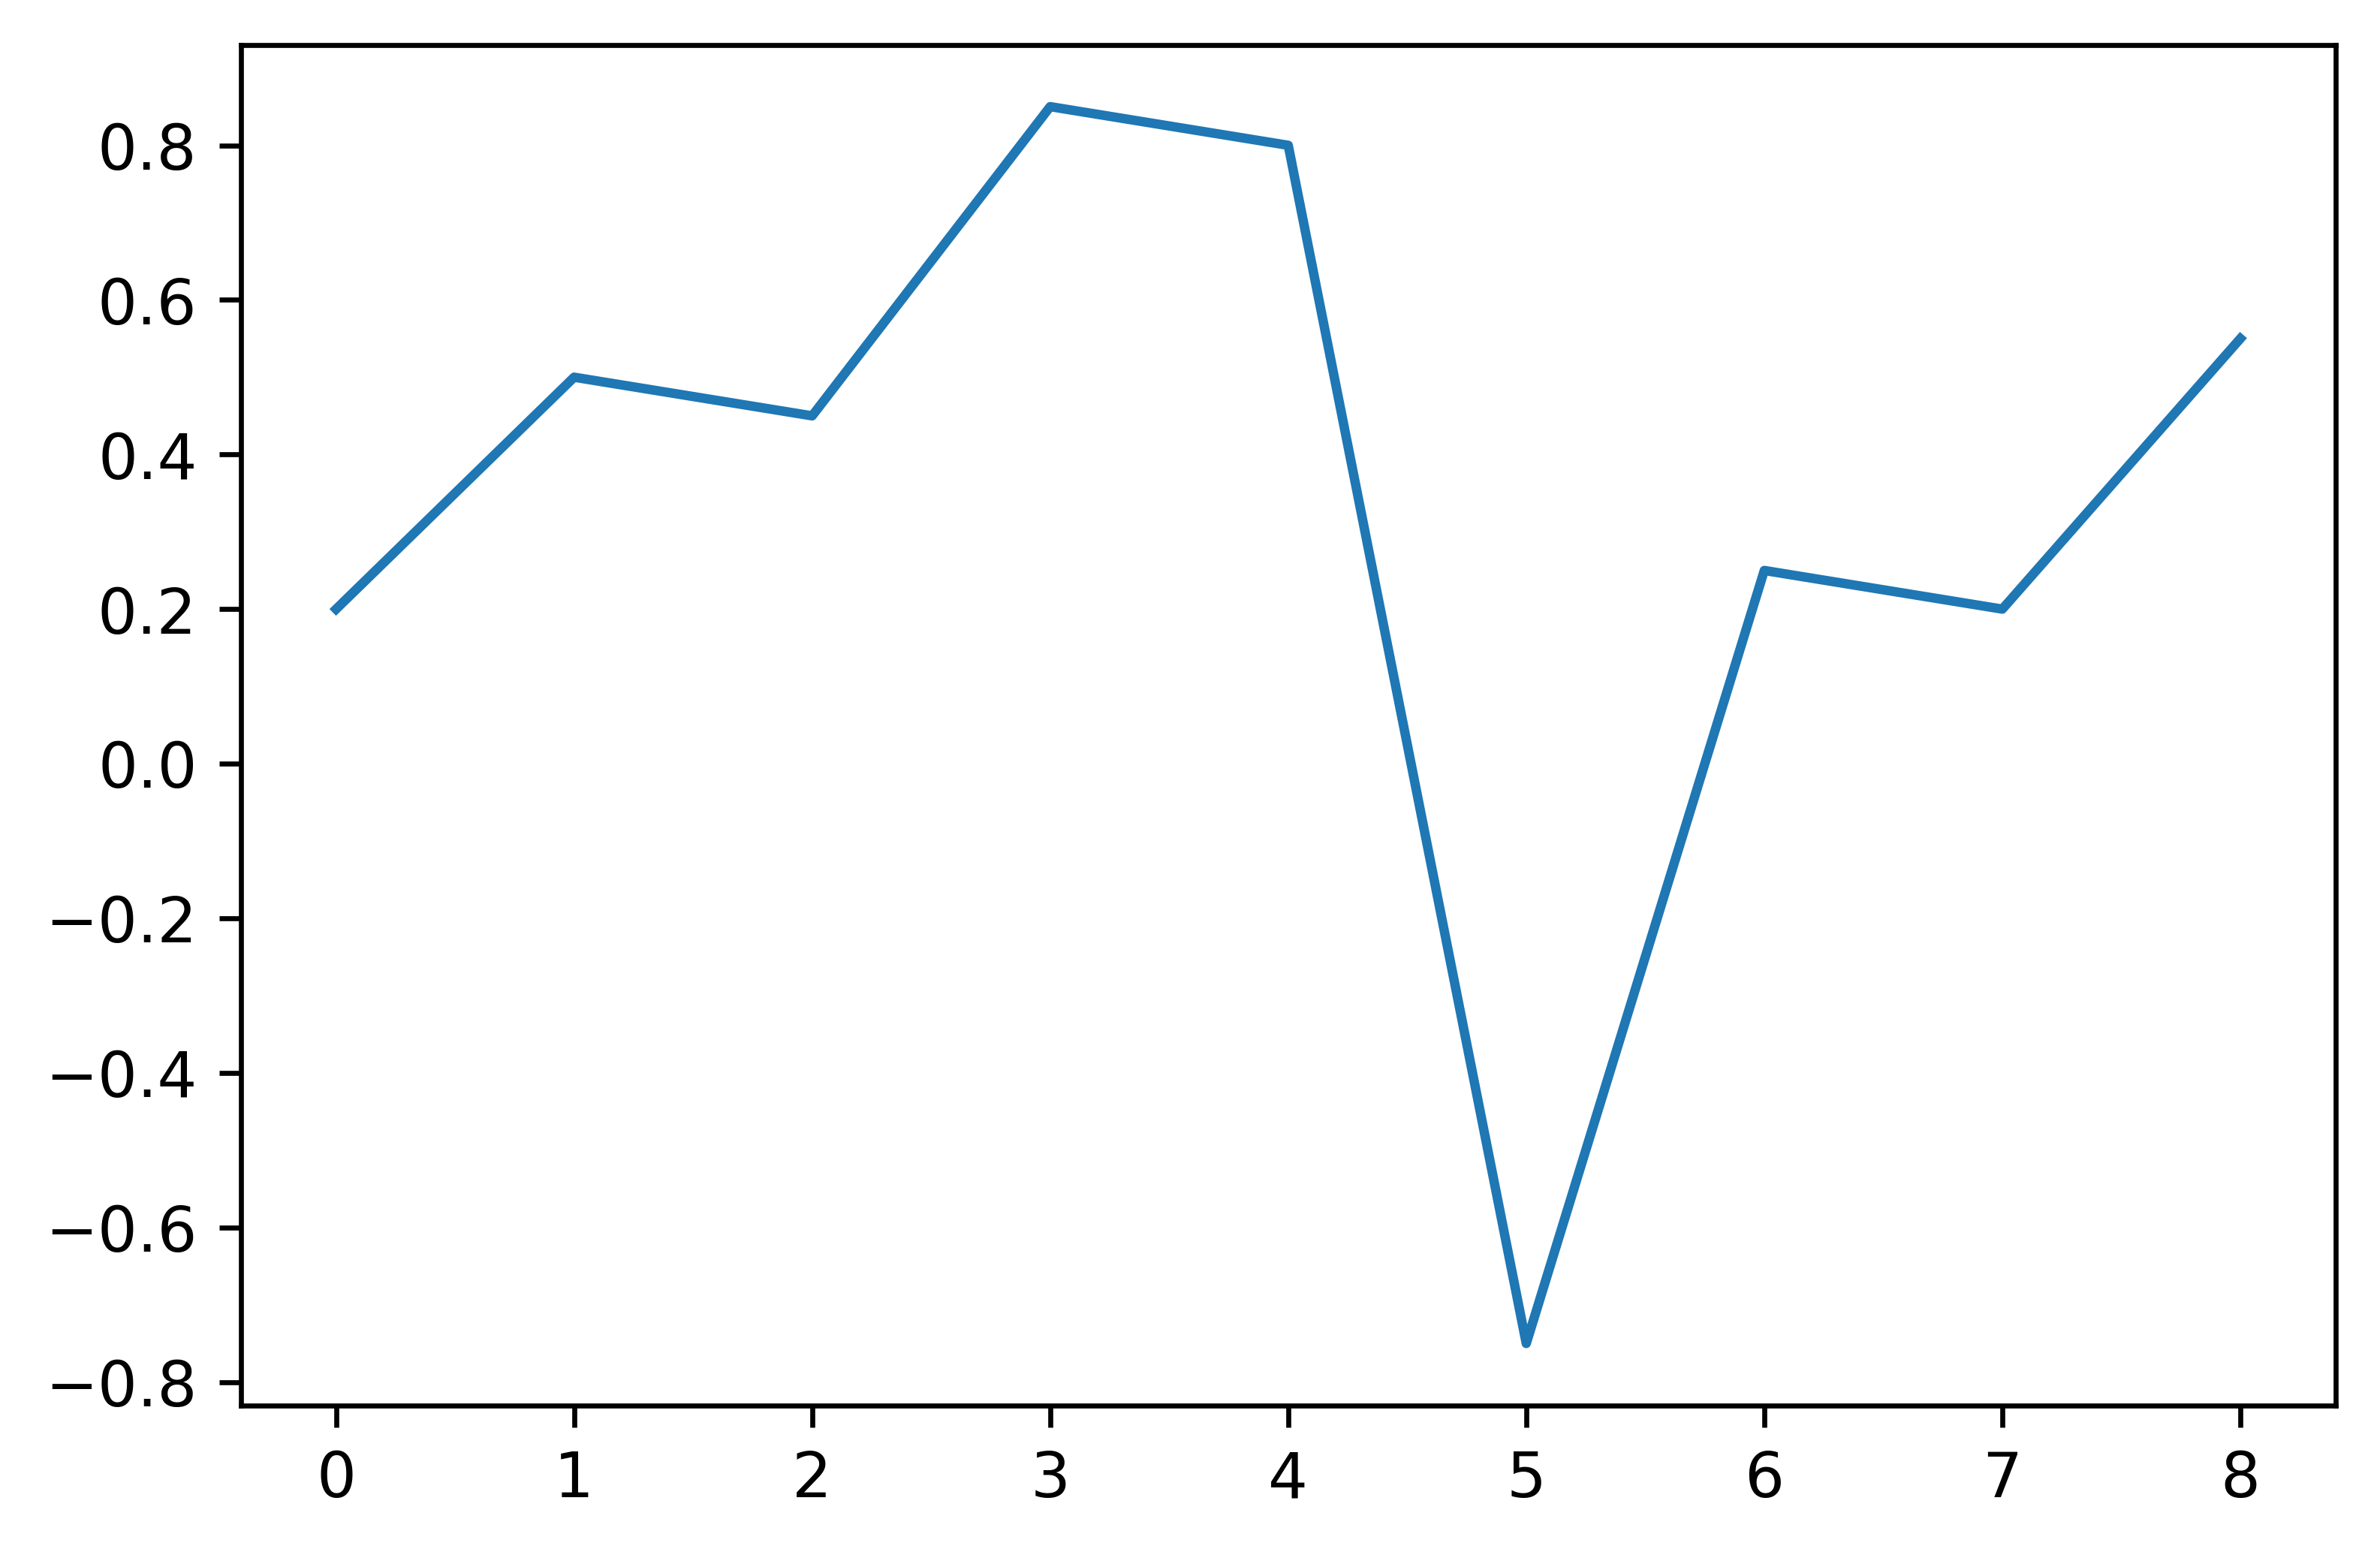
\includegraphics[scale=0.8]{Graphics/guido20118-pattern.png}
	\caption{Patrón usado en \cite{Guido2018} con valores [0.20, 0.50, 0.45, 0.85, 0.80, -0.75, 0.25, 0.20, 0.55]} \label{fig:Guido2018-pattern}
\end{figure}

En esta sección se describe paso a paso la construcción del filtro $q[\cdot]$ para la detección del
patrón $m[\cdot]$ que se muestra en \ref{fig:Guido2018-pattern}. El método numérico usado para hallar
la solución al sistema de eucaciones no lineales es Levenberg-Marquardt.

Según los pasos descritos en \ref{algoritmo:dst-2}, las ecuaciones del sistema son las siguientes:

\begin{itemize}
	\item \textbf{Paso 1:} La ecuación de la energía unitaria \ref{eq:unitary-energy}
		\begin{equation}
			q_0^2 + q_1^2 + q_2^2 + q_3^2 + q_4^2 + q_5^2 + q_6^2 + q_7^2 - 1 = 0
		\end{equation}
	\item \textbf{Paso 2:} Dos ecuaciones de momentos nulos \ref{eq:vanishing-moments}
		\begin{equation}
			q_1 + q_2 + q_3 + q_4 + q_5 + q_6 + q_7  = 0
		\end{equation}
		\begin{equation}
			q_1 + 2q_2 + 3q_3 + 4q_4 + 5q_5 + 6q_6 + 7q_7 = 0
		\end{equation}
	\item \textbf{Paso 3:} Tres ecuaciones para las condiciones de ortogonalidad \ref{eq:orthogonality}
		\begin{equation}
			q_0q_2 + q_1q_3 + q_2q_4 + q_3q_5 + q_4q_6 + q_5q_7 = 0
		\end{equation}
		\begin{equation}
			q_0q_4 + q_1q_5 + q_2q_6 + q_3q_7 = 0
		\end{equation}
		\begin{equation}
			q_0q_6 + q_1q_7 = 0
		\end{equation}
	\item \textbf{Paso 4:} Las condiciones de \textit{matching} 
		\begin{equation}
			0.2q_0 + 0.5q_1 + 0.45q_2 + 0.85q_3 + 0.8q_4 - 0.75q_5 + 0.25q_6 + 0.2q_7
		\end{equation}
		\begin{equation}
			0.5q_0 + 0.45q_1 + 0.85q_2 + 0.8q_3 - 0.75q_4 + 0.25q_5 + 0.2q_6 + 0.55q_7
		\end{equation}
	\item \textbf{Paso 5:} Agrupando todas las ecuaciones se obtiene el sistema de ecuaciones no lineales
		\begin{equation}\label{eq:system}
			\left\{ \begin{array}{rcl}
						q_0^2 + q_1^2 + q_2^2 + q_3^2 + q_4^2 + q_5^2 + q_6^2 + q_7^2 - 1 = 0 \\
						q_1 + q_2 + q_3 + q_4 + q_5 + q_6 + q_7  = 0 \\
						q_1 + 2q_2 + 3q_3 + 4q_4 + 5q_5 + 6q_6 + 7q_7 = 0 \\
						q_0q_2 + q_1q_3 + q_2q_4 + q_3q_5 + q_4q_6 + q_5q_7 = 0 \\
						q_0q_4 + q_1q_5 + q_2q_6 + q_3q_7 = 0 \\
						q_0q_6 + q_1q_7 = 0 \\
						0.2q_0 + 0.5q_1 + 0.45q_2 + 0.85q_3 + 0.8q_4 - 0.75q_5 + 0.25q_6 + 0.2q_7 \\
						0.5q_0 + 0.45q_1 + 0.85q_2 + 0.8q_3 - 0.75q_4 + 0.25q_5 + 0.2q_6 + 0.55q_7 \\
					\end{array}
				\right.
			\end{equation}
\end{itemize}

Luego de resolver el \ref{eq:system} se obtiene como solución el siguiente vector para $q[\cdot]$:

$$
	\begin{array}{lcl}
		q[\cdot] = \{ 0.6847497581435479, 0.22696568380592325, 0.14564494606257186,  \\ 
					-0.6216329207785873, 0.18823424339300499, -0.0553137649474309, \\ 
					-0.05756235031820252, 0.1736641627827206 \}
	\end{array}
$$

Una vez que se tiene el valor de $q[\cdot]$ se procede a calcular el resto de los filtros:

$$
	\begin{array}{lcl}
		p[\cdot] = \{  -0.17366416278272068, -0.05756235031820252, 0.0553137649474309, \\ 
					0.18823424339300499, 0.6216329207785873, 0.14564494606257186, \\
					-0.22696568380592325, 0.684749758143547\}
	\end{array}
$$

$$
	\begin{array}{lcl}
		\bar p[\cdot] = \{ -0.17366416278272068, 0.6847497581435479, -0.22696568380592325, \\ 
							0.14564494606257186, 0.6216329207785873, 0.18823424339300499, \\ 
							0.0553137649474309, -0.05756235031820252 \}
	\end{array}
$$

$$
	\begin{array}{lcl}
		\bar q[\cdot] = \{ -0.6847497581435479, 0.22696568380592325, -0.14564494606257186,\\
			-0.6216329207785873, -0.18823424339300499, -0.0553137649474309, \\ 
		0.05756235031820252, 0.17366416278272068 \}
	\end{array}
$$

Un vez se obtienen los filtros, es posible realizar la DST-II sobre cualquier señal para detectar la presencia
del patrón $m[\cdot]$. Como paso opcional si se quiere obtener las funciones \textit{major} y \textit{minor}
se procedería a resolver los sistemas formados por las eucaciones  $\Gamma(x)=\sum_k p_k \Gamma(2N-k)$ y 
$\Theta(x)=\sum_k q_k \Theta(2N-k)$.

Para demostrar el uso de las DST-II en la detección de patrones y formas, el patrón $m[\cdot]$ \ref{fig:Guido2018-pattern} fue
insertado en la señal $s[\cdot]$, dando como resultado la siguiente señal \ref{fig:example-guido-signal}:

\begin{equation}
	s[x] = \left\{ \begin{array}{rcl}
			\cos{\frac{27\pi x}{8}}\sin{\frac{75\pi x}{8}} & \mbox{si} &  0\leq x \leq 40 \\
			m[x]    &    \mbox{si}     &     41\leq x \leq 49     \\
			\cos{\frac{295\pi x}{32}}\sin{\frac{105\pi x}{32}} & \mbox{si} &  50\leq x \leq 63 \\
					 \end{array}
	\right.
\end{equation}

\begin{figure}
	\centering
	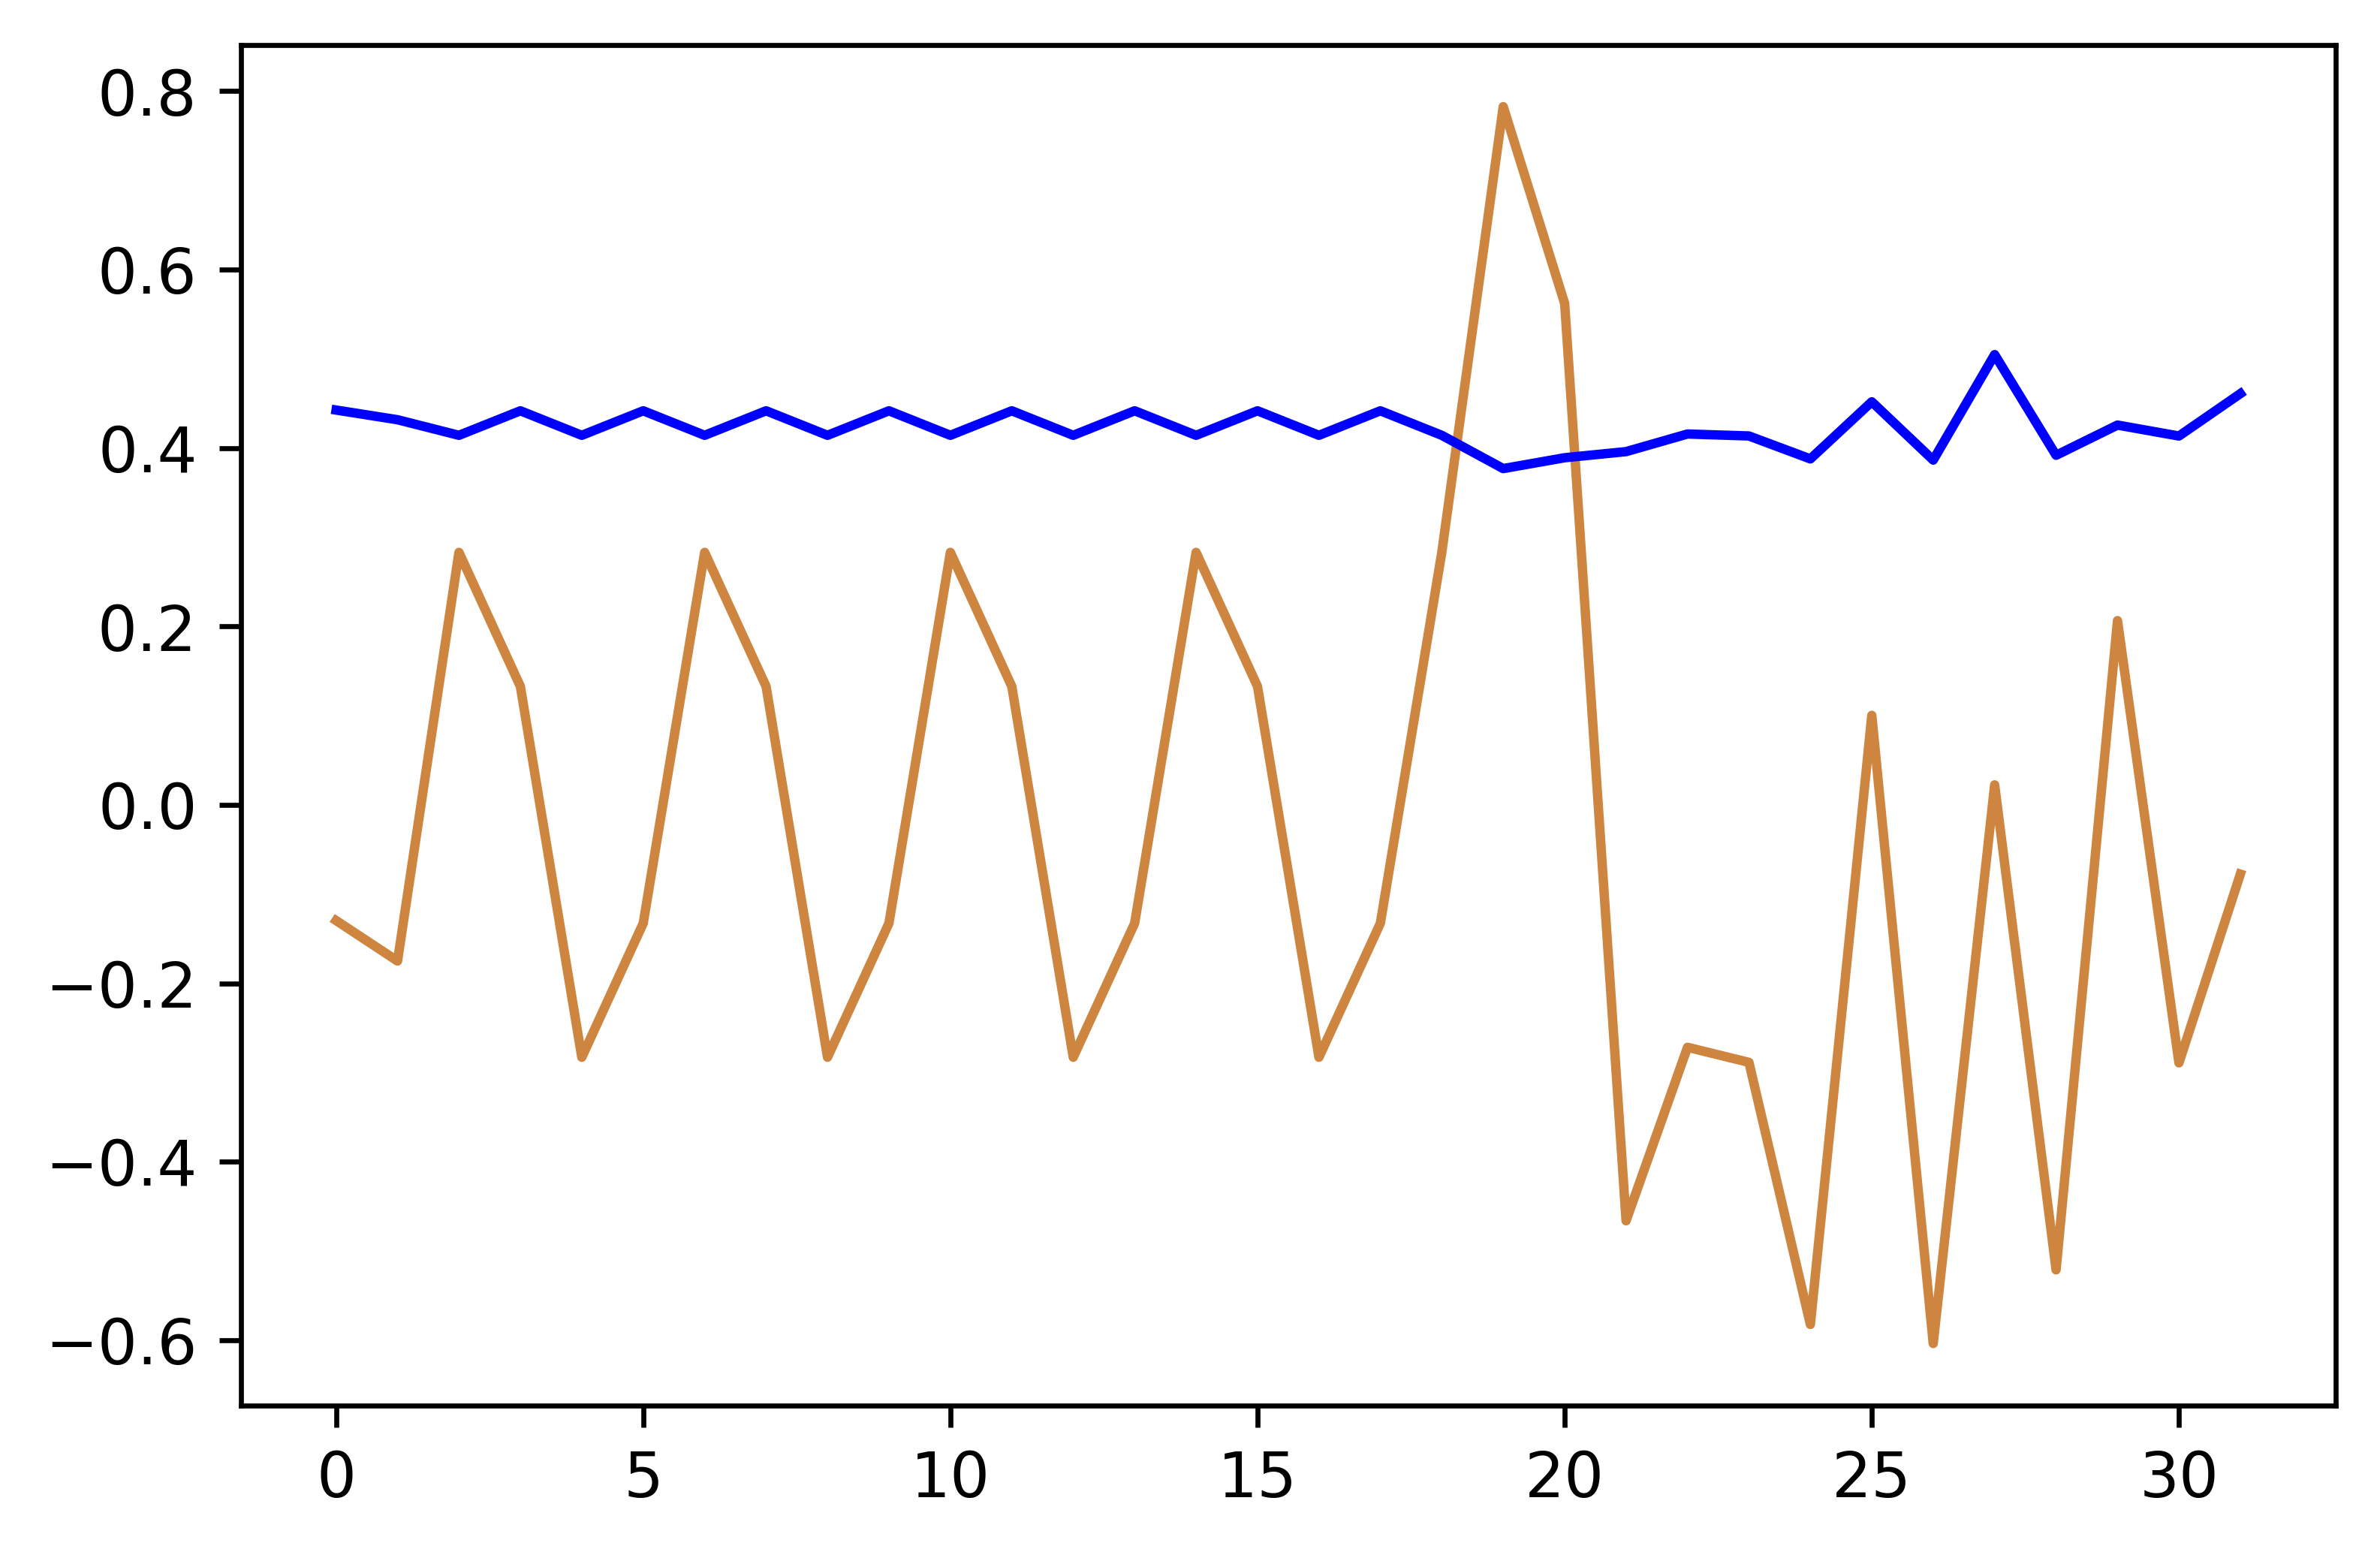
\includegraphics[scale=0.8]{Graphics/example-guido-signal-dst-s-wrong-matching.png}
	\caption{DST-II y medida $\mathbb{S}$ usando los las ecuaciones de \textit{matching} \ref{eq:original-matching-1} \ref{eq:original-matching-2}} \label{fig:example-guido-signal-dst-s-wrong-matching}
\end{figure}


La figura \ref{fig:example-guido-signal-dst-s-wrong-matching} muestra el resultado de la DST-II sobre la señal $s[\cdot]$.
El gráfico color marrón es la sección \textit{second-rated} del resultado de ls DST-II sobre $s[\cdot]$.
El de color azul conrresponde a la medida $\mathbb{S}$ sobre los coeficiente de la \textit{second-rated}. 
Sin embargo, en este gráfico se puede observar que en $\mathbb{S}$ no existe un pico que sobresale del resto del
gráfico, a diferencia de como sucede en el ejmplo de \cite{Guido2018}. De hecho, el punto más alto
se alcanza en el coeficiente número 27, que no corresponde con la ubicación del patrón en la señal 
original. Además, en esta posición $\mathbb{S}=0.5046662398523433$, lo cual implica que no se detecta el patrón.

\subsection{Reajuste en las condiciones de \textit{matching}}

La DST-II está diseñada para que las condiciones de \textit{matching} \ref{eq:matching-1} \ref{eq:matching-2} 
permitan obtener un valor lo más cercano a $0$ cuando se realiza la convolución entre el filtro $q[\cdot]$
y el patrón $m[\cdot]$. Sin embargo, es necesario hacer un pequeño cambio a las ecuaciones \ref{eq:matching-1}
para que esto funcione \ref{eq:matching-1}.

De \ref{eq:mallat-details} se tiene que la convolución se hace multiplicando el filtro de atrás hacia adelante 
con la sección de la señal que se está procesando. Por lo que en vez usar las ecuaciones \ref{eq:matching-1}
y \ref{eq:matching-2} se usan las siguientes:

\begin{equation}\label{eq:matching-1}
	\sum_{k=1}^{N} q_{N-k}m_{k} = 0
\end{equation}
\begin{equation}\label{eq:matching-2}
	\sum_{k=1}^{N} q_{N-k}m_{k-1} = 0
\end{equation}

Usando estas nuevas fórmulas, se obtienen las siguientes ecuaciones para el ejemplo del patrón \ref{fig:Guido2018-pattern}:

\begin{equation}
	0.2q_0 + 0.25q_1 - 0.75q_2 + 0.8q_3 + 0.85q_4 + 0.45q_5 + 0.5q_6 + 0.2q_7
\end{equation}
\begin{equation}
	0.55q_0 + 0.2q_1 + 0.25q_2 - 0.75q_3 + 0.8q_4 + 0.85q_5 + 0.45q_6 + 0.5q_7
\end{equation}

Después de sustuir las ecuaciones de \textit{matching} anteriores en \ref{eq:system} se resuelve el sistema
de ecuaciones no lineales y se obtiene la siguiente solución:

$$
	\begin{array}{lcl}
		q[\cdot] = \{ 0.8505813325748994, -0.24960592535063272, 0.22199103863909603,\\ 
			0.29414386817594423, -0.10204570231699035, -0.25121801175290576, \\ 
		0.019678016661321896, 0.06705671594416668 \}
	\end{array}
$$

Luego, a partir de $q$ se obtienen:

$$
	\begin{array}{lcl}
		p[\cdot] = \{ -0.06705671594416668, 0.019678016661321896, 0.25121801175290576,\\ 
			-0.10204570231699035, -0.29414386817594423, 0.22199103863909603, \\ 
			0.24960592535063272, 0.8505813325748994\}
	\end{array}
$$

$$
	\begin{array}{lcl}
		\bar p[\cdot] = \{ -0.06705671594416668, 0.8505813325748994, 0.24960592535063272,\\ 
			0.22199103863909603, -0.29414386817594423, -0.10204570231699035,\\ 
		0.25121801175290576, 0.019678016661321896 \}
	\end{array}
$$

$$
	\begin{array}{lcl}
		\bar q[\cdot] = \{ -0.8505813325748994, -0.24960592535063272, -0.22199103863909603,\\
			0.29414386817594423, 0.10204570231699035, -0.25121801175290576, \\ 
		-0.019678016661321896, 0.06705671594416668 \}
	\end{array}
$$

\begin{figure} 
	\centering
	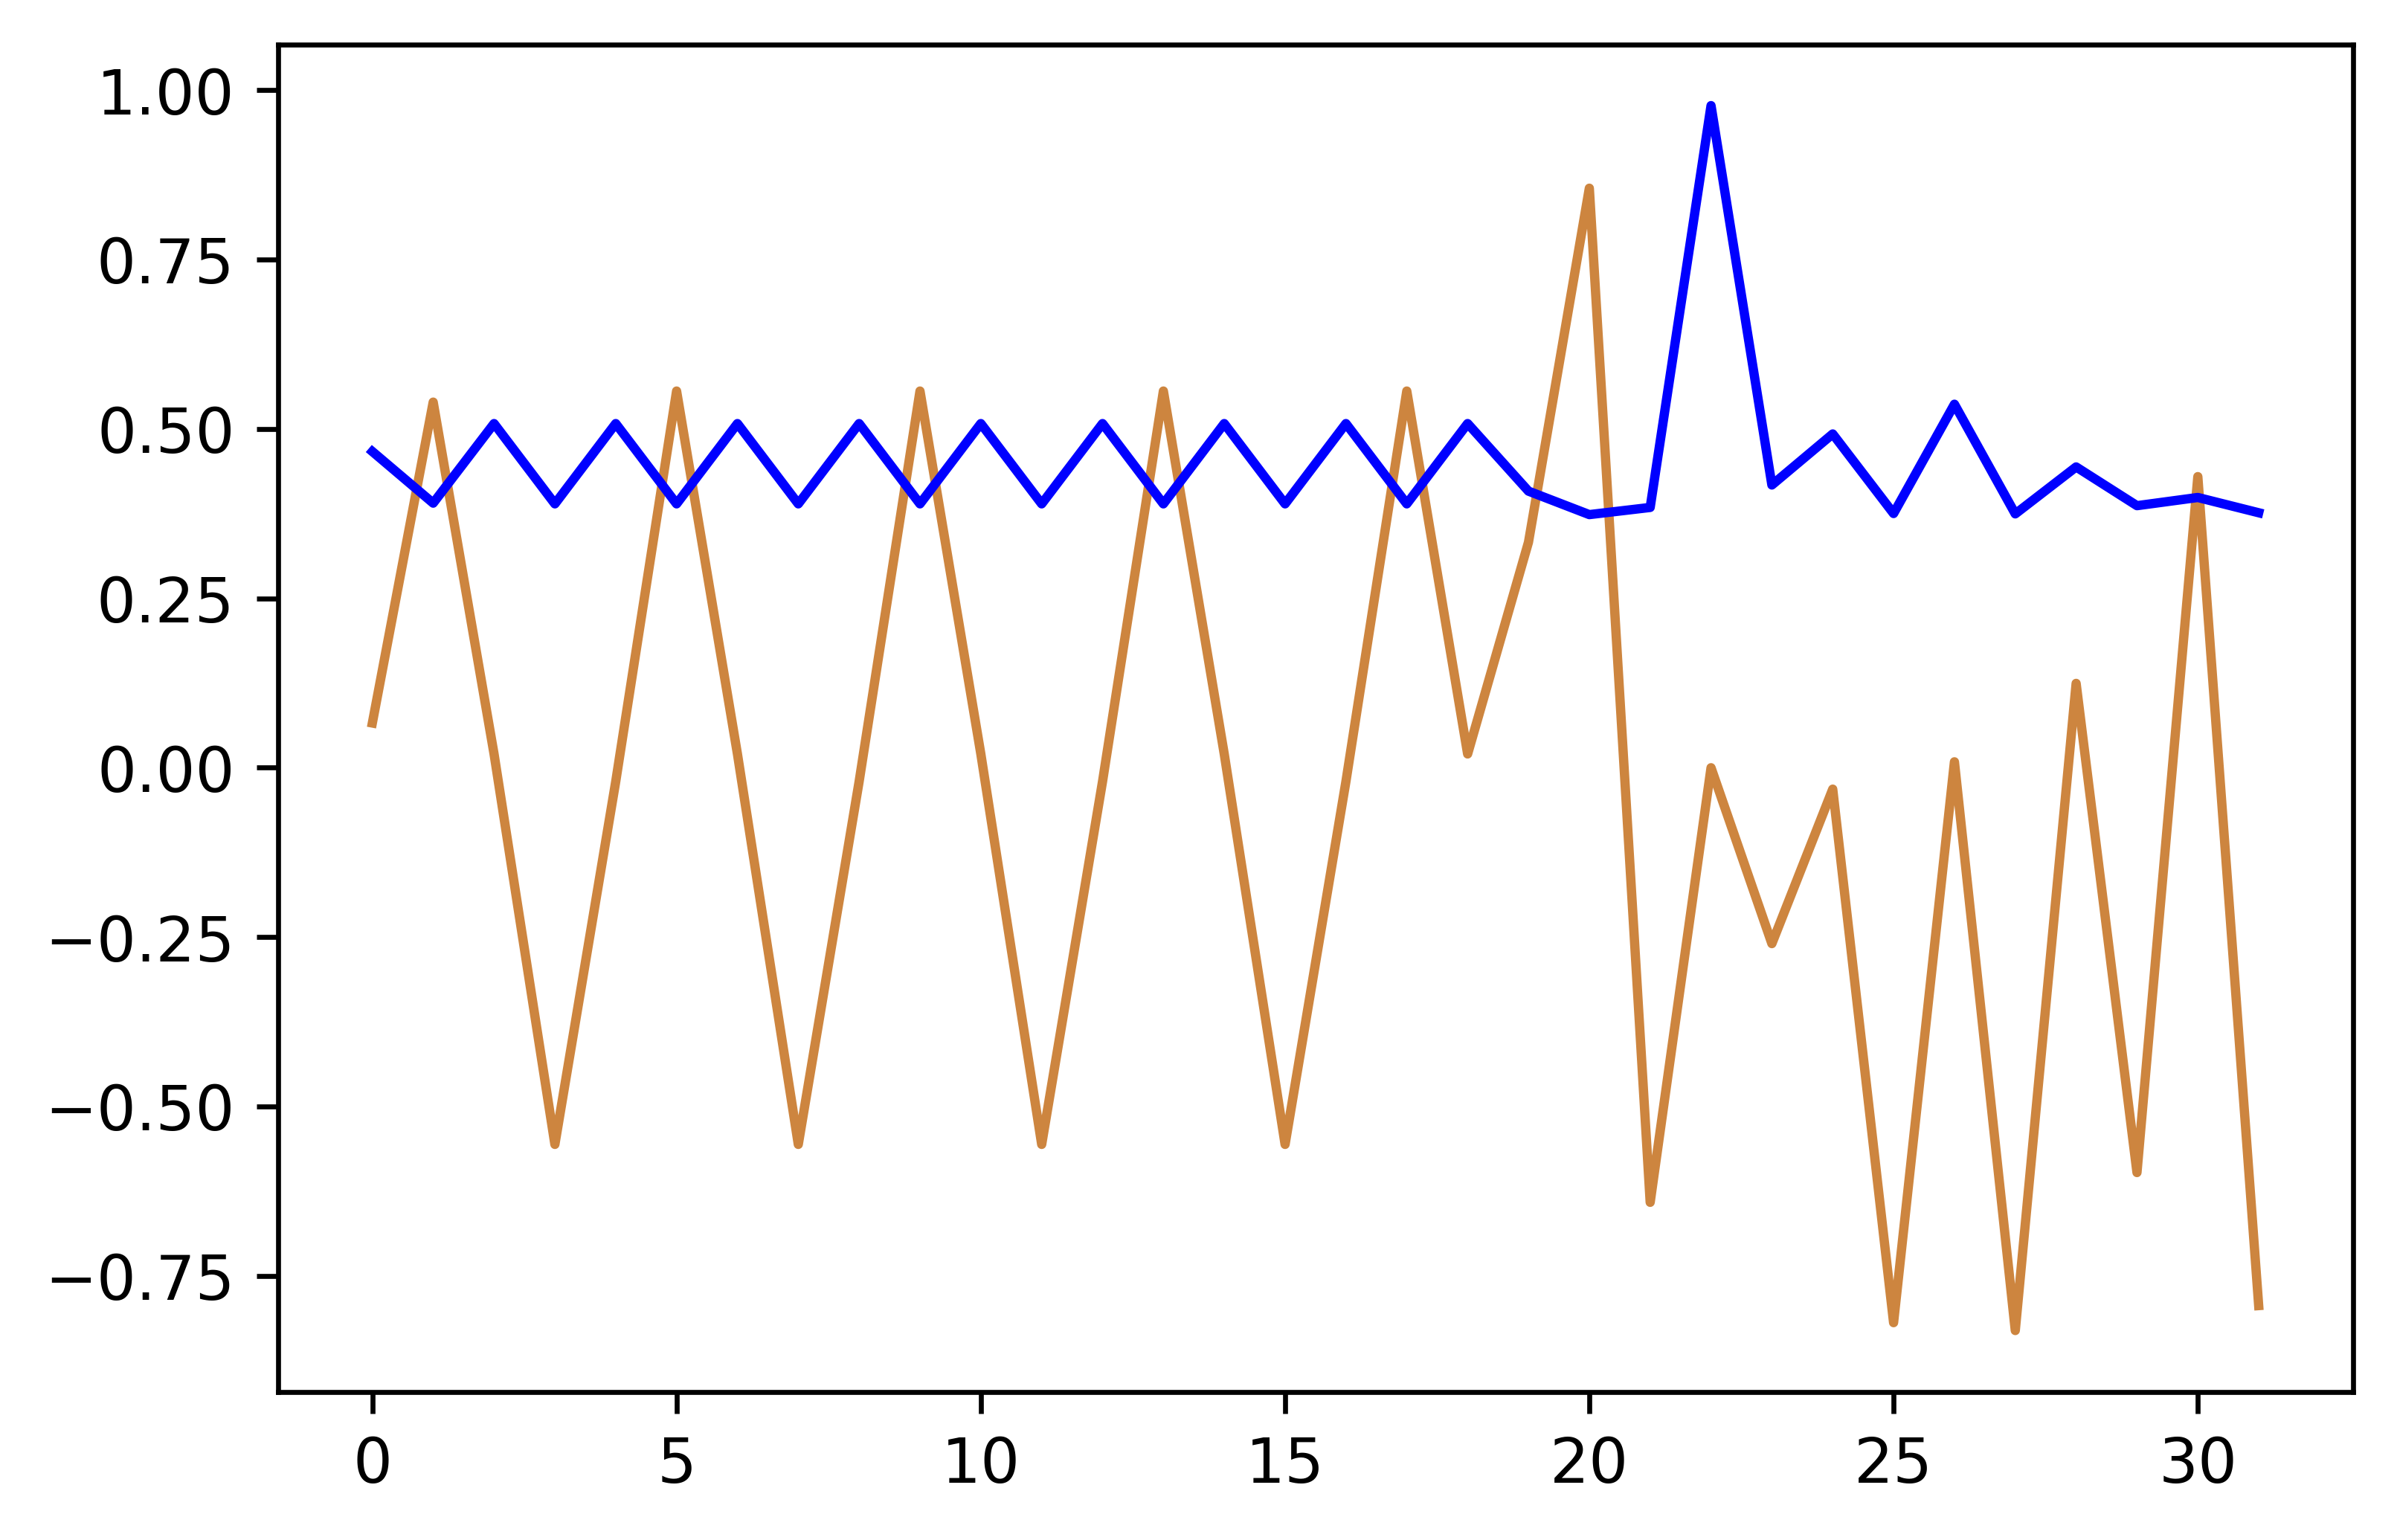
\includegraphics[scale=0.8]{Graphics/example-guido-signal-dst-s.png}
	\caption{DST-II y medida $\mathbb{S}$ usando los las ecuaciones de \textit{matching} \ref{eq:matching-1} \ref{eq:matching-2}} \label{fig:example-guido-signal}
\end{figure}

Usando los filtros anterioes se obitiene el resultado mostrado en la figura \ref{fig:example-guido-signal-dst-s}. 
En este caso la presencia de $m[\cdot]$ se confirma en la posición $22$ de la DST-II y de $\mathbb{S}$, donde se alcanzan valores
cercanos a $0$ y a $1$ respectivamente ($\mathbb{S}=0.9773467949250059$). Este coeficiente corresponde aproximadamente a la posición 
$44$ en la señal original. Como se puede apreciar, existe un ligero desplazamiento en la posición donde se detecta $m[\cdot]$,
pero no es de gran tamaño. De hecho si se toma el coeficiente anterior, la detección es exacta.

\section{Extensión de la DST-II para señales 2D}\label{section:2d}

La DST-II fue diseñada para el caso unidimensional. En este trabajo se busca experimentar sobre las formas en que
este algoritmo se puede extender al caso de señales de bidimensionales. 
En el caso 2D, el patrón $m[\cdot]$ sería en realidad
una matriz $M$ y por tanto se tomarían filas o columnas del mismo para construir la shapelet.
De forma similar la señal $s[\cdot]$ pasa a ser una matriz $X$.
Dado que se está trabajando con imágenes y secciones de las mismas se va a usar de ahora en adelante la notación
$[A:B,C:D]$ para describir una región o porción de la imagen. $A$ y $B$ representan el intervalo en las filas
comprendidos entre dichos valores. De forma similar lo hacen $C$ y $D$, pero para las columnas.
A continuación se exponen algunas ideas sobre la extensión de la DST-II para imágenes y la detección de patrones en este tipo de señales.

\subsection{Primer enfoque: DST-II por filas y luego columnas}

La DST-II comparte muchas de las características de la DWT. Ambas transformadas se pueden obtener a través del
algoritmo de Mallat. Por este motivo una primera idea para extender la DWT-II para señales de dos dimensiones
es usar la descomposición no estándar descrita en \ref{section:dwt-2d}.
Como resultado de la misma se obtendrían cuatro componentes. 

Los coeficientes de aproximación no son de interés para la detección. Nótese que la DST-II realizaba la detección en la sección
\textit{second-rated}, que corresponde a los coeficientes de detalles en la DWT. Por tanto, solo se analizaran para
la detección las componentes LH,HL y HH.
En este enfoque, sea $X$ la señal de entrada (imagen) con dimensiones $n\times m$, entonces al realizar el algoritmo de descomposición estándar
cada una de los componentes tiene dimensiones $n/2 \times m/2$. Luego, sea $c_{i,j}$ un coeficiente
ubicado en la fila $i$ y la columna de $j$ de cualquiera de las componentes, el mismo corresponde
a la posición $(2i,2j)$ de $X$.

\subsection{Segundo enfoque: DST-II solamente por filas (columnas)}

Dado que el principal objetivo de extender la DST-II para imágenes es aprovechar su capacidad de detección, la cual funciona 
en el caso unidimensional, otra forma de usarla en señales de dos dimensiones es simplemente hacer la transformada
por filas o columnas solamente.
Si se usa este enfoque se pueden tomar secciones horizontales y verticales del patrón que se quiere detectar para 
la construcción de las shapelets y obtener información en filas y columnas.

Sea $X$ la imagen de entrada de dimensiones $n\times m$, entonces si la DST-II se hace por filas se obtiene
como resultado otra imagen de dimensiones $n \times m/2$. De forma análoga si se hace por columnas, se obtiene
una imagen con dimensiones $n/2 \times m$. Nótese que se está asumiendo que se toma solamente la 
\textit{second-rated} de la DST-II. Luego, sea $c_{i,j}$ el coeficiente $i$ de la \textit{second-rated} 
de la DST-II sobre la fila $i$ , si esta última se hace por filas
entonces el coeficiente corresponde a la fila $j$ y la columna $2j$ en $X$. De forma análoga si se hace
la DST-II por columnas, el coeficiente $c_{i,j}$ corresponde a la fila $2i$ y a la columna $j$.

\subsection{Tercer enfoque: DST-II usando varias shapelets}

Dado que mientras más \textit{shapelet} construidas a partir de distintas secciones del patrón pueden brindar más información
sobre su localización, entonces se propone como otra alternativa el mismo enfoque anterior, pero construyendo
varias \textit{shapelets} a partir de distintas secciones del patrón que se quiere detectar. Luego, los resultados
de cada una de las transformadas sobre la señal $X$ se promedian. Con esta técnica lo que se buscar es lograr definir
el contorno donde se detectan las distintas partes del patrón.

\chapter{Experimentos}\label{chapter:implementation}

En el capítulo anterior se expuso cómo se construyen los filtros de la DST-II, la metodología para
la detección usando este algoritmo y algunas ideas para su extensión a señales de dos dimensiones. Con esta información,
ya es posible pasar a la parte de los experimentos. 
En este capítulo se presenta y describe cada uno de los experimentos que se llevó a cabo para evaluar el rendimiento 
del algoritmo de la DST-II en la detección de patrones y para explorar la factibilidad de las propuestas
para el caso 2D en señales artificiales y en la detección de masas en mamografías.

\section{Consideraciones generales de la etapa de experimentación}

La implementación se realizó en Python 3 \cite{python3} haciendo uso de los paquetes Sympy \cite{10.7717/peerj-cs.103}, 
Scipy \cite{2020SciPy-NMeth}, scikit-learn \cite{sklearn_api}, scikit-image \cite{van2014scikit},
Pydicom \cite{darcy_mason_2020_4313150}
y PyWavelets \cite{Lee2019}. Todos los experimentos se 
realizaron en Jupyter Notebooks \cite{Kluyver2016jupyter} y al igual que la DST-II están disponibles en el repositorio de
\href{https://github.com/adrian13579/discrete-shapelet-transform}{GitHub} correspondiente a esta tesis.

El equipo de cómputo donde se realizaron los experimentos posee las siguientes propiedades:

\begin{itemize}
	\item Memoria: 8.0 GB
	\item Procesador: Intel® Core™ i3-8130U CPU @ 2.20GHz × 4
	\item Arquitectura: 64-bit
\end{itemize}


\section{Solución numérica del sistema de ecuaciones no lineales}

En la sección \ref{numerical-solution} se mencionan algunos de los métodos usados para solucionar sistemas de 
ecuaciones no lineales. Los siguientes experimentos tienen como objetivo evaluar dichos métodos en la solución
del sistema de ecuaciones para obtener el filtro $q[\cdot]$ de la DST-II.

\subsection{Ejemplos de los experimentos y análisis de los resultados}

Para comprobar la eficiencia de los métodos numéricos seleccionados se utilizó un dataset formado por 85 patrones, con longitudes de entre $9$ y 
$29$ muestras, con amplitudes desde $-10$ hasta $10$.

Para calcular el error de las soluciones se evaluaron en cada una de las ecuaciones del sistema. Como resultado
se obtiene el error residual de la solución para cada ecuación. Para tener una medida del error total
de la solución, se tomó el valor absoluto de cada uno de estos residuos y se sumaron.

\begin{table}
	\centering
	\caption{Tiempo y error promedio de los métodos numéricos usados.} \label{table:numerical-error}
	\begin{tabular}{|c|c|c|} \toprule
		Método numérico  & Tiempo promedio (segundos) & Error promedio \\ \midrule 
		lm & 19.96 & 0.20 \\ 
		hybr & 2.62 & 0.50 \\
		broyden1 & 79.02 & 2.86$\times 10^{53}$\\
		broyden2 & 78.91 & 2.86$\times 10^{53}$\\
		krylov & 183.51 & 4249.50 \\
		anderson & 57.28 & 3.59$\times 10^{26}$\\ \bottomrule
	\end{tabular}
\end{table}

La Tabla \ref{table:numerical-error} muestra el resultado del experimento. Se puede apreciar que los métodos 
con un error promedio aceptable son el de Levenberg-Marquardt (lm) y el Método Híbrido de Powell (hybr). 
Siendo el error del primer algoritmo menor.
En el caso del tiempo, Levenberg-Marquardt y el Método Híbrido de Powell fueron los más rápidos. Aún así, la
diferencia entre este último y Levenberg-Marquardt es poca en comparación con el resto de los métodos.

\begin{table}
	\centering
	\caption{Por ciento de casos donde se alcanzó la convergencia según el método numérico.} \label{table:numerical-convergence}
	\begin{tabular}{|c|c|c|} \toprule
		Método numérico & Convergencia (\%)\\ \midrule
		lm & 0.72 \\
		hybr & 0.26 \\
		broyden1 & 0.11 \\
		broyden2 & 0.11 \\
		krylov & 0.00 \\
		anderson & 0.09 \\ \bottomrule
	\end{tabular}
\end{table}

Los resultados sobre la convergencia se muestran en la Tabla \ref{table:numerical-convergence}. Se puede
observar que Levenberg-Marquardt fue el que alcanzó la convergencia en la mayoría de los casos, seguido 
por hybr. En el caso de Krylov, no logró la convergencia en ninguno de los casos.

\section{Detección de patrones en señales 1D}

En esta sección se presentan algunos experimentos realizado para evaluar la capacidad  de detección de la replicación
del algoritmo de la DST-II.

Para los experimentos se tomaron un conjunto de señales con una longitud máxima de 200 muestras, y luego
se insertaron patrones en distintas posiciones de forma aleatoria en cada corrida del experimento. En cada señal 
se inserta solamente un patrón. Las señales seleccionadas se encuentran en PyWavelets
y son las siguientes:

Blocks, Bumps, HeaviSine, Doppler, Ramp, TwoChirp, QuadChirp, MishMash, WernerSorrows, HypChirps, LinChirps, Chirps y sineoneoverx.

Los patrones usados se encuentran en el repositorio y fueron generados a mano tratando de imitar señales biomédicas que
aparecen en \cite{Guido2018}. El tamaño de los patrones es entre 14 y 27 muestras.

Las métricas usadas para analizar los resultados de los experimentos fueron:

\begin{itemize}
	\item Matriz de confusión: Cada fila de la matriz presenta instancias de la clase real, mientras que cada columna instancias
		de la clase que se predice, o vice versa \cite{CIFUENTES2010}.
	\item Curva ROC: La curva ROC (\textit{receiver operating characteristic curve}) es un gráfico que muestra la habilidad de diagnosticar
		de un clasificador binario. La curva se crea ploteando el TPR (\textit{true positive rate}) con el FPR (\textit{false positive rate})
		\cite{CERDA2012}.
	\item Histograma: Gráfico usado para la distribución de frecuencias. 
\end{itemize}

Como criterio de detección se usa la medida $\mathbb{S}$ sobre la sección \textit{second-rated} de la
DST-II y un umbral $th$ sobre la misma. Es decir, para cualquier coeficiente $c$, tal que $\mathbb{S}(c)\geq th$, se considera
que se detectó la señal en la posición correspondiente al coeficiente $c$. Si ningún coeficiente cumple la condición
anterior se considera que el algoritmo no detecta el patrón dentro de la señal. 

En el caso de la curva ROC, se comparan también los resultados con el de otras wavelets. En el caso de estas
últimas se usó la misma medida, pero sobre los coeficientes de detalle. De este modo, se busca evaluar 
la capacidad del algoritmo de la DST-II para detectar patrones.

Los histogramas son usados para mostrar la frecuencia de los valores correspondientes a la diferencia entre
la posición donde se encuentra realmente el patrón dentro de la señal y la posición que predice el algoritmo.
Valores negativos indican que se detectó antes, y valores positivos que se detectó después.

\subsection{Ejemplos de los experimentos y análisis de los resultados}

Las figuras \ref{fig:cm-comparison}, \ref{fig:roc-comparison} y \ref{fig:hist-comparison} 
muestran los resultados de la DST-II en la detección en tres escenarios distintos.
Primero, con un grupo de patrones de entre 15 y 27 muestras, y luego con patrones de 19 y 27 
muestras, respectivamente. En el caso del experimento con varios patrones se observa que 
la \textit{shapelet} es capaz de reaccionar ante la presencia de los patrones insertados en las señales en 
la mayoría de los casos. En la Figura \ref{fig:roc-comparison} se observa que la \textit{shapelet}
es superior a las demás wavelets en la detección. Sin embargo, el tamaño del patrón es un factor
importante. Nótese que en las figuras \ref{fig:roc-comparison} b) y c) existe una gran diferencia
en los resultados. Esto también se puede observar en la Figura \ref{fig:hist-comparison}, donde 
en el caso del patrón con 27 muestras
la diferencia entre la posición real y la que predice el algoritmo es mayor que en el caso del patrón 
de 19 muestras. Esto se debe a que mientras mayor sea el tamaño del patrón más díficil es resolver
el sistema de ecuaciones no lineales para la construcción del filtro $q[\cdot]$, y, por tanto, el error
de la solución en las condiciones de detección es mayor. Como consecuencia de lo anterior,
la precisión de la DST-II para predecir la posición donde se encuentra el patrón dentro de la señal también
se ve afectada. Las Figura \ref{fig:success-example-experiment} muestra un ejemplo donde la detección
funciona adecuadamente, a difirencia del ejemplo mostrado en la Figura \ref{fig:failed-example-experiment}, donde
el método numérico no logra la convergencia, y como consecuencia, la detección no funciona adecuadamente.

\begin{figure}
	\centering
	\subfigure[Varios patrones de entre 15 y 27 muestras]{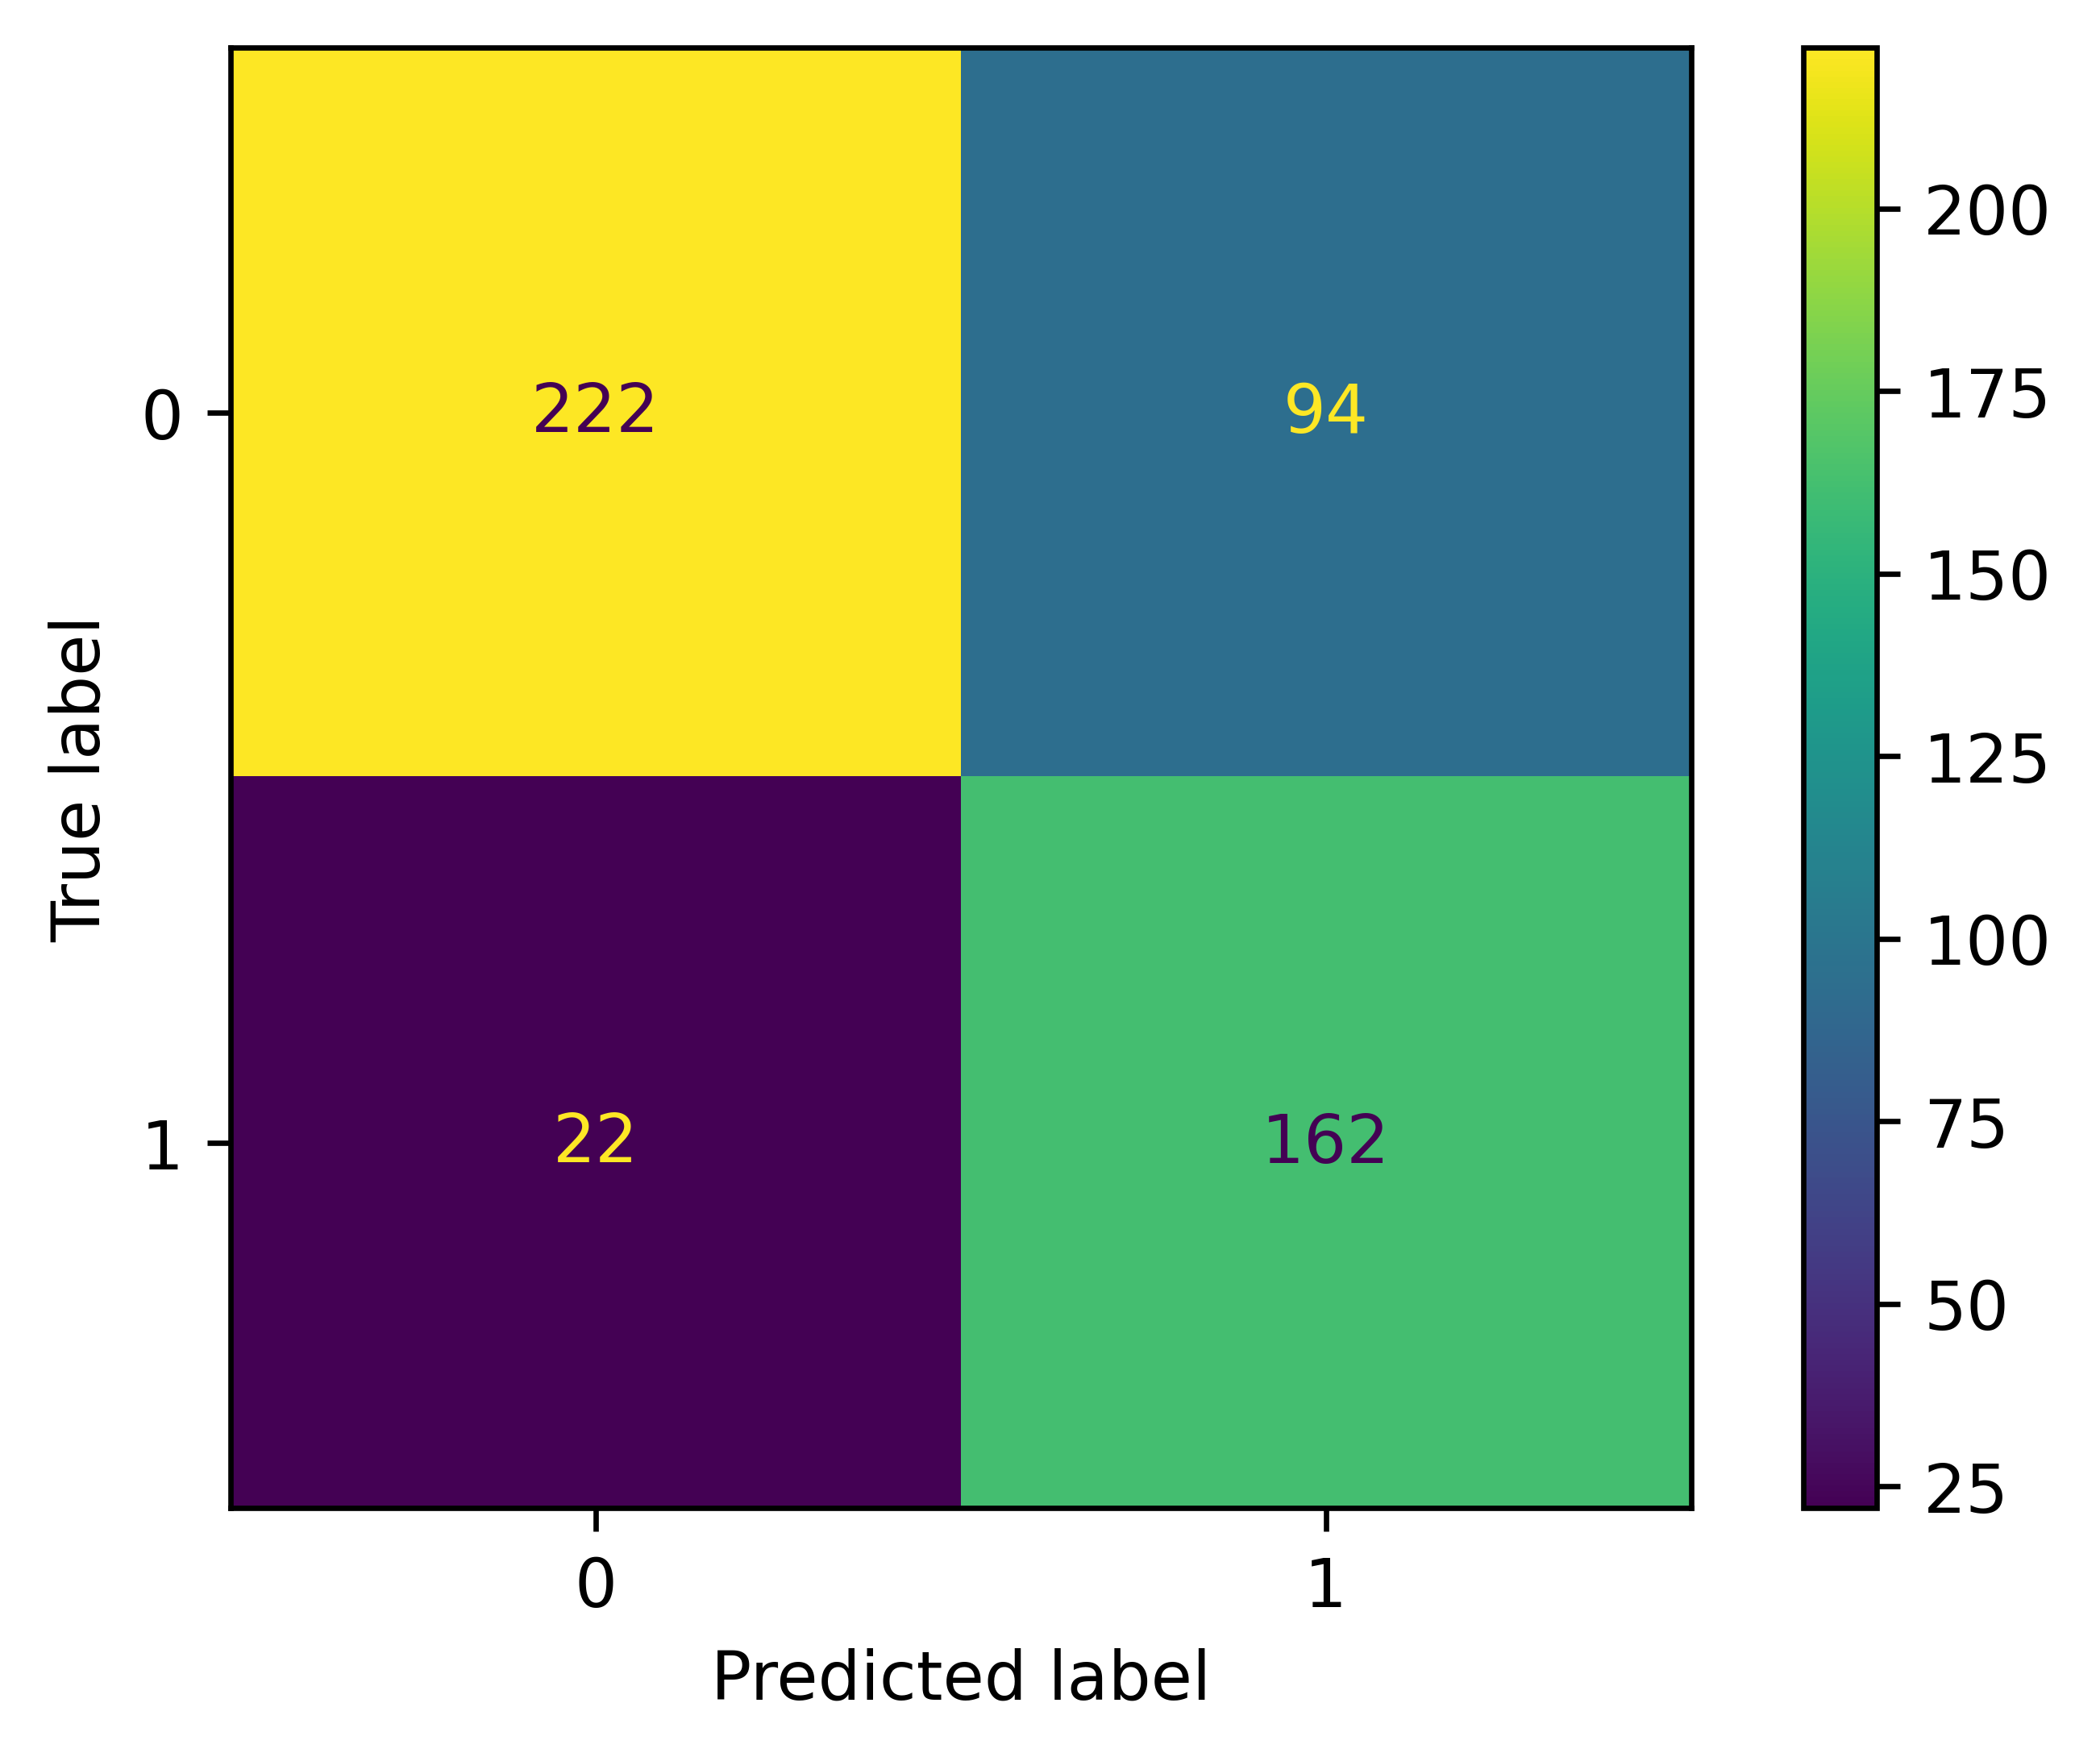
\includegraphics[scale=0.5]{Graphics/cm-th-08-all-patterns.png}}
	\subfigure[Patrón con 27 muestras]{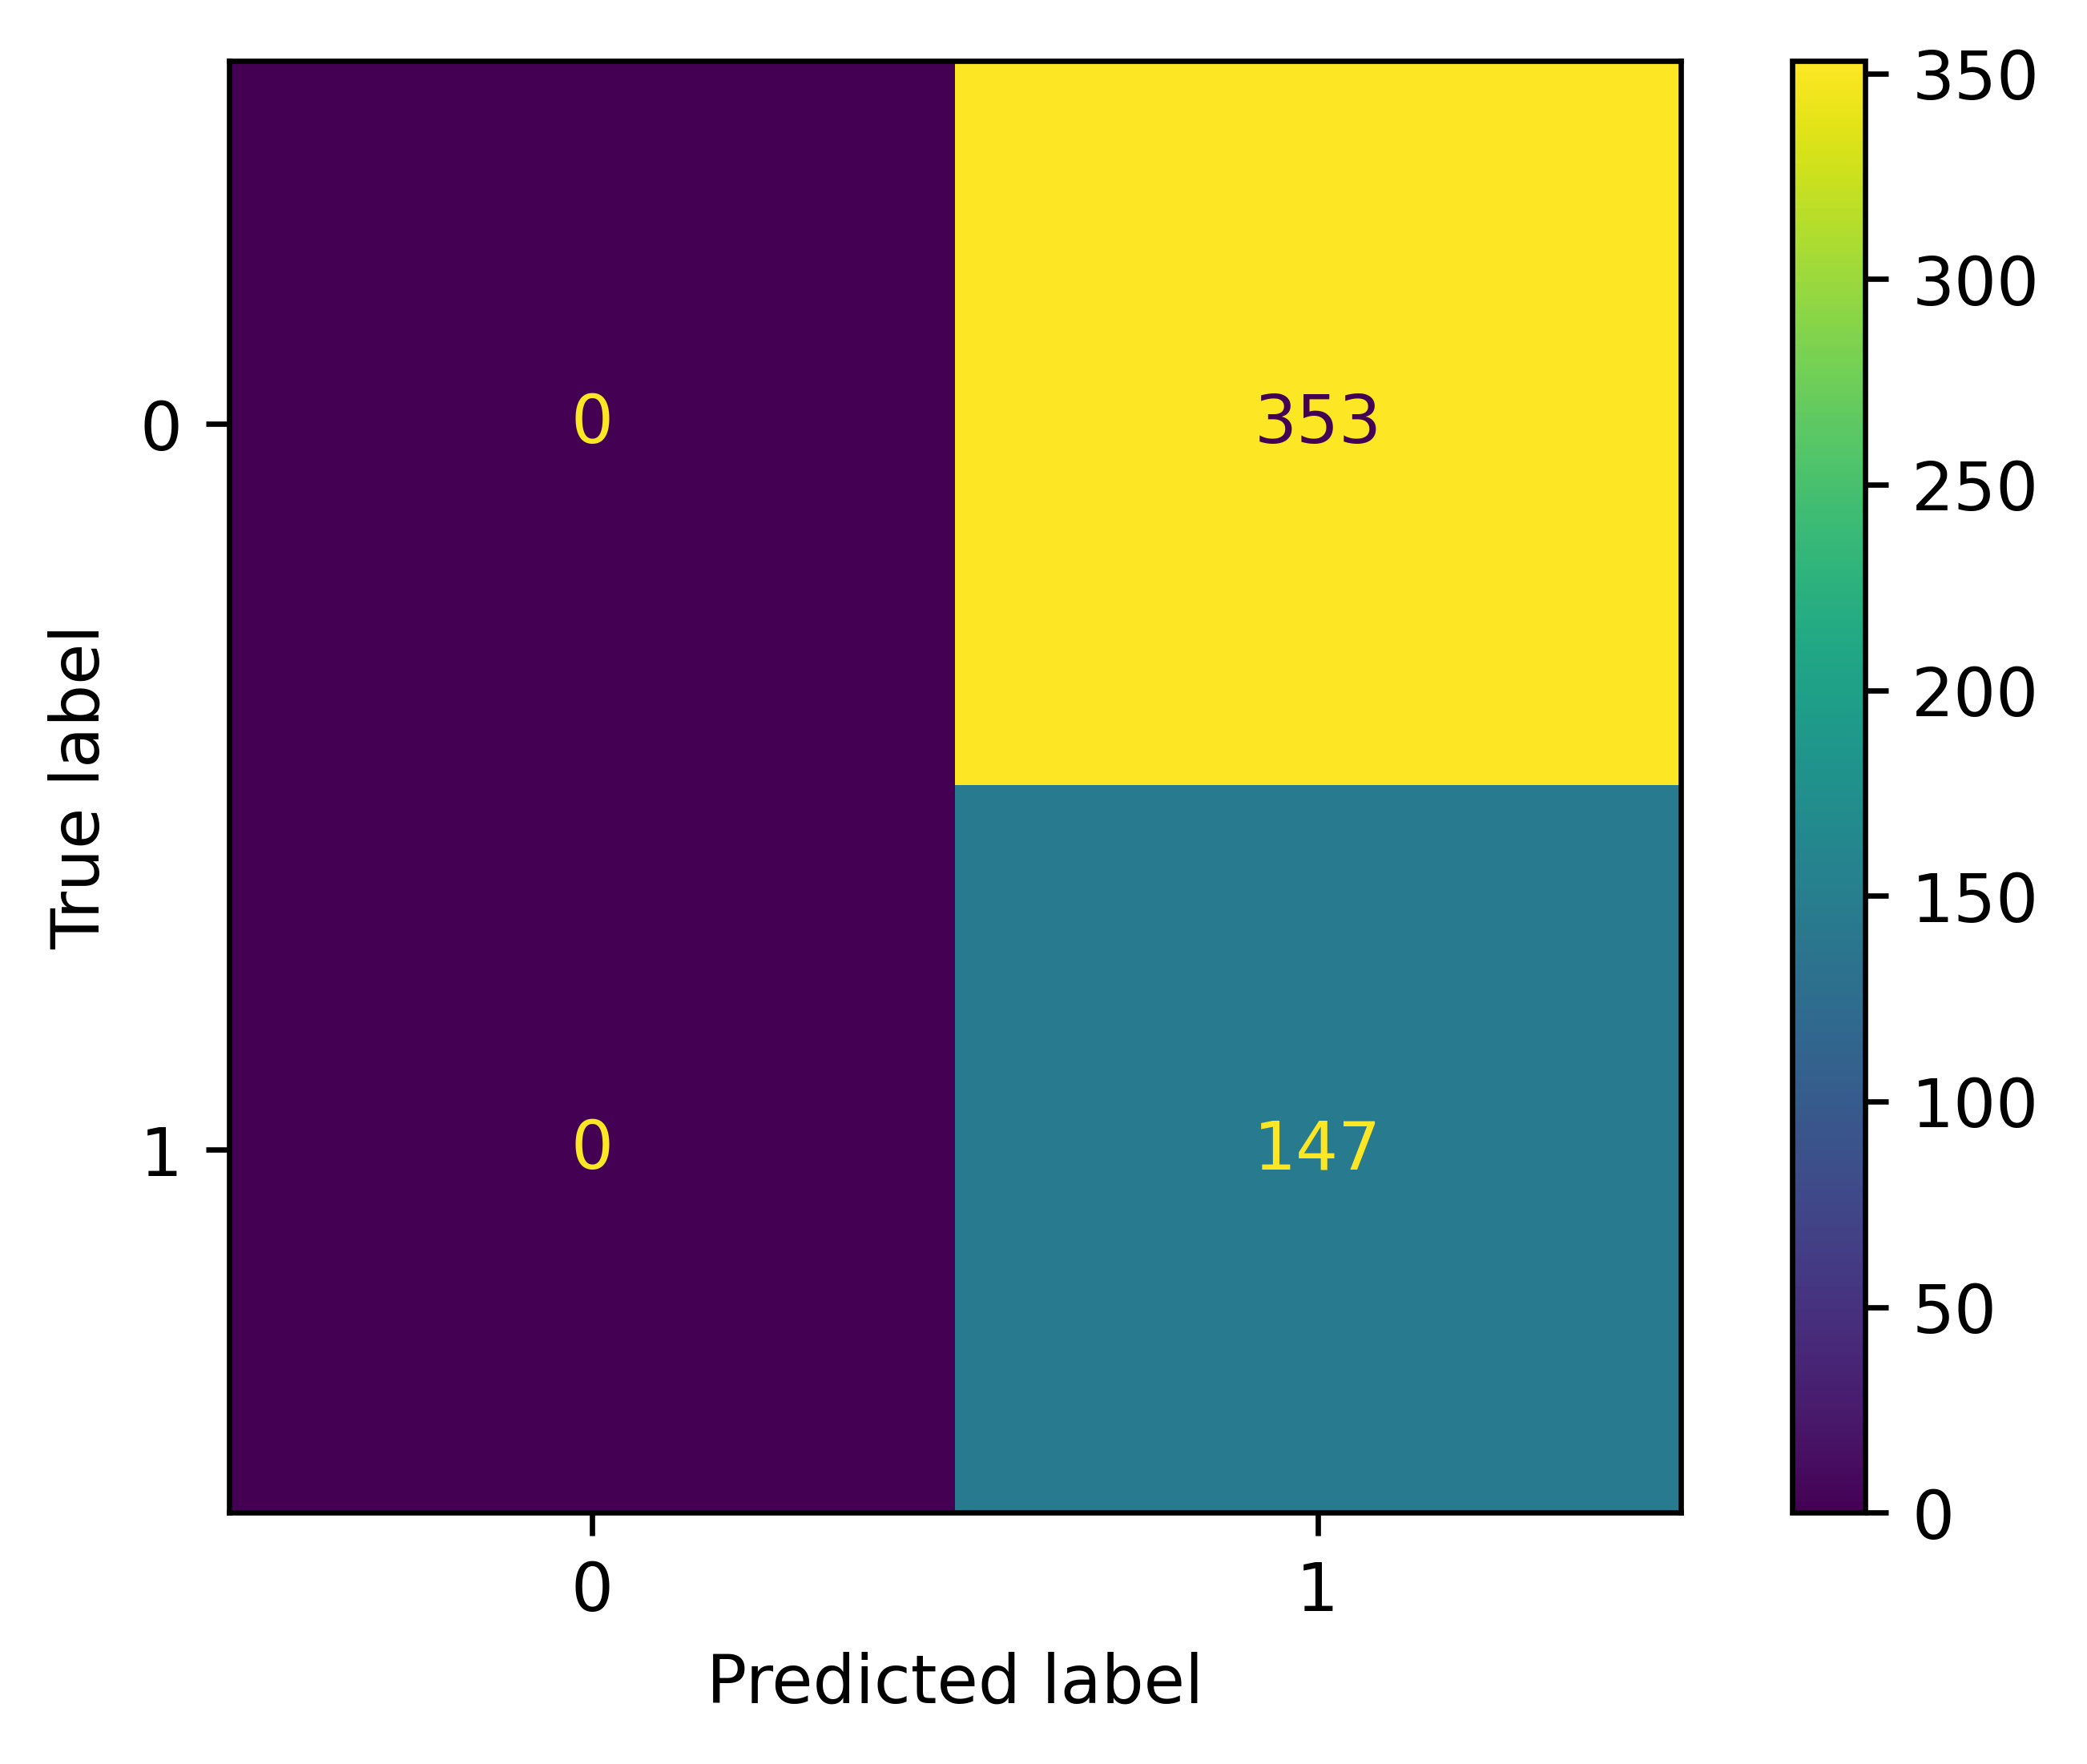
\includegraphics[scale=0.5]{Graphics/cm-th-08-long-pattern.png}}
	\subfigure[Patrón con 19 muestras]{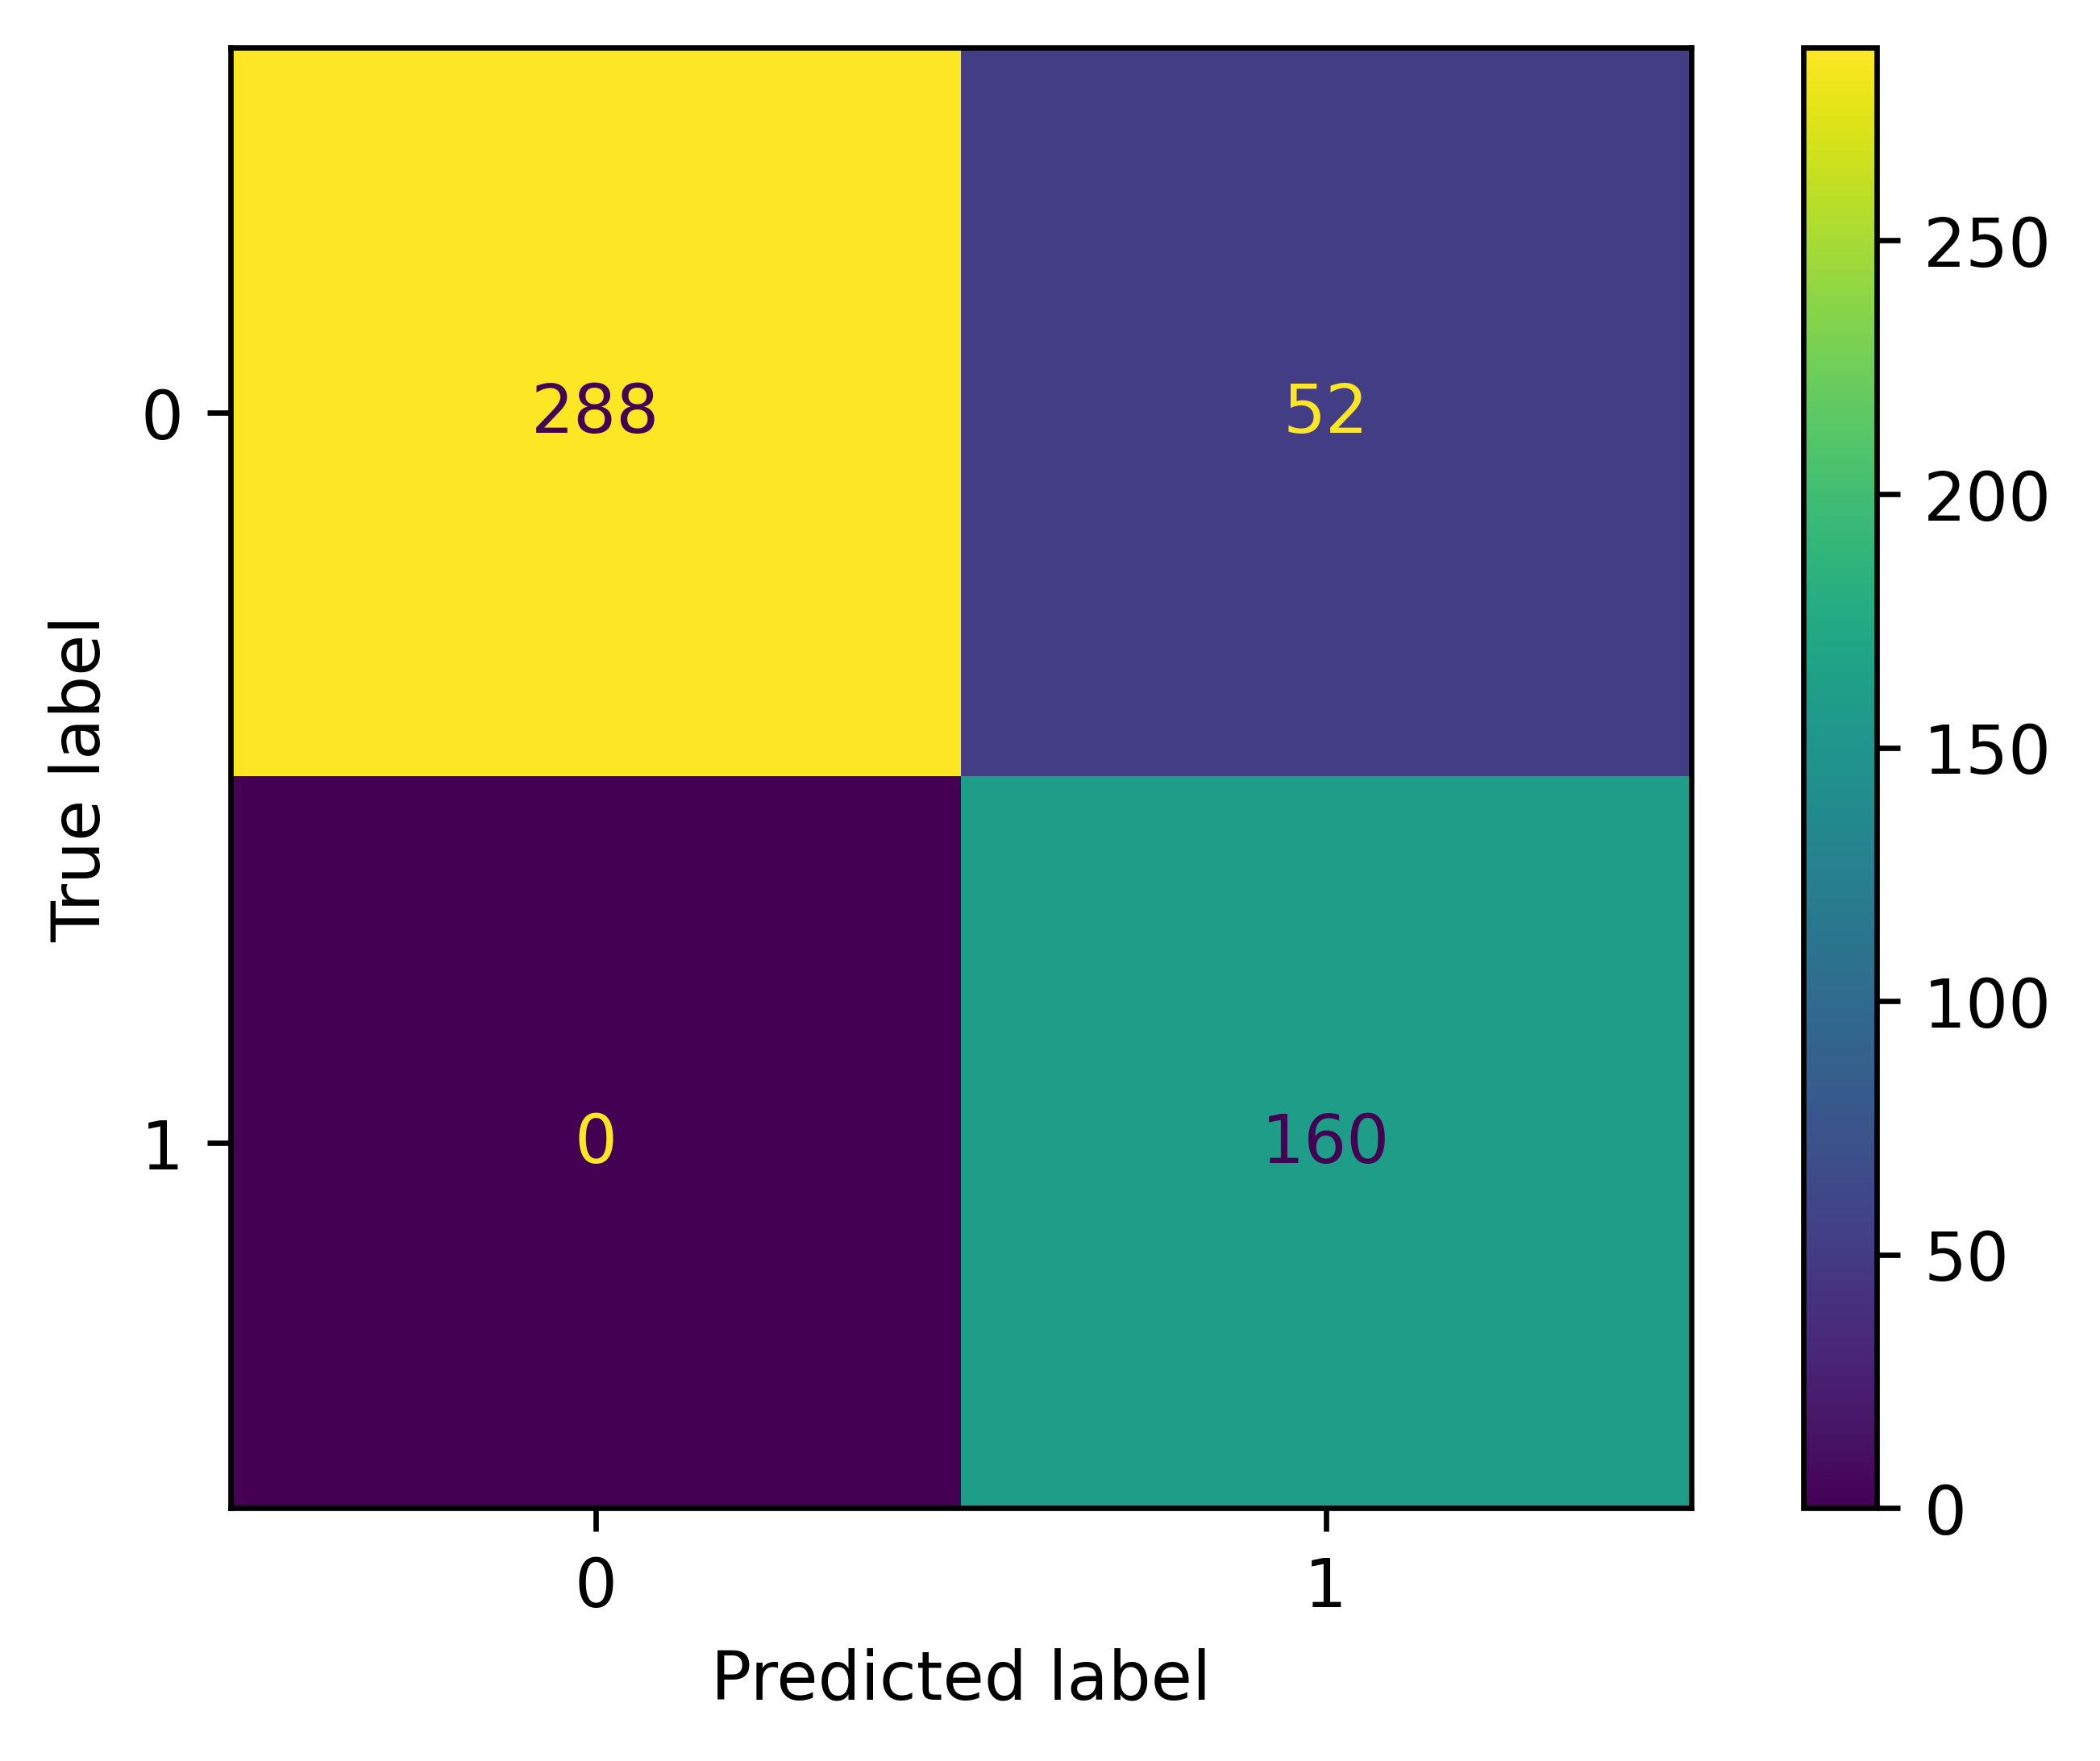
\includegraphics[scale=0.5]{Graphics/cm-th-08-medium-pattern.png}}
	\caption{ Matrices de confusión de cada uno de los experimentos. En todos los casos se usó $th=0.8$.} \label{fig:cm-comparison}
\end{figure} 

\begin{figure}
	\centering
	\subfigure[Varios patrones de entre 15 y 27 muestras]{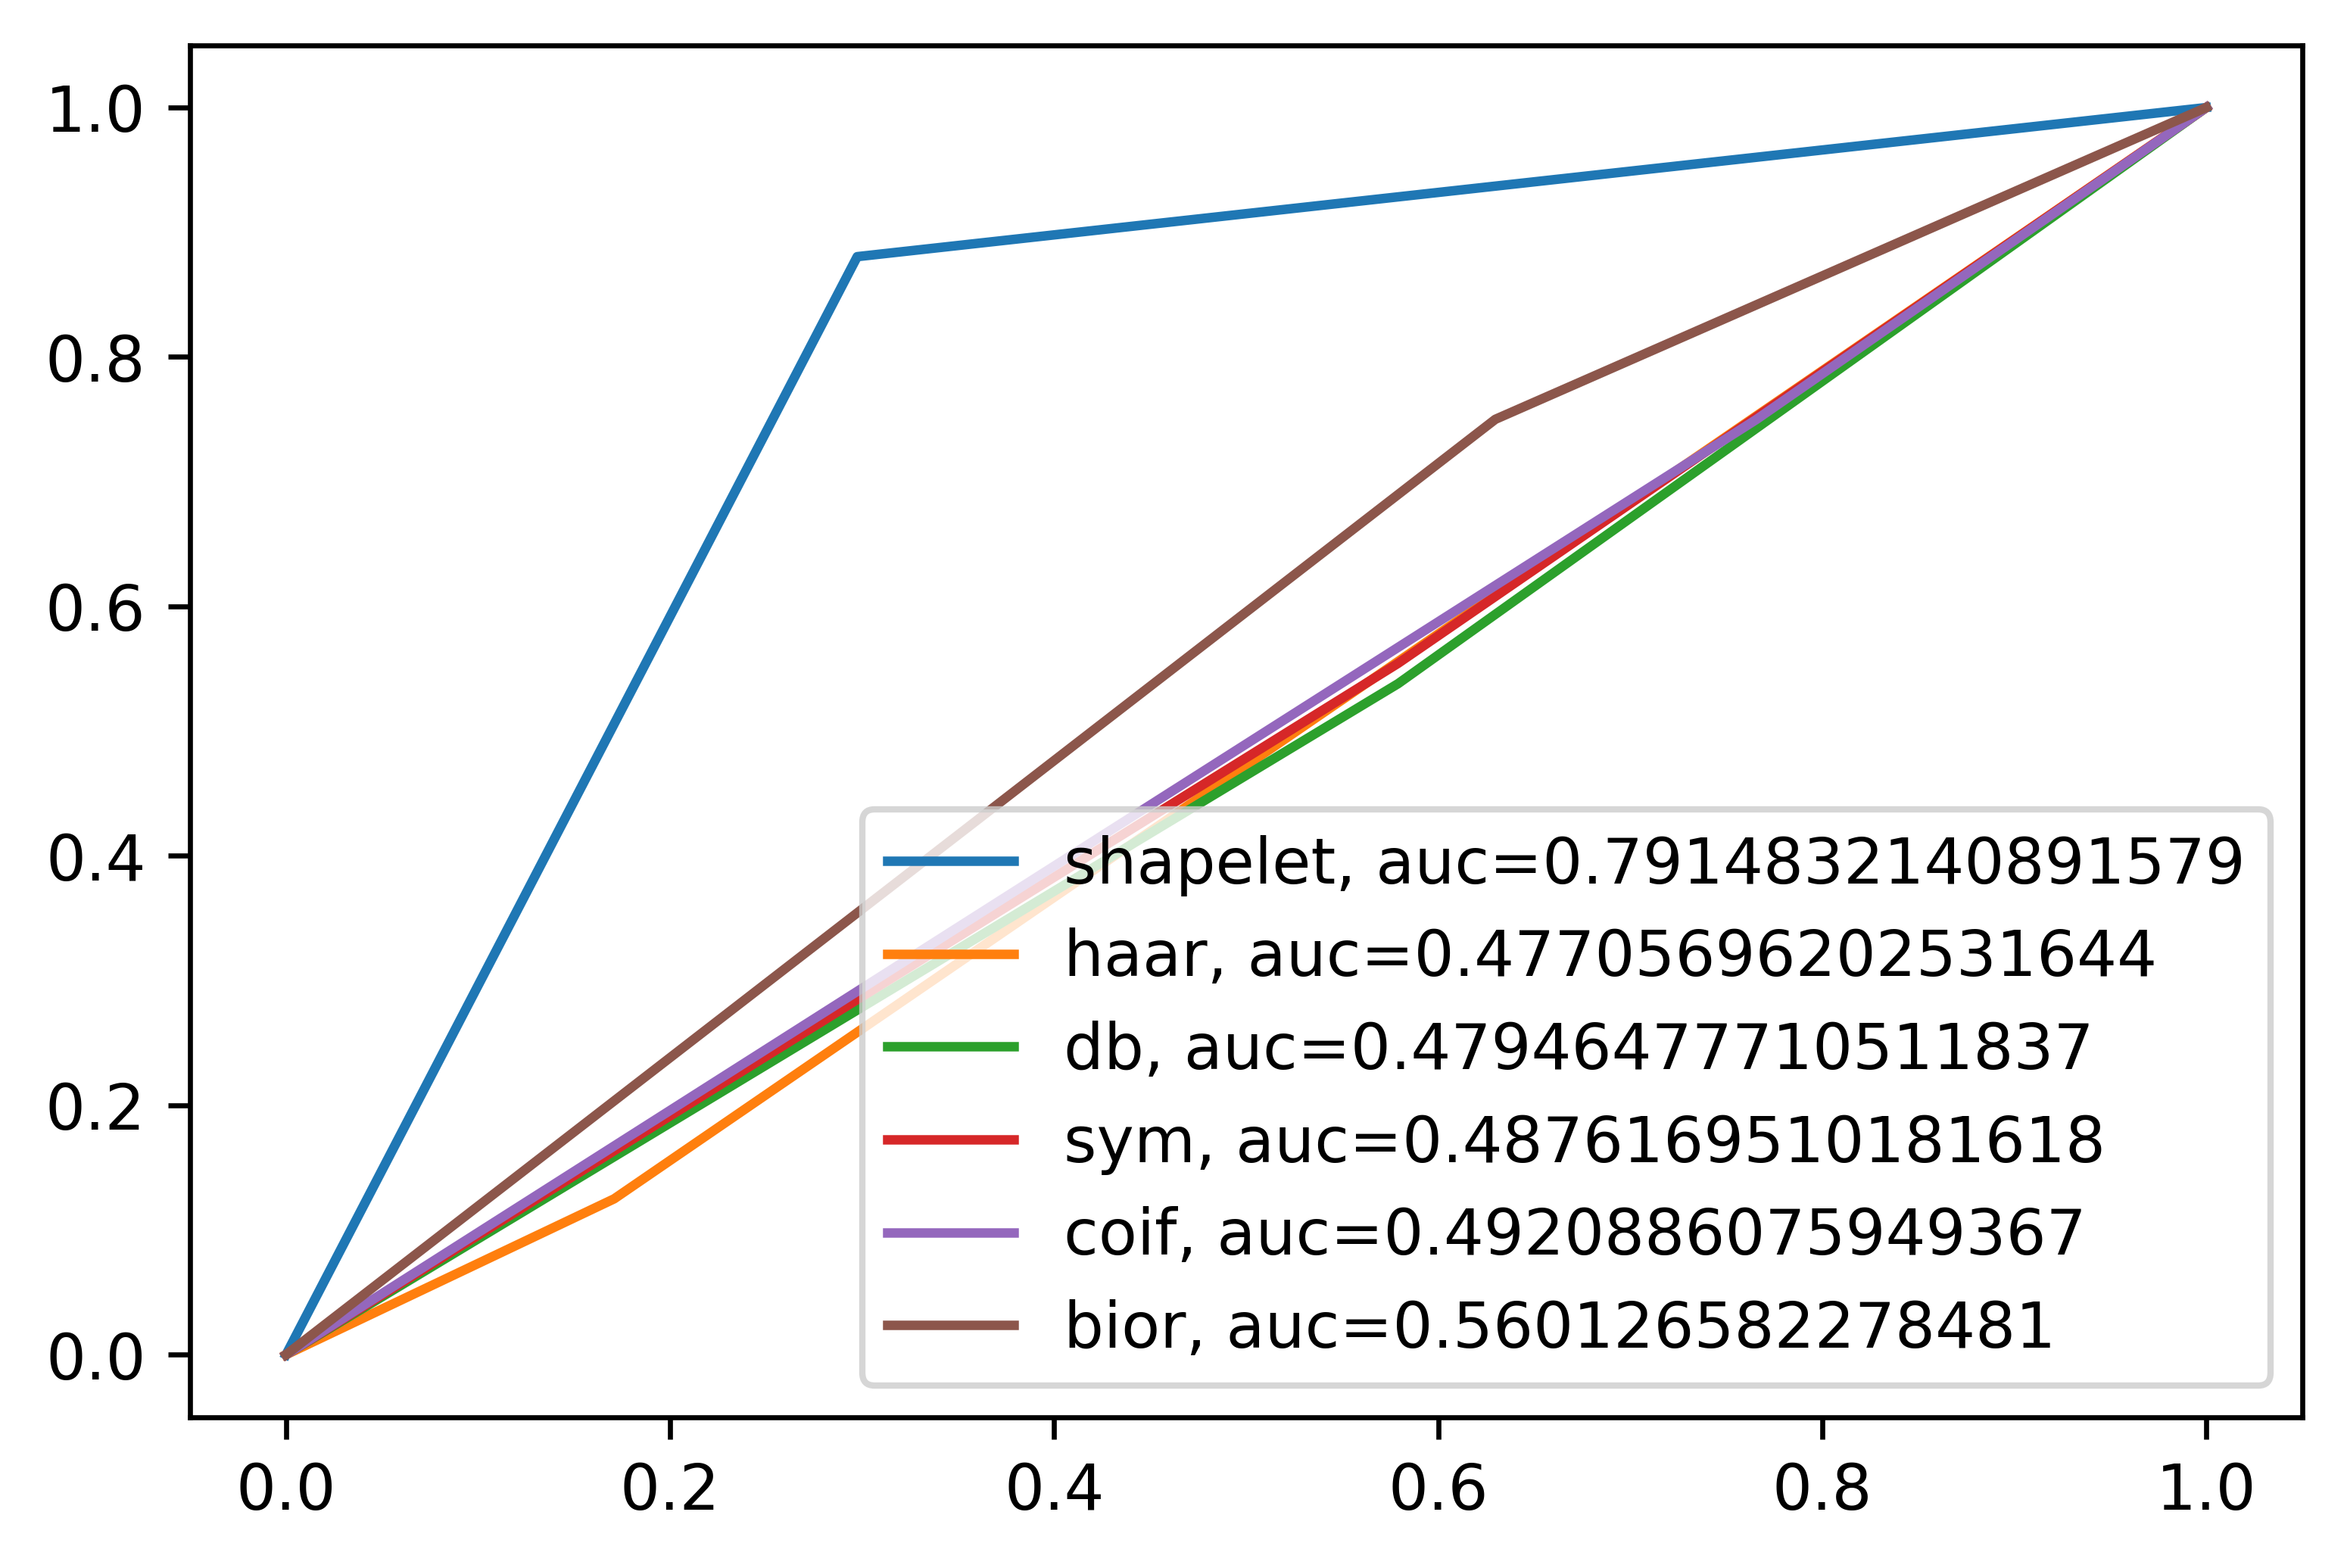
\includegraphics[scale=0.5]{Graphics/roc-th-08-all-patterns.png}}
	\subfigure[Patrón con 27 muestras]{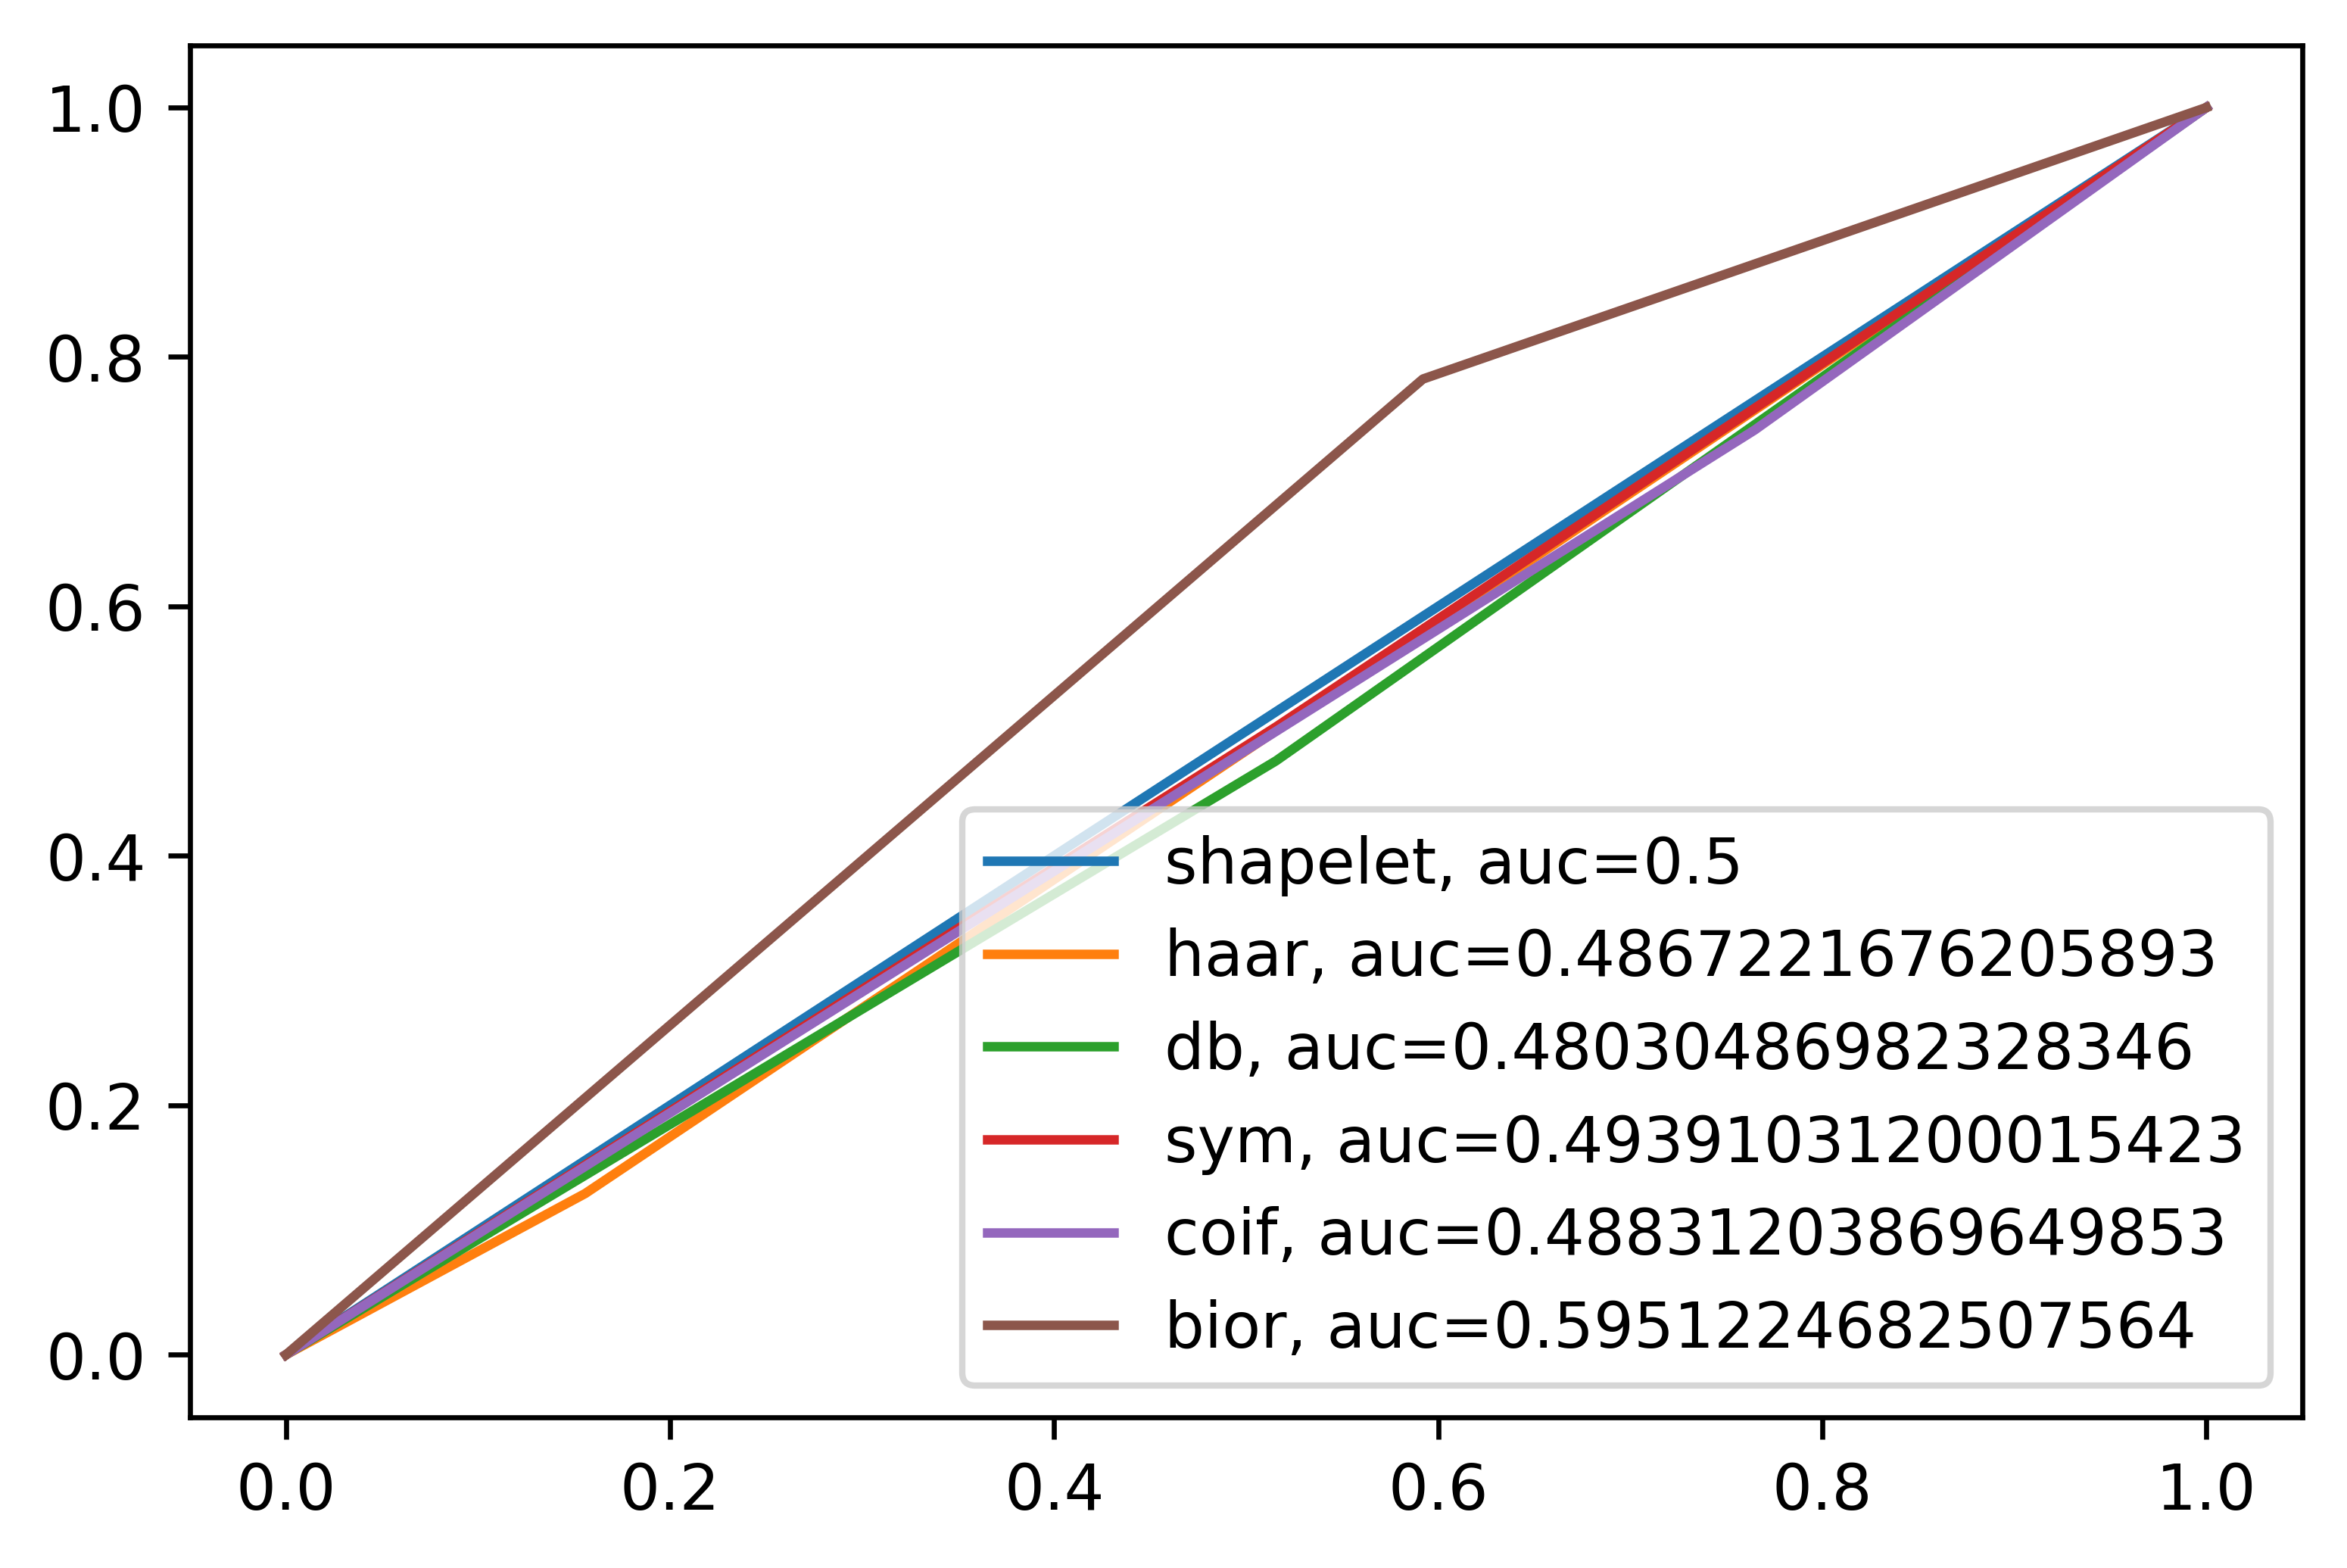
\includegraphics[scale=0.5]{Graphics/roc-th-08-long-pattern.png}}
	\subfigure[Patrón con 19 muestras]{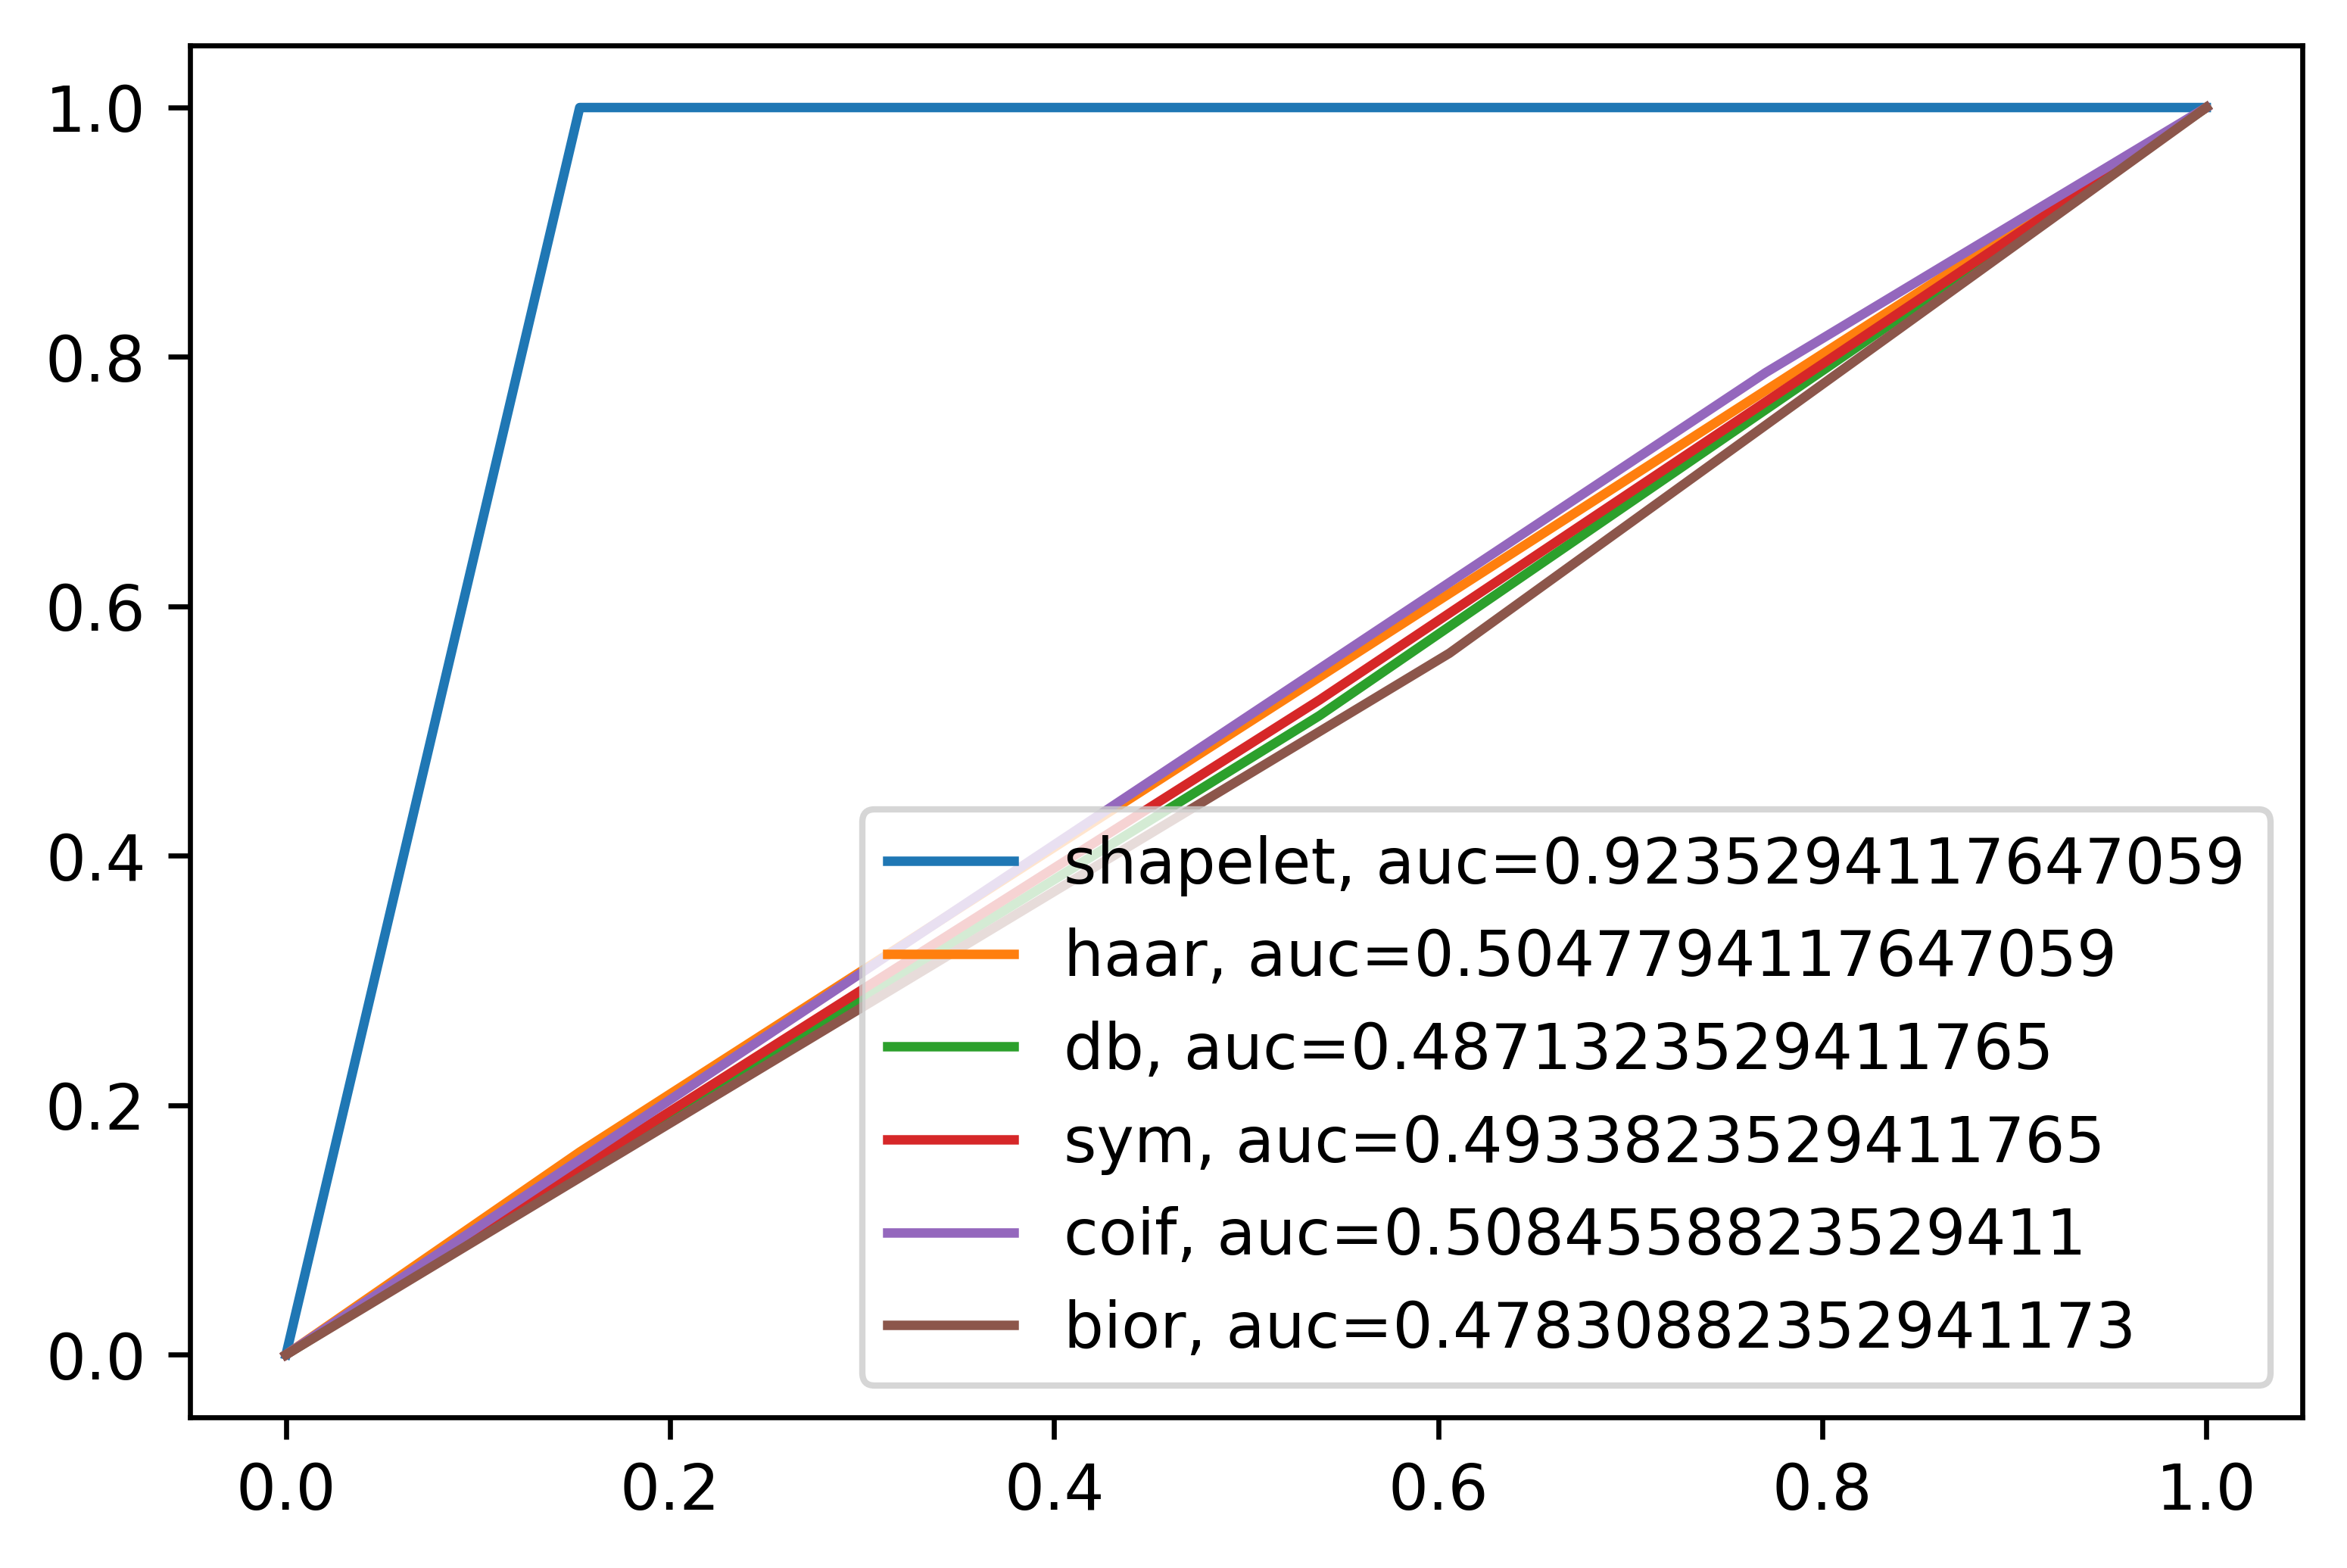
\includegraphics[scale=0.5]{Graphics/roc-th-08-medium-pattern.png}}
	\caption{ Curvas ROC para cada uno de los experimentos. En todos los casos se usó $th=0.8$.} \label{fig:roc-comparison}
\end{figure} 

\begin{figure}
	\centering
	\subfigure[Varios patrones de entre 15 y 27 muestras]{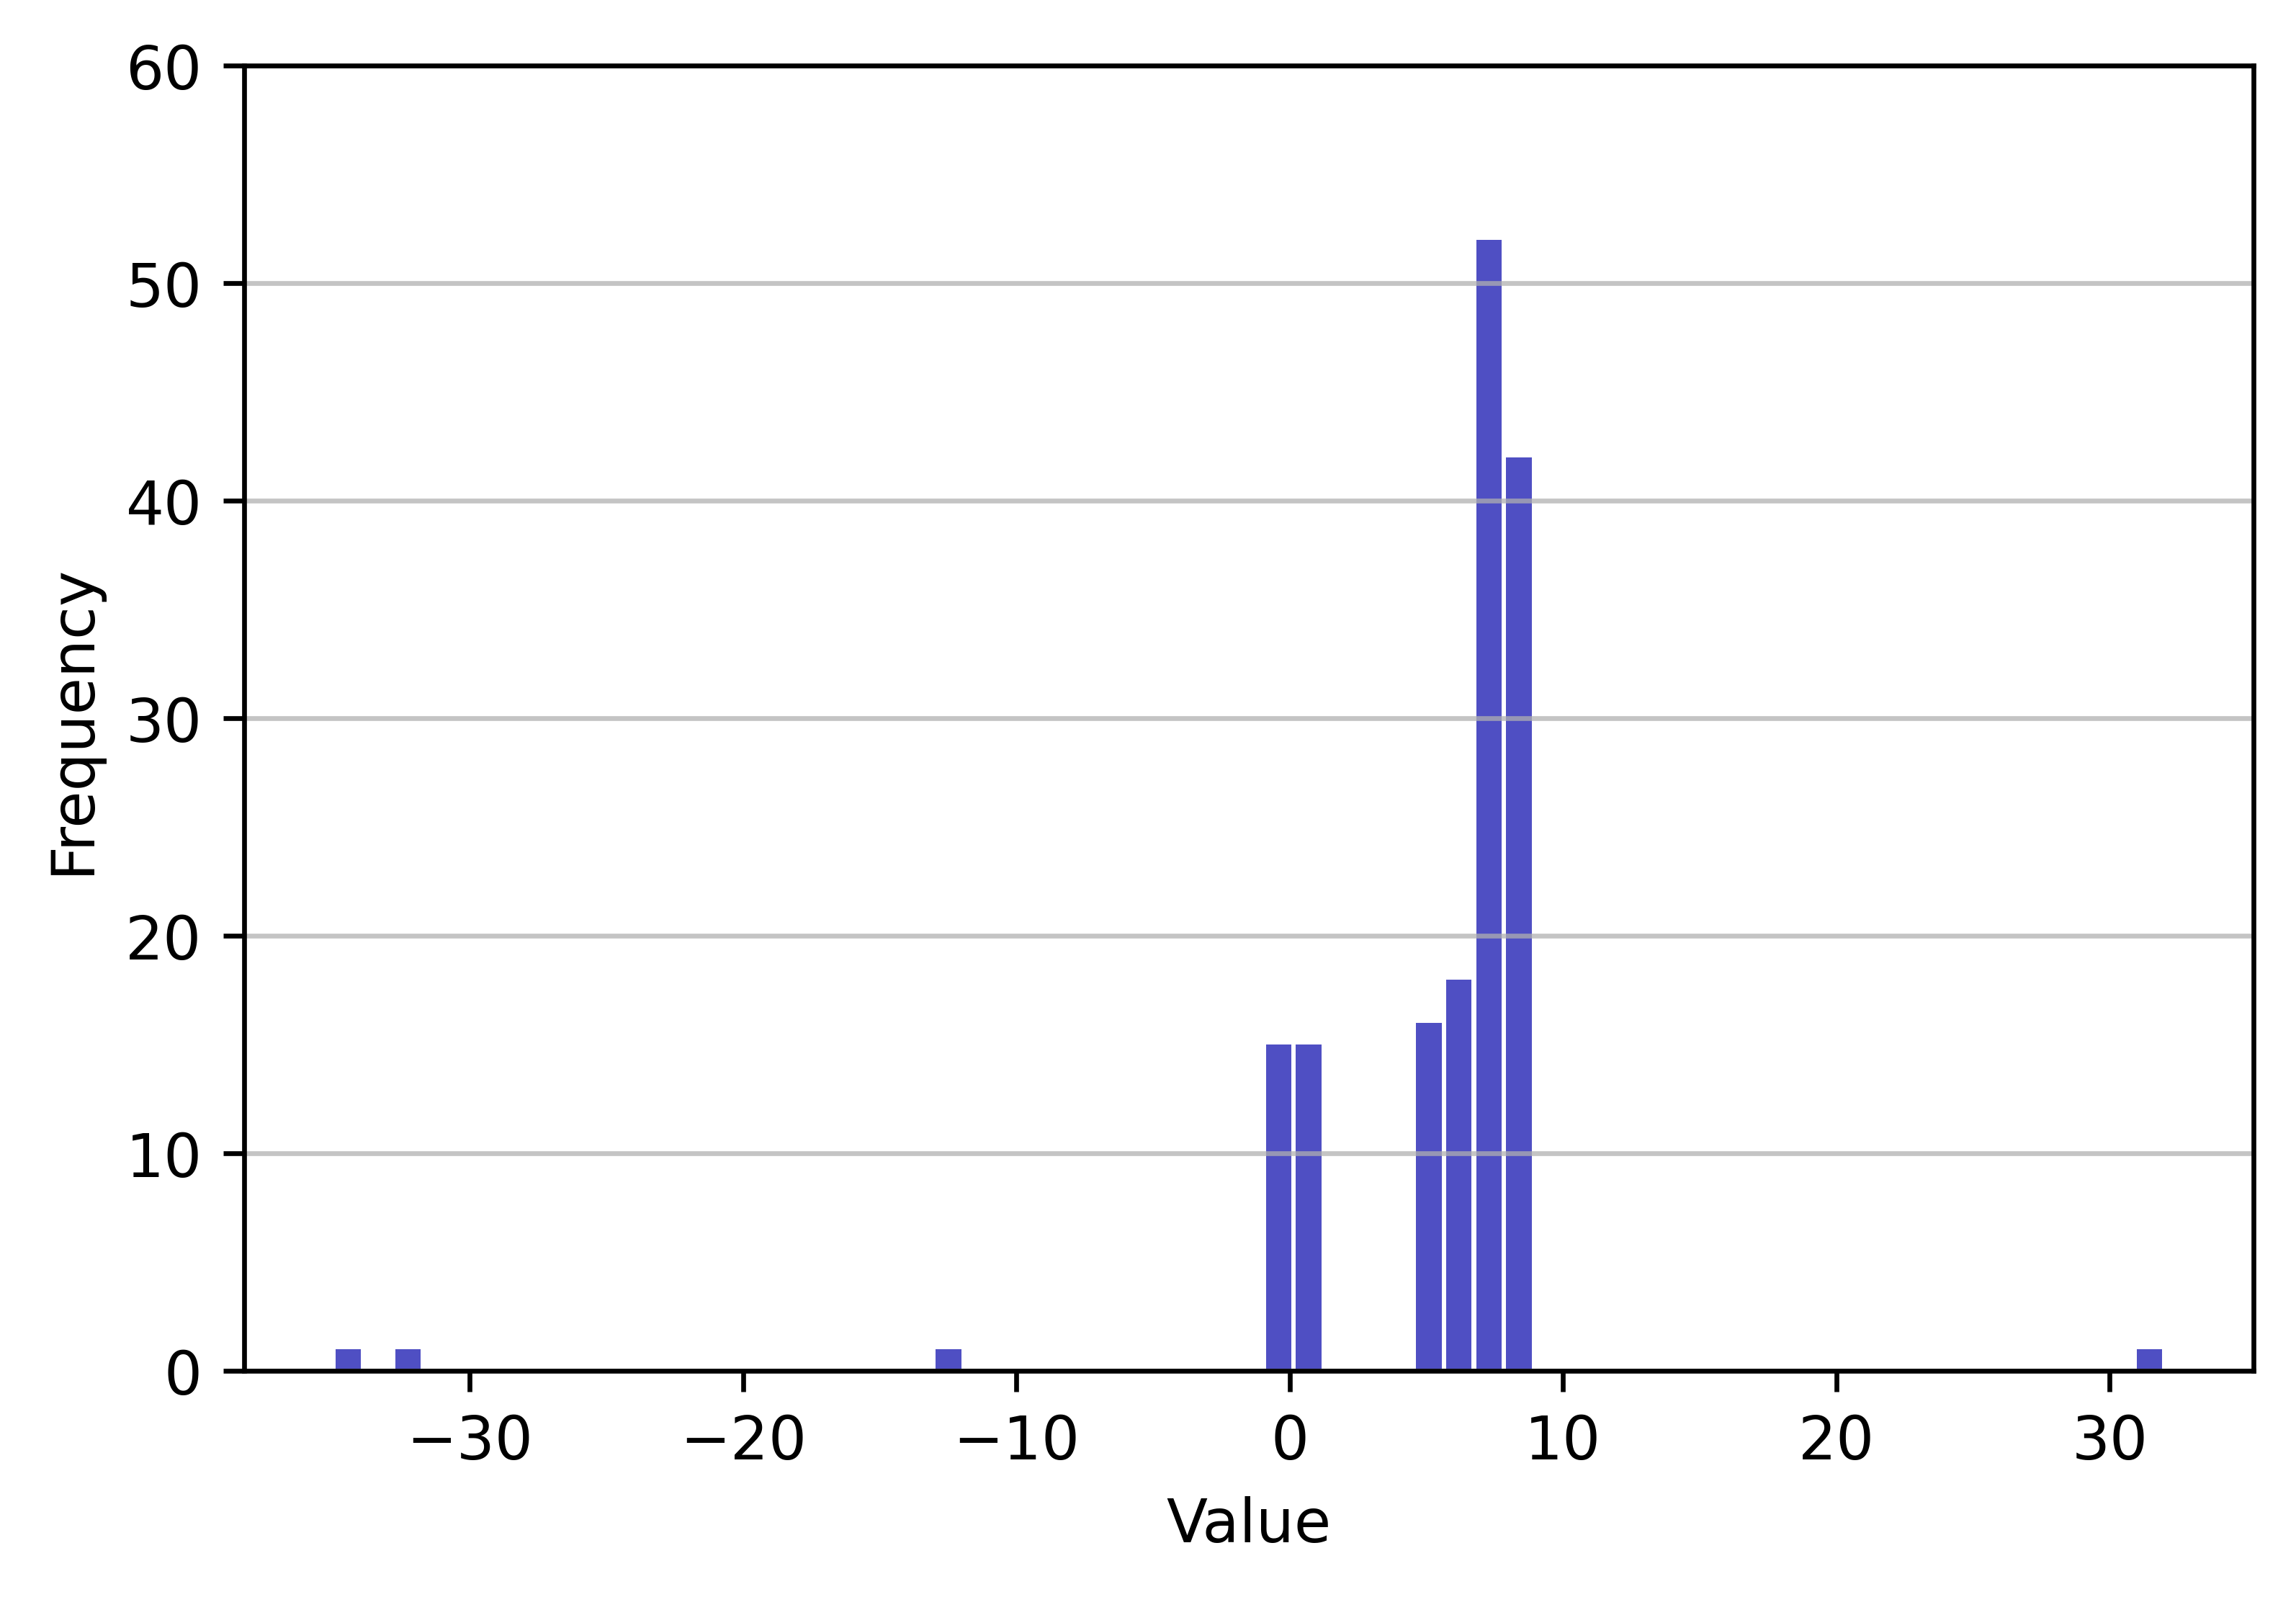
\includegraphics[scale=0.5]{Graphics/histogram-pos-all-patterns.png}}
	\subfigure[Patrón con 19 muestras]{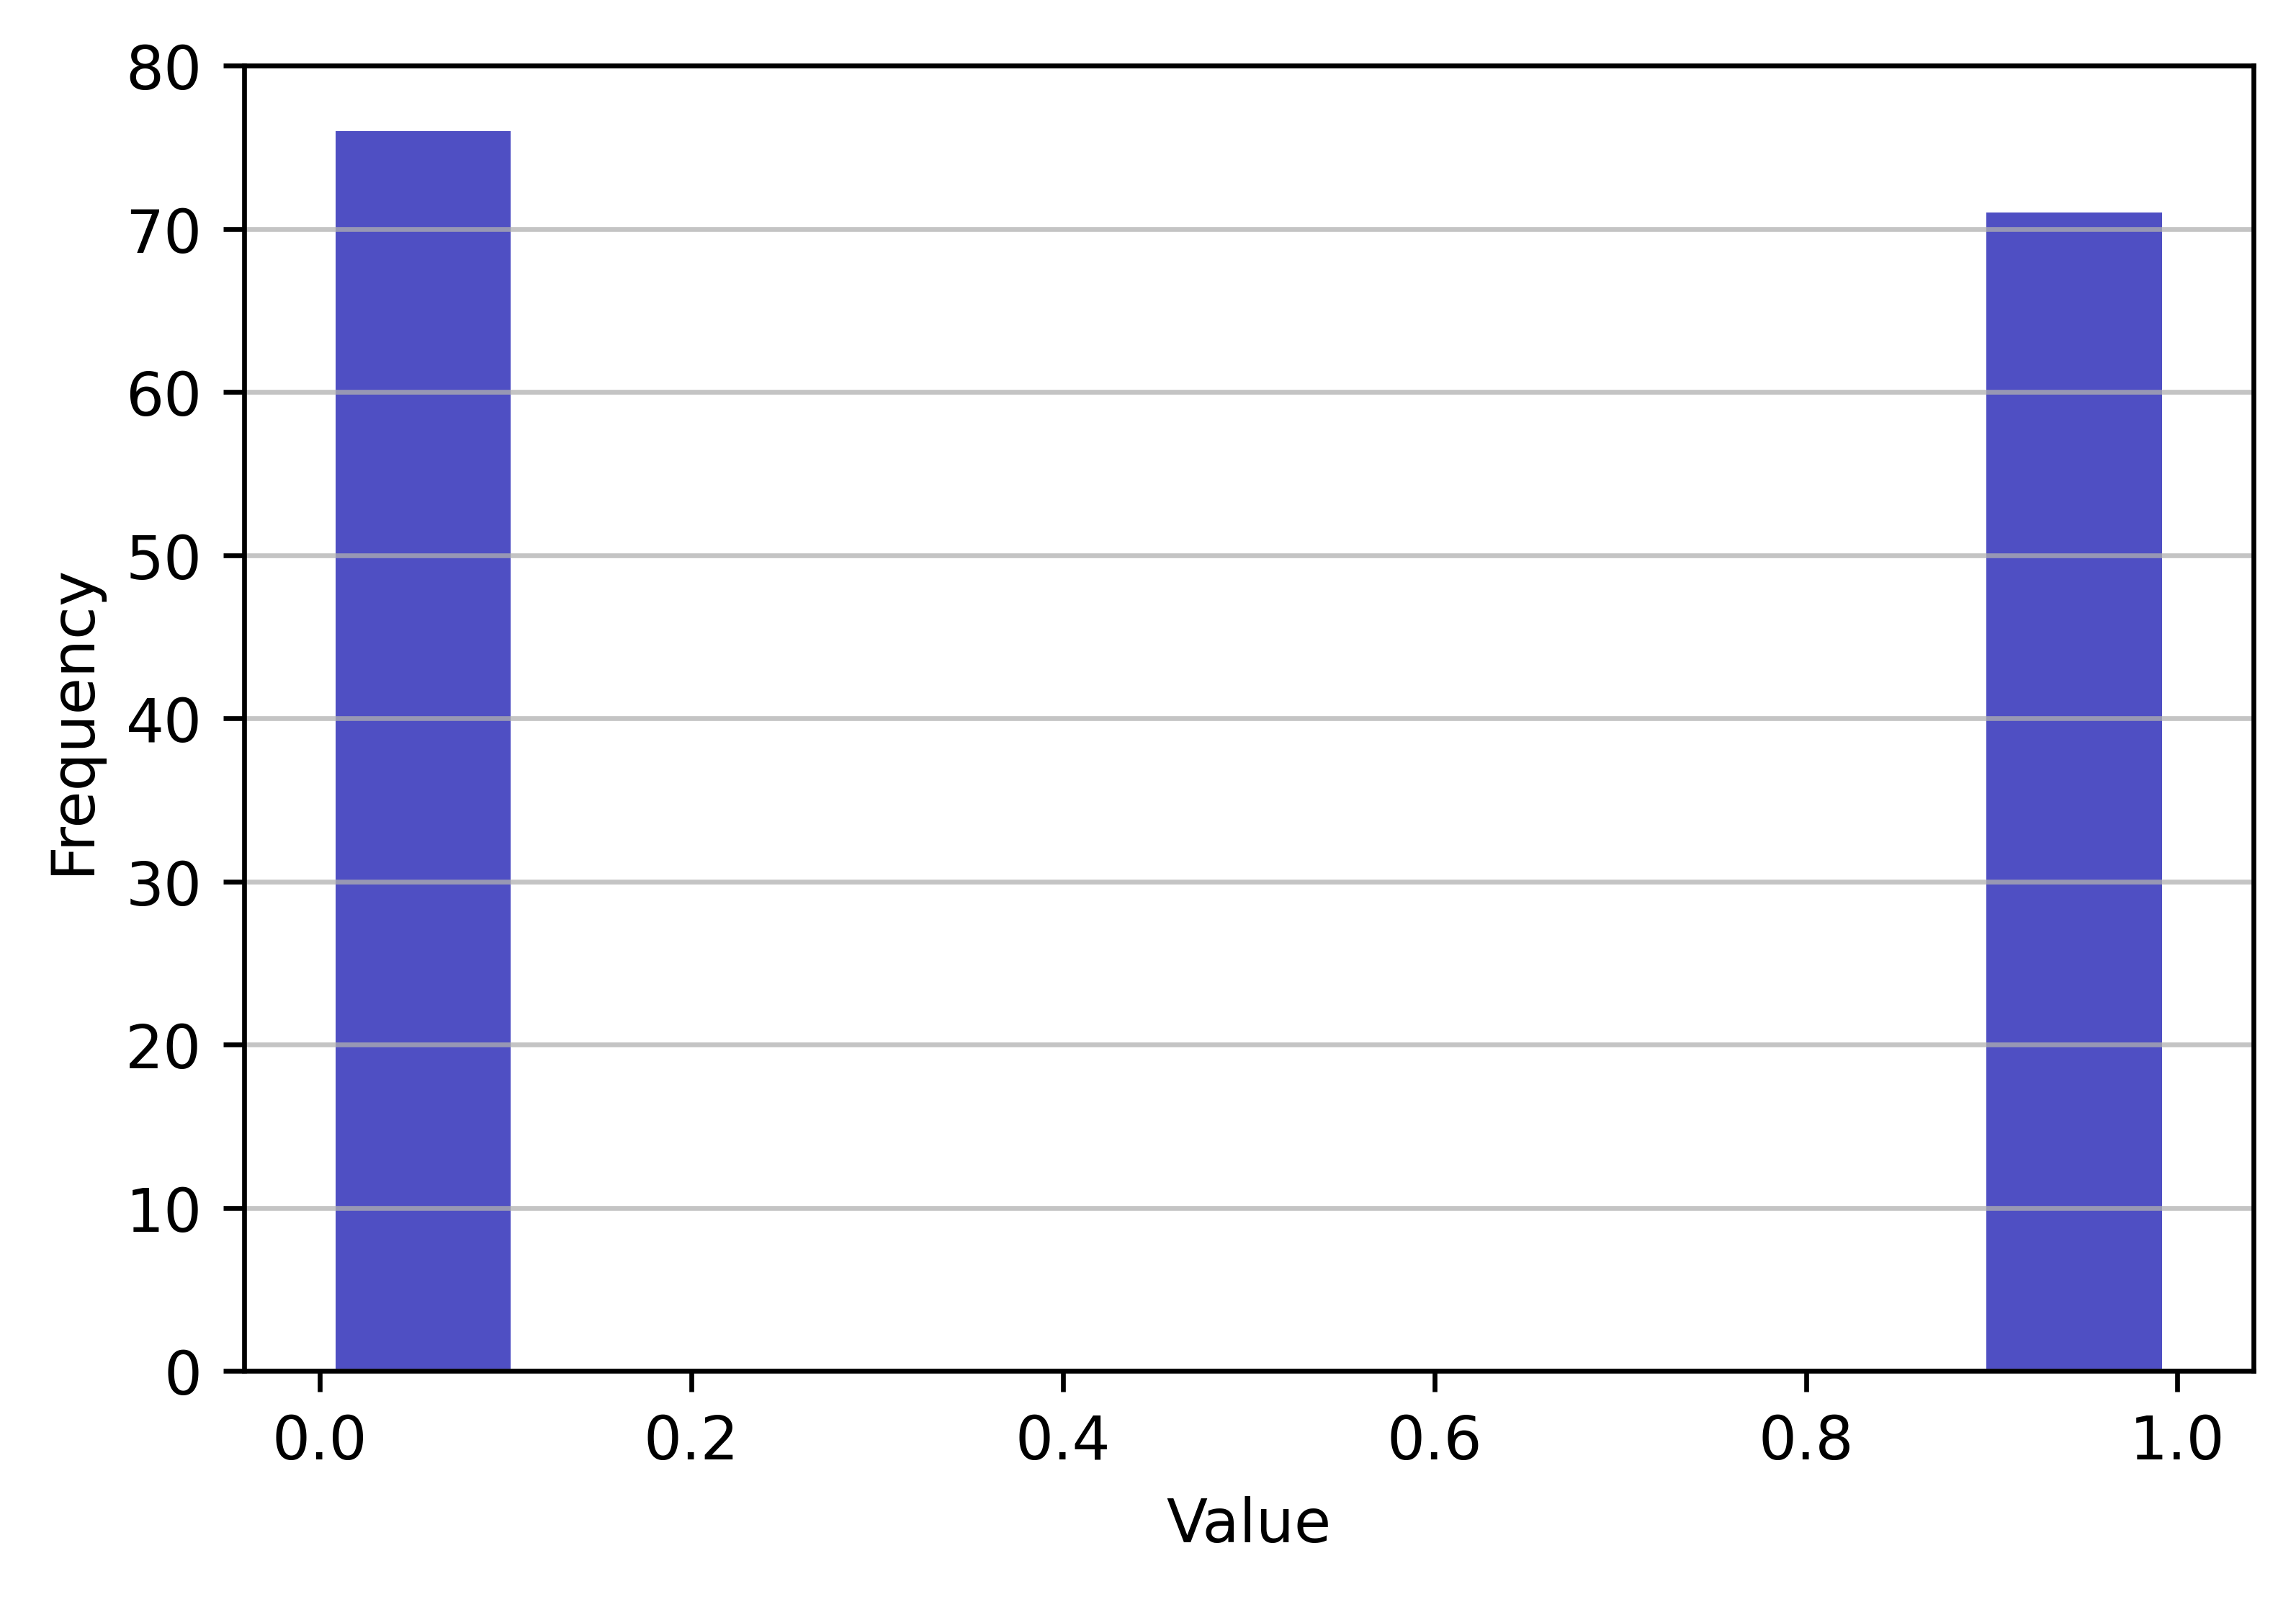
\includegraphics[scale=0.5]{Graphics/histogram-pos-long-pattern.png}}
	\subfigure[Patrón con 27 muestras]{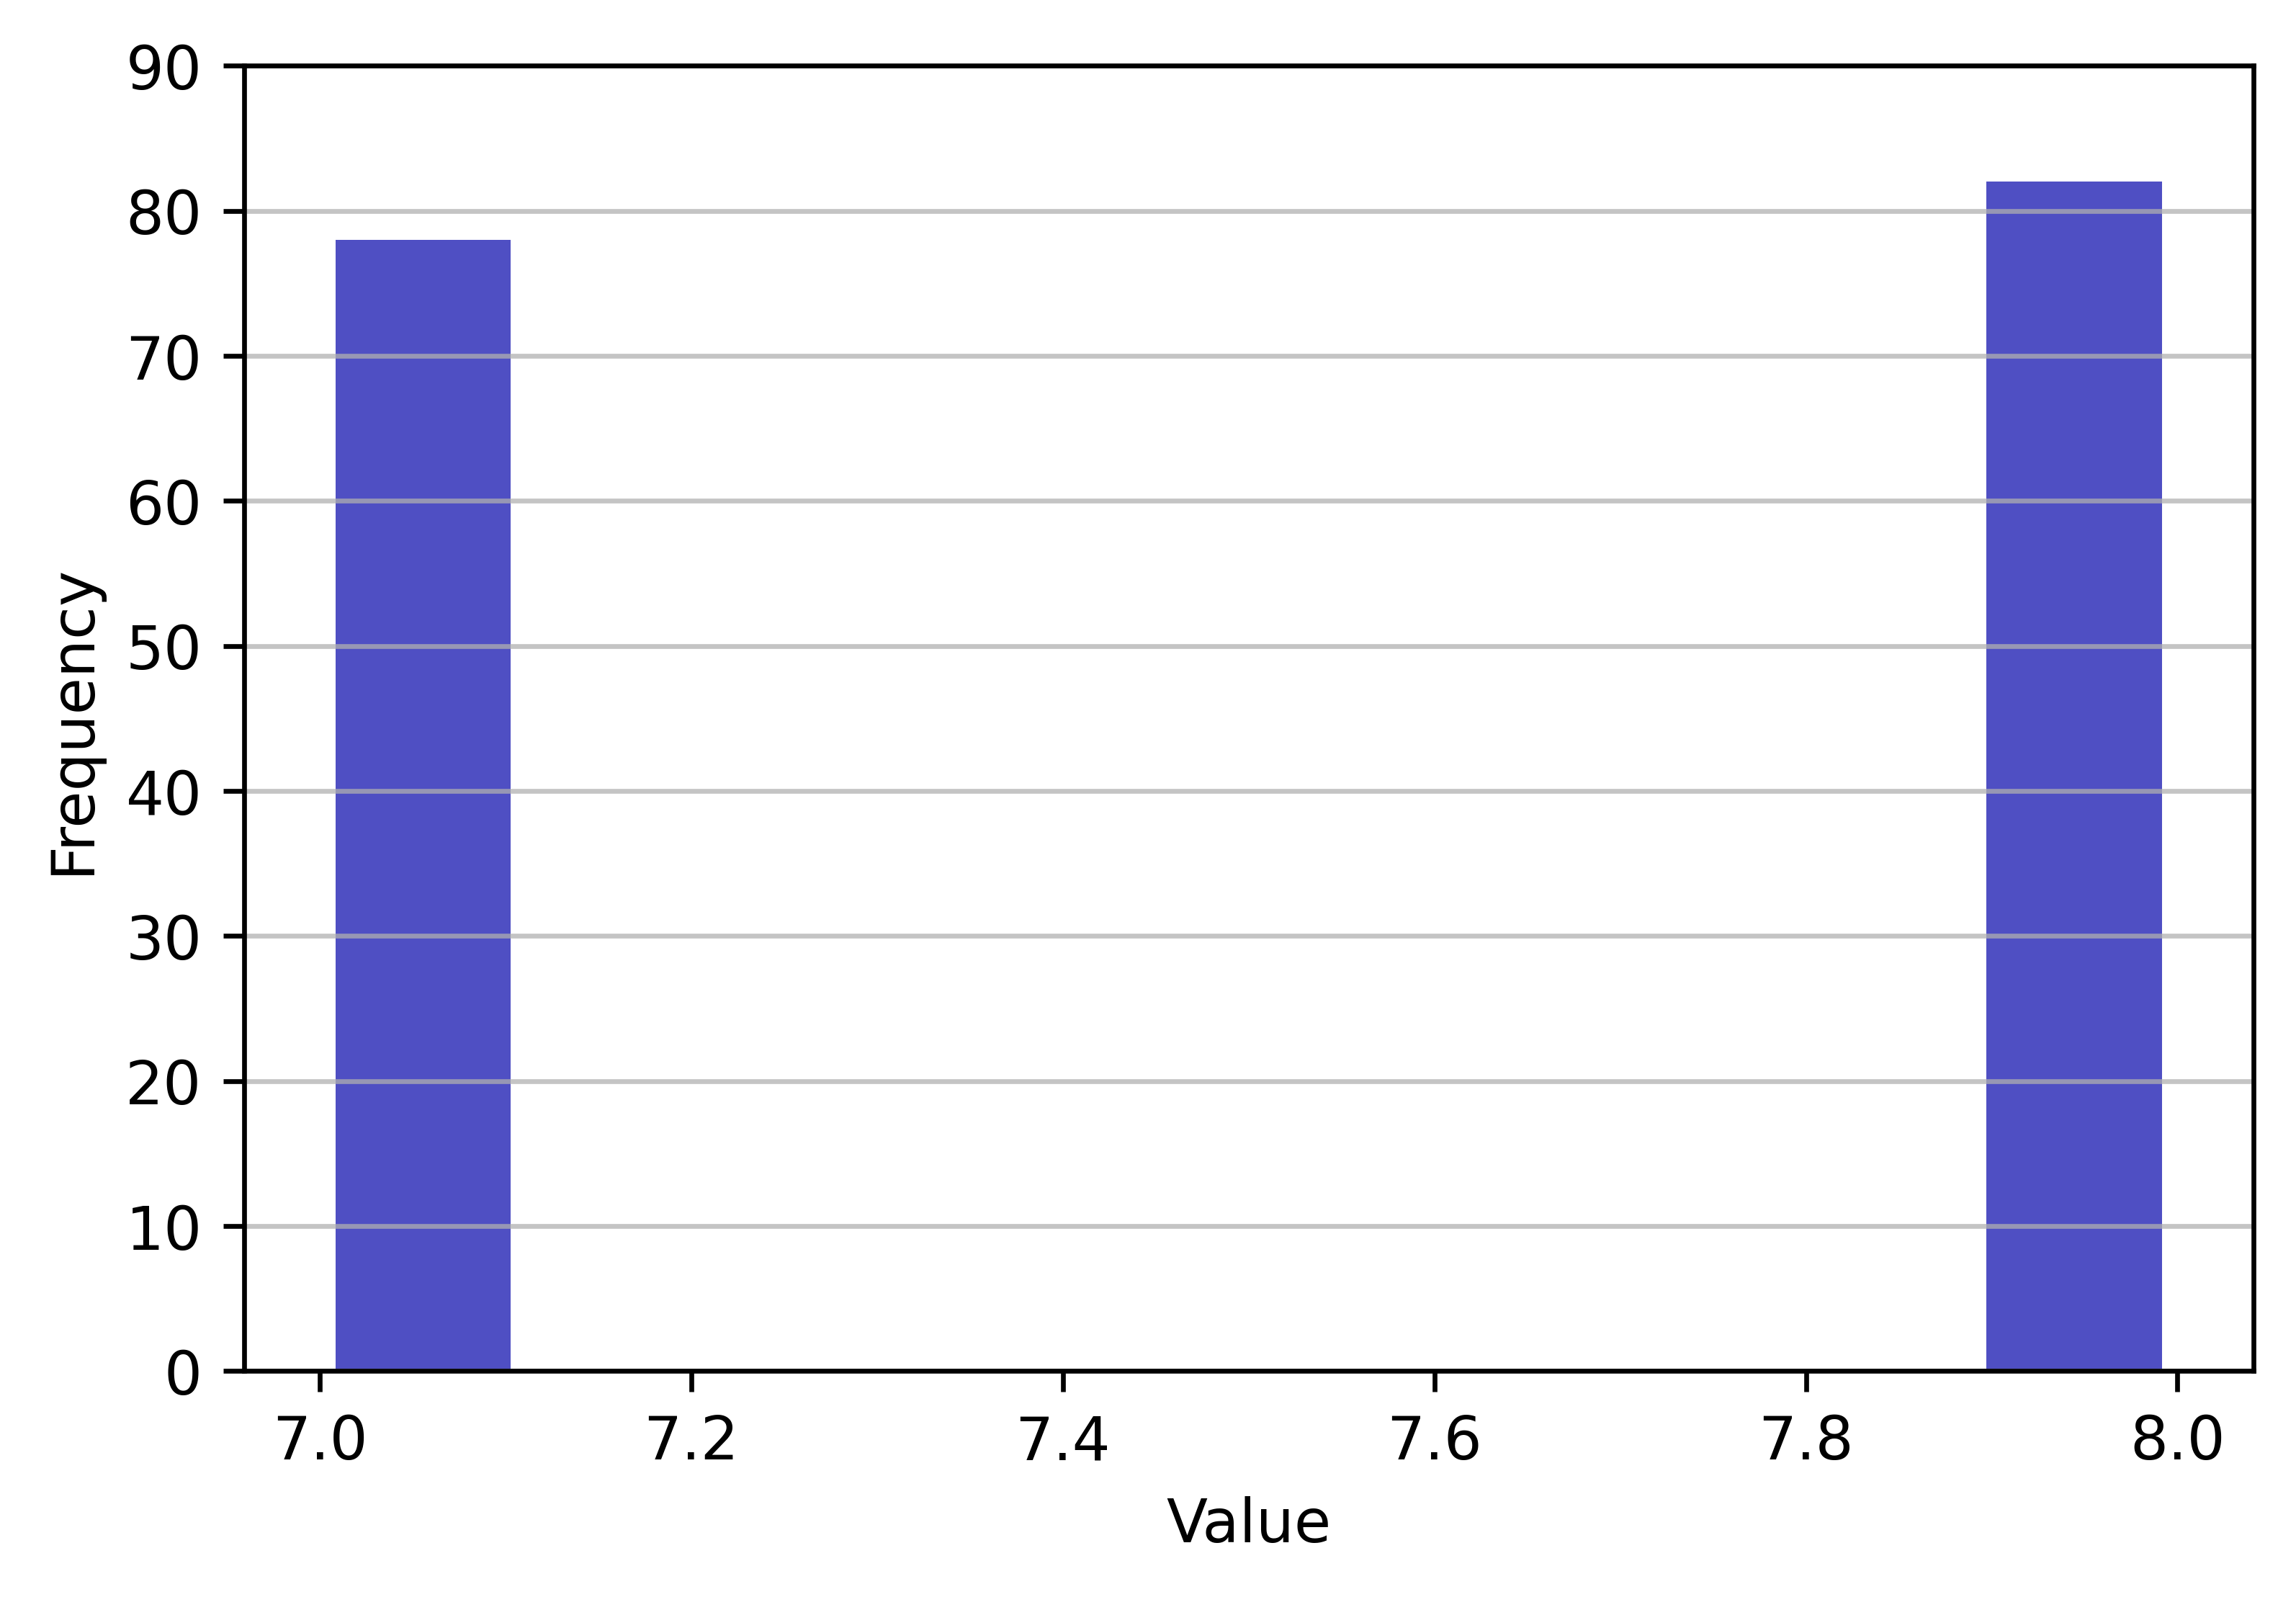
\includegraphics[scale=0.5]{Graphics/histogram-pos-medium-pattern.png}}
	\caption{ Histogramas con las frecuencias de los valores de las diferencias entre la posición real del patrón y la que predice el algoritmo.} \label{fig:hist-comparison}
\end{figure} 

\begin{figure}
	\centering
	\subfigure[Matriz de confusión]{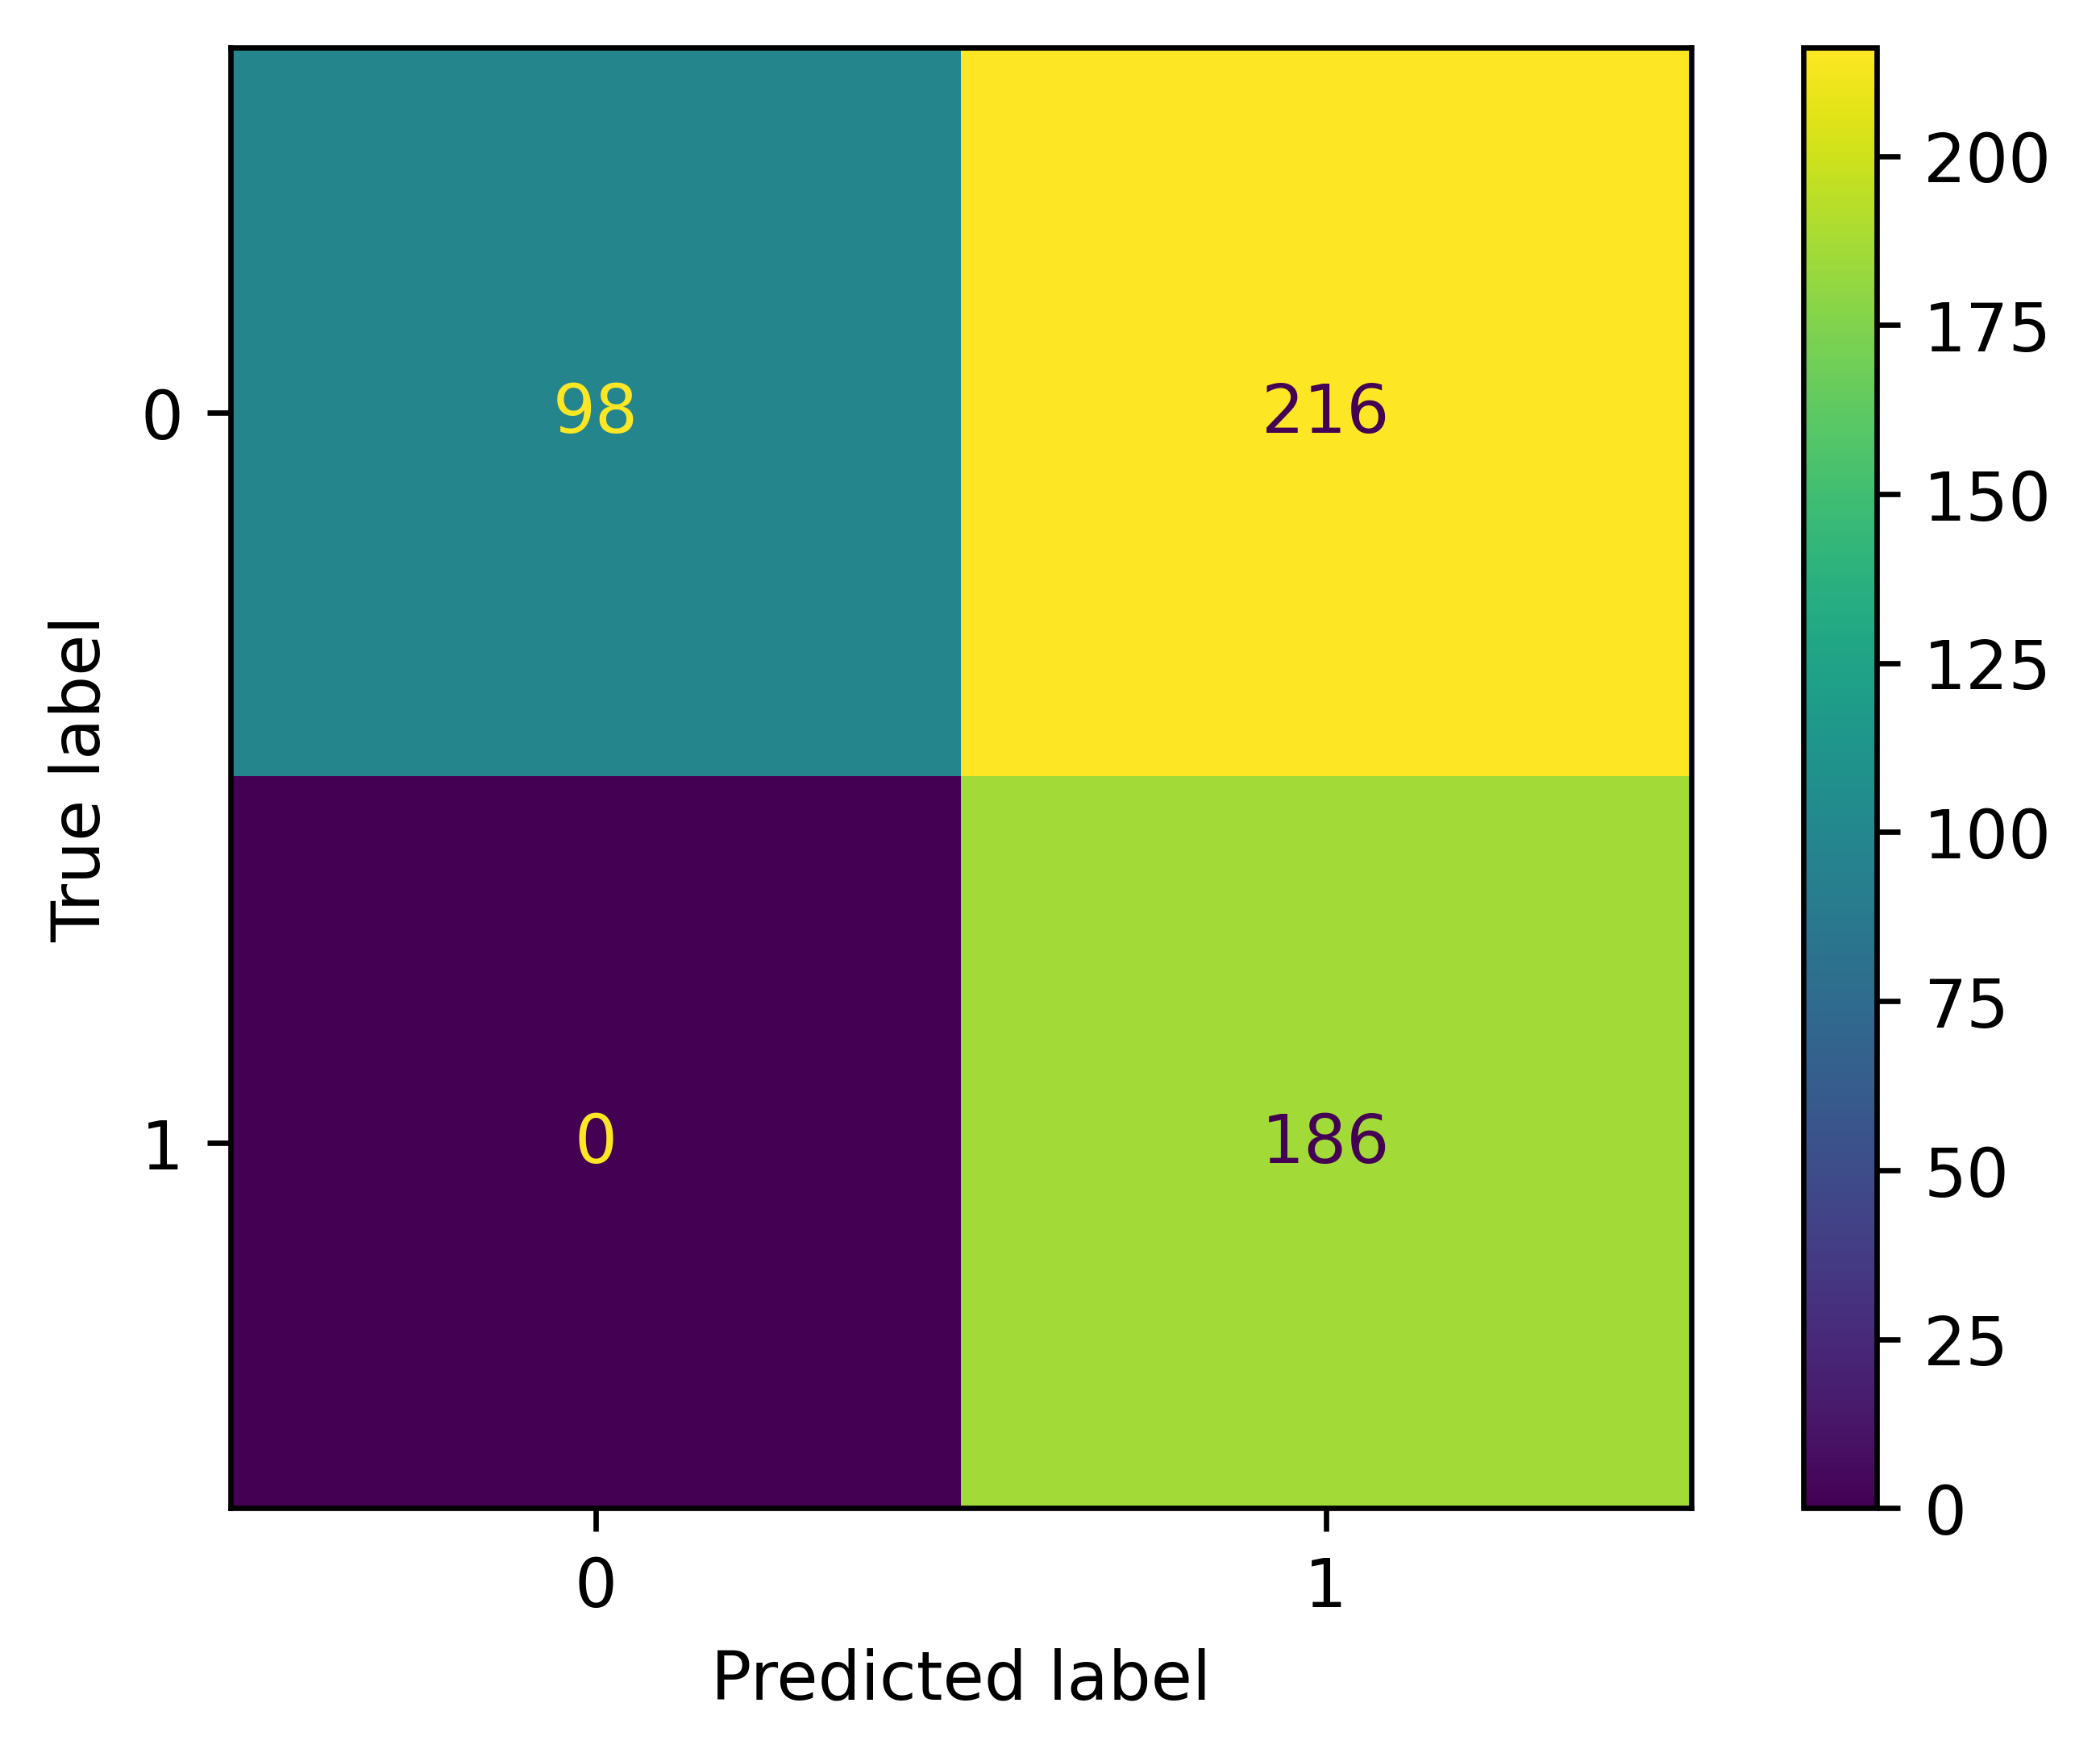
\includegraphics[scale=0.5]{Graphics/cm-th-06.png}}
	\subfigure[Curva ROC]{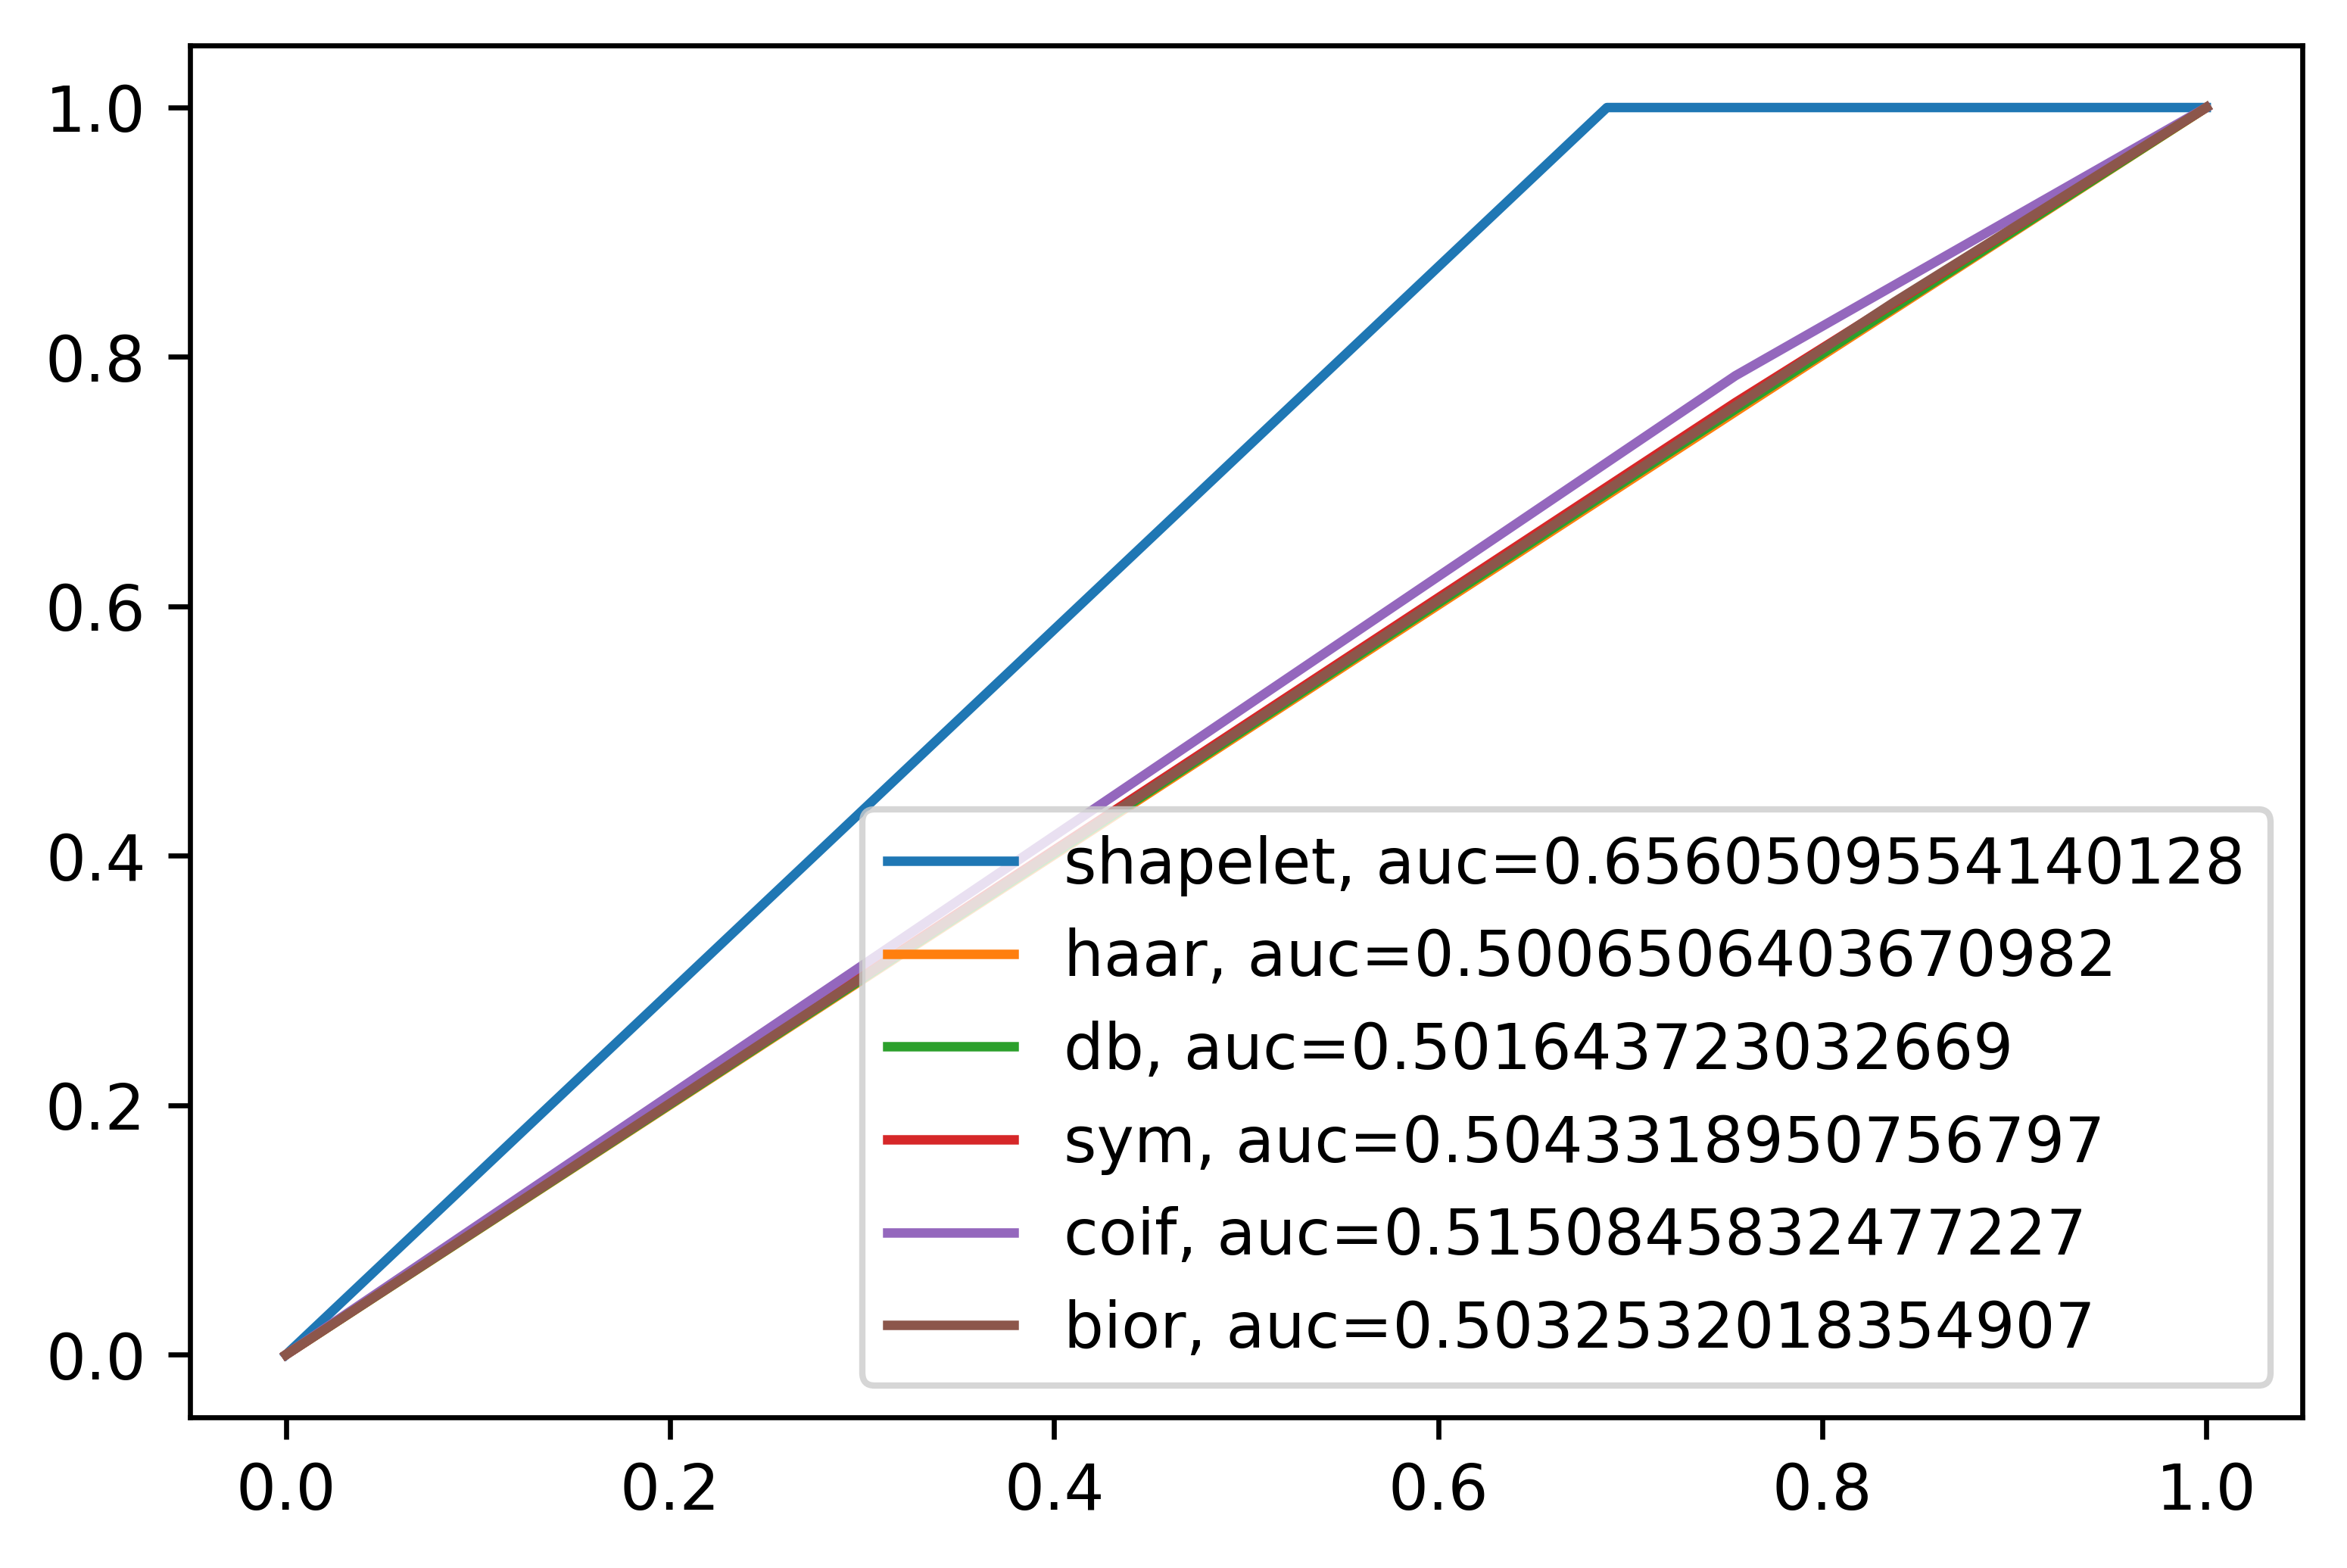
\includegraphics[scale=0.5]{Graphics/roc-th-06.png}}
	\caption{Matriz de confusión y curva ROC. En este ejemplo se tomó como umbral $th=0.60$ y un patrón de longitud 17.} \label{fig:1d-experiment-060}
\end{figure}

\begin{figure}
	\centering
	\subfigure[Matriz de confusión]{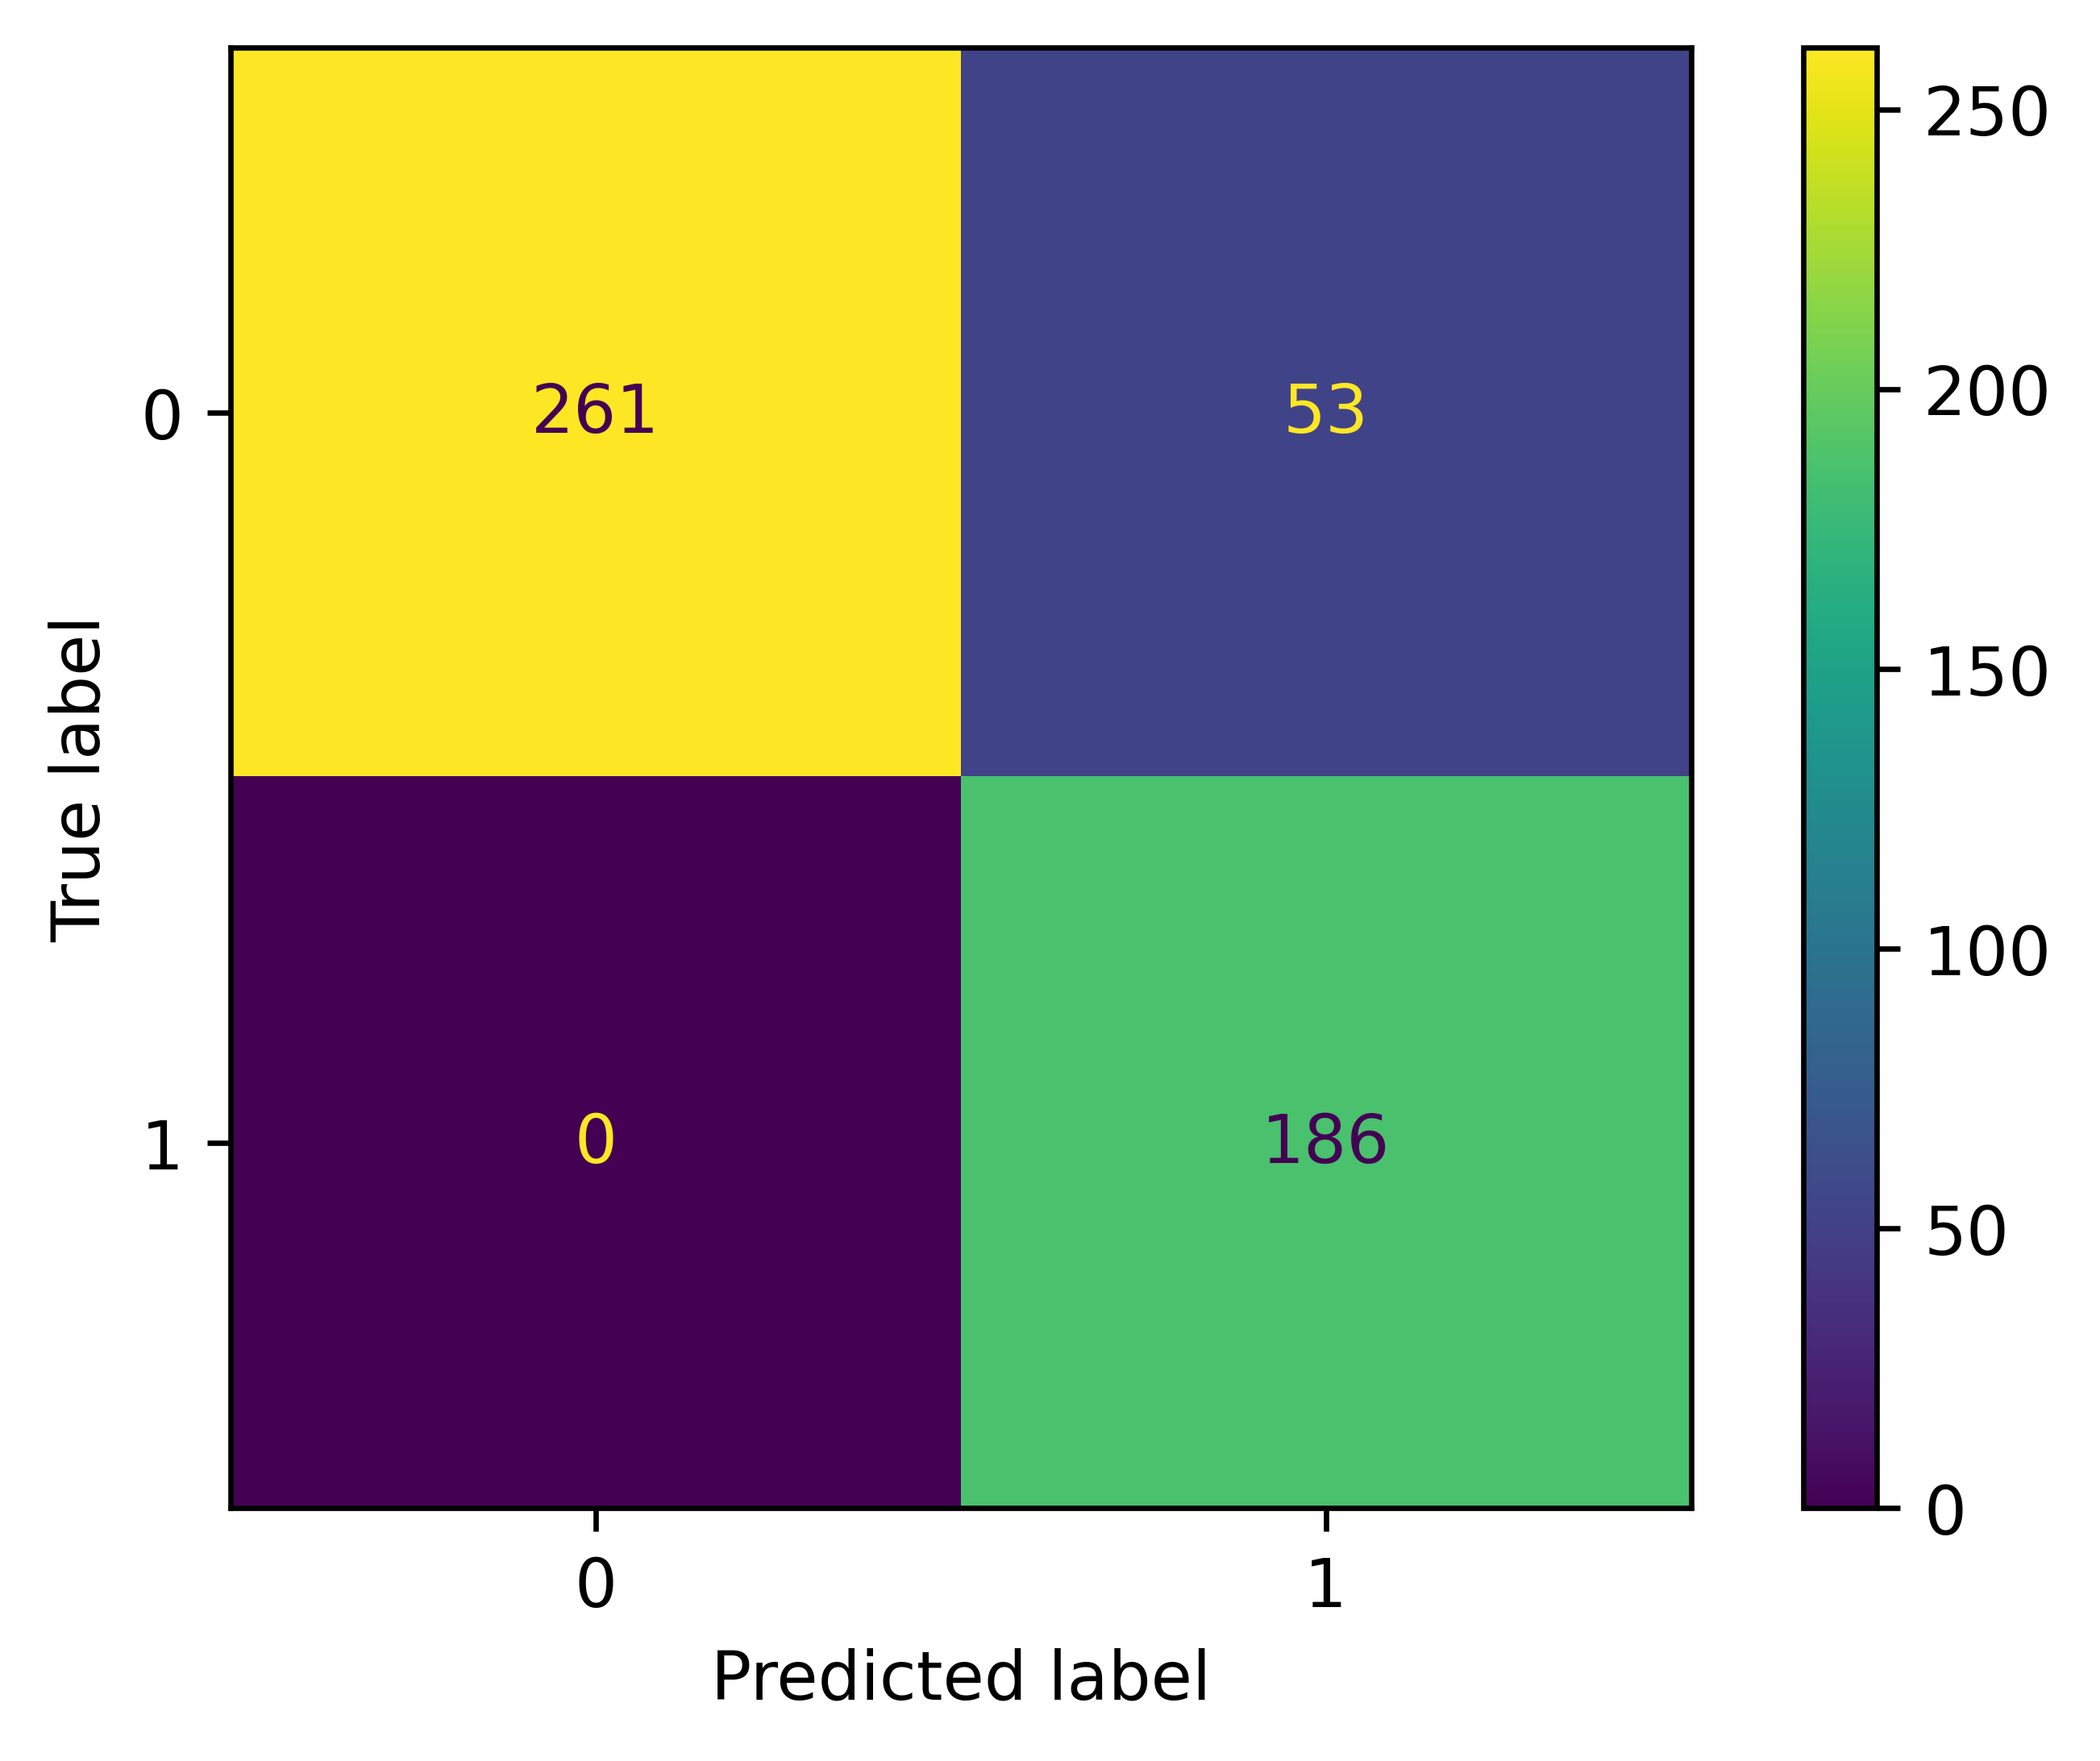
\includegraphics[scale=0.5]{Graphics/cm-th-085.png}}
	\subfigure[Curva ROC]{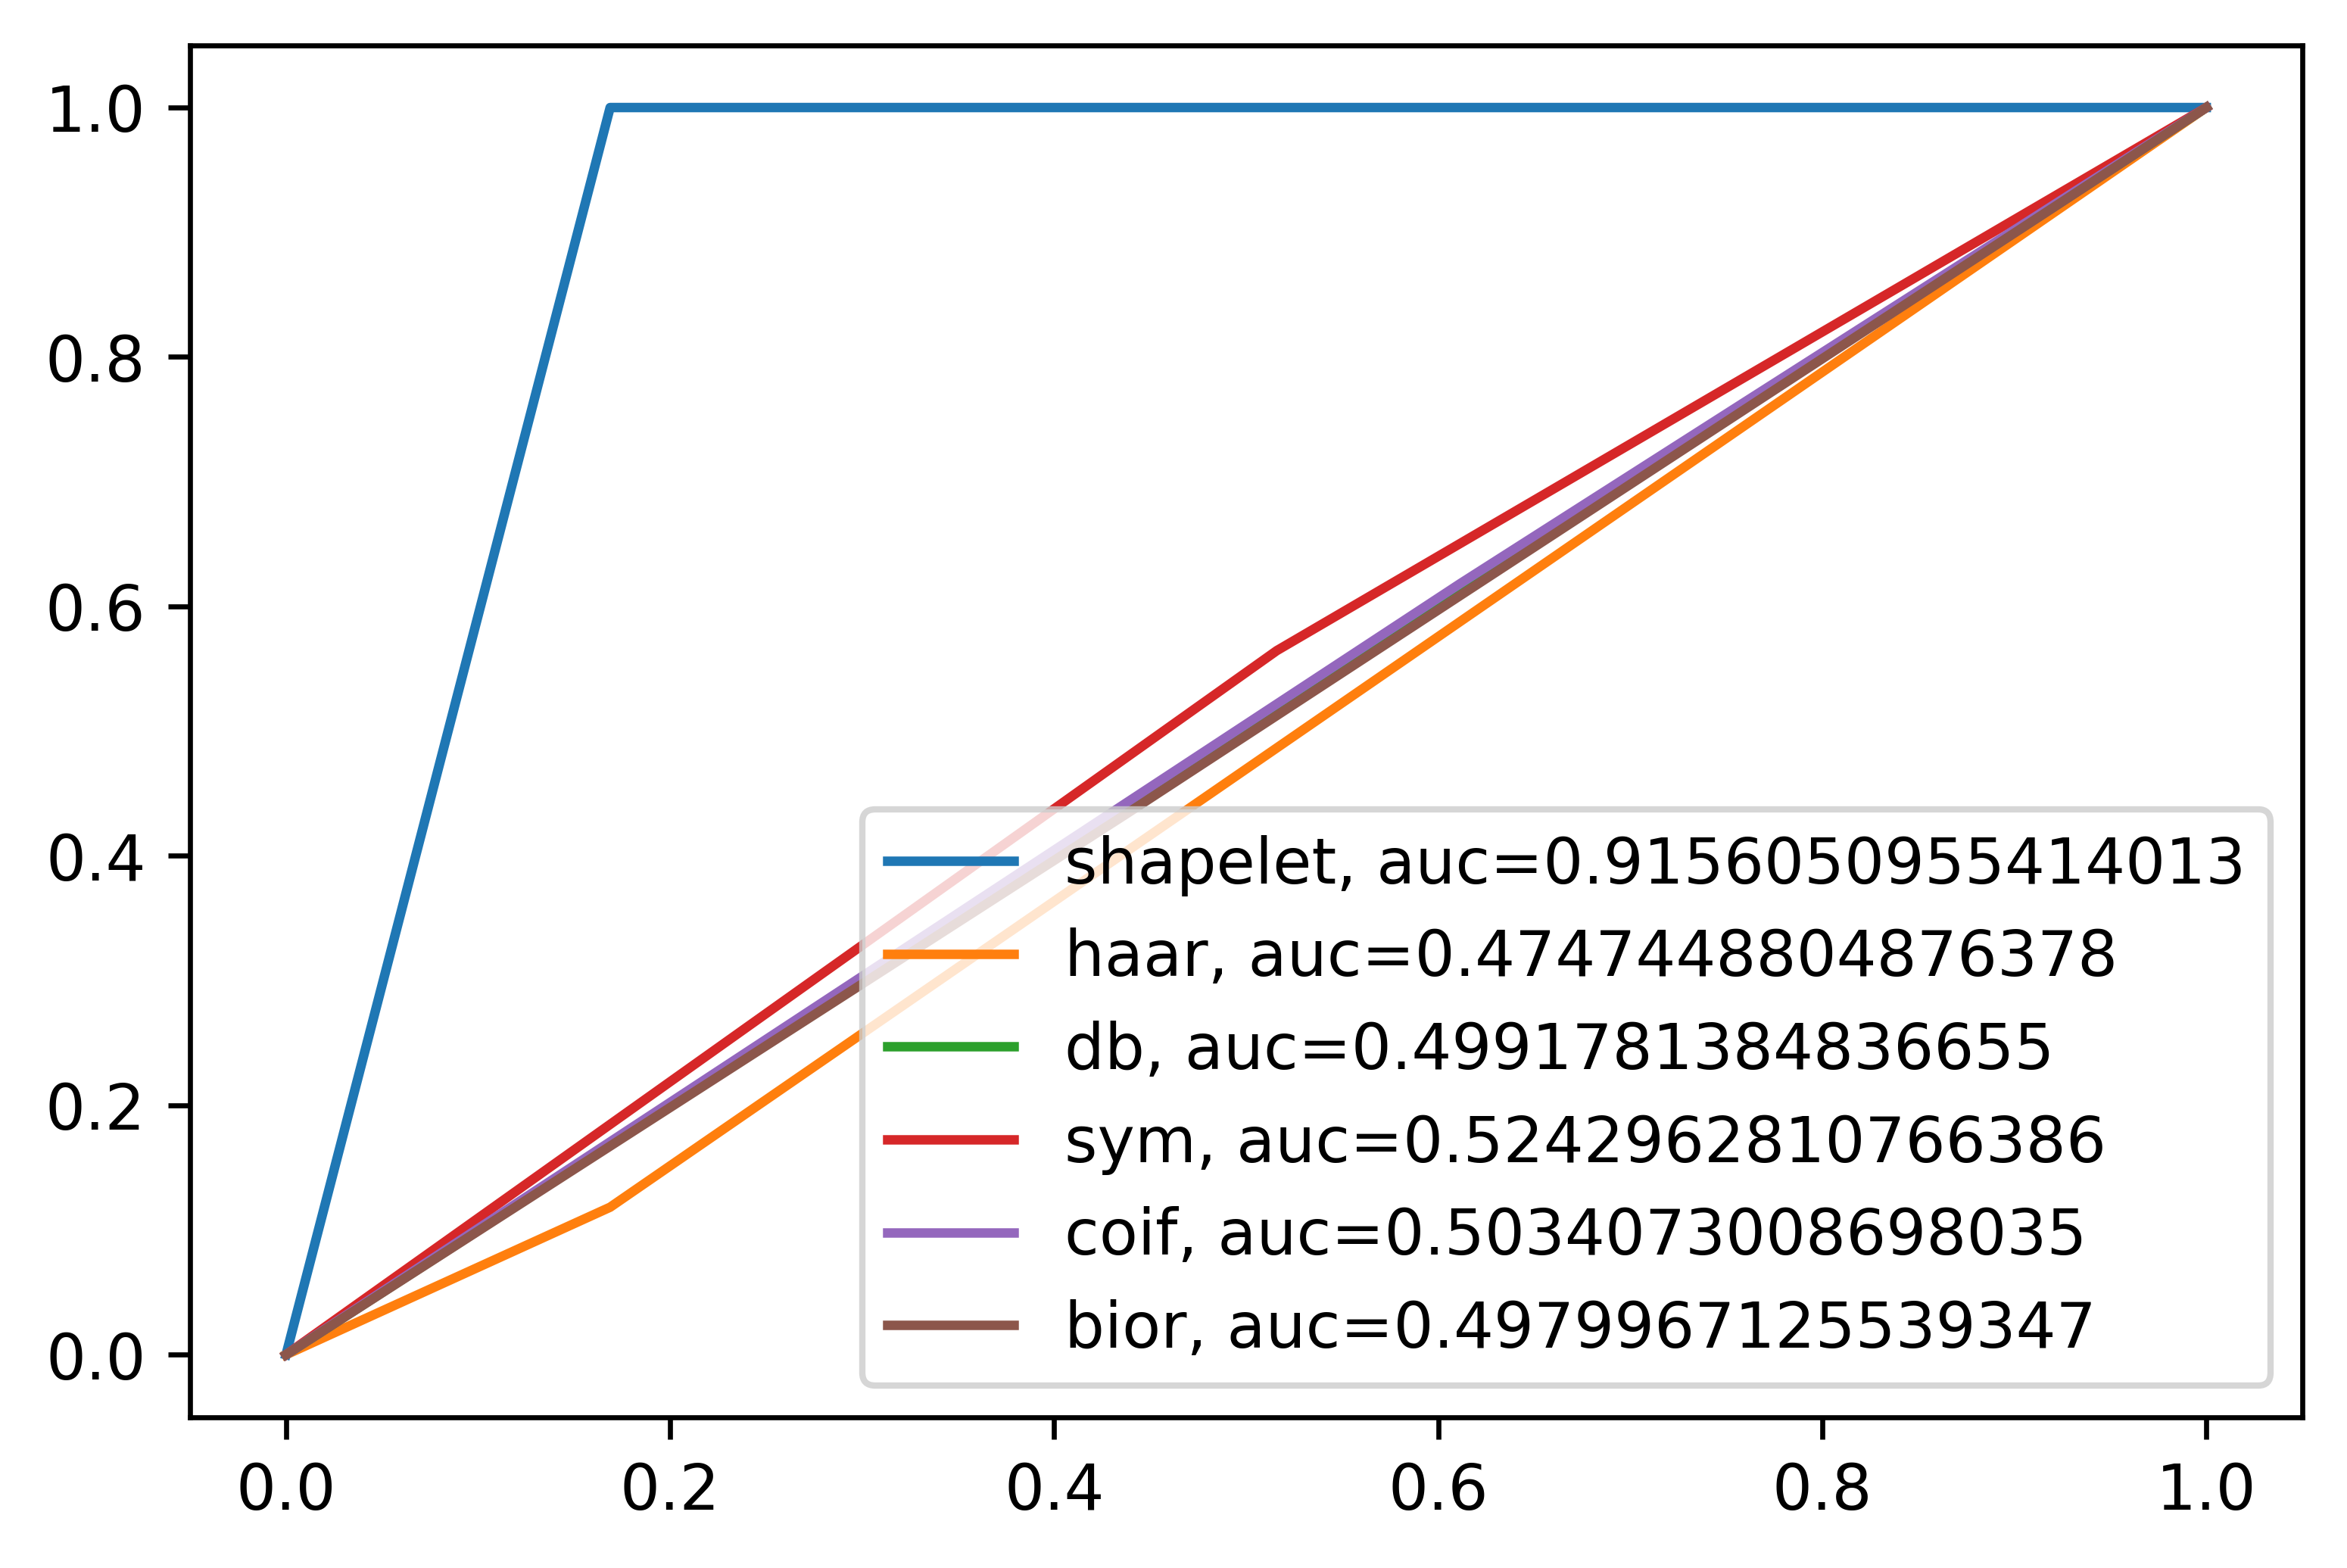
\includegraphics[scale=0.5]{Graphics/roc-th-085.png}}
	\caption{Matriz de confusión y curva ROC. En este ejemplo se tomó como umbral $th=0.85$ y un patrón de longitud 17.} \label{fig:1d-experiment-085}
\end{figure}

\begin{figure}
	\centering
	\subfigure[Matriz de confusión]{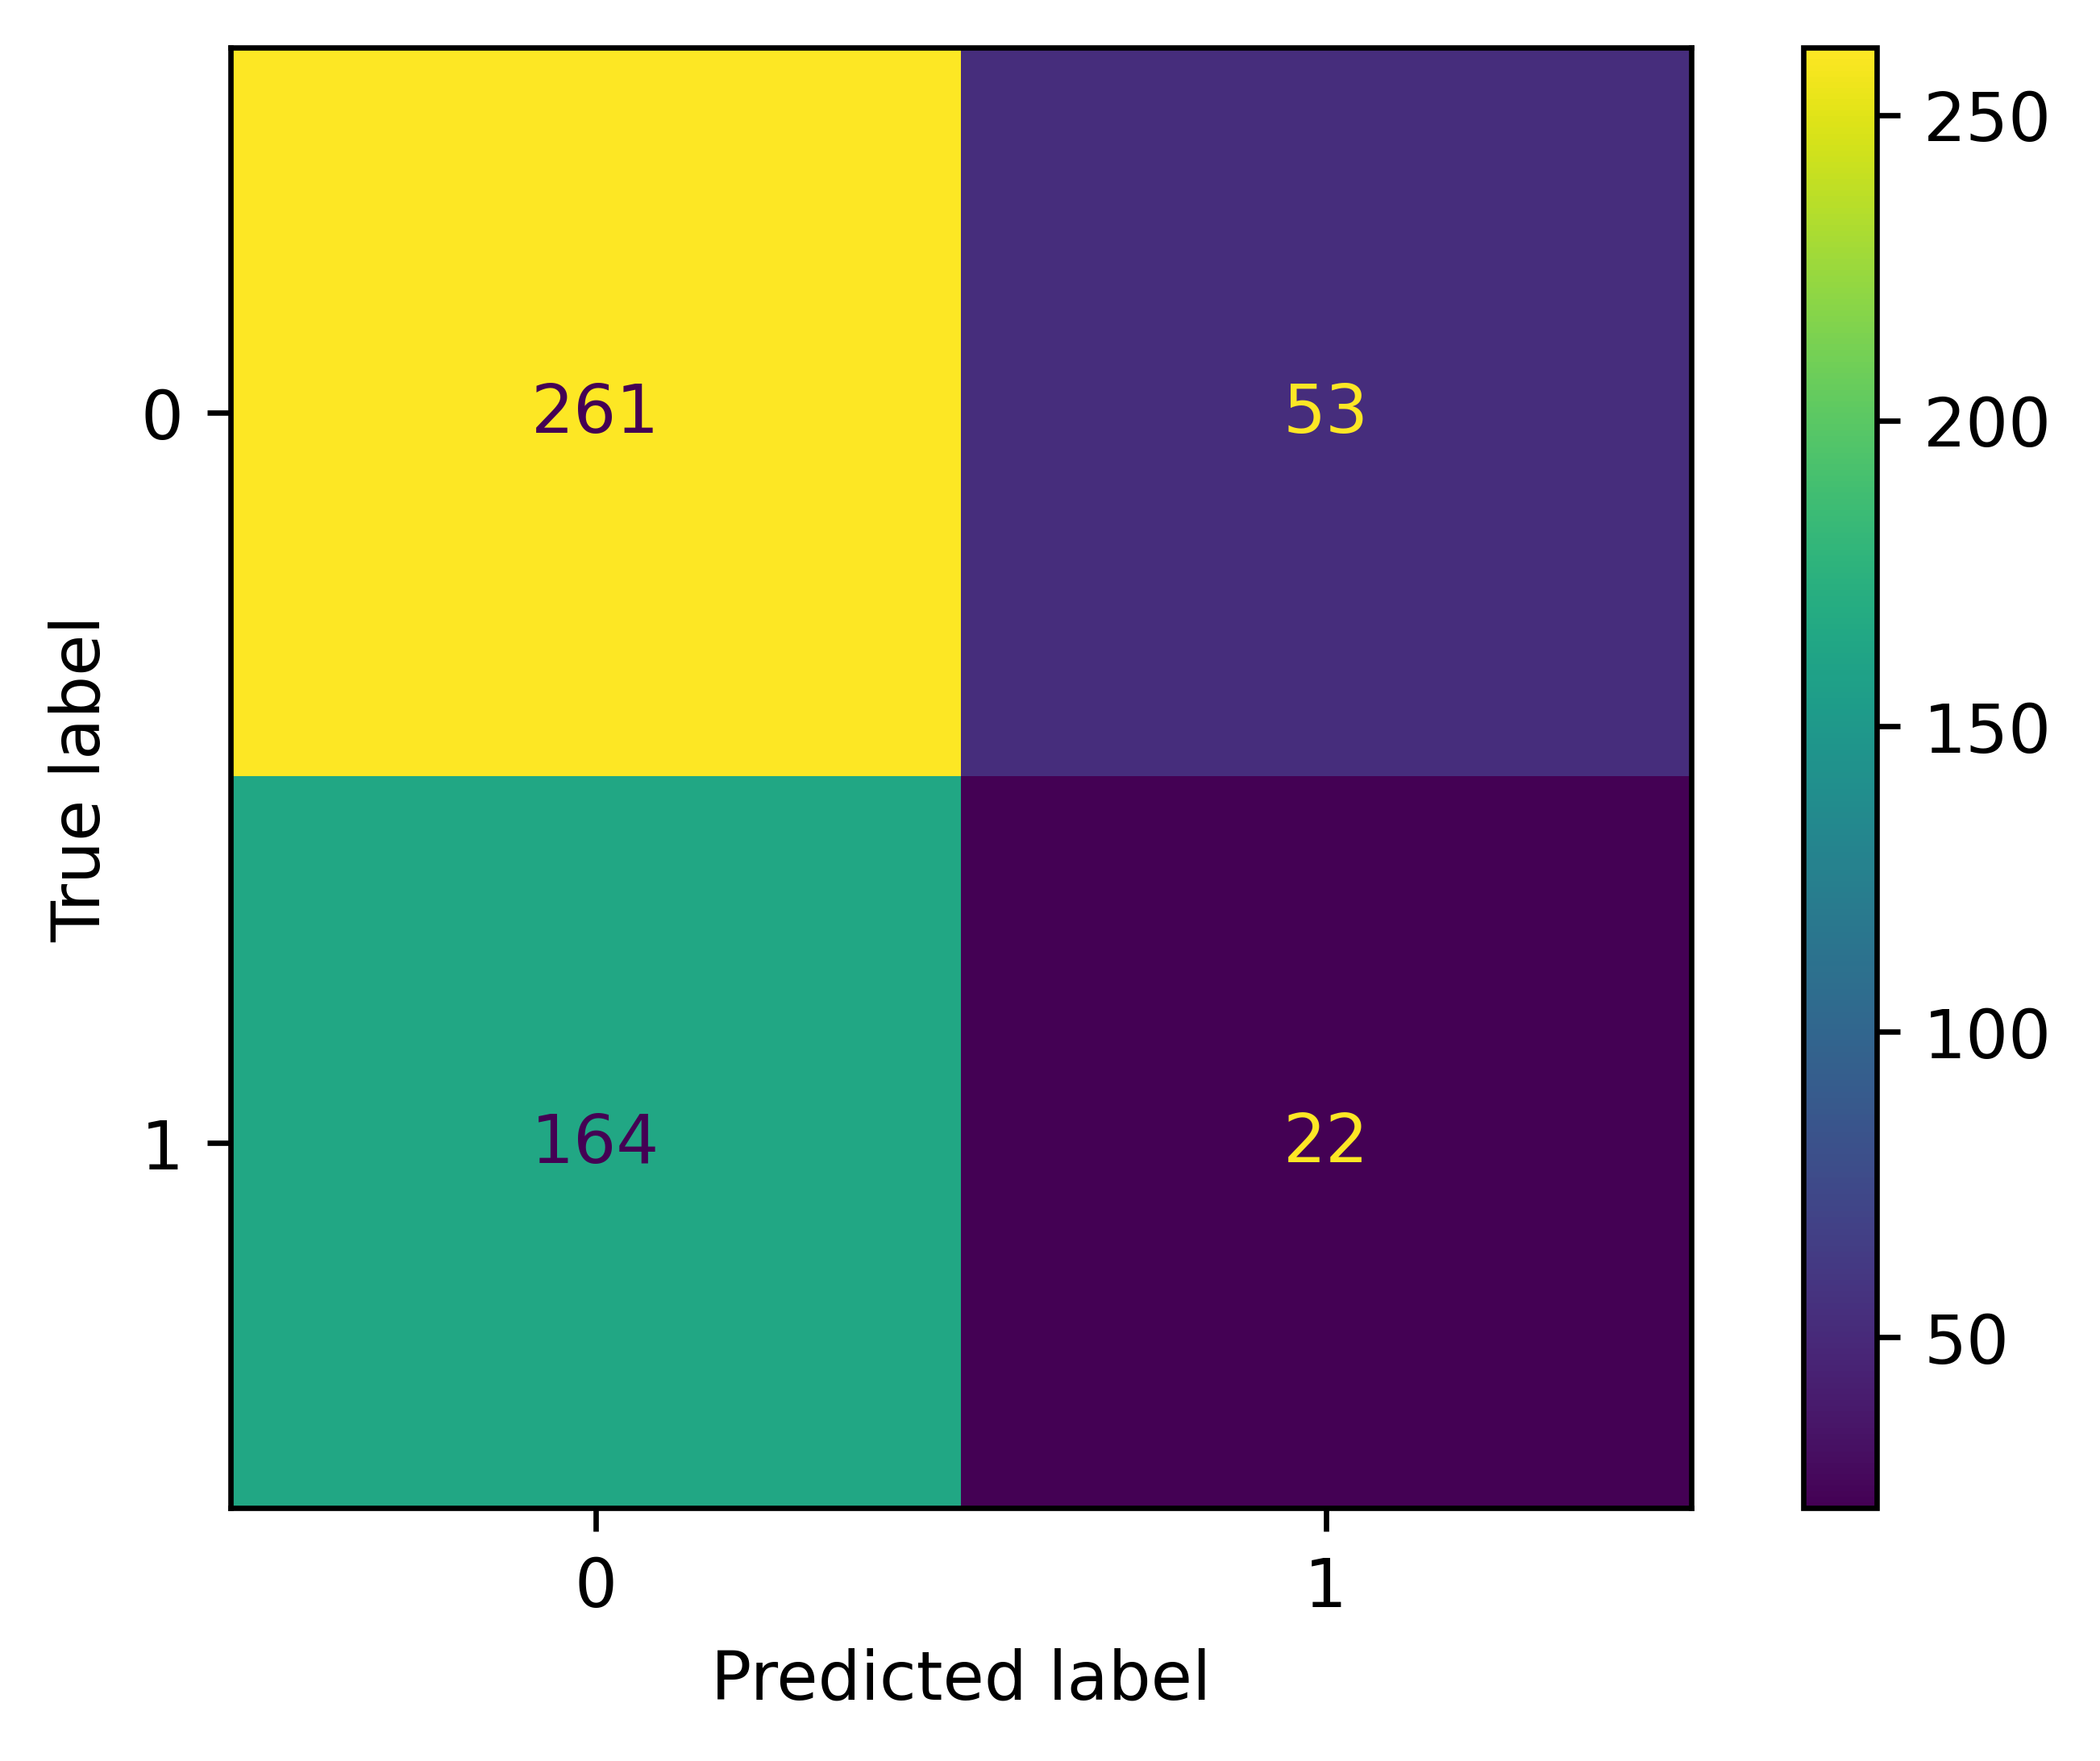
\includegraphics[scale=0.5]{Graphics/cm-th-098.png}}
	\subfigure[Curva ROC]{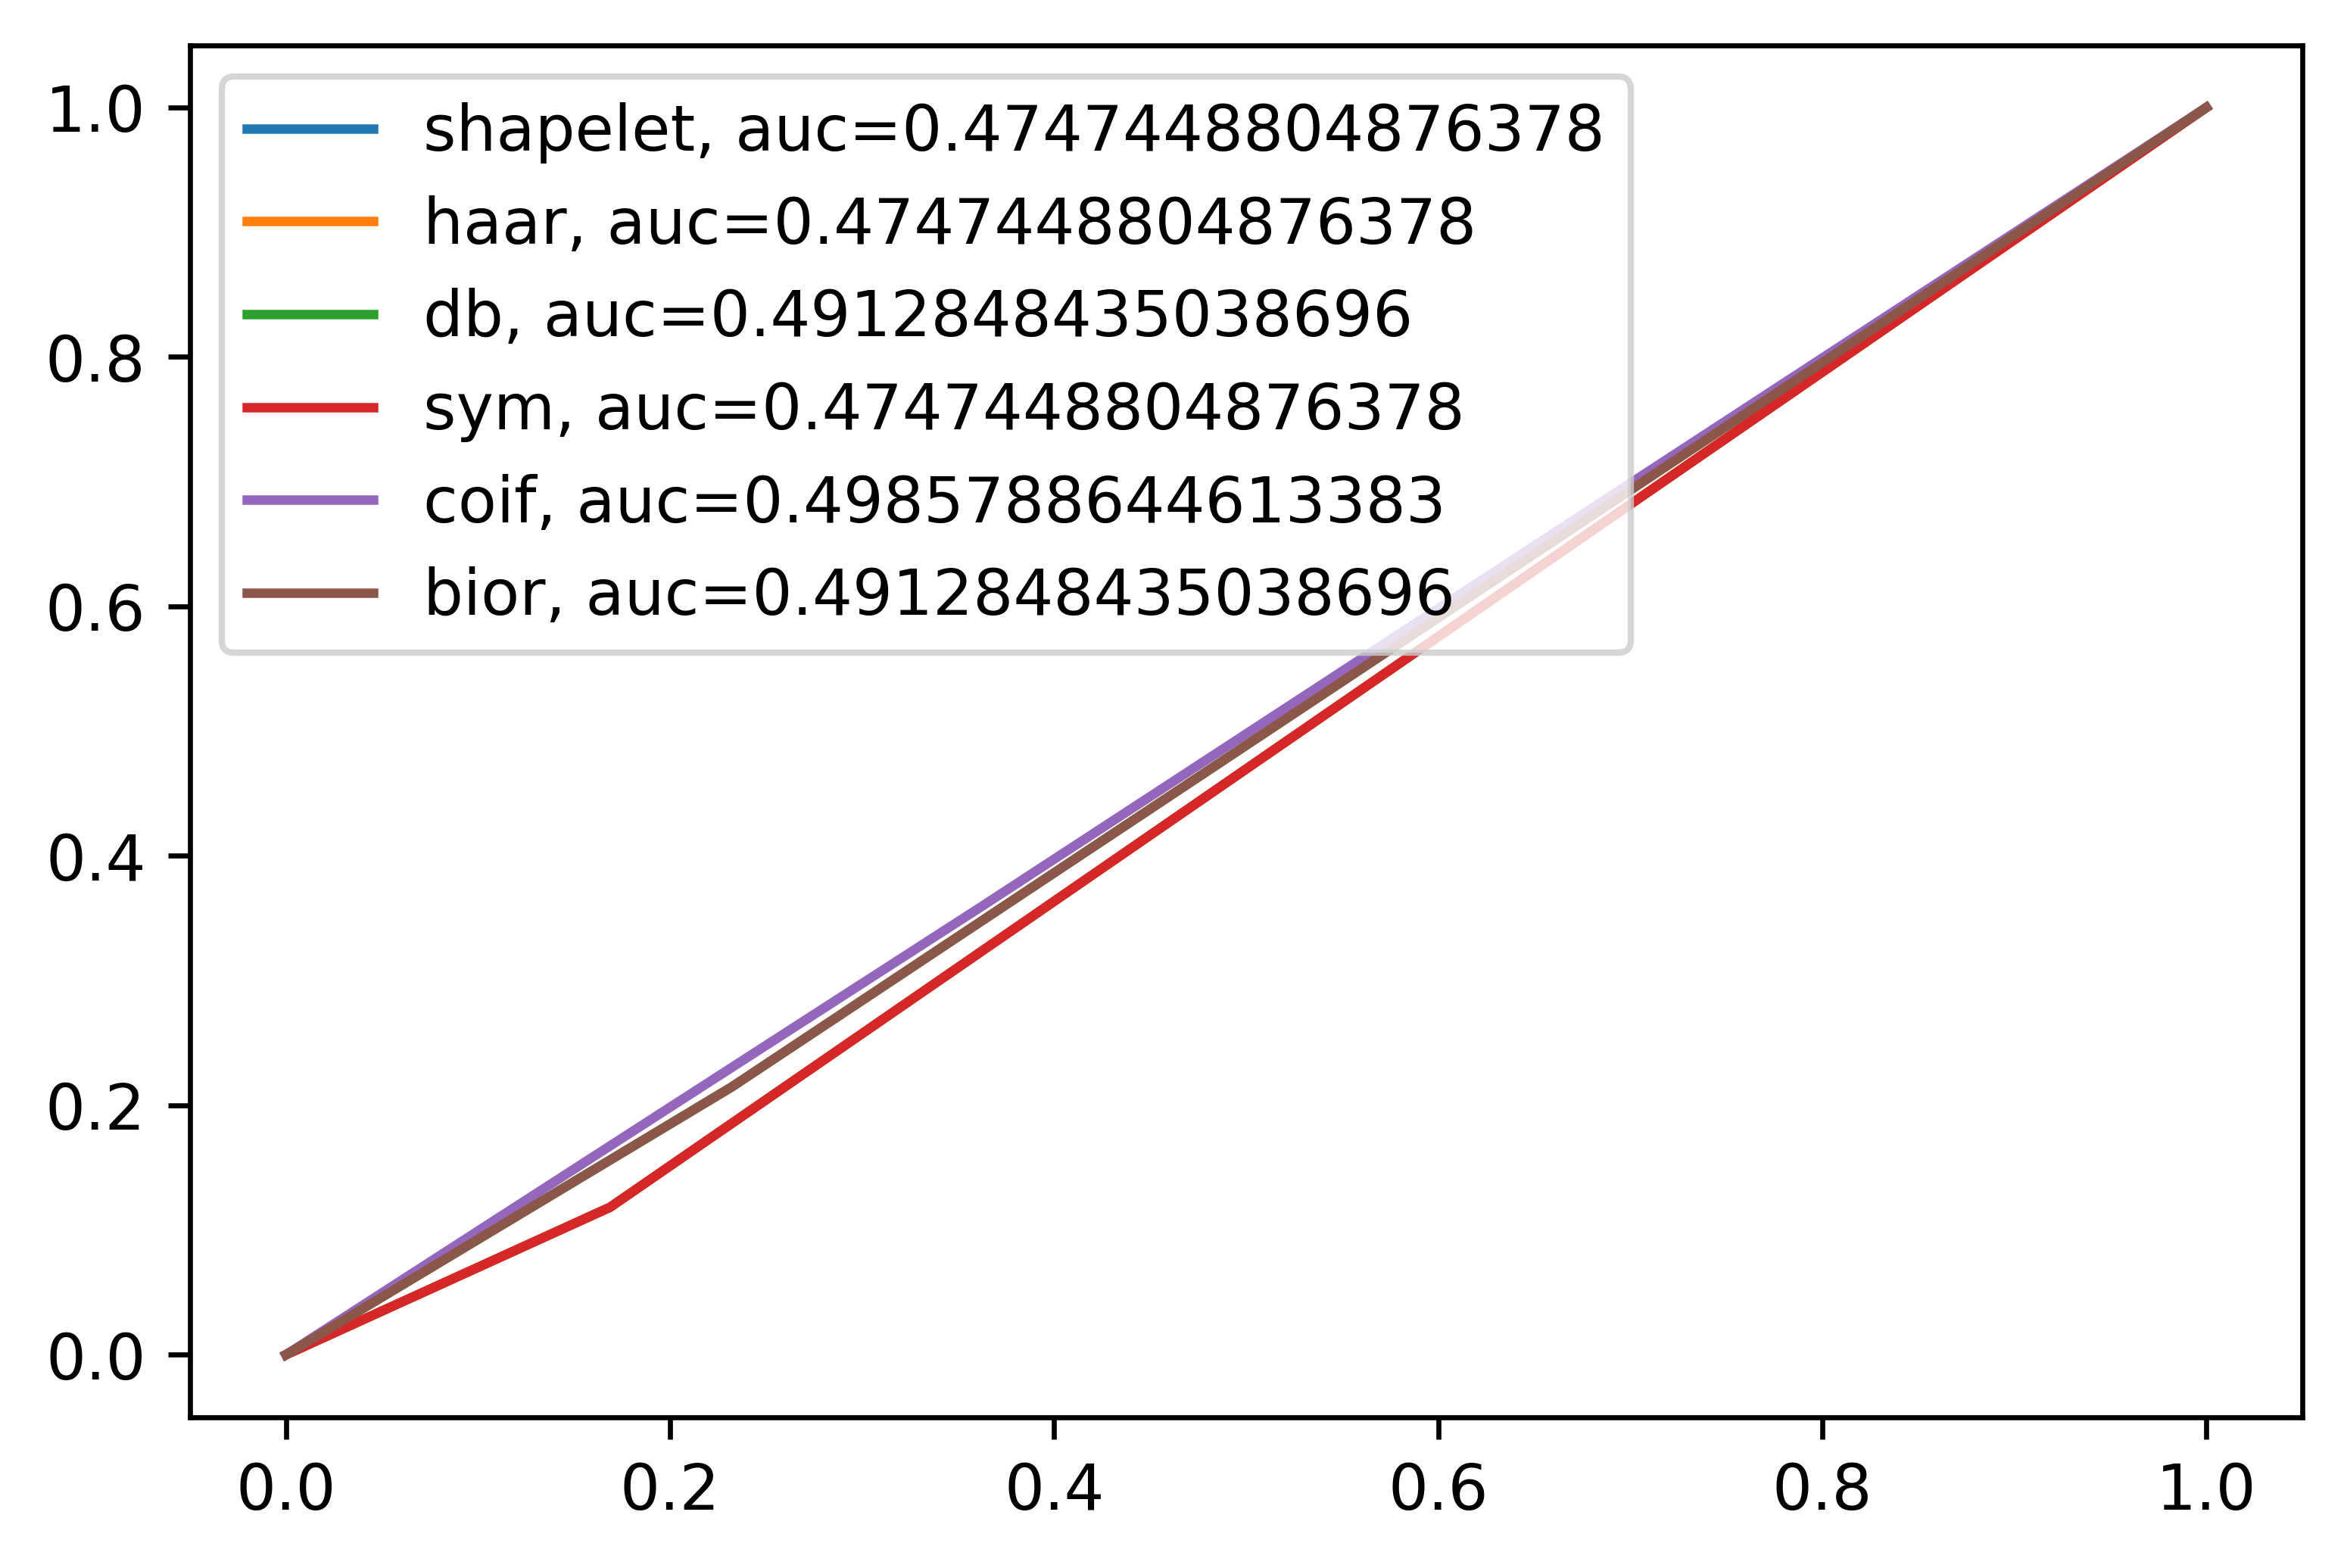
\includegraphics[scale=0.5]{Graphics/roc-th-098.png}}
	\caption{Matriz de confusión y curva ROC. En este ejemplo se tomó como umbral $th=0.98$ y un patrón de longitud 17.} \label{fig:1d-experiment-098}
\end{figure}

La selección del umbral $th$ para la medida $\mathbb{S}$ también es importante.
Las figuras \ref{fig:1d-experiment-060}, \ref{fig:1d-experiment-060} y \ref{fig:1d-experiment-098} muestran los resultados 
sobre un mismo patrón constituido por 17 muestras, pero variando el umbral $th$. El método numérico para la solución es el
mismo: Levenberg-Marquardt.

Seleccionando un umbral $th=0.6$, permite al algoritmo sacarle provecho a su capacidad de detectar el patrón. Sin embargo,
sigue habiendo una gran cantidad de falsos positivos. Si se aumenta este umbral a $th=0.85$ este número
disminuye considerablemente, pues de 216 pasa a ser tan solo 53. Como consecuencia de esto, el área debajo de la curva
(\textit{auc}) llega a alcanzar $0.90$, lo cual es un resultado sumamente bueno para un clasificador binario.

Si se sigue aumentando el umbral, esta vez a $0.98$, los resultados cambian drásticamente. La \textit{shapelet} no
se comporta para nada distinto al resto de las wavelets. Aunque teóricamente un valor igual a cero en $\mathbb{S}$ indica
la detección exacta del patrón, siempre existe un error durante el cálculo del filtro $q[\cdot]$ que impide que esto sea
cierto en la práctica. Por este motivo, poner el umbral de detección demasiado alto empeora los resultados.
Por lo tanto, un valor entre $0.6$ (valor que recomiendan en \cite{Guido2018}) y $0.90$ se considera idóneo.


\begin{figure}
	\centering
	\subfigure[Patrón]{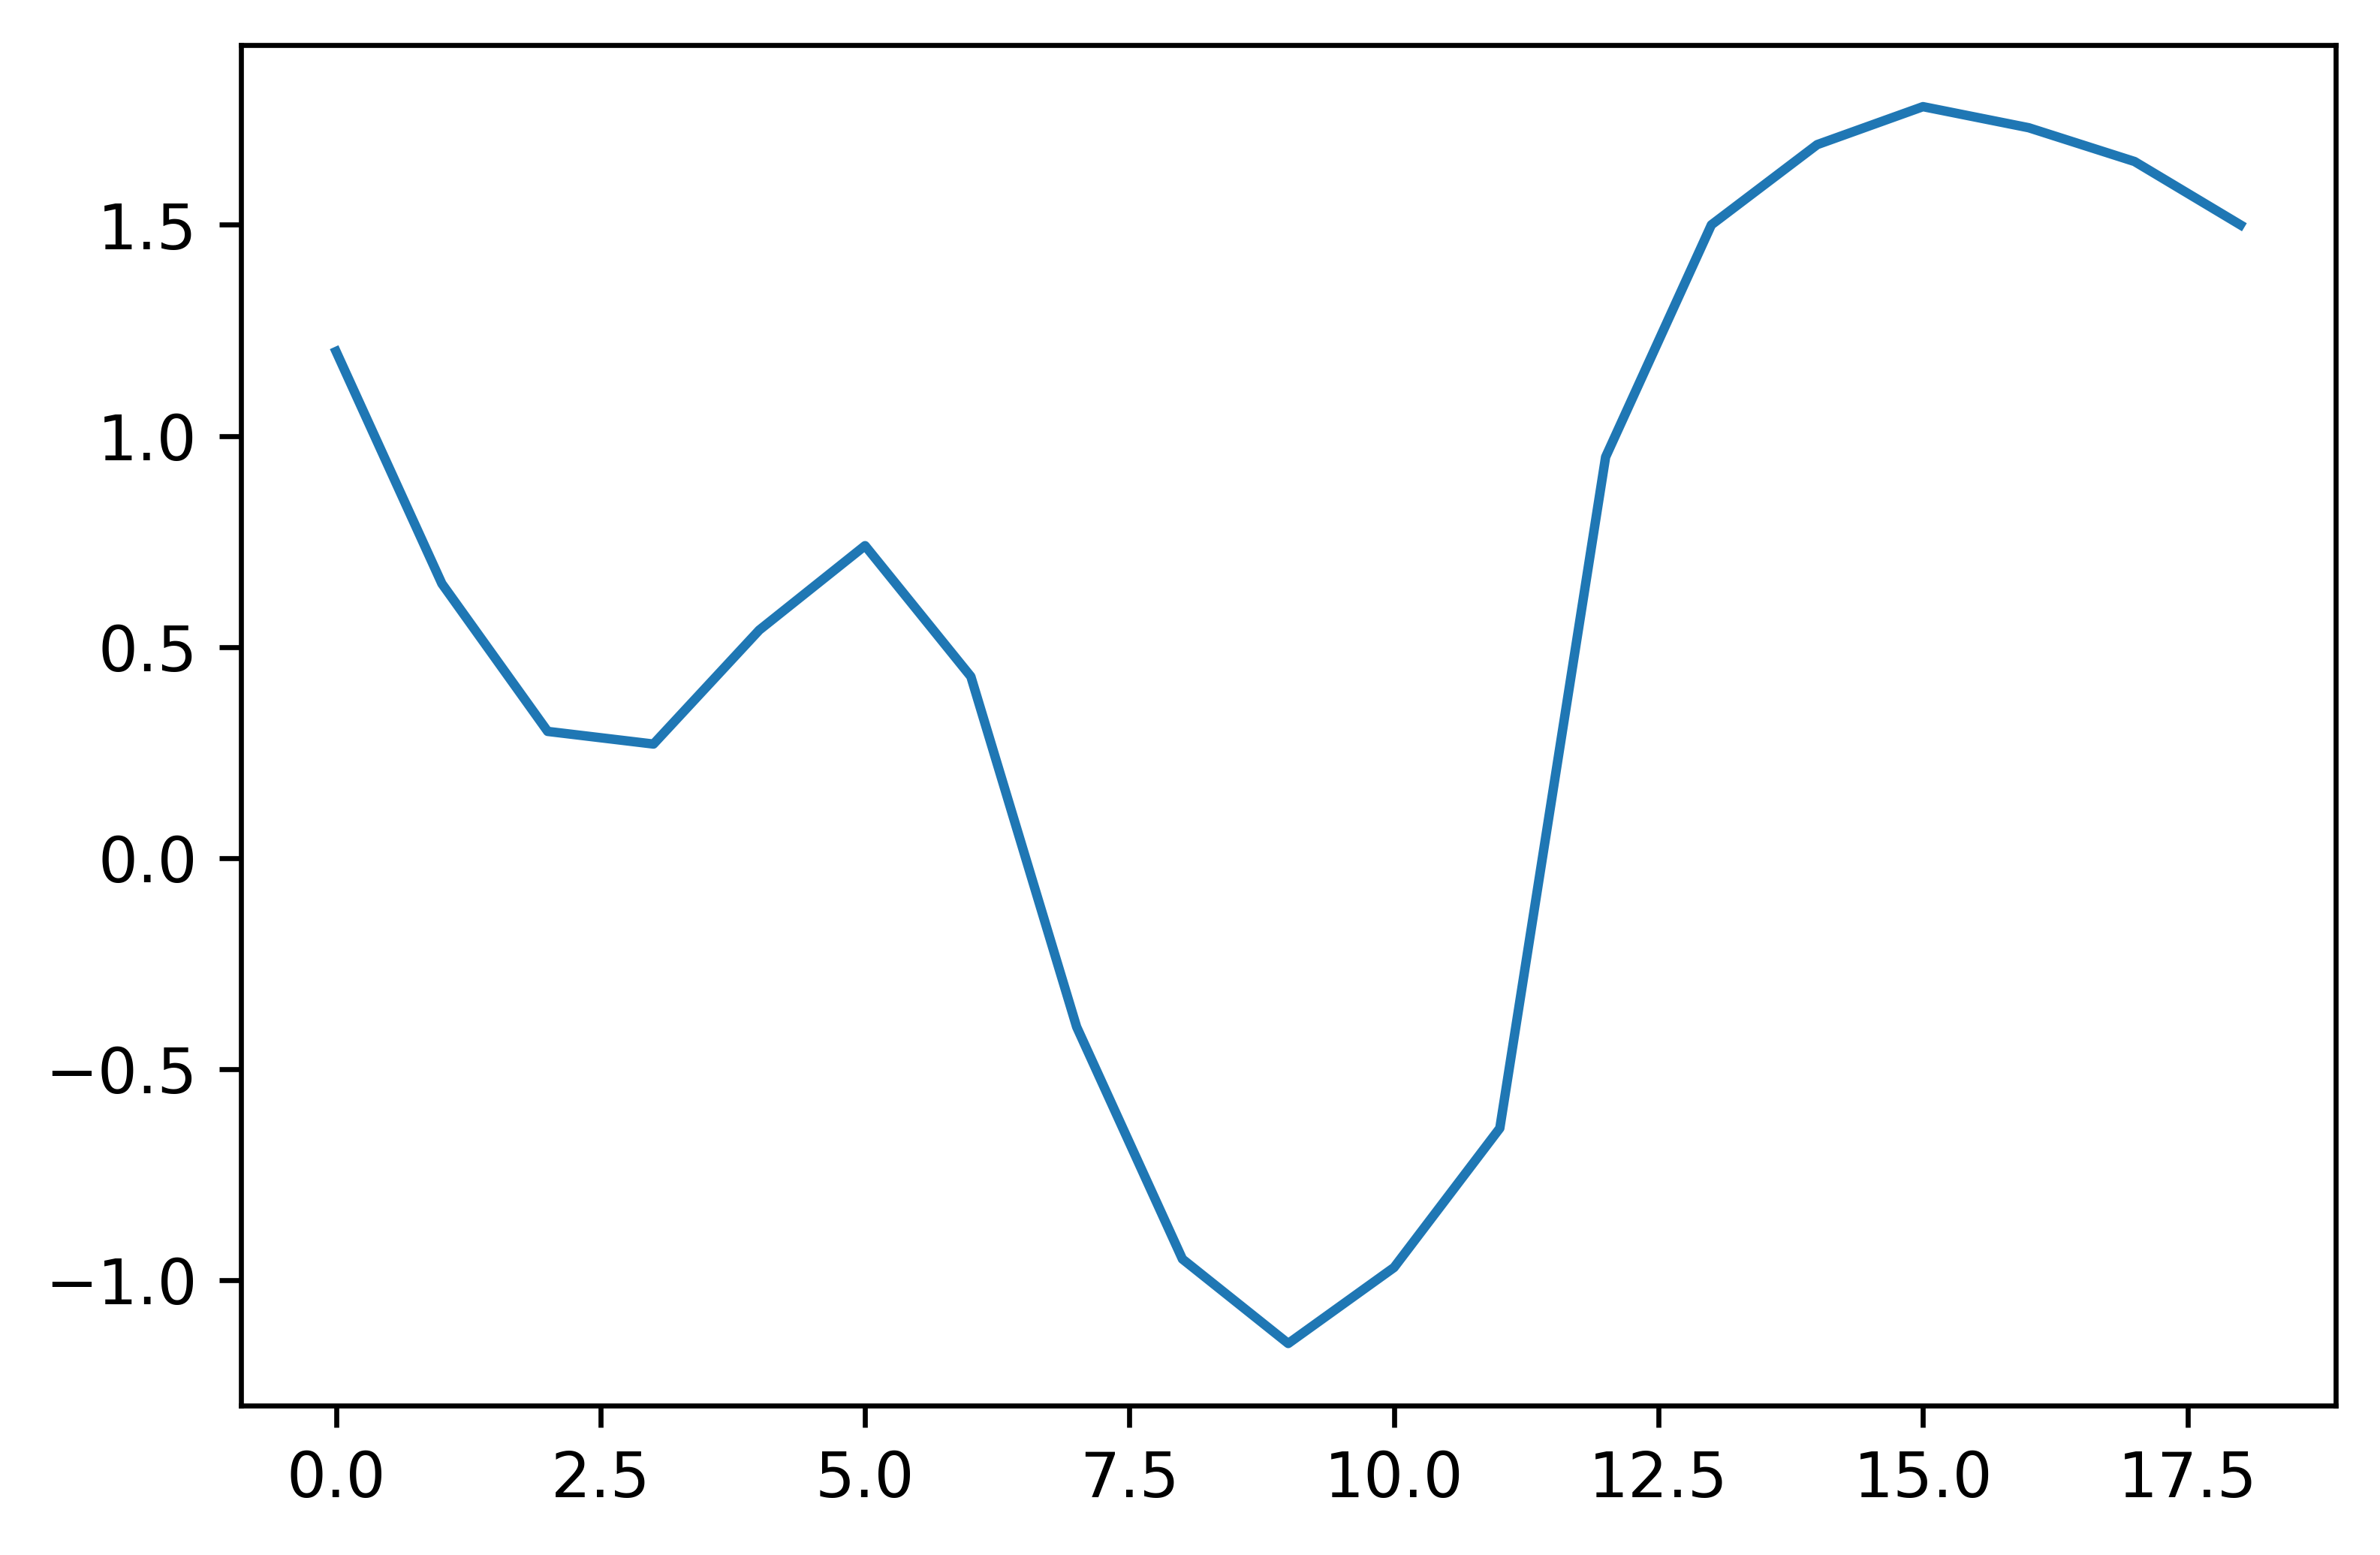
\includegraphics[scale=0.5]{Graphics/success-example-pattern.png}}
	\subfigure[Señal con patrón insertado]{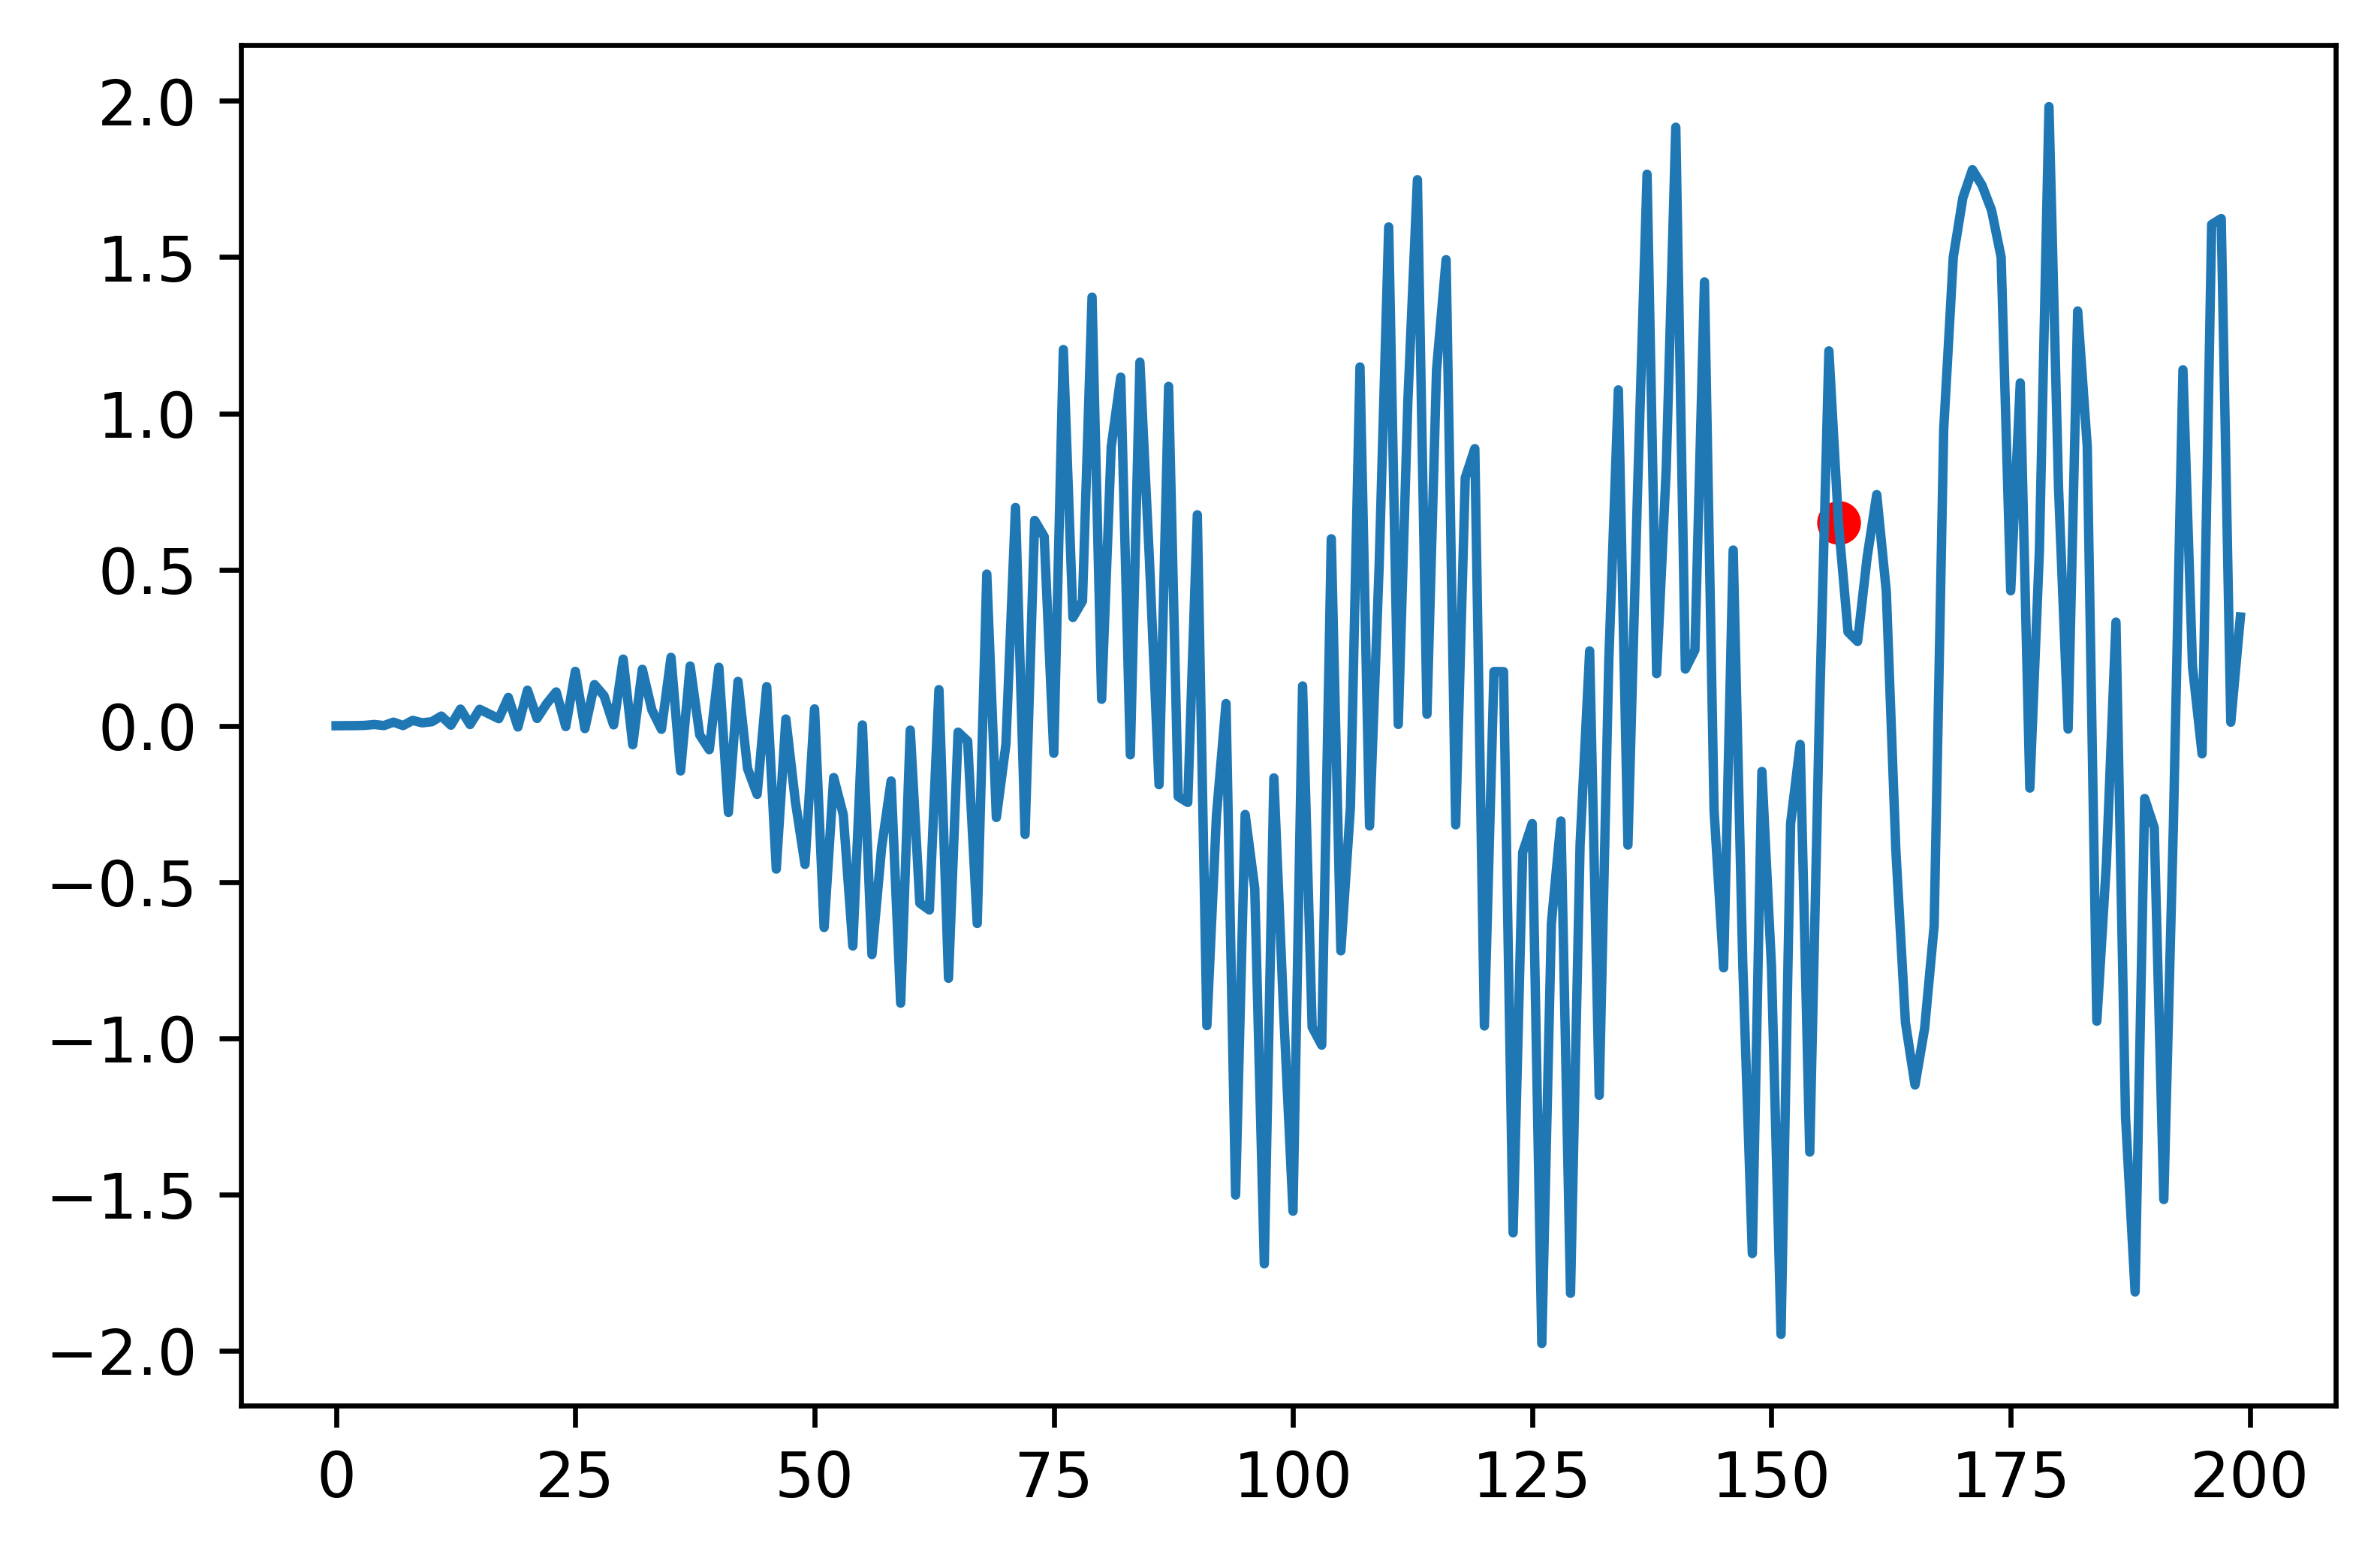
\includegraphics[scale=0.5]{Graphics/success-example-signal.png}}
	\subfigure[Major shapelet]{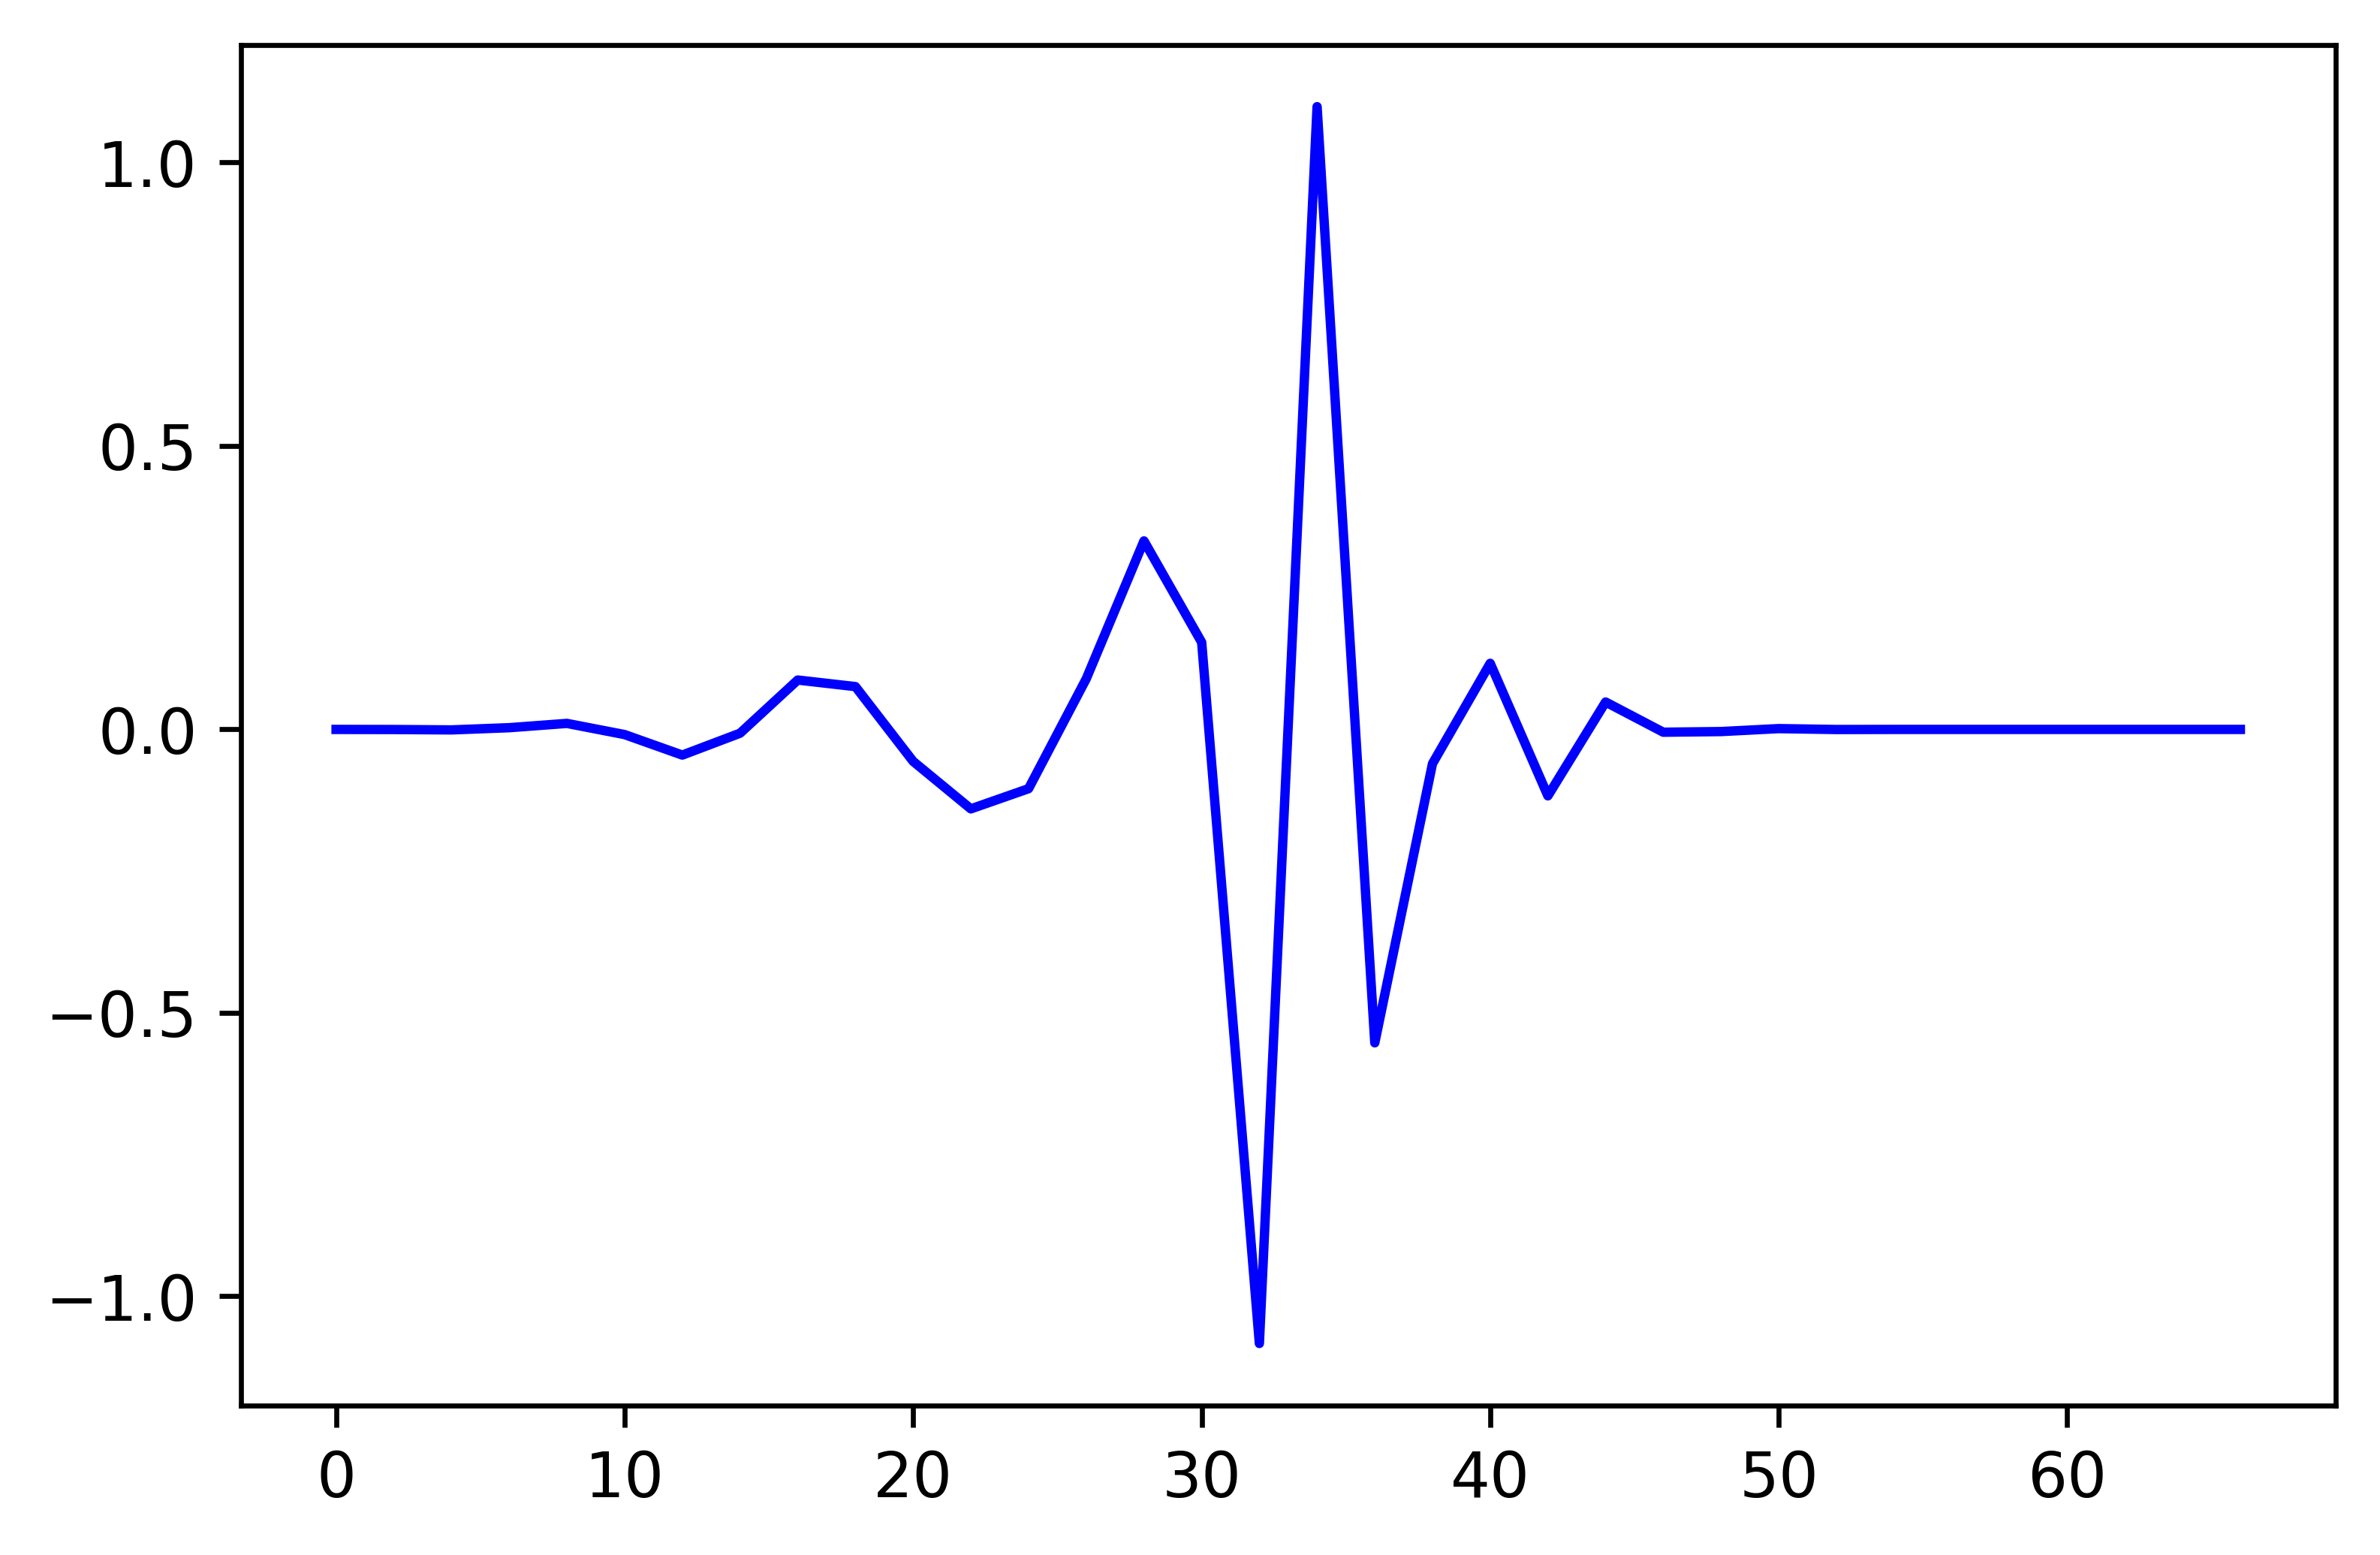
\includegraphics[scale=0.5]{Graphics/success-example-blue-shapelet.png}}
	\subfigure[Minor shapelet]{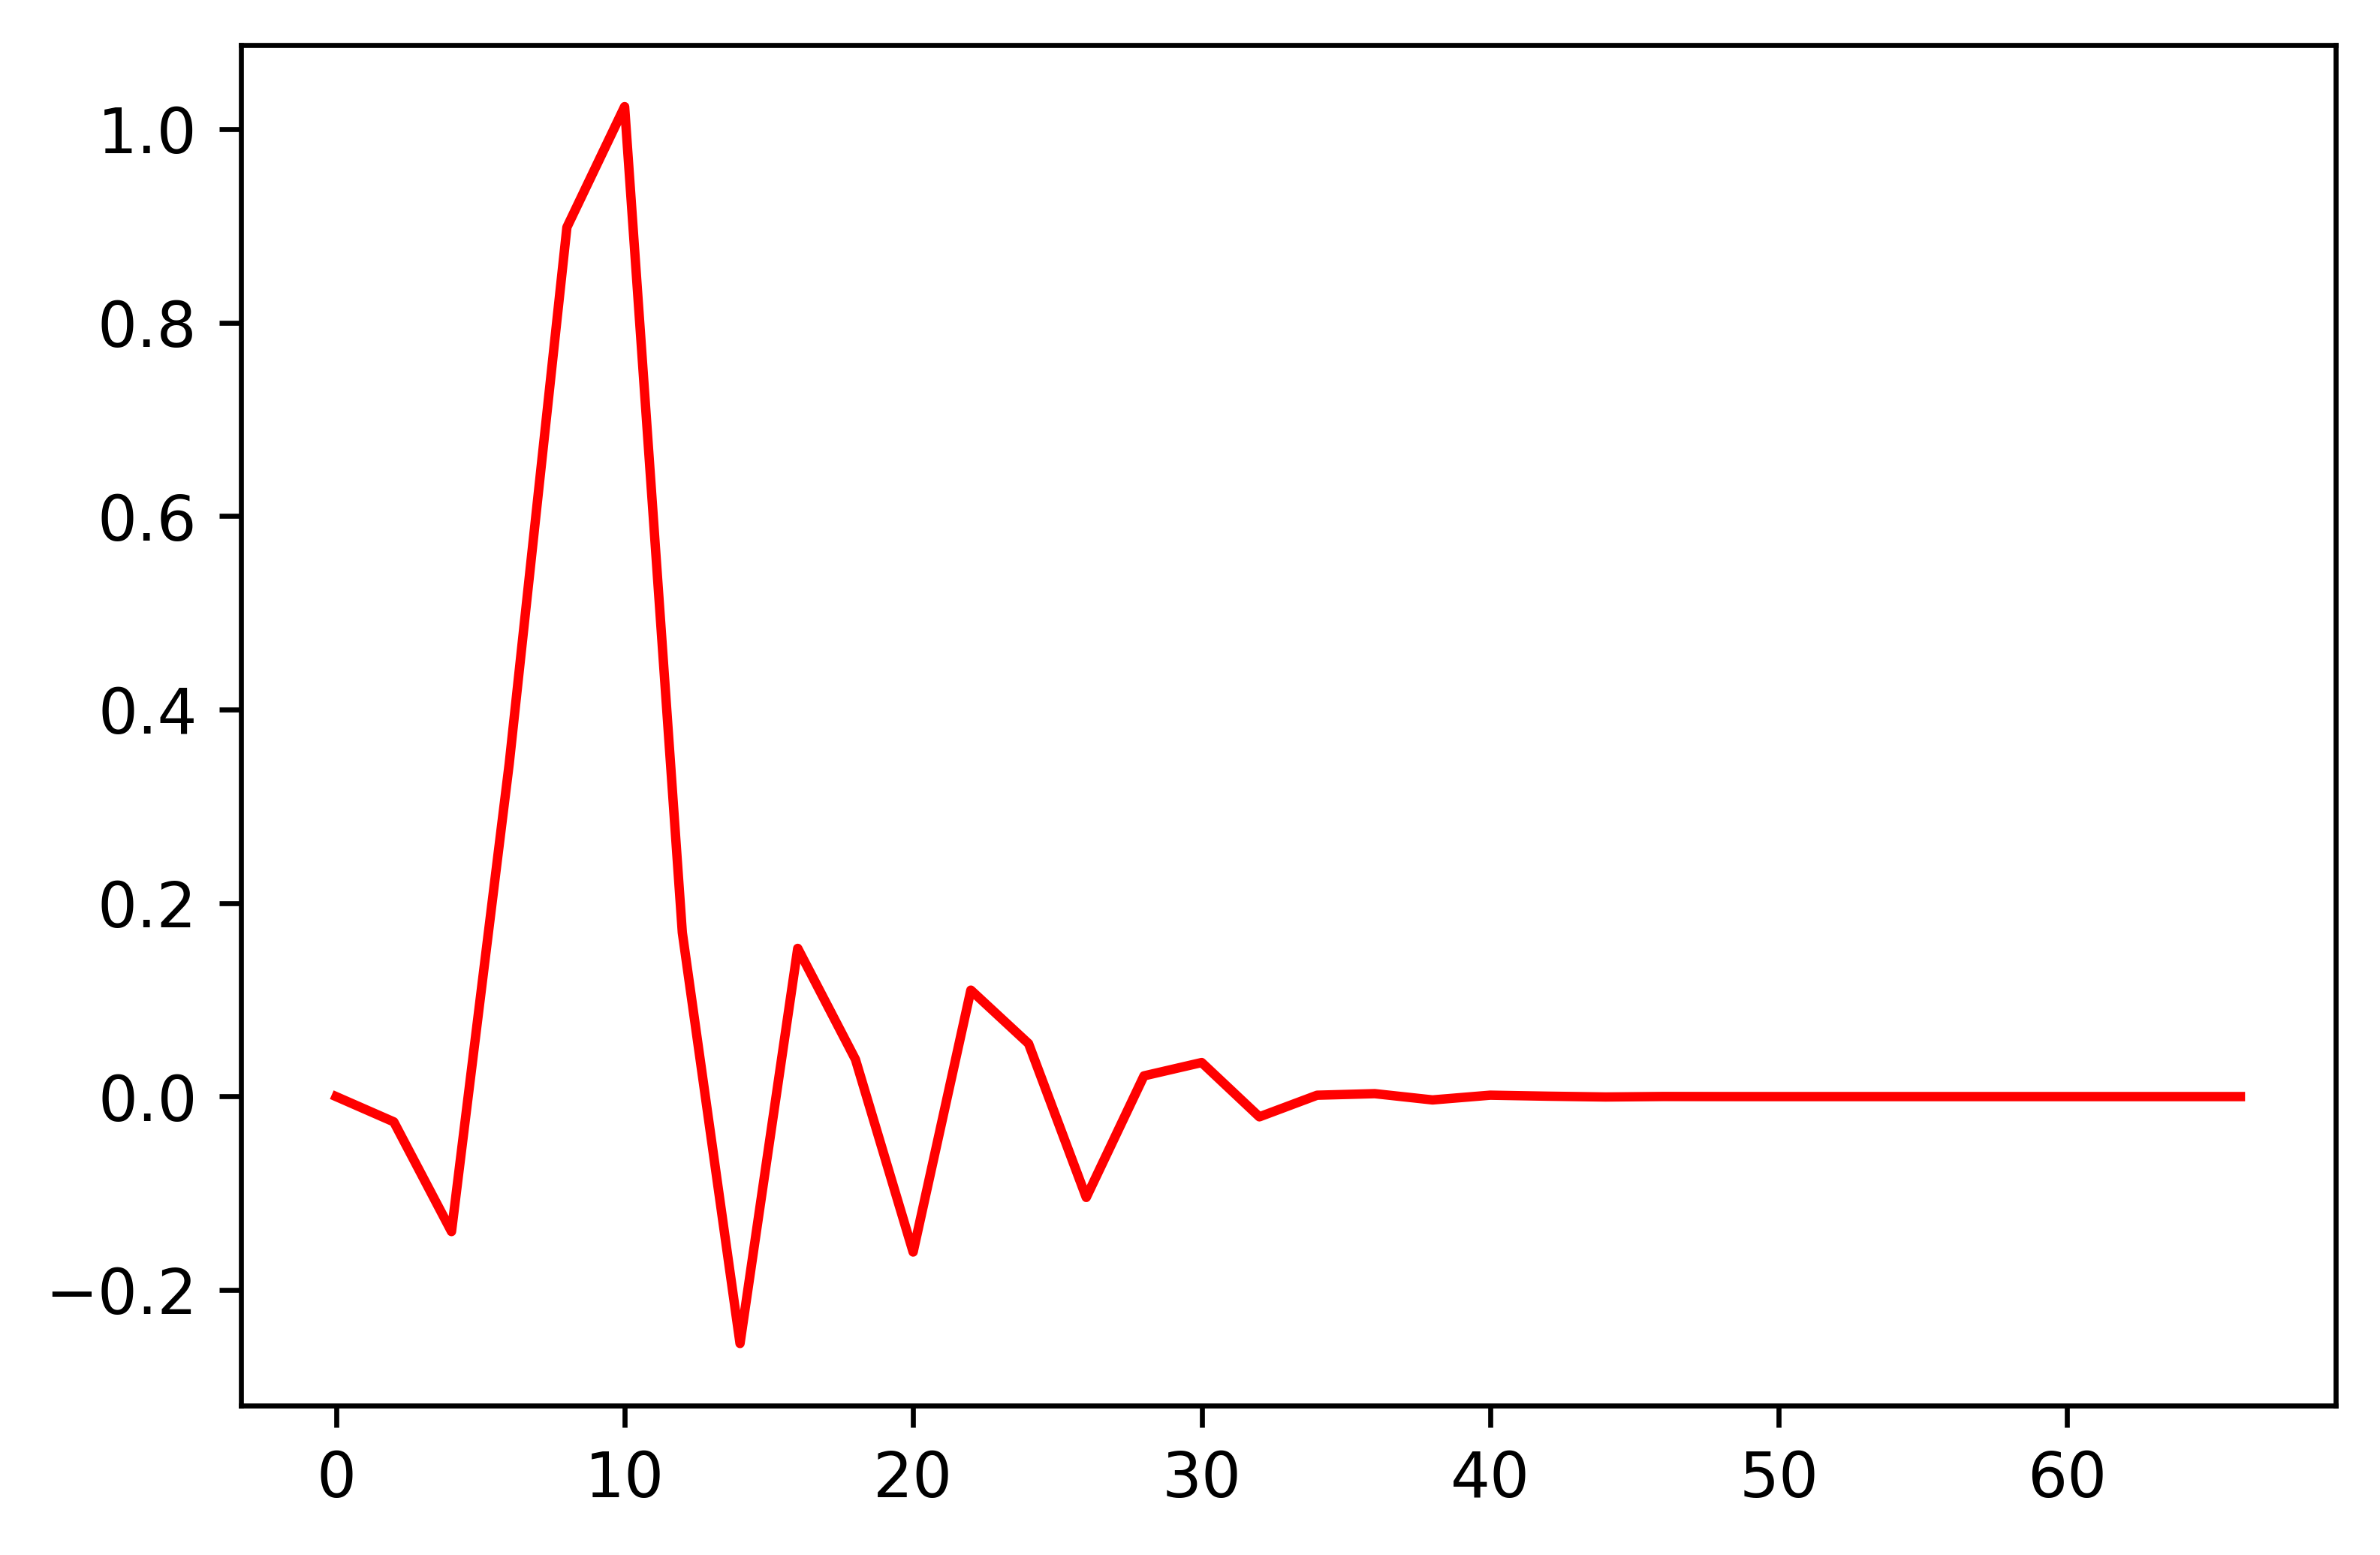
\includegraphics[scale=0.5]{Graphics/success-example-red-shapelet.png}}
	\subfigure[DST-II y medida $\mathbb{S}$]{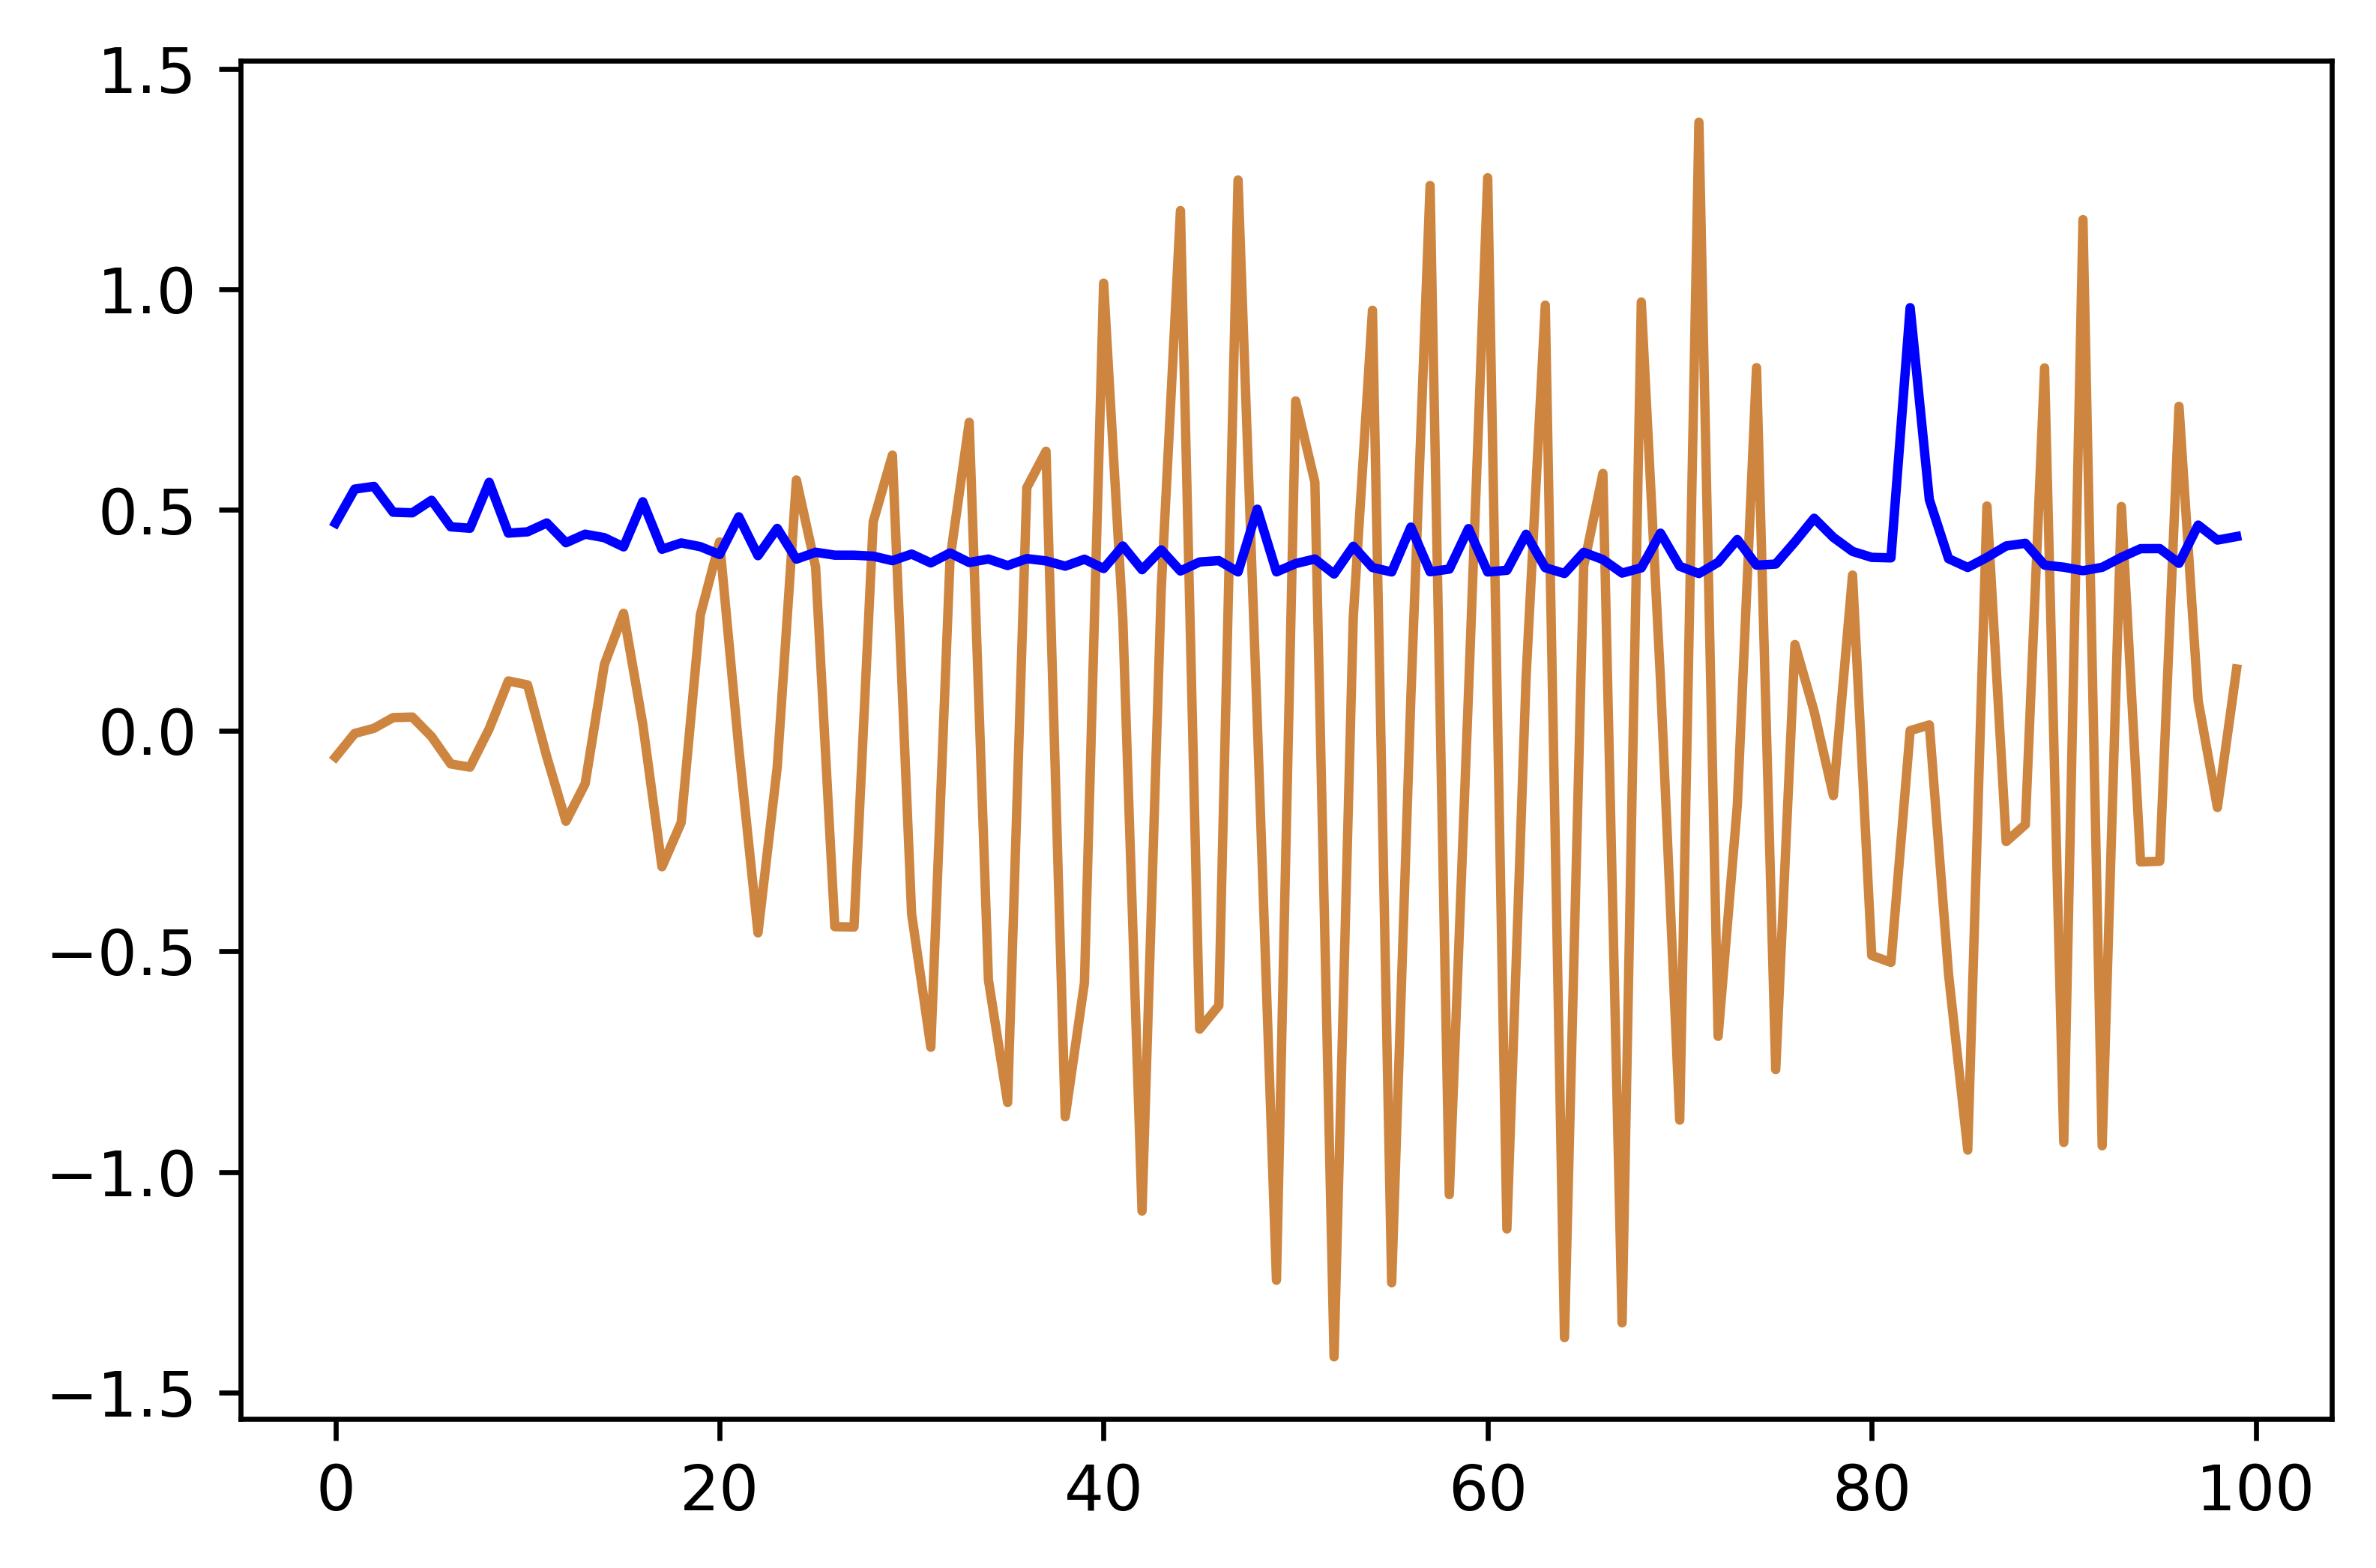
\includegraphics[scale=0.5]{Graphics/success-example-detection.png}}
	\caption{Ejemplo donde el algoritmo logra detectar la posición donde se encuentra el patrón.} \label{fig:success-example-experiment}
\end{figure}

\begin{figure}
	\centering
	\subfigure[Patrón]{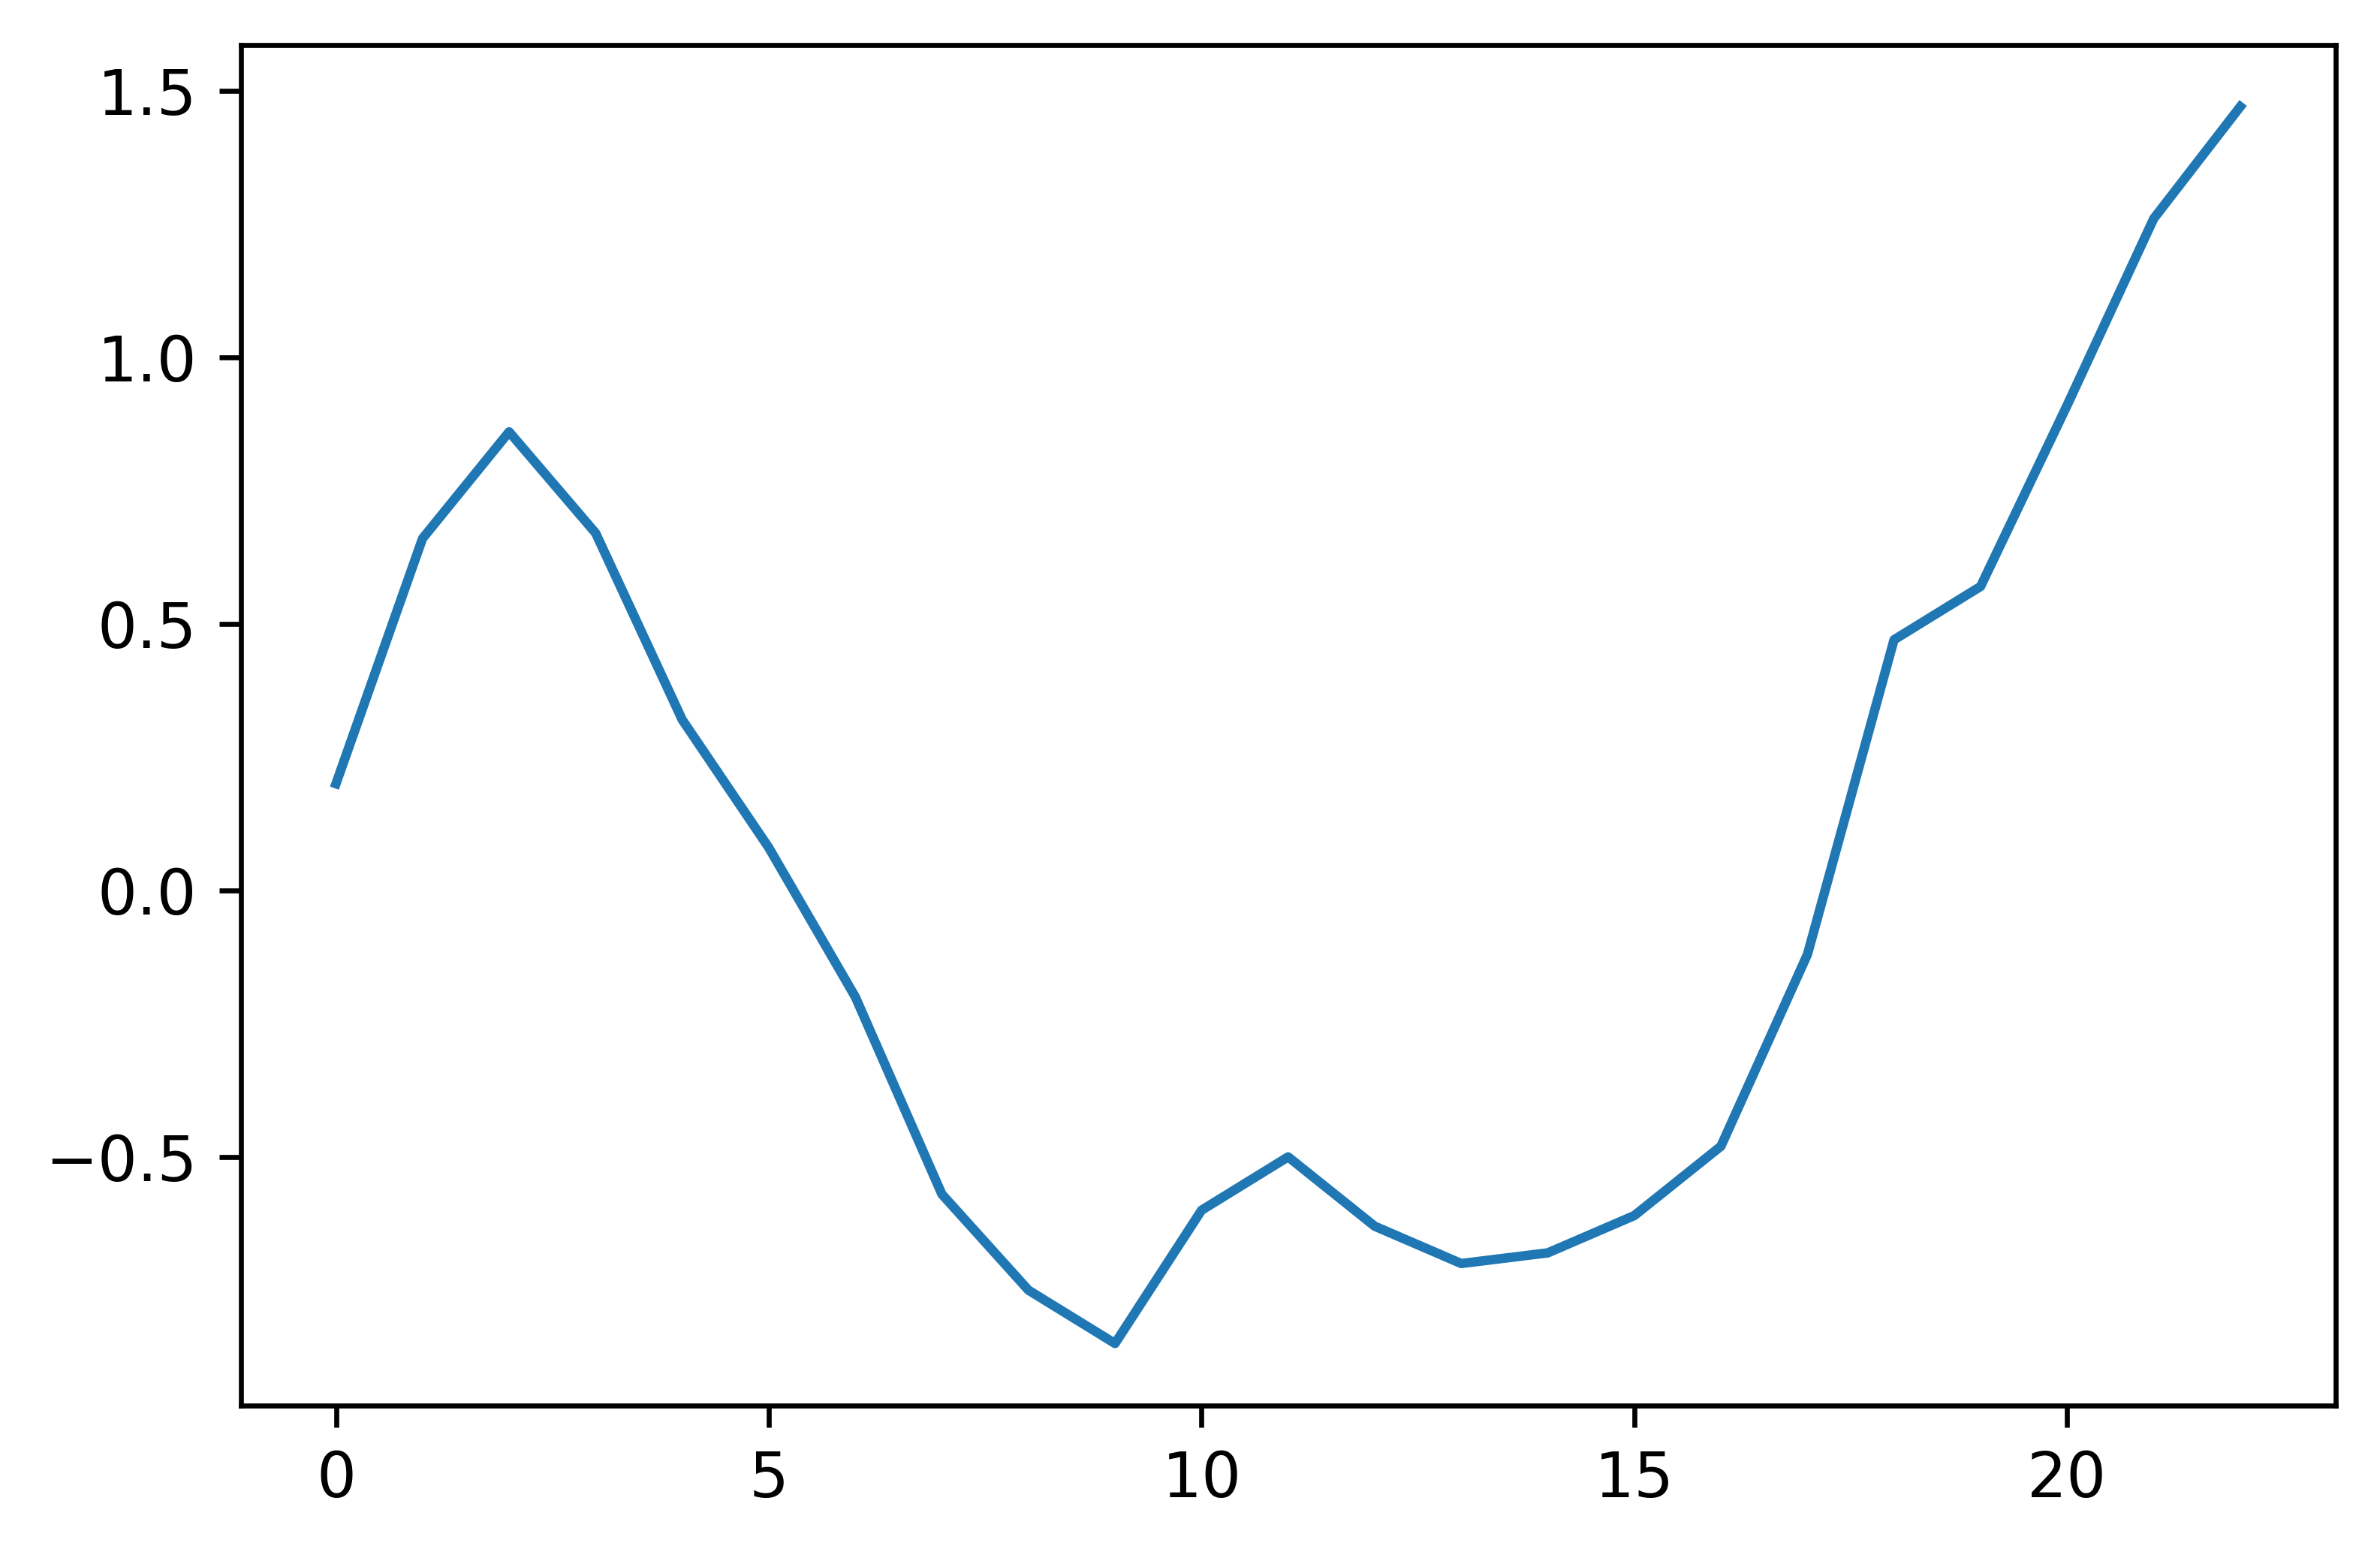
\includegraphics[scale=0.5]{Graphics/failed-example-pattern.png}}
	\subfigure[Señal con patrón insertado]{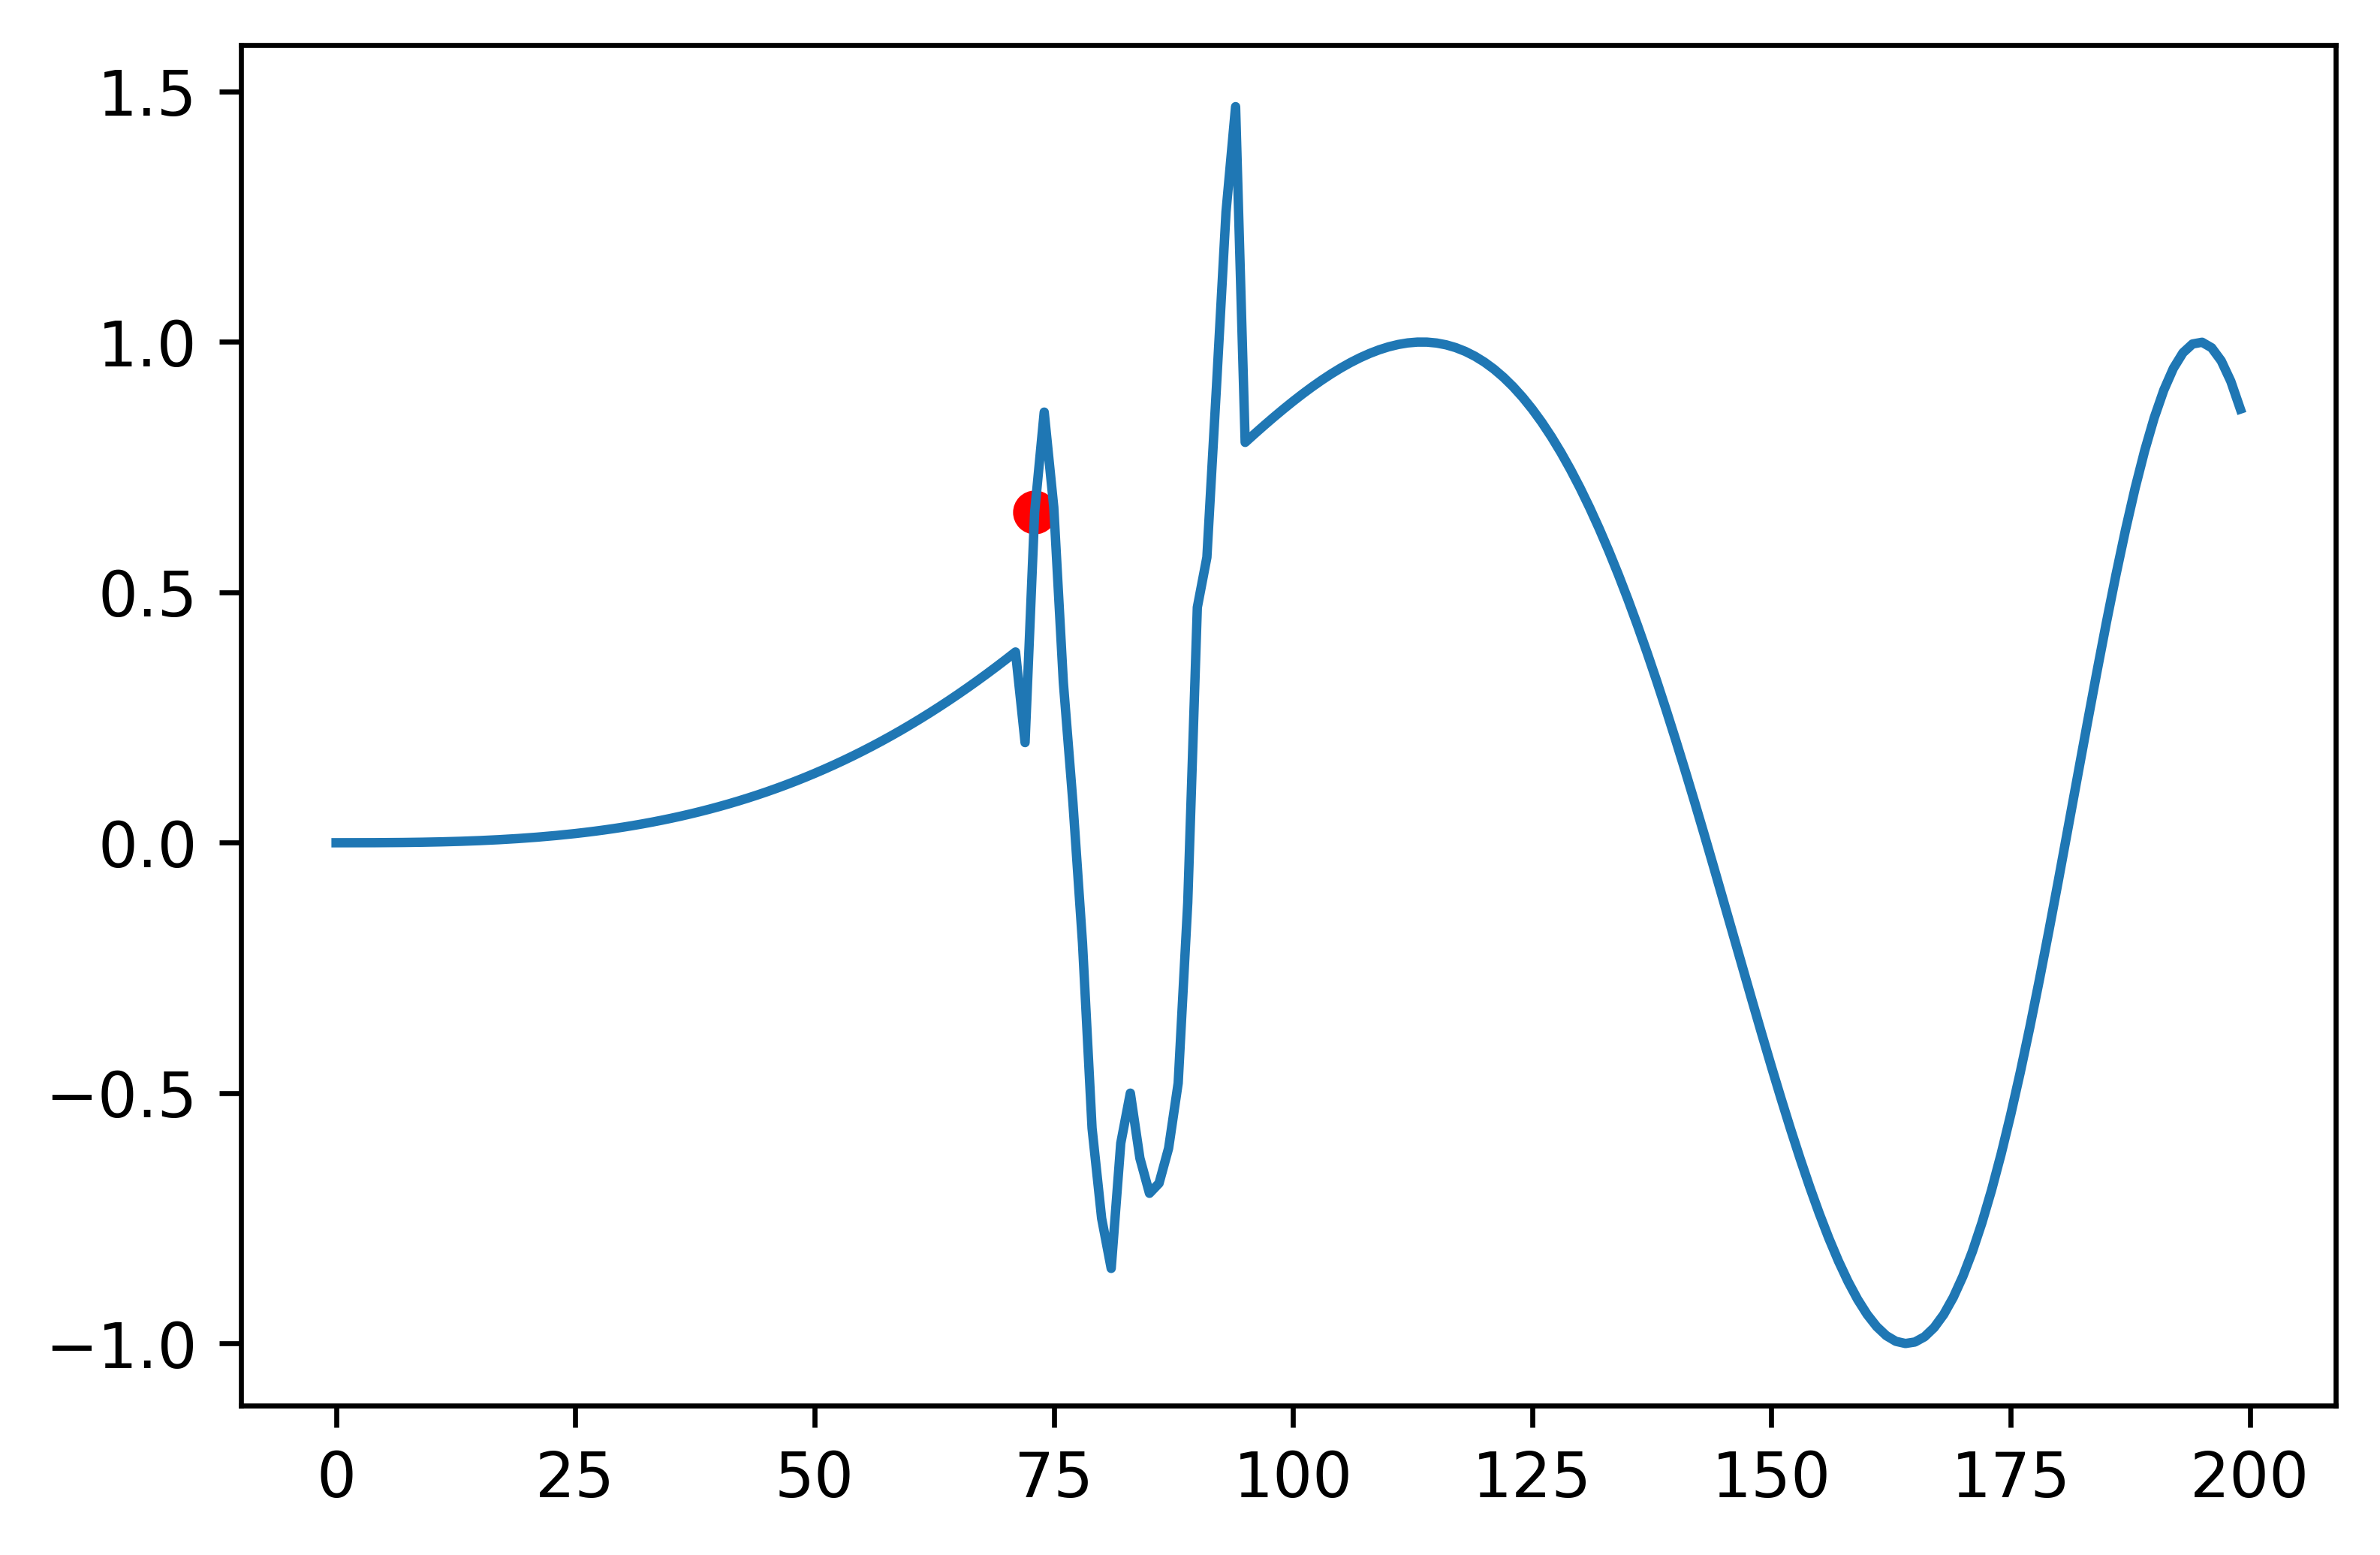
\includegraphics[scale=0.5]{Graphics/failed-example-signal.png}}
	\subfigure[Major shapelet]{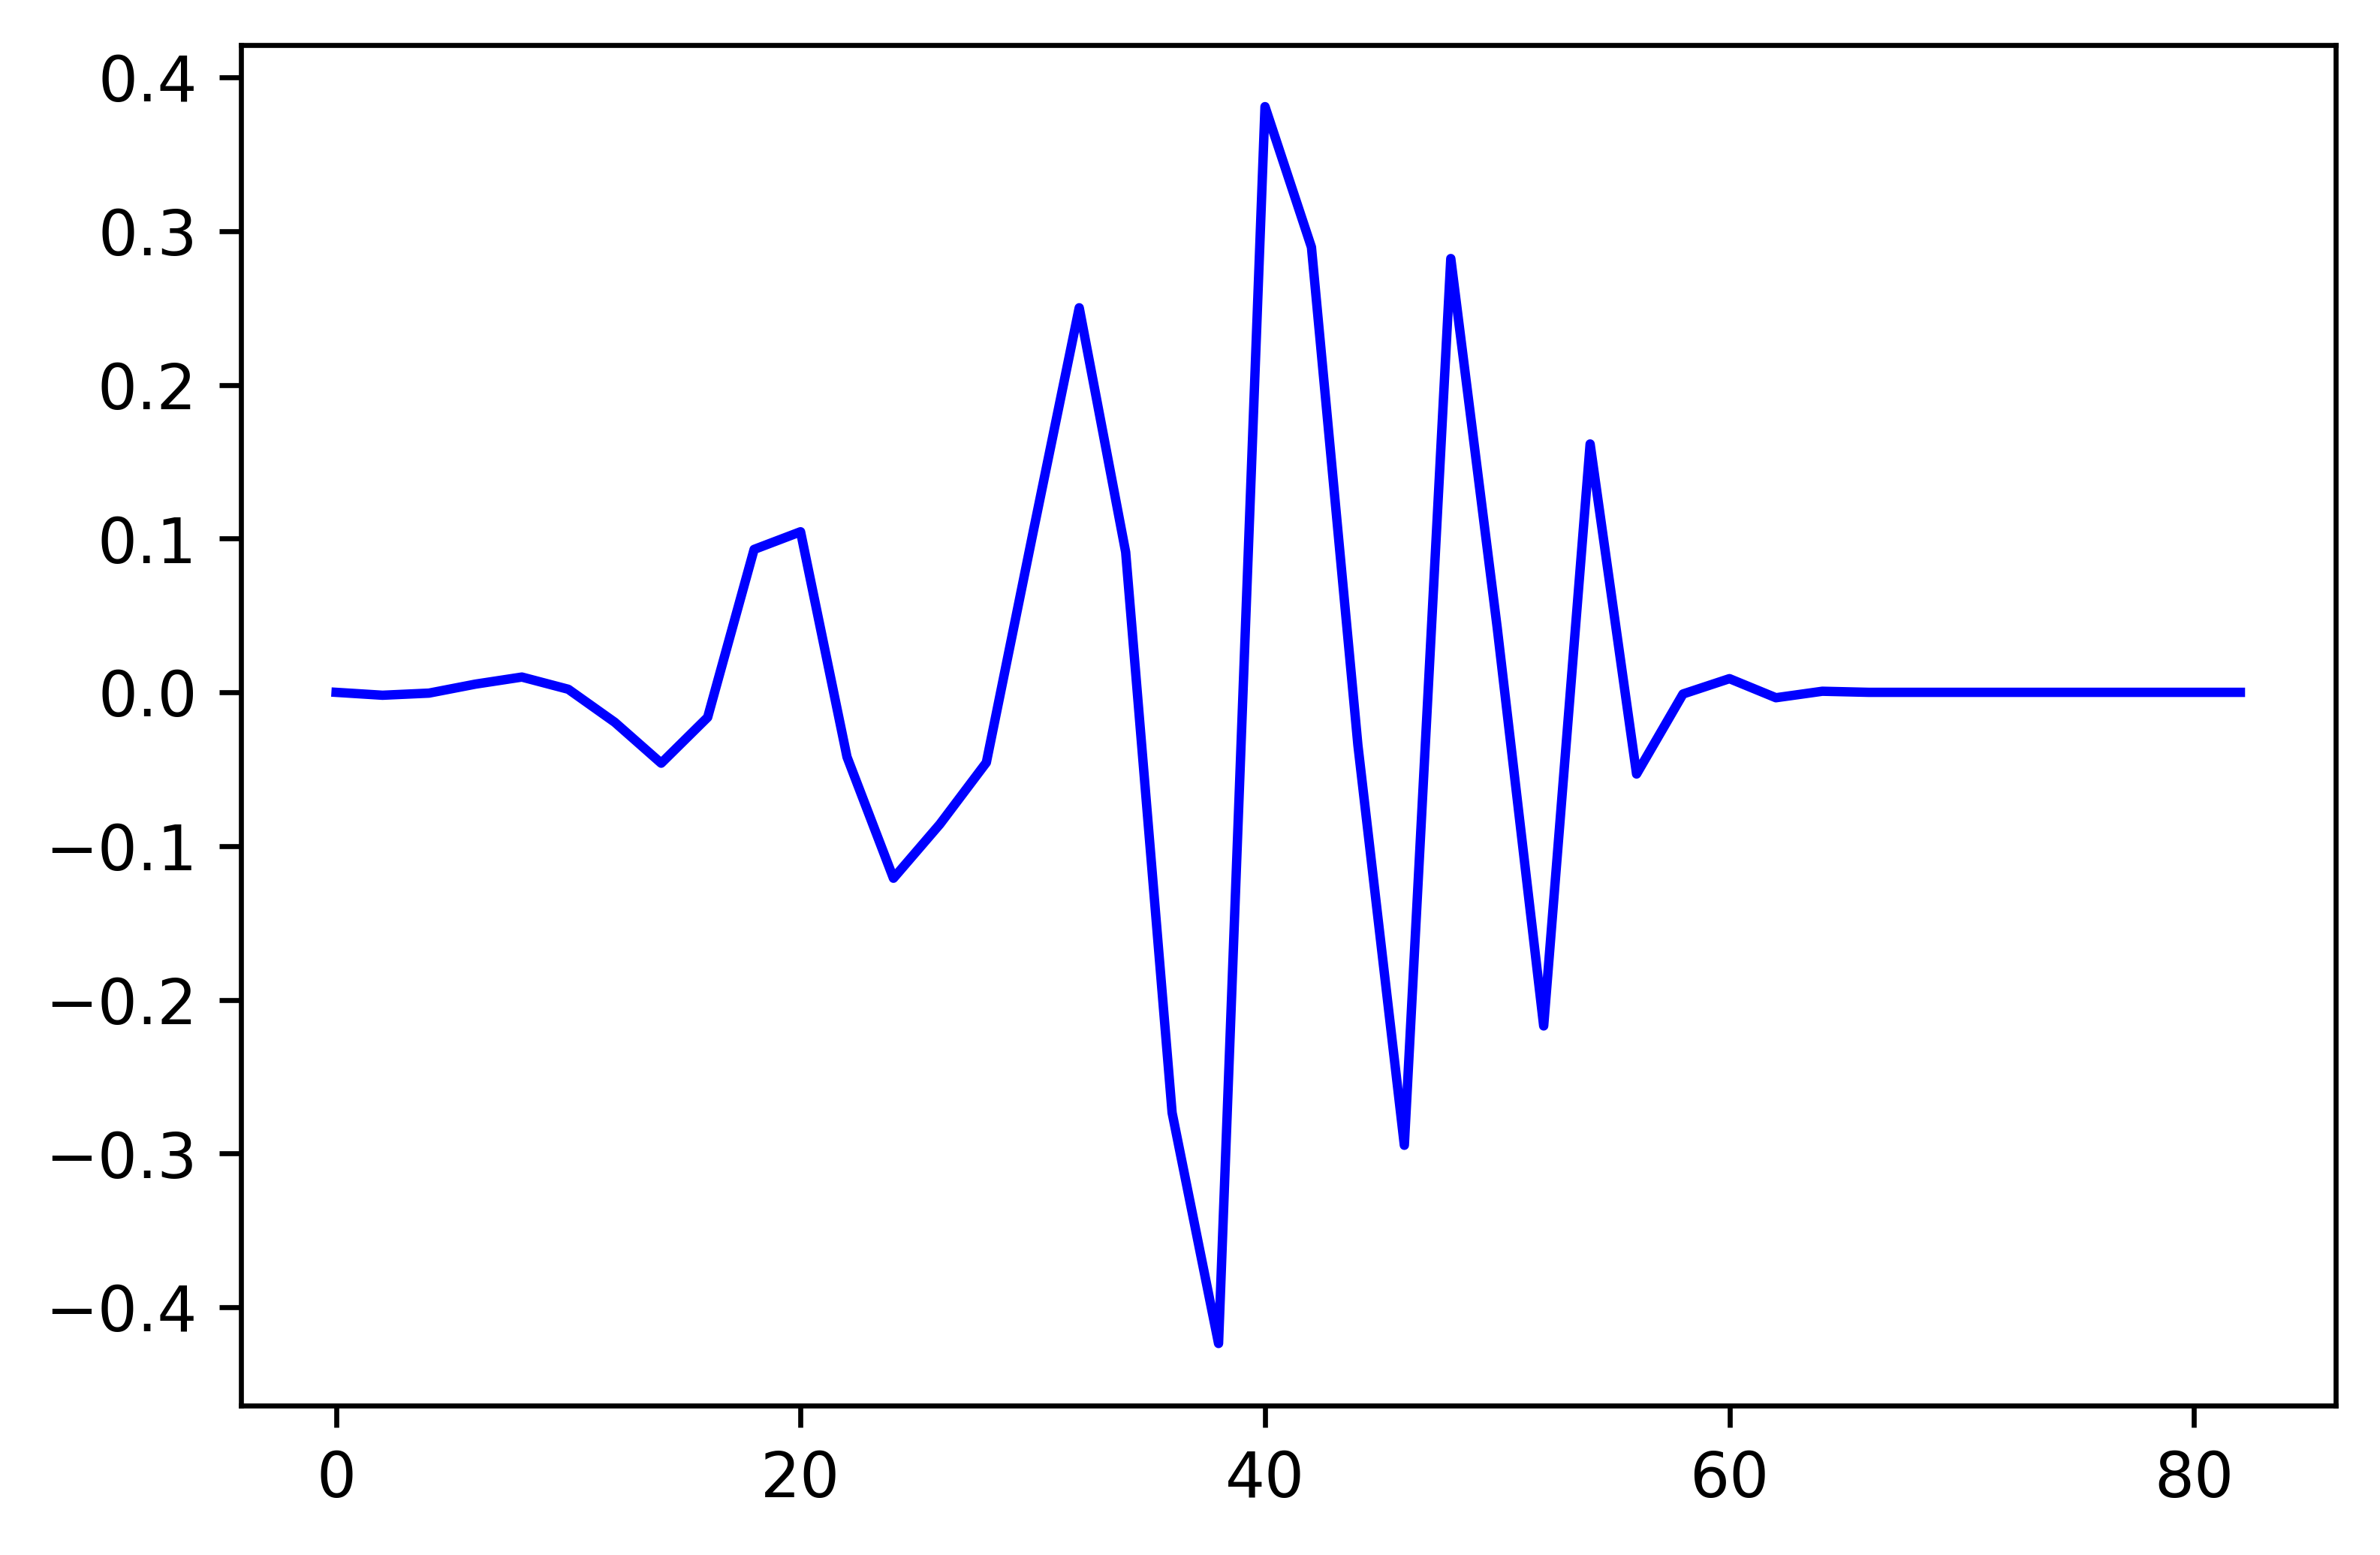
\includegraphics[scale=0.5]{Graphics/failed-example-blue-shapelet.png}}
	\subfigure[Minor shapelet]{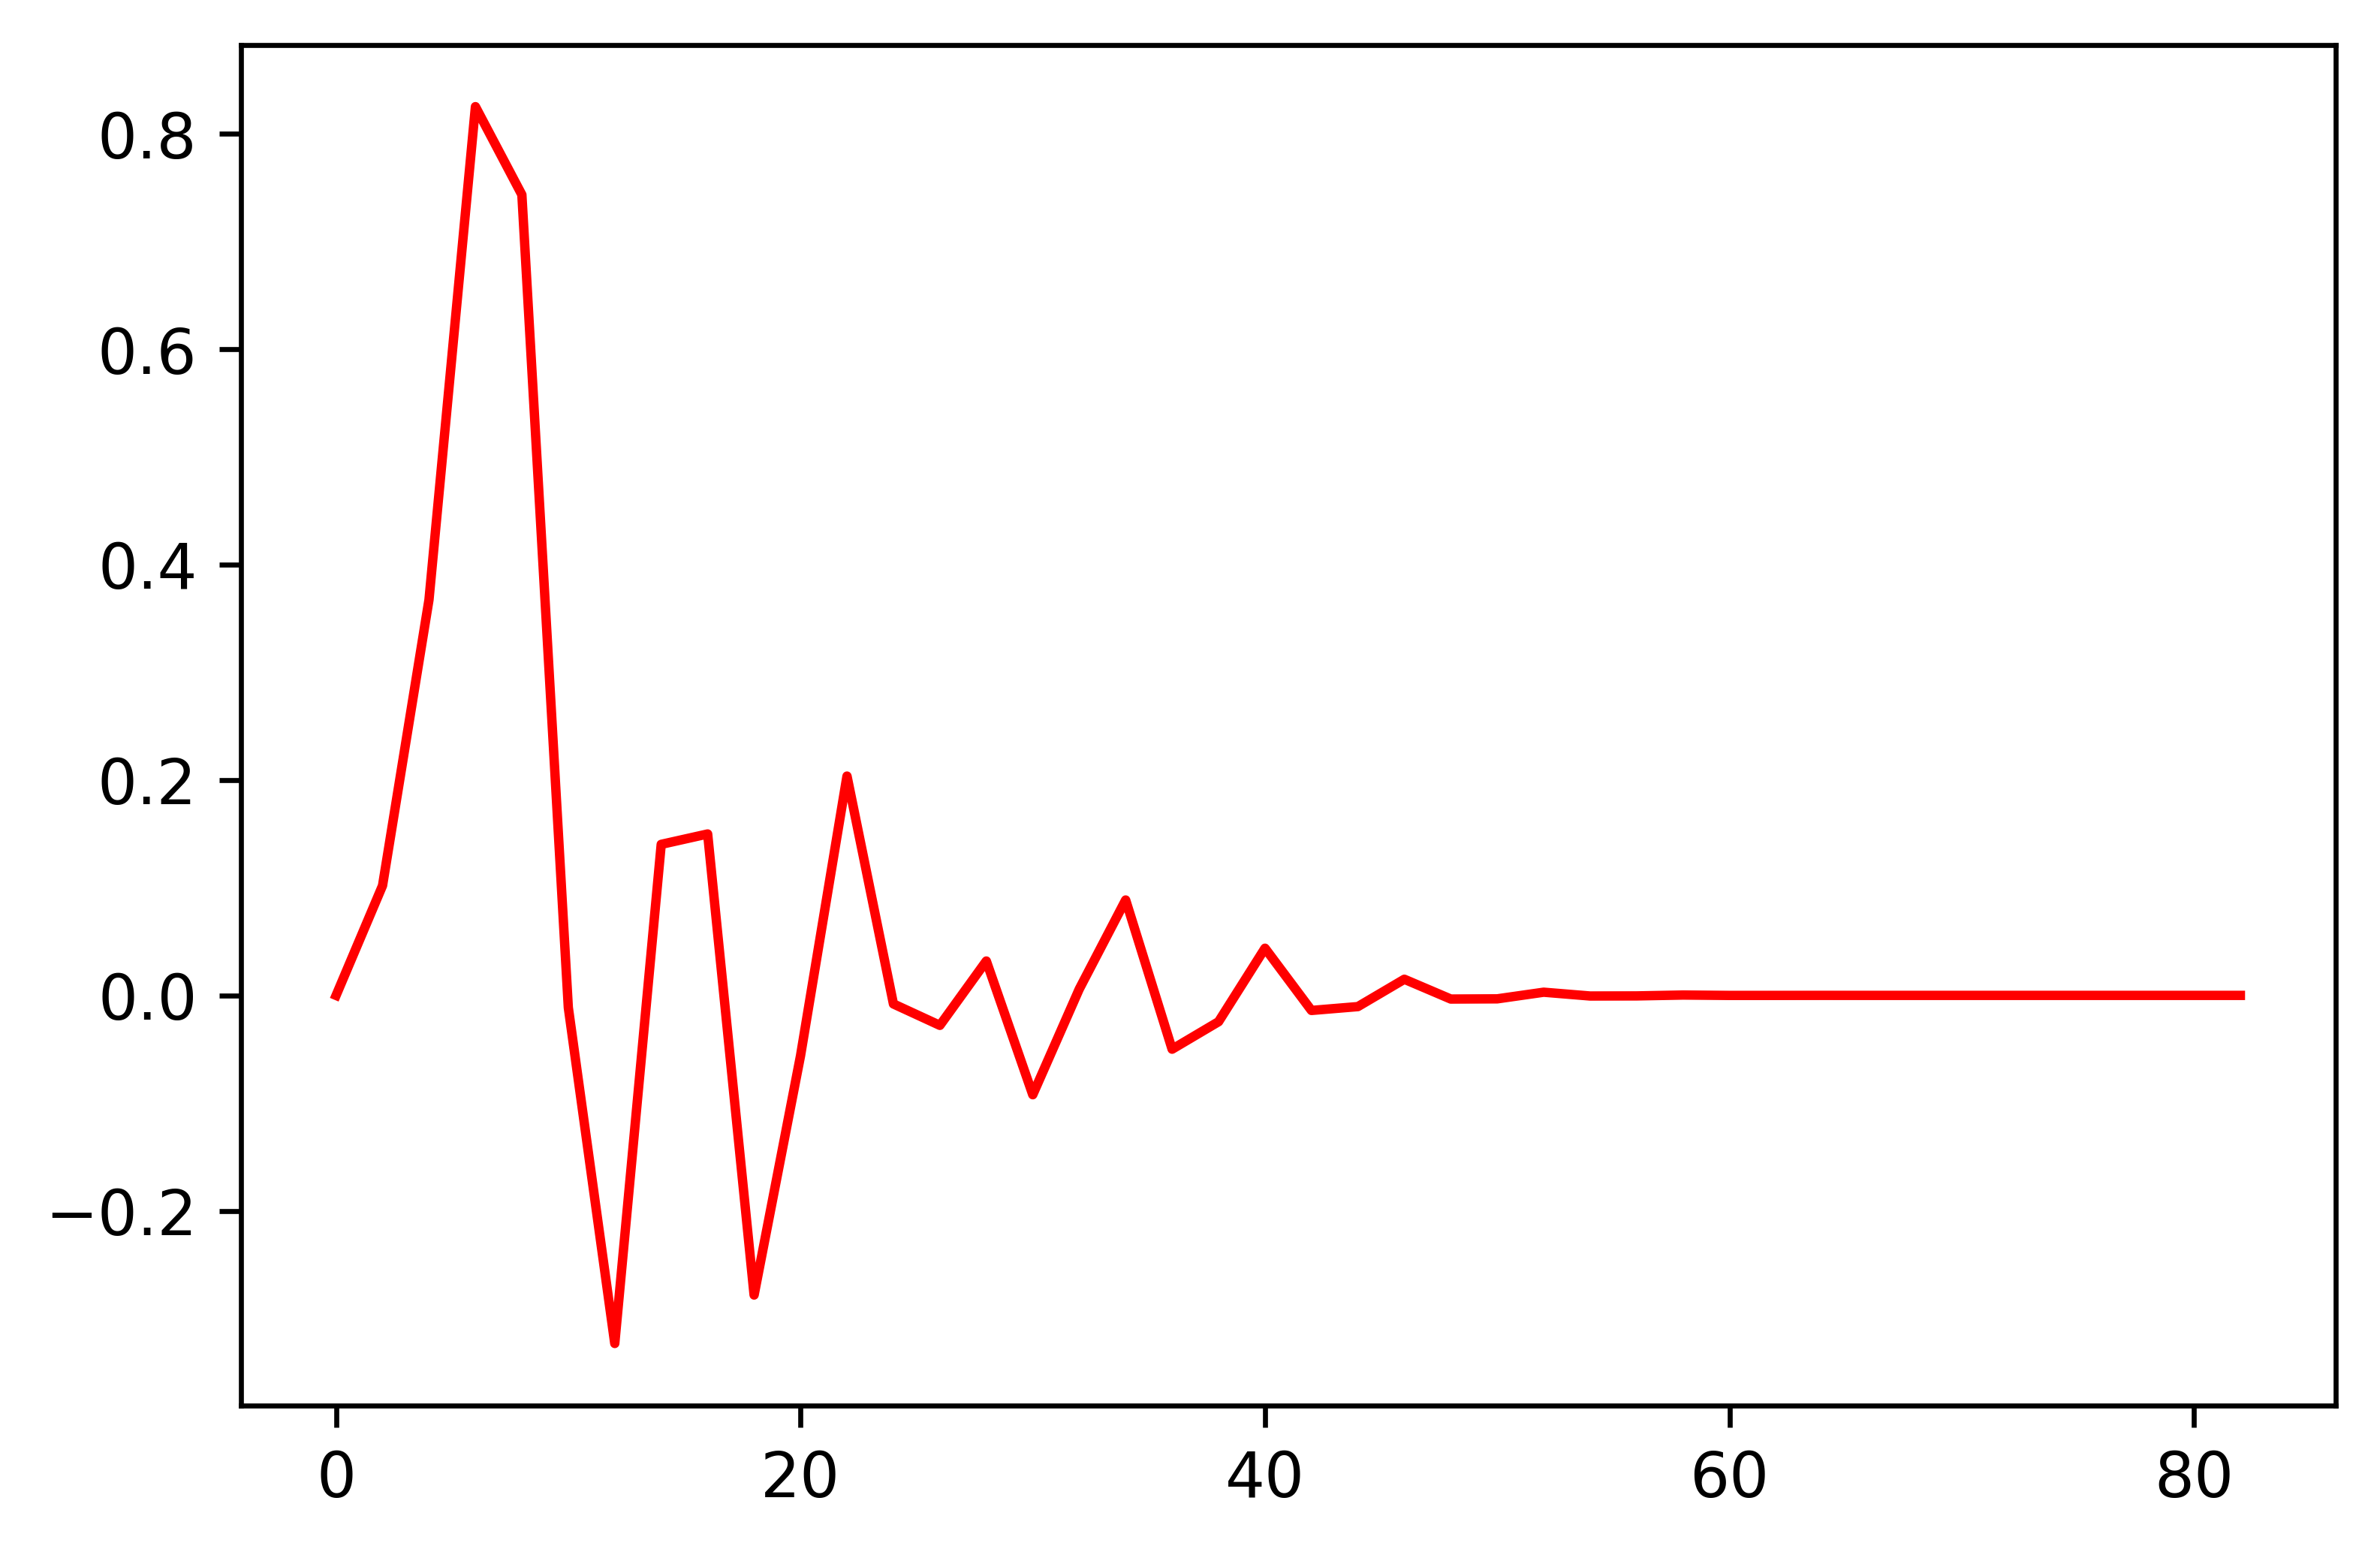
\includegraphics[scale=0.5]{Graphics/failed-example-red-shapelet.png}}
	\subfigure[DST-II y medida $\mathbb{S}$]{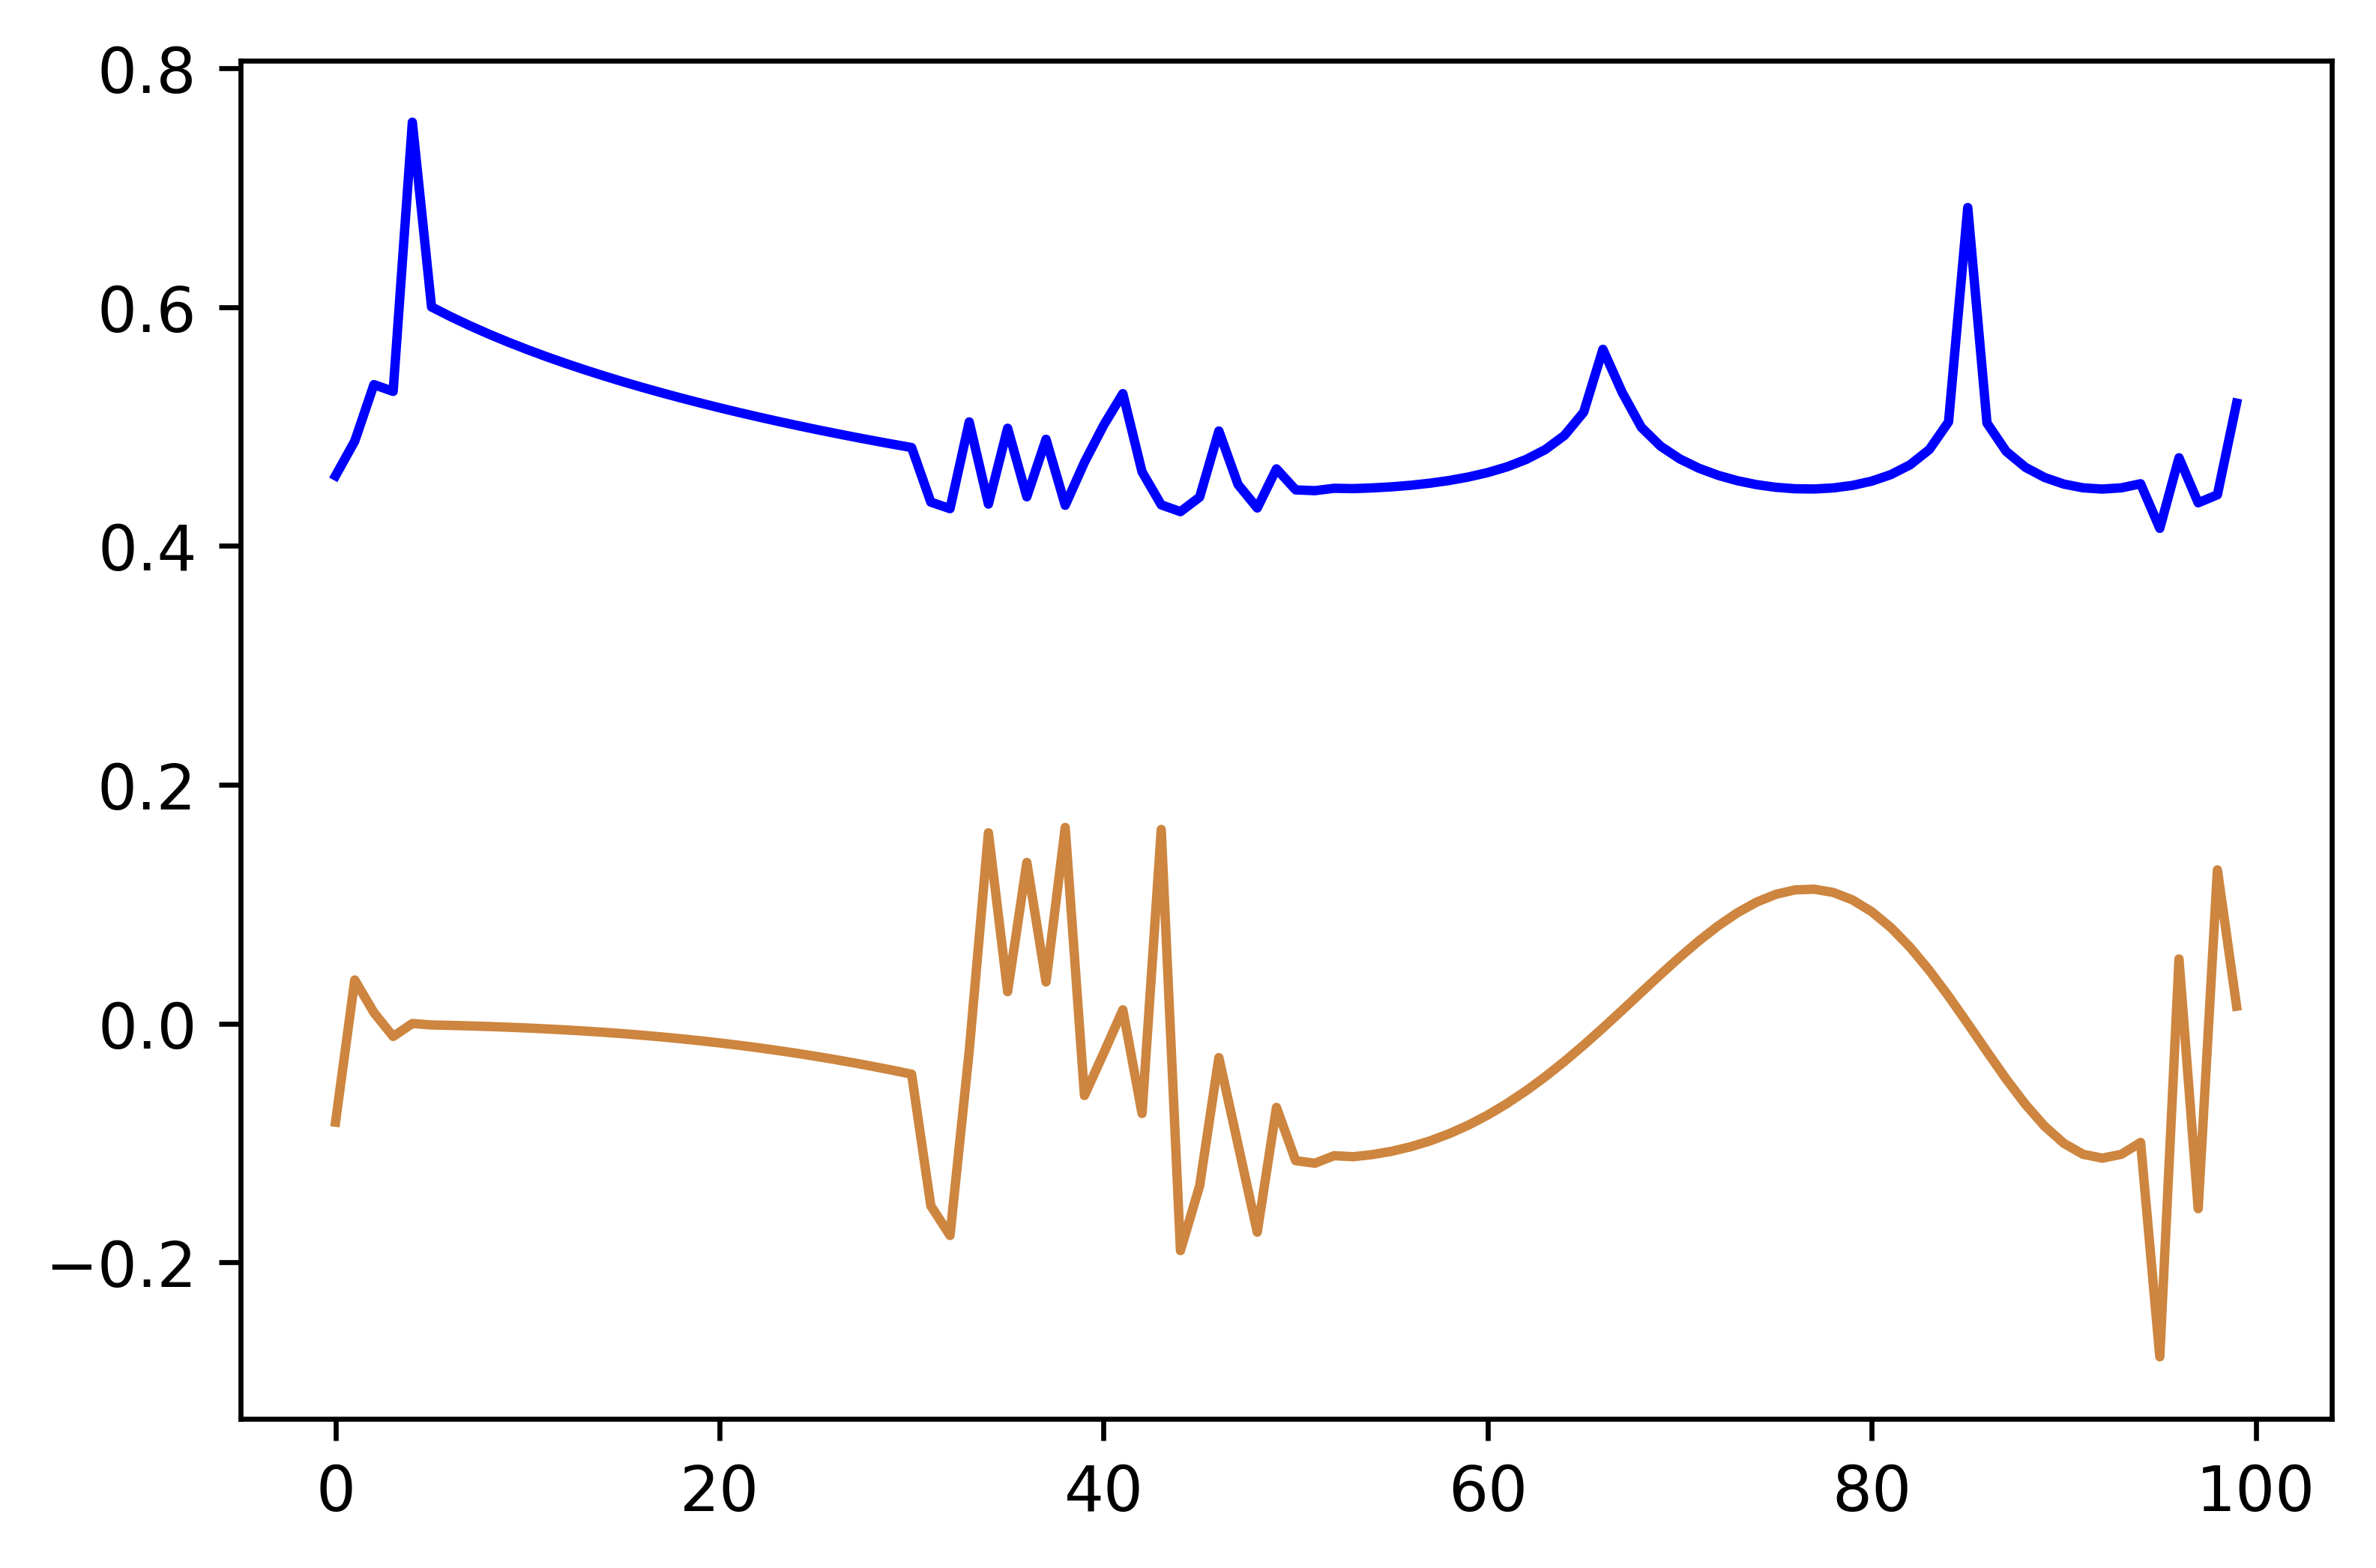
\includegraphics[scale=0.5]{Graphics/failed-example-detection.png}}
	\caption{Ejemplo donde el algoritmo no logra detectar la posición donde se encuentra el patrón.} \label{fig:failed-example-experiment}
\end{figure}

\section{Detección de patrones en señales 2D}

Una vez evaluada la capacidad de detección de la DST-II, se procede a la exploración de sus capacidades 
para el caso de señales 2D. A continuación se describen los experimentos y resultados.

Para llevar a cabo la experimentación se crearon imágenes artificiales con figuras simples. Entre ellas se incluyen gaussianas,
círculos y zonas rectangulares. El objetivo es evaluar la capacidad del algoritmo para detectar en el caso de 2D
y su sensibilidad ante el ruido. Sobre cada una de estas figuras se utilizó cada una de las propuestas realizadas 
en la Sección \ref{section:2d}.
El resultado se evaluaba visualmente, sobre el  mapa de colores (Figura \ref{fig:colormap}) donde las tonalidades azules representan
valores cercanos a 0 y las amarillas cercanas a 1.

\begin{figure}
	\centering
	
\includegraphics[scale=0.8]{Graphics/colormap.png} 
	\caption{Mapa de colores usado para evaluar la detección de la DST-II. Valores pequeños son representados en tonalidades azules y valores altos en amarillo.} \label{fig:colormap}
\end{figure}

\subsection{Ejemplos de los experimentos y análisis de los resultados}

\begin{figure}
	\centering
	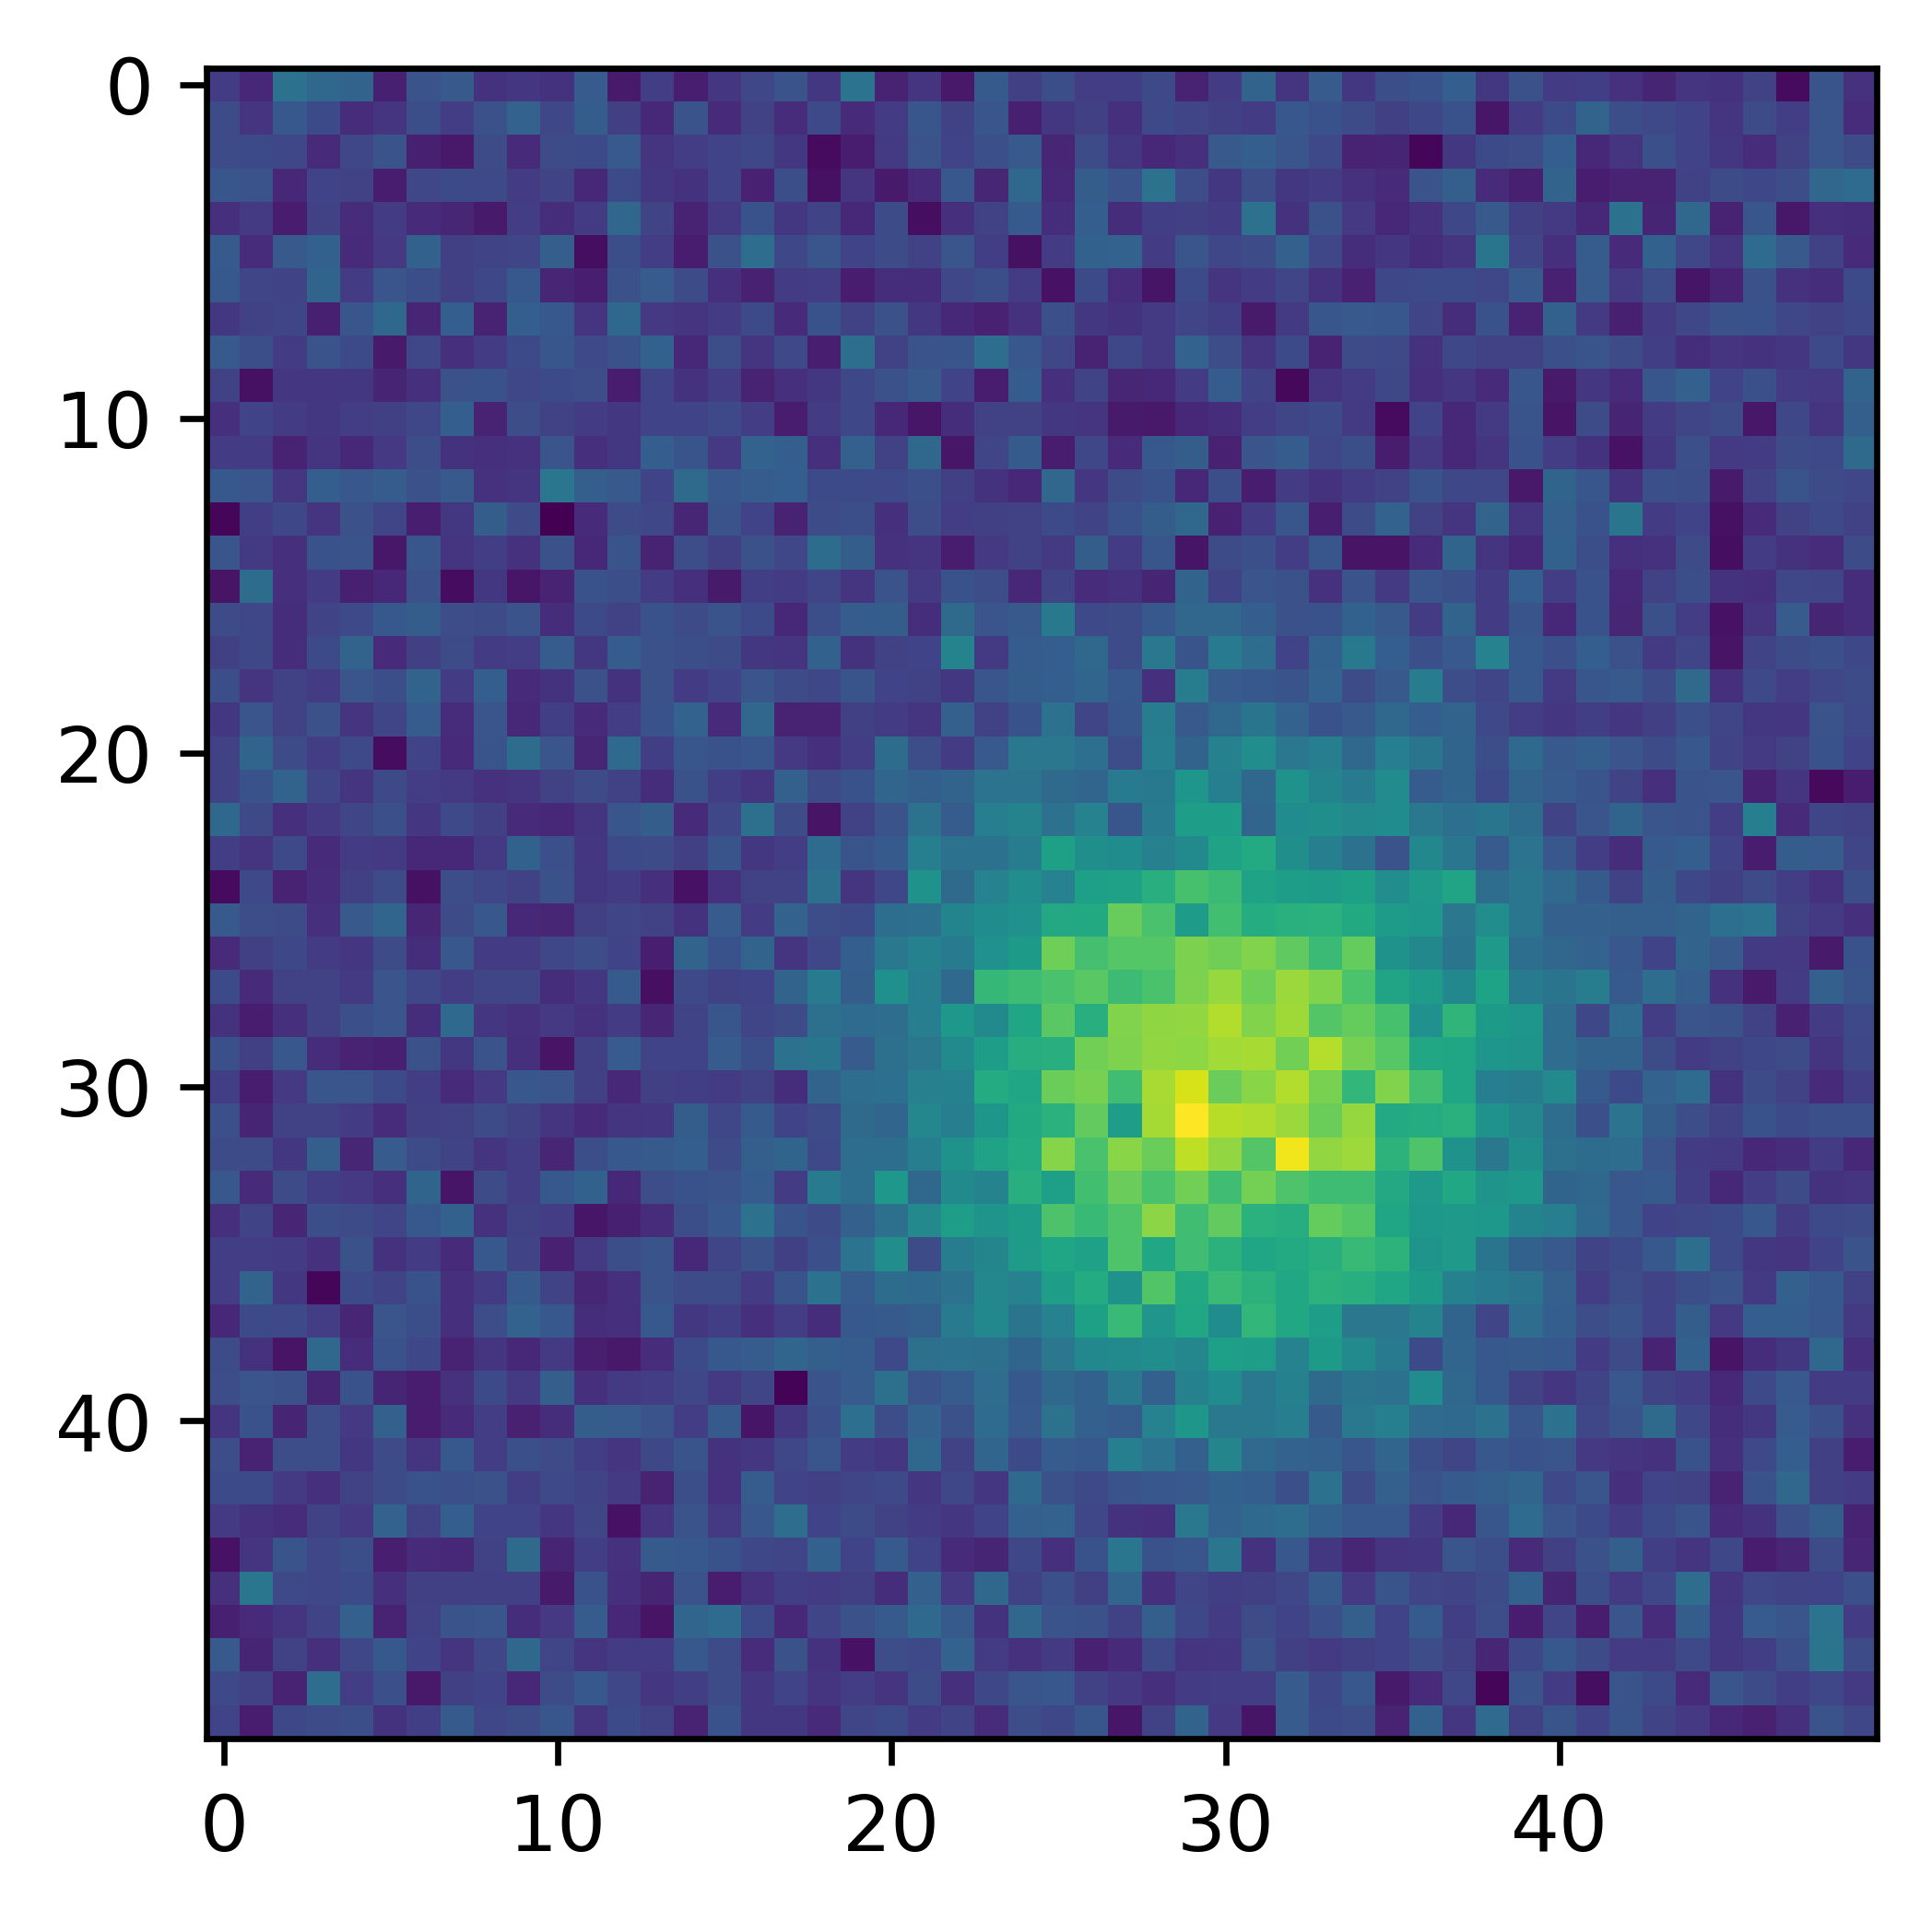
\includegraphics{Graphics/gaussian-2d-experiment.png}
	\caption{Gaussiana centrada en la posición (30,30).} \label{fig:gaussian-example-experiment}
\end{figure}

\begin{figure}
	\centering
	\subfigure[Sección horizontal]{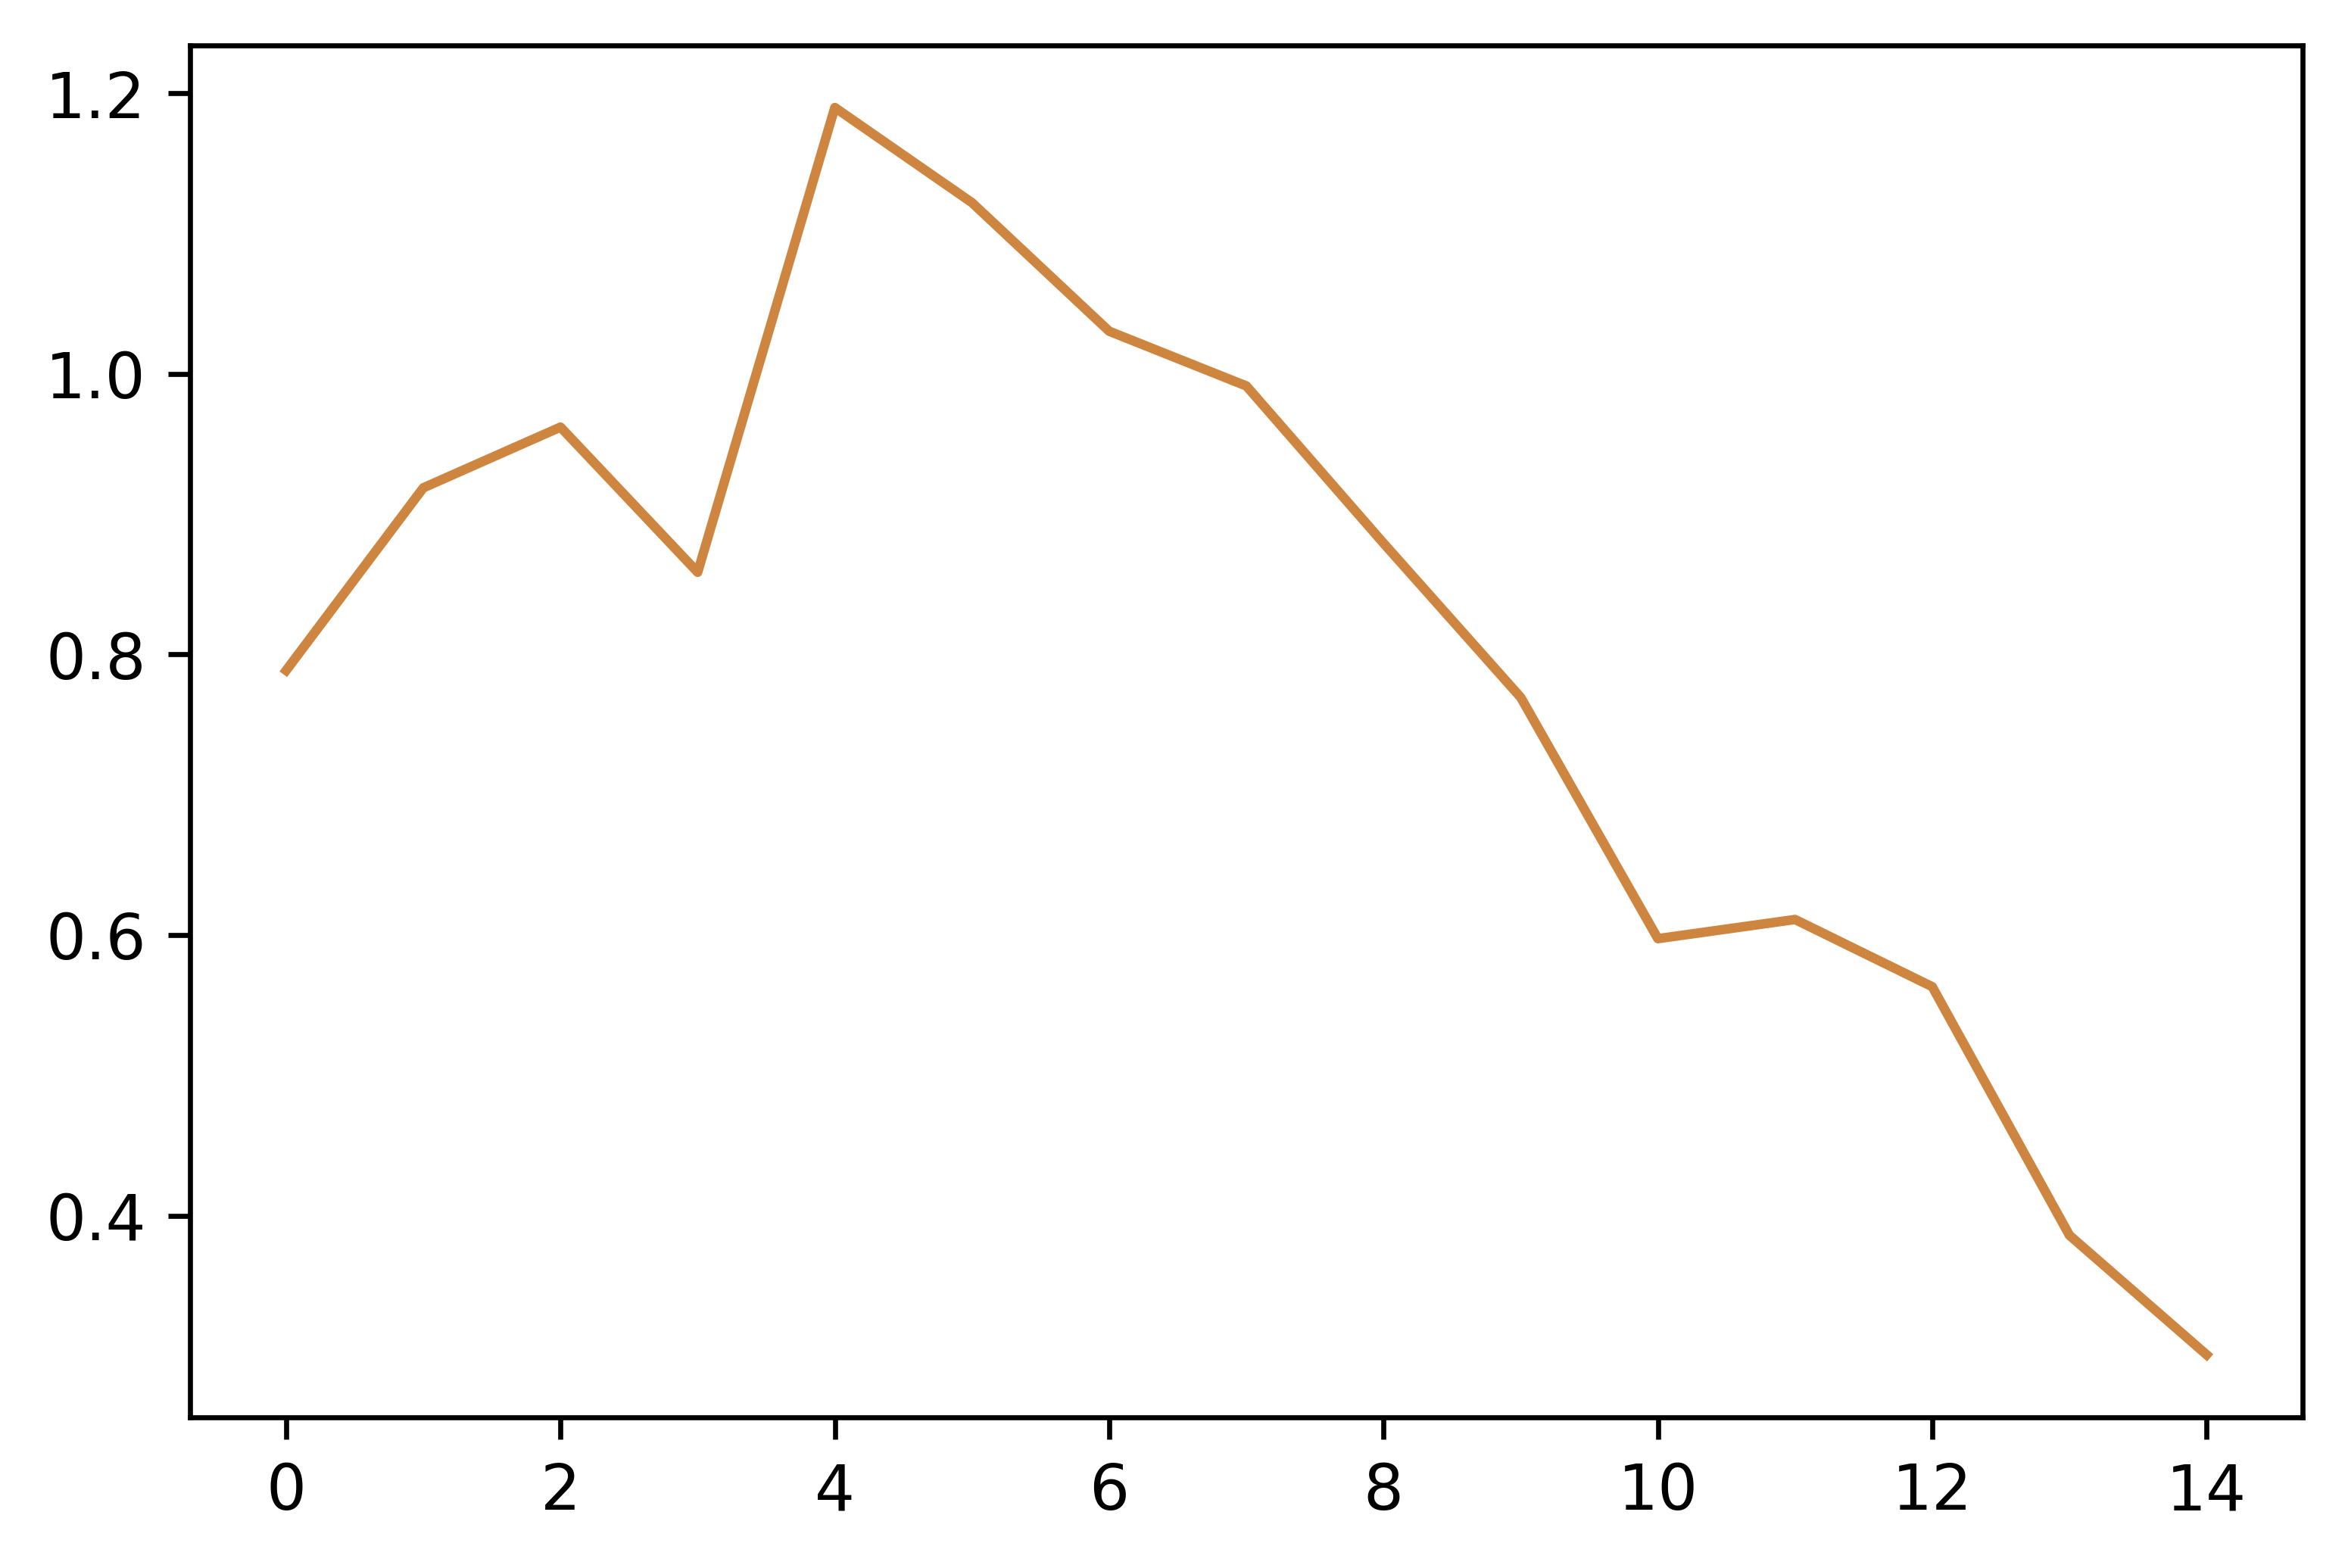
\includegraphics[scale=0.5]{Graphics/line-gaussian-experiment.png}}
	\subfigure[Sección vertical]{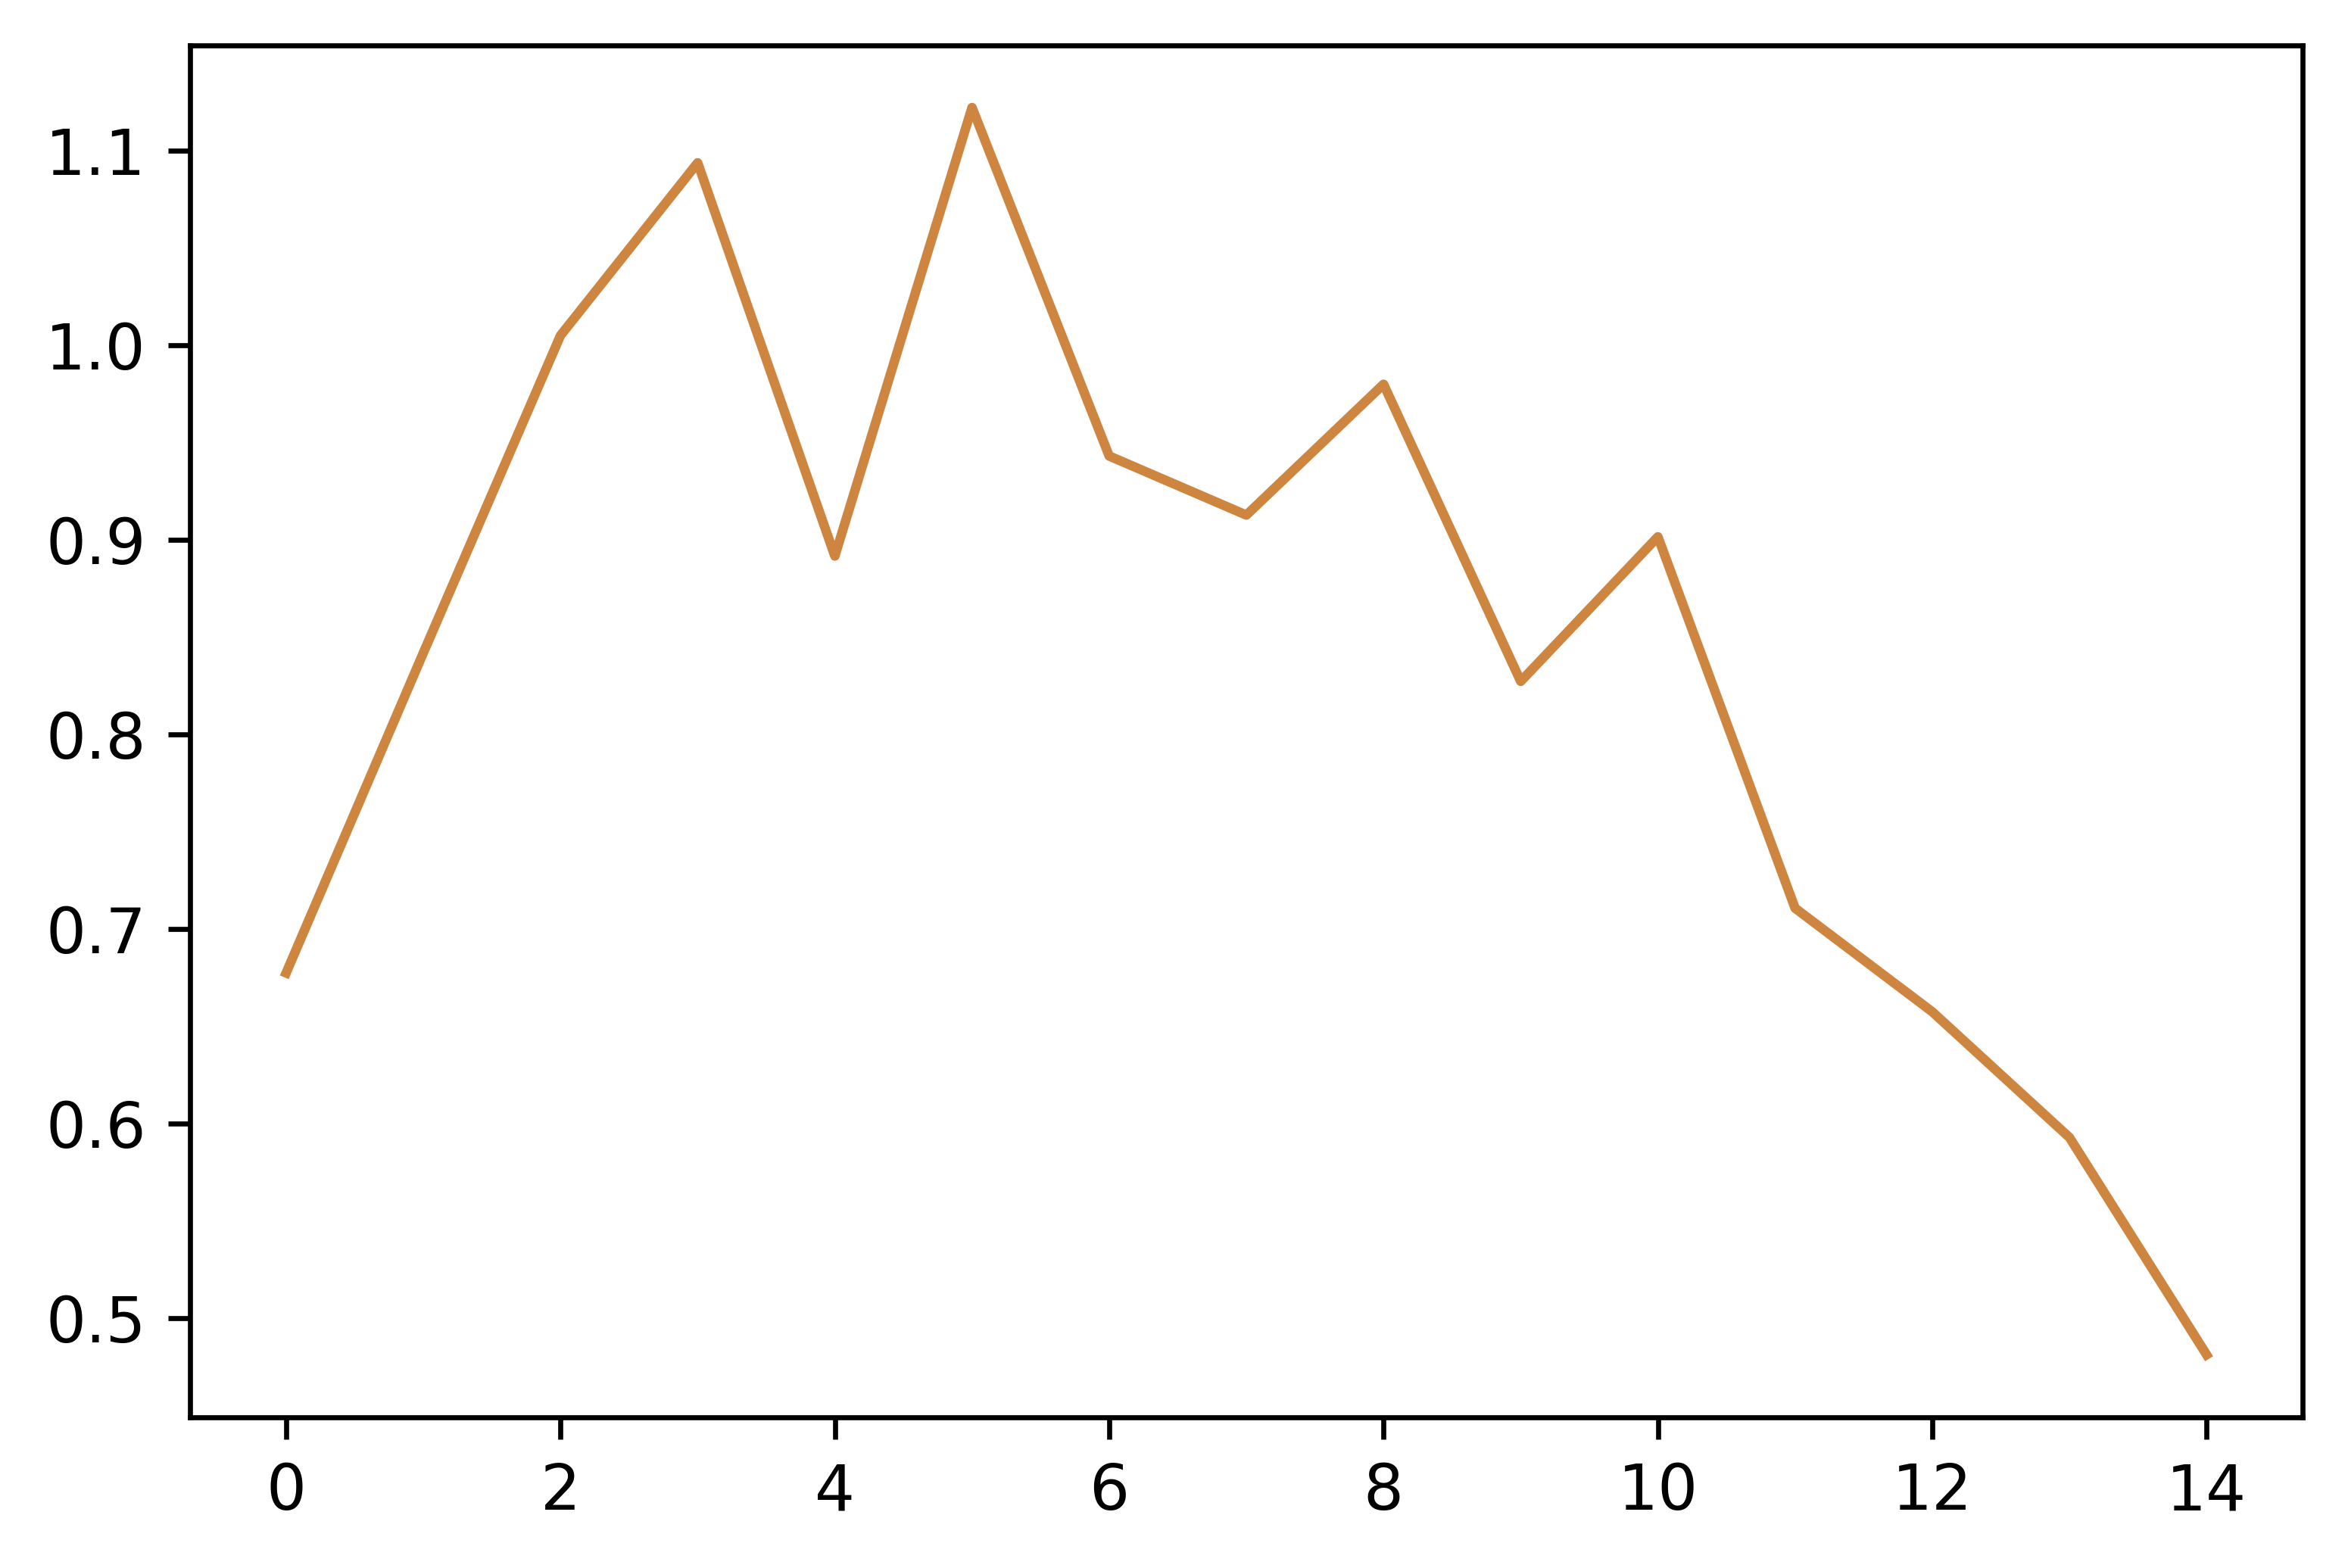
\includegraphics[scale=0.5]{Graphics/line-gaussian-experiment-vertical.png}}
	\caption{ Secciones correspondientes a [30,25:40] y [25:40,30] de la Figura \ref{fig:gaussian-example-experiment}.} \label{fig:lines-experiment}
\end{figure}

Como ejemplo se toma la imagen de la Figura \ref{fig:gaussian-example-experiment}. Siguiendo el primer enfoque,
se toman las secciones mostradas en la Figura
\ref{fig:lines-experiment} y se construyen dos \textit{shapelets} (una para las columnas y otra para las filas), obteniéndose cuatro componentes
al realizar la transformada. La Figura \ref{fig:gaussian-example-approach1} muestra el resultado. Como se puede apreciar, en ninguno de 
los coeficientes se obtiene un contraste alto con el resto, y de hecho ninguno supera el valor de $\mathbb{S}(c)=0.8$.

Esto se debe a que las ecuaciones de detección están 
construidas para que la convolución entre la sección de la señal que se parece al patrón y 
el filtro, sea lo más cercano a cero en el coeficiente que corresponde a la posición donde está el patrón.
Sin embargo, como se explica en el epígrage \ref{section:dwt-2d}, primero se realiza la transformada sobre las filas y 
luego al resultado
se le realiza nuevamente la transformada, pero en las columnas. 

En el caso de la primera transformada la detección es posible, y funciona de igual forma que si fuera una señal
unidimensional, solo que ahora se realiza por las filas. 
Pero, una vez que se pasa a la segunda transformada sobre las columnas, las condiciones para la detección del patrón no se cumplen.
Las ecuaciones (\ref{eq:matching-1}) (\ref{eq:matching-2}) están diseñadas para que la convolución sea lo más cercana 
a cero solamente si se está pasando el filtro sobre los valores del patrón, no sobre su transformada.

Esto limita la extensión de las capacidades de detección de la DST-II para señales de más de una dimensión, 
tal y como se puede
apreciar en el ejemplo anterior. Resultados similares se obtuvieron en otros ejemplos. Por lo tanto, esta no es una 
vía factible para extender la DST-II para señales bidimensionales.


\begin{figure*}
\begin{multicols}{2}
	\subfigure[Coeficientes de aproximación]{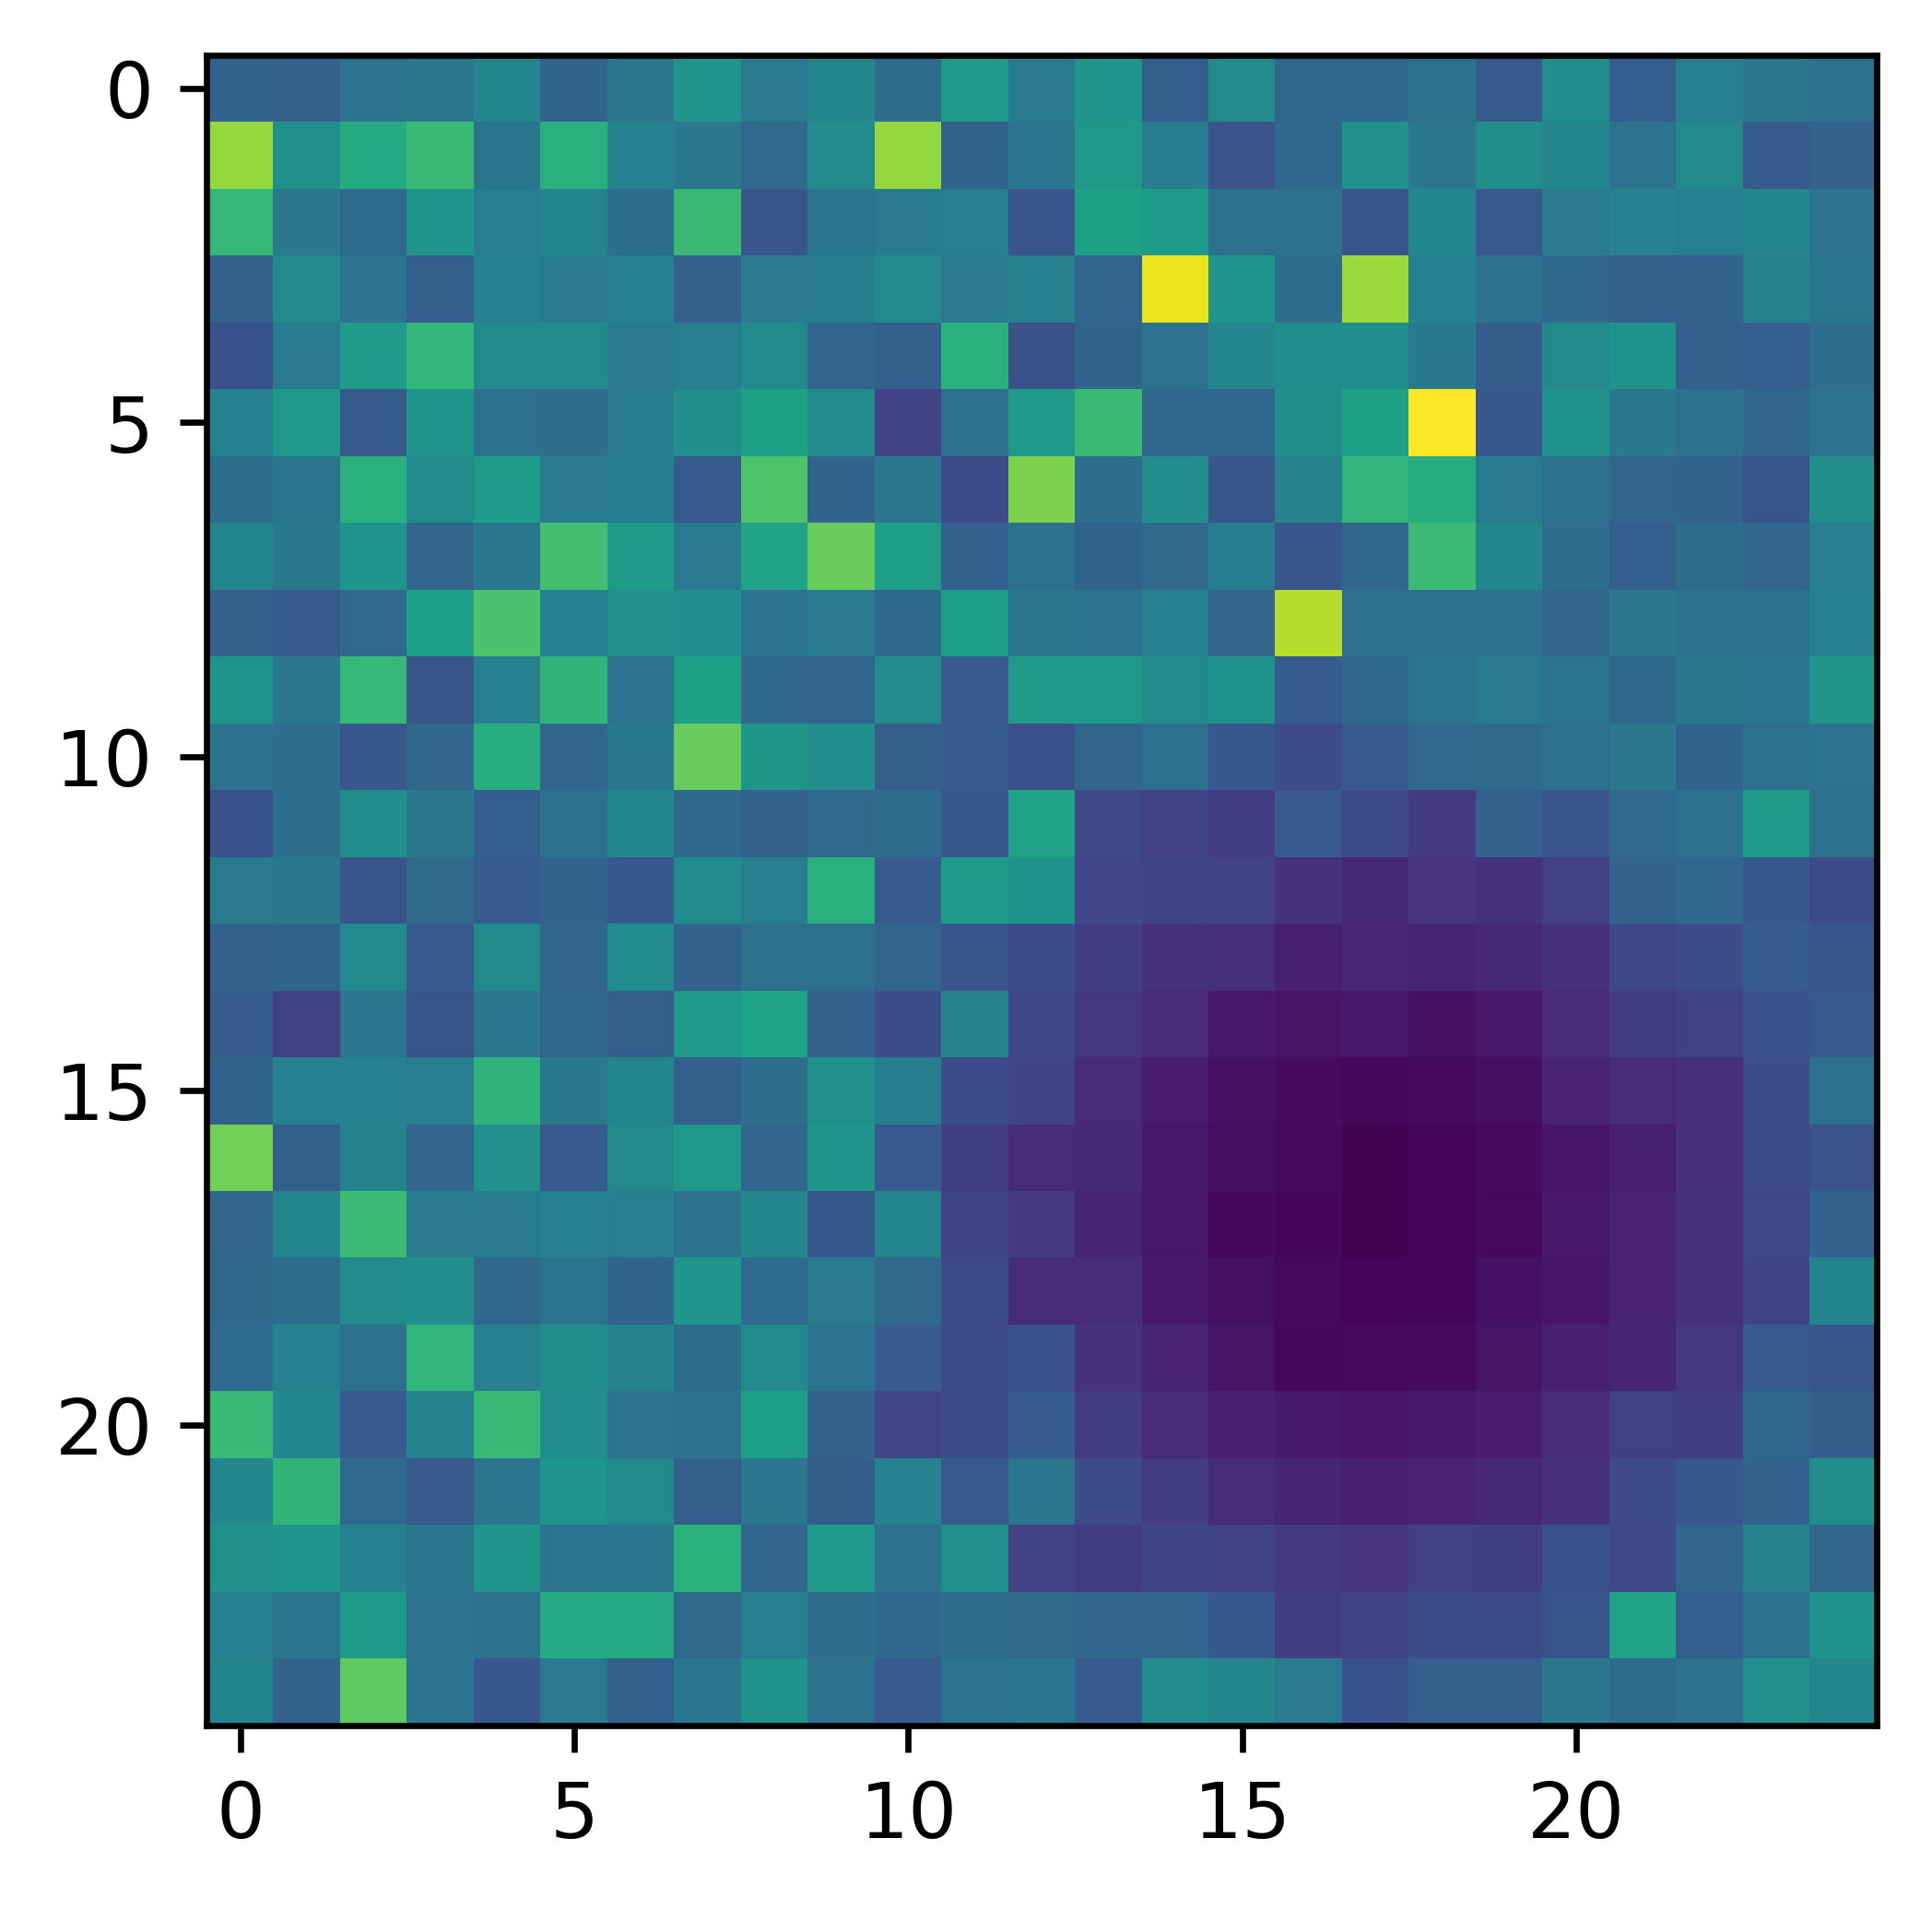
\includegraphics[width=\linewidth]{Graphics/guassian-2d-experiment-aprox.png}}\par 
	\subfigure[Coeficientes de detalle horizontal]{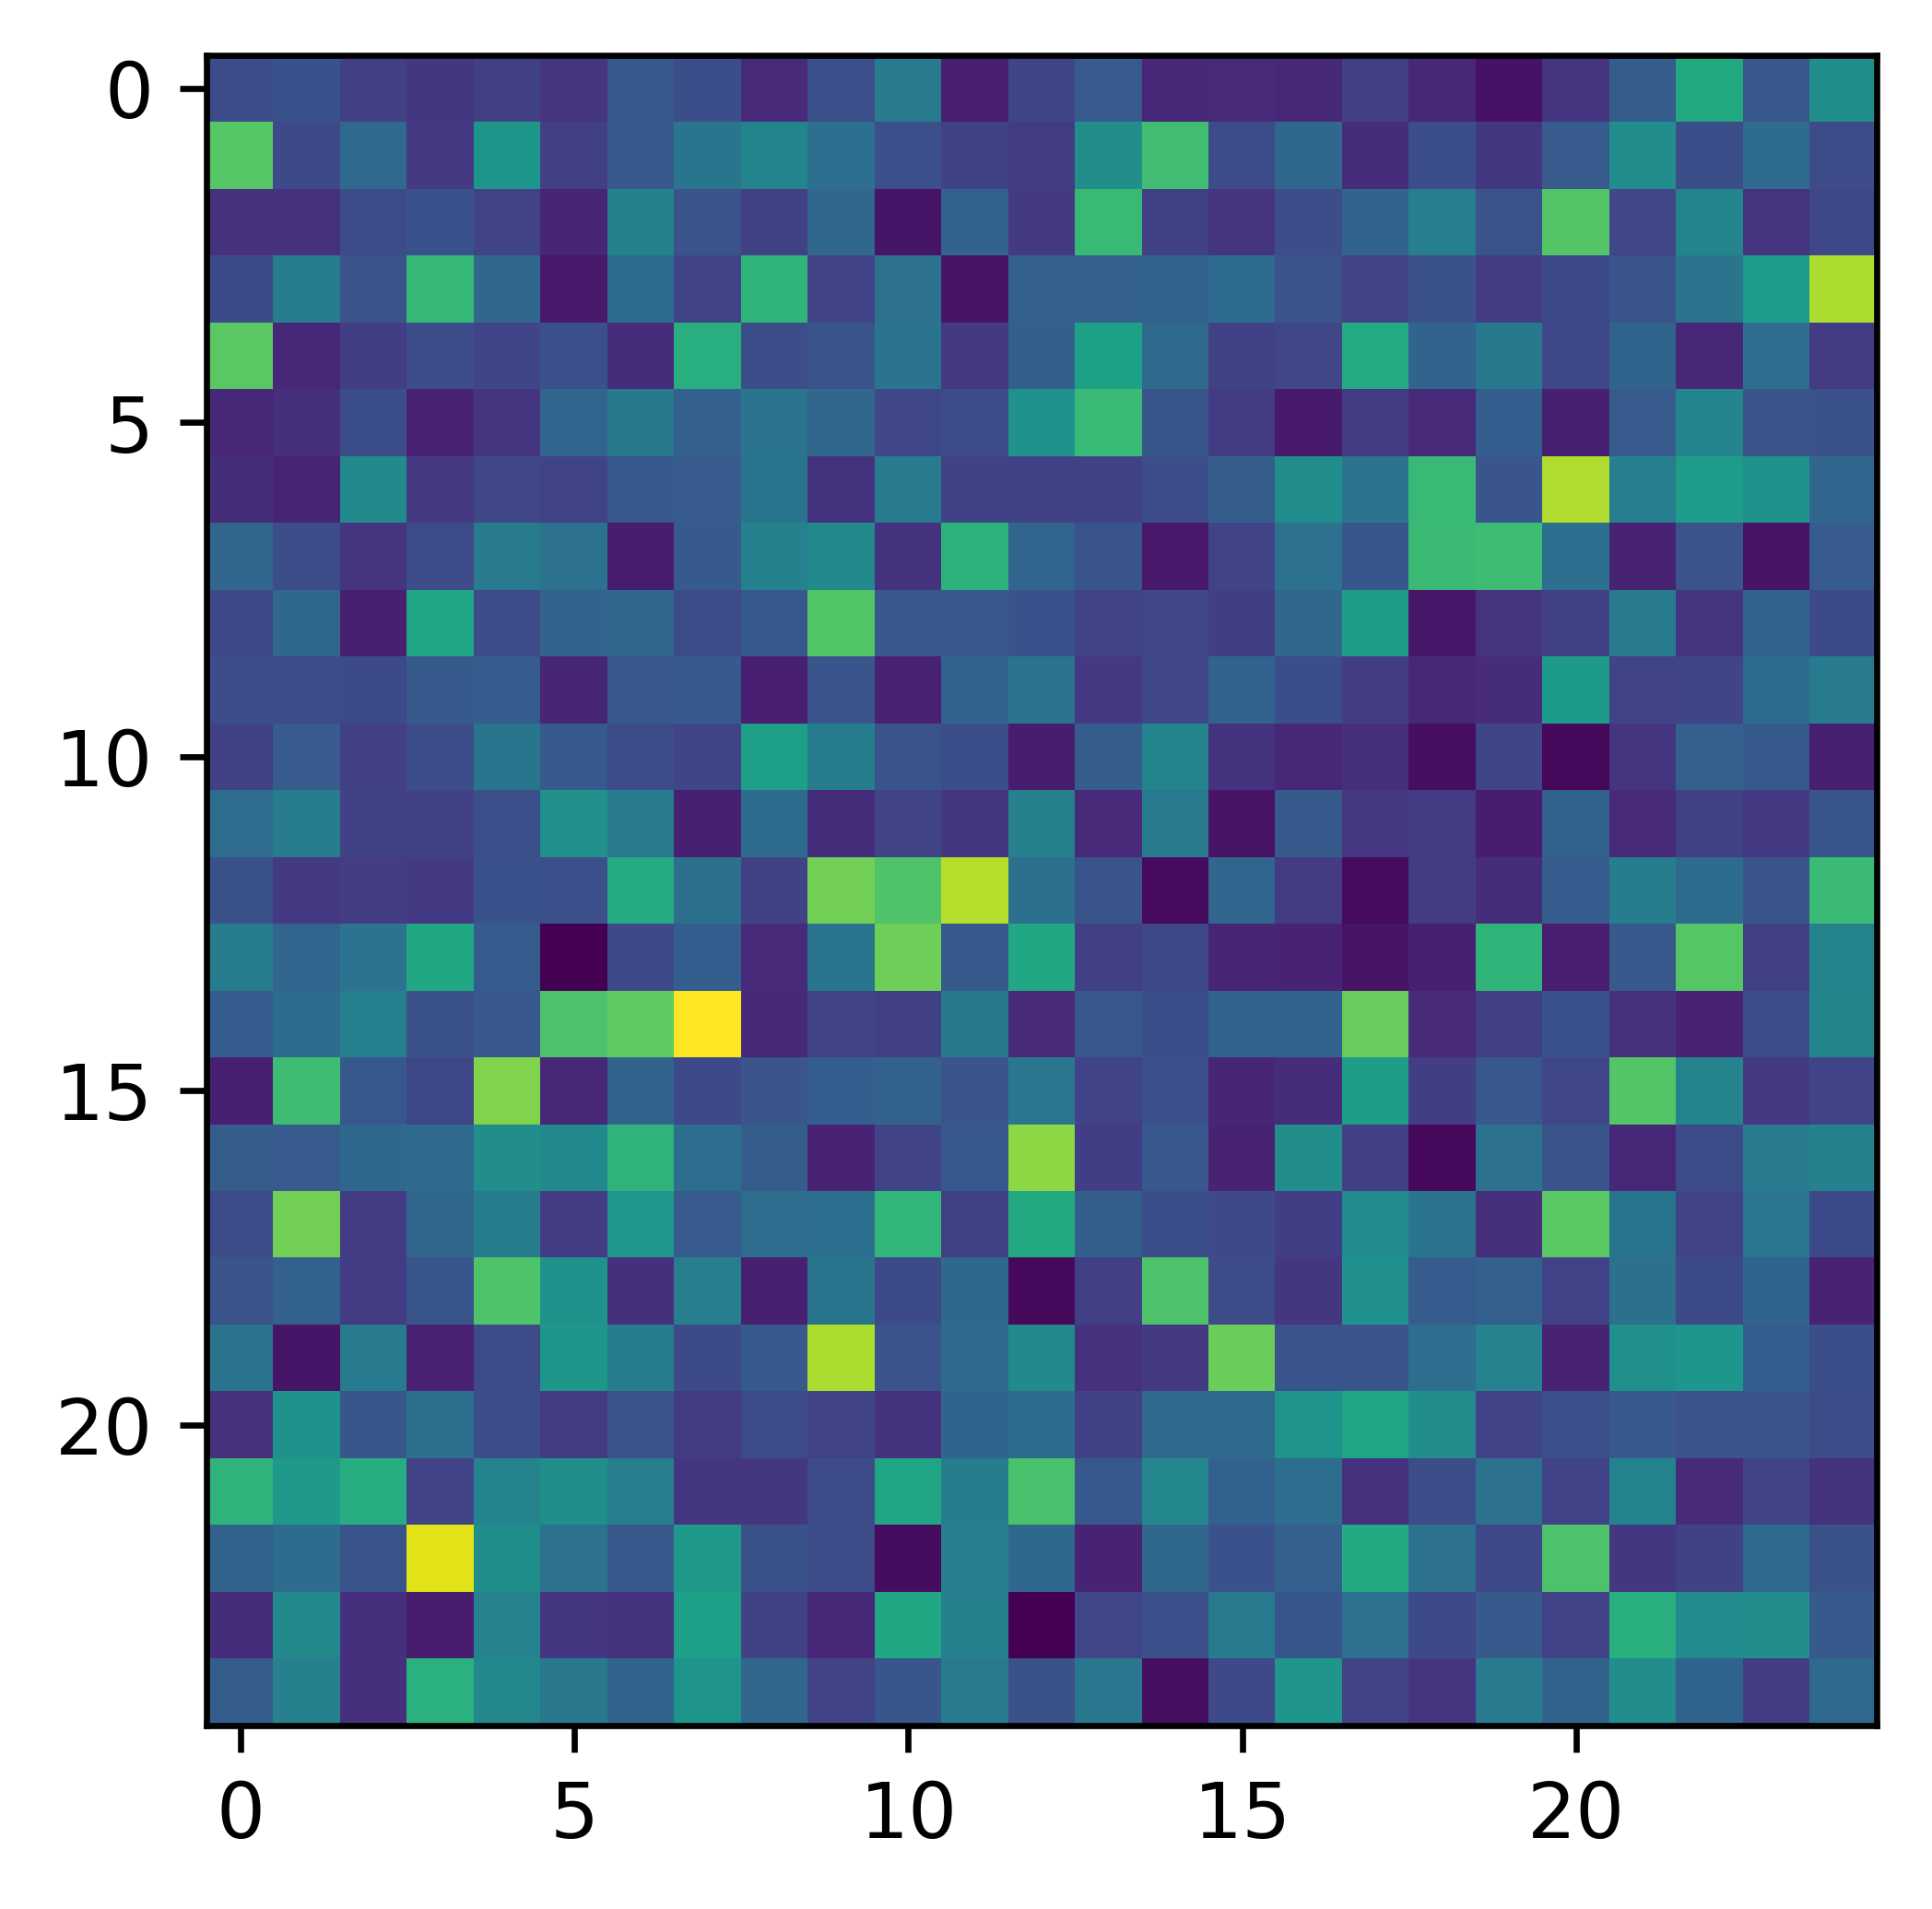
\includegraphics[width=\linewidth]{Graphics/gaussian-2d-experiment-horizontal.png}}\par 
    \end{multicols}
\begin{multicols}{2}
	\subfigure[Coeficientes de detalle vertical]{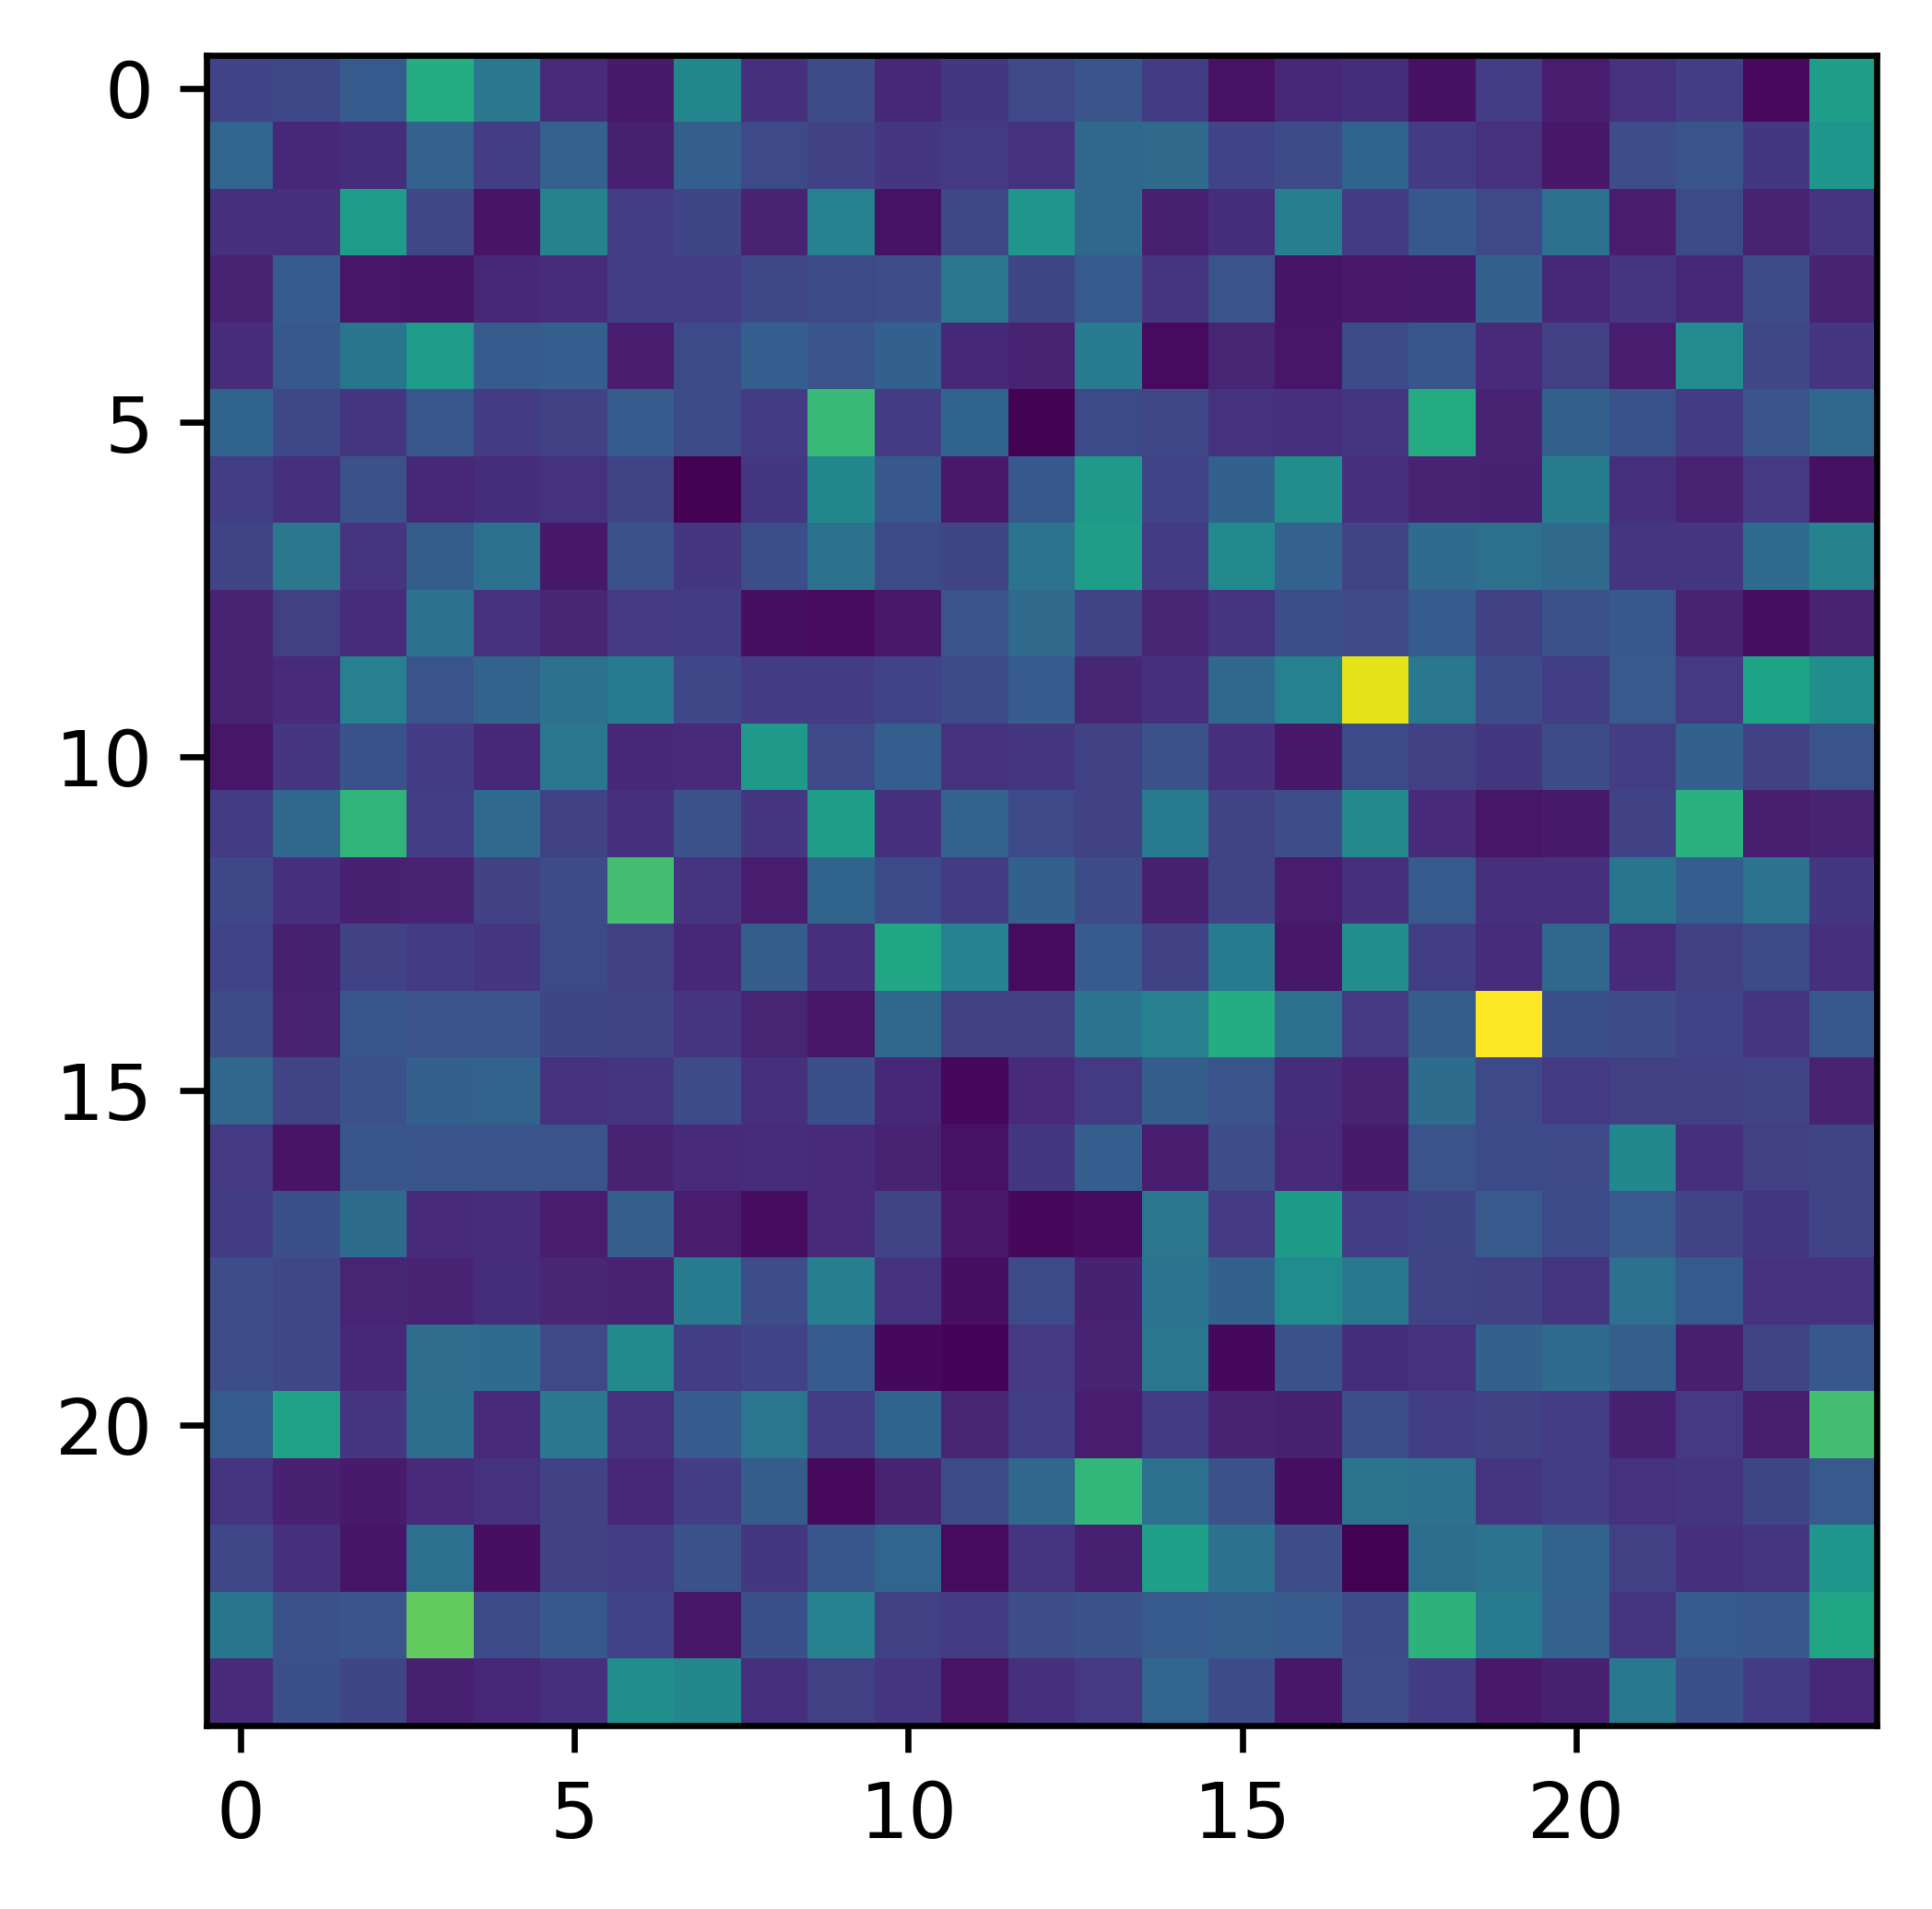
\includegraphics[width=\linewidth]{Graphics/gaussian-2d-experiment-vertical.png}}\par
	\subfigure[Coeficientes de detalle diagonal]{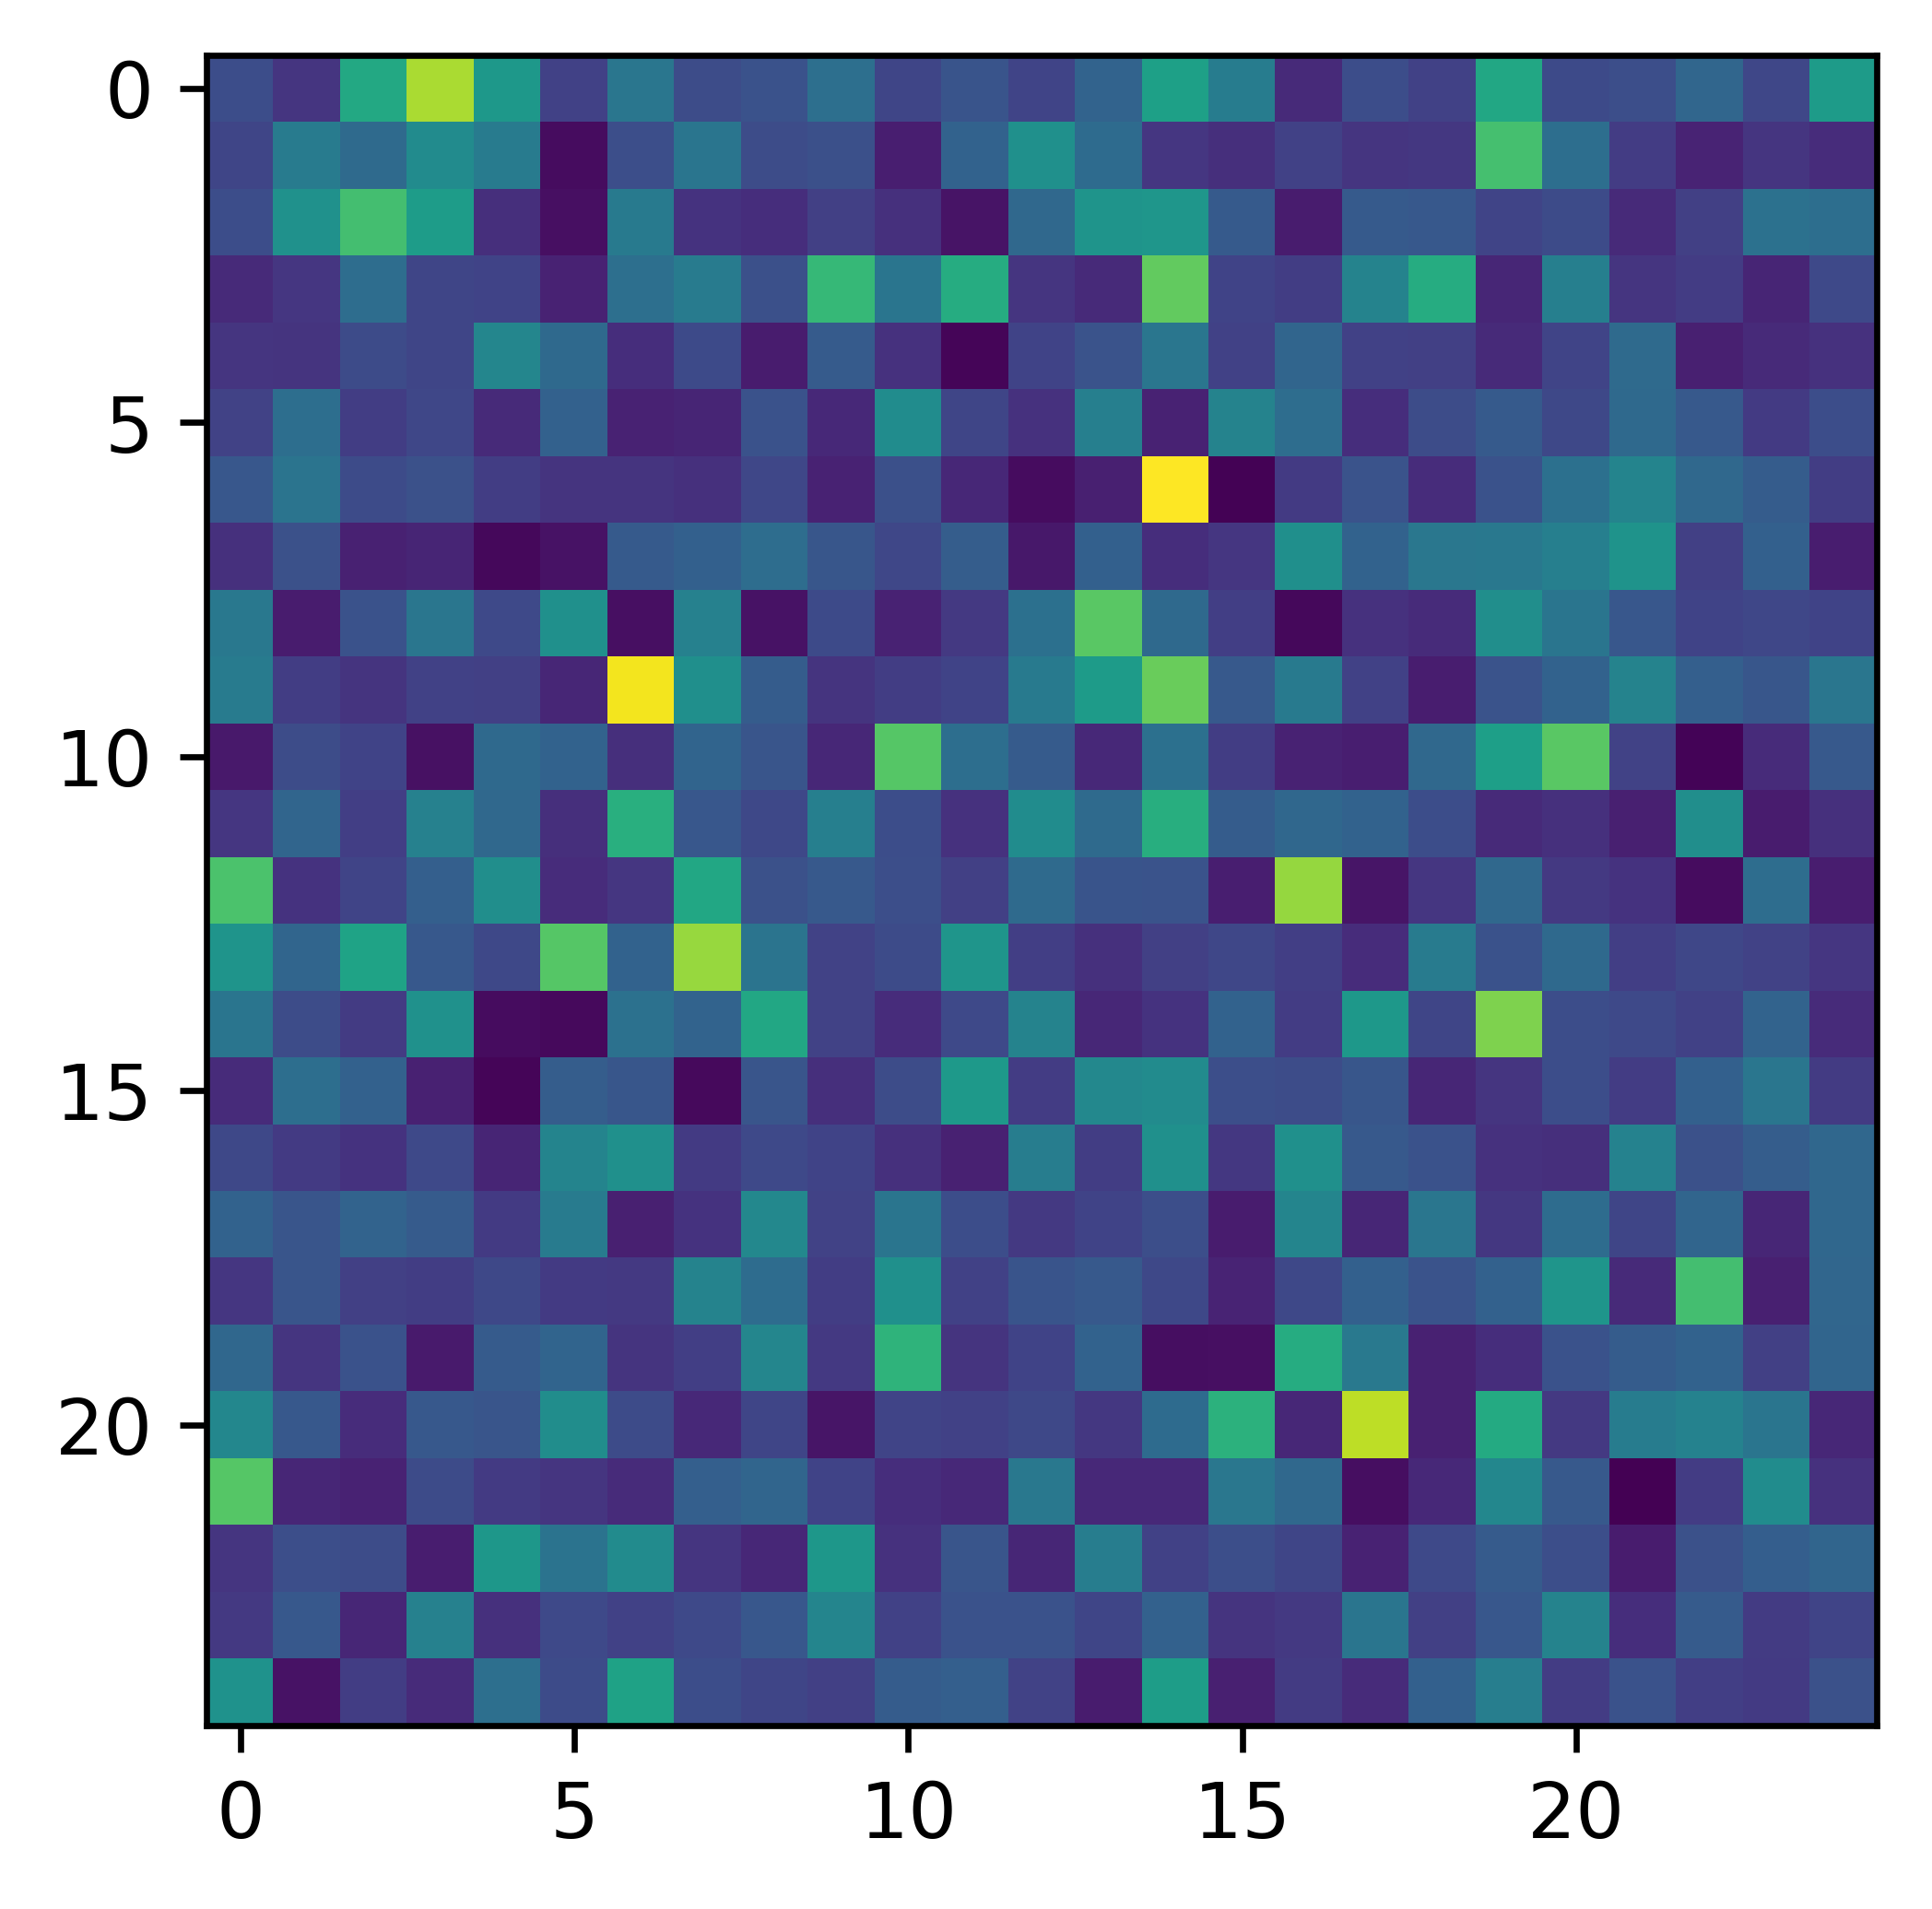
\includegraphics[width=\linewidth]{Graphics/gaussian-2d-experiment-diagonal.png}}\par
\end{multicols}
\caption{Resultado de evaluar $\mathbb{S}$ sobre cada uno de las componentes de la DST-II usando el primer enfoque.} \label{fig:gaussian-example-approach1}
\end{figure*}


El resultado del segundo enfoque se aprecia en la Figura \ref{fig:gaussian-example-approach2}.
En este caso sí se puede apreciar claramente que existe un coeficiente que sobresale
entre los demás al realizar la DST-II por filas. El mismo se encuentra en la posición $(30,16)$ con un valor de $\mathbb{S}=0.98$.
Esta posición corresponde aproximadamente al punto $(30,32)$ en la imagen original. Teniendo en cuenta que la
sección horizontal del patrón tomado está comprendida en el intervalo $[30,25:40]$, el resultado es bastante certero.

En el caso de la sección vertical, no se tuvo tanto éxito. No existe gran constraste entre ninguna posición con el resto. 
Esto se debe a que el error de las condiciones de detección es mucho mayor para la \textit{shapelet} de la sección
vertical que para la de la sección horizontal.

\begin{figure}
	\centering
	\subfigure[Por filas]{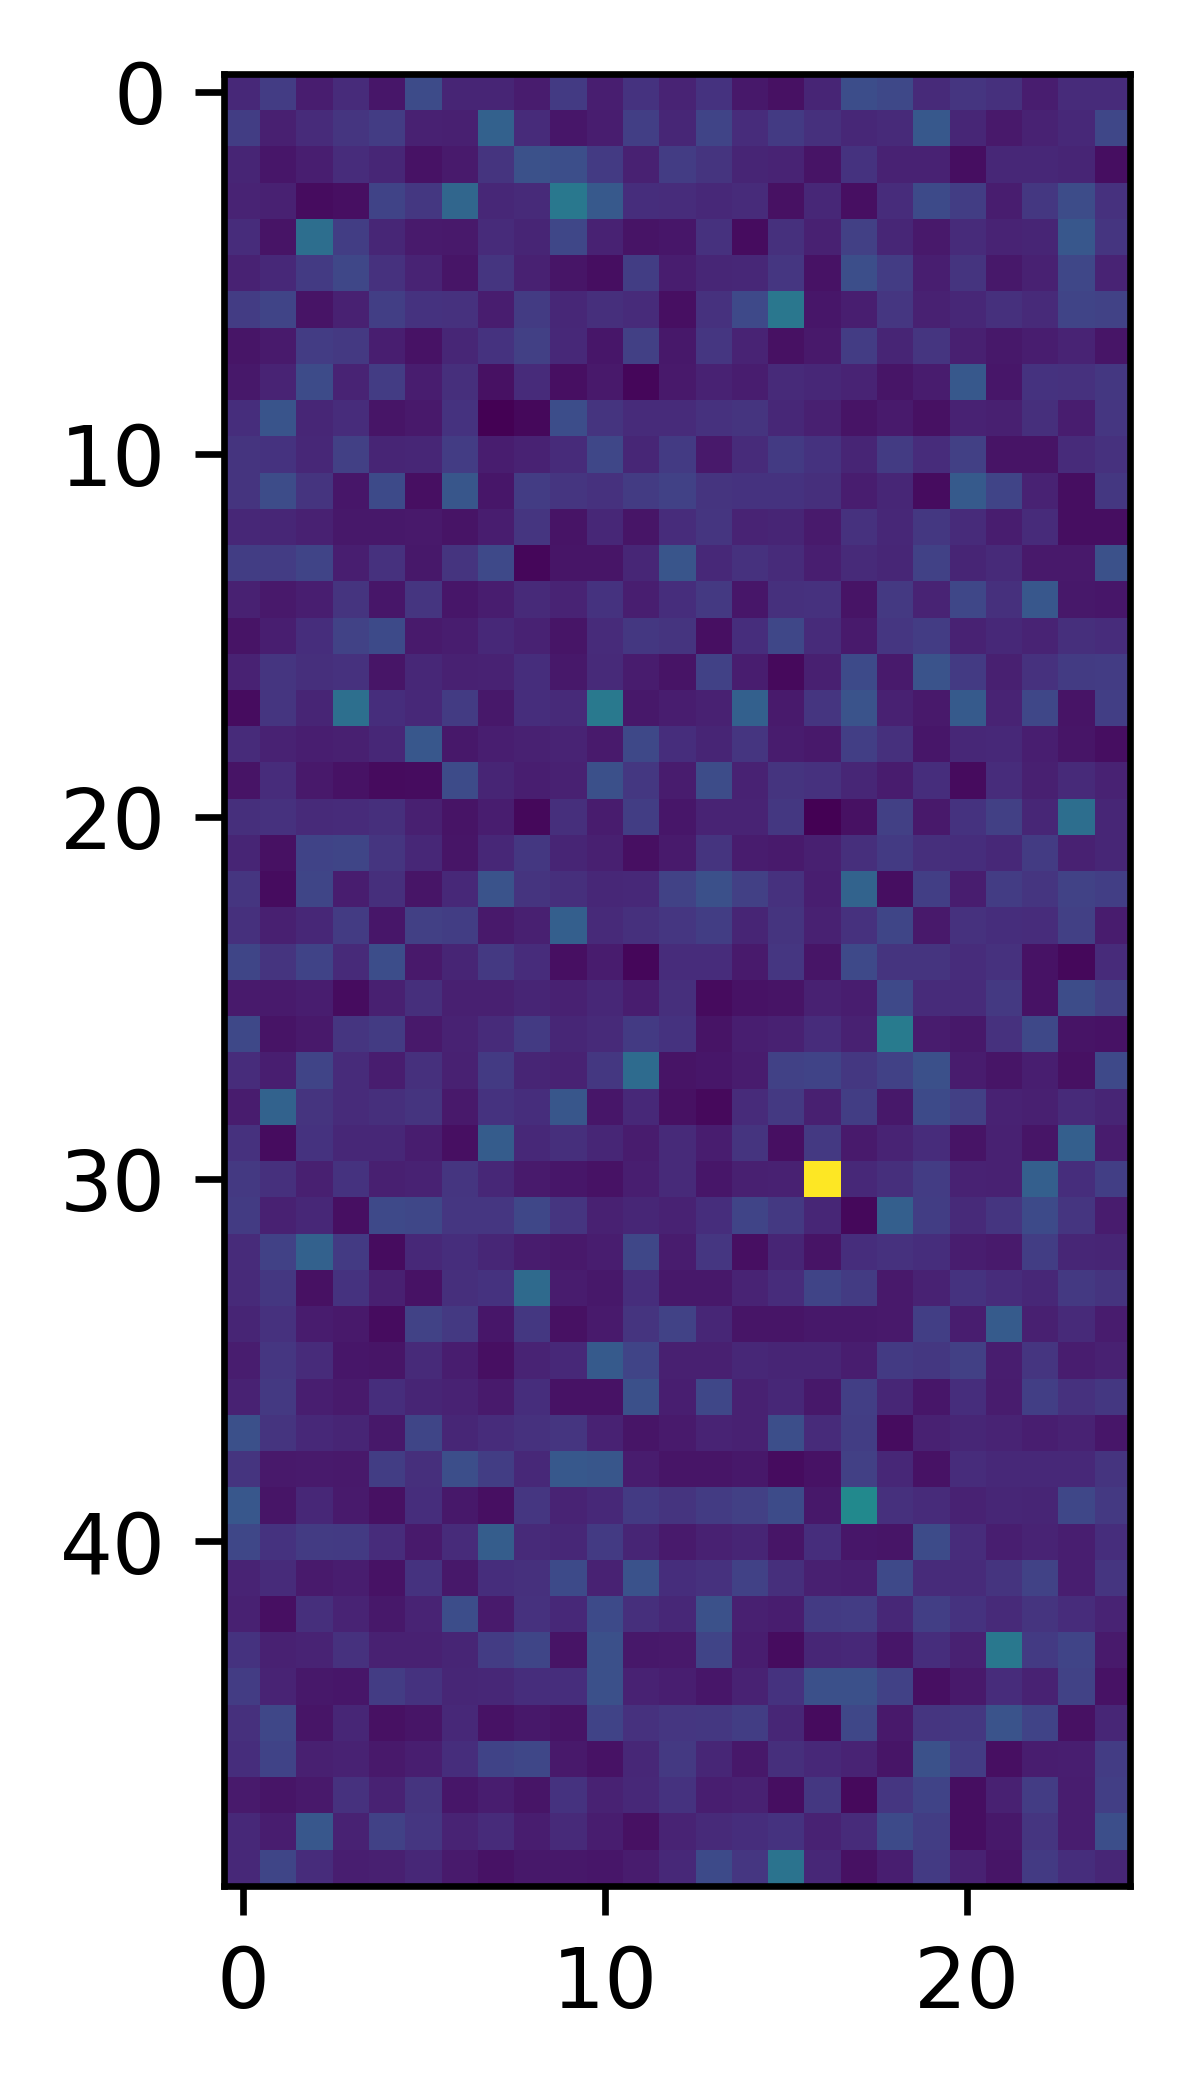
\includegraphics{Graphics/gaussian-2d-experiment2-row.png}}
	\subfigure[Por columnas]{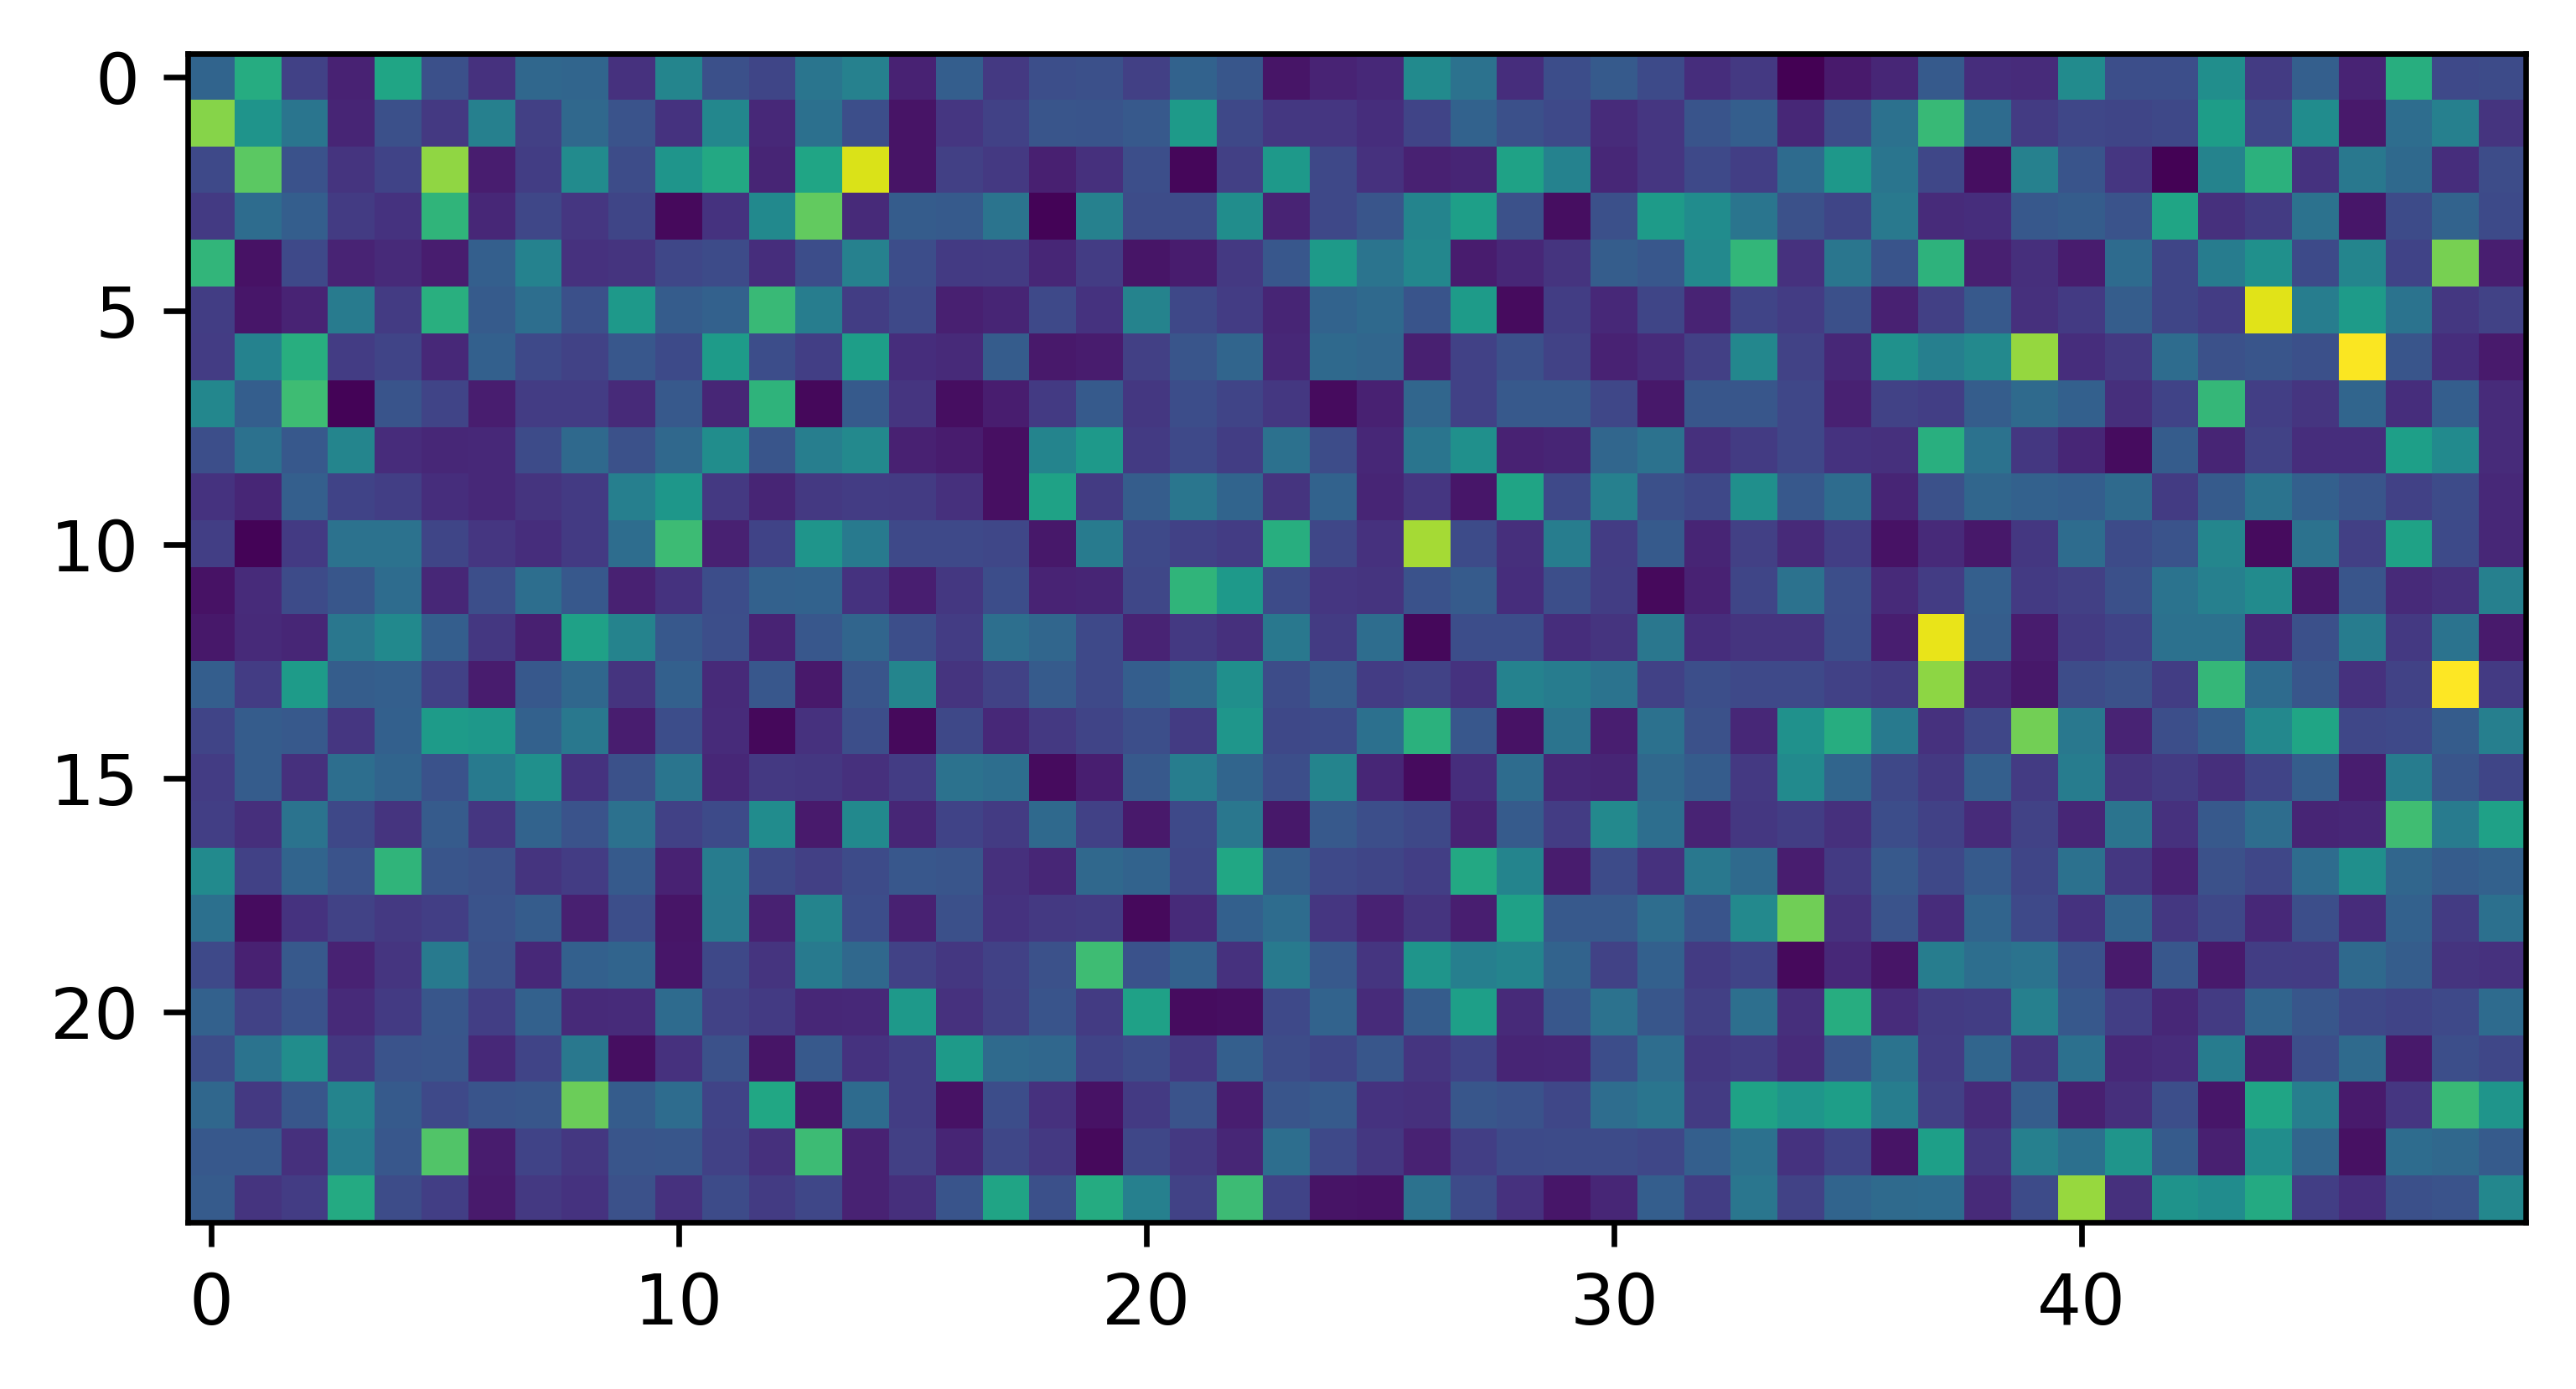
\includegraphics{Graphics/gaussian-2d-experiment2-col.png}}
	\caption{Resultado de evaluar $\mathbb{S}$ sobre cada una de las \textit{second-rated} de la DST-II usando el segundo enfoque.} \label{fig:gaussian-example-approach2}
\end{figure}
%-0.00781404414483181 col error matching
%0.0118491040034377
%-2.61711684291969e-18 row error matchine
%-8.05175395622083e-18

En el caso del tercer enfoque, se toma la región comprendida entre los píxeles $[25:40,25:40]$. Los resultados 
se muestran en la Figura \ref{fig:gaussian-example-approach3}. En este caso, se logra obtener toda una región con mayor 
contraste que corresponde aproximadamente a las posiciones donde se encuentra el patrón. 
Sin embargo, muchos de estos valores realmente no sobrepasan el umbral $0.7$,
por el hecho de que una parte de los filtros calculados tienen errores altos en las condiciones de detección, 
por lo que no detectan bien su sección del patrón correspondiente y al promediar los resultados introducen 
ruido en el resultado final.
Esto limita considerablemente la capacidad de detectar una región entera usando este enfoque. Otra desventaja es el costo
computacional. Resolver varios sistemas de ecuaciones no lineales puede tomar bastante tiempo, sobre todo si las 
muestras son grandes.

\begin{figure}
	\centering
	\subfigure[Por filas]{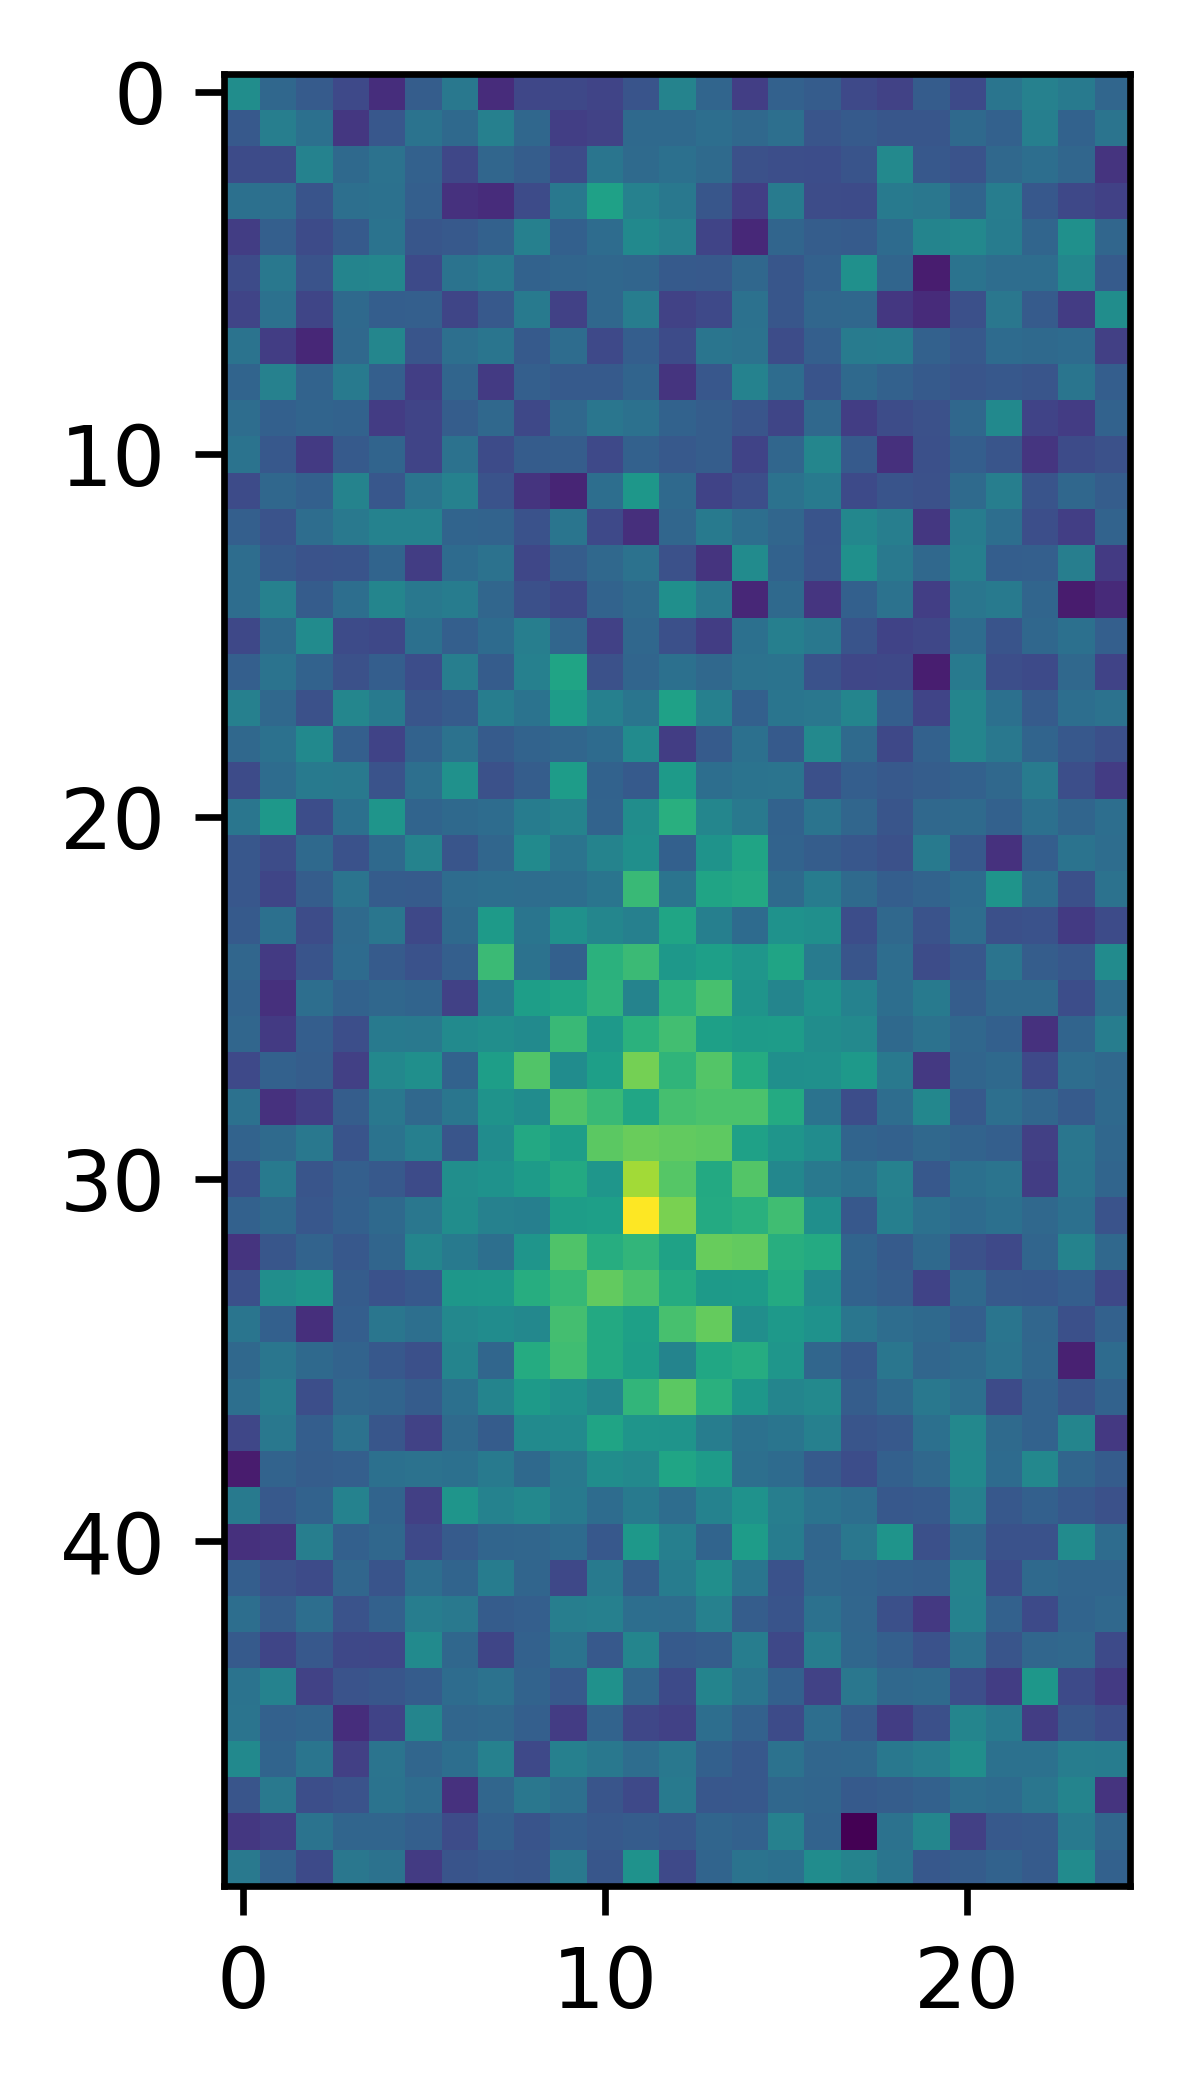
\includegraphics{Graphics/gaussian-2d-experiment3-row.png}}
	\subfigure[Por columnas]{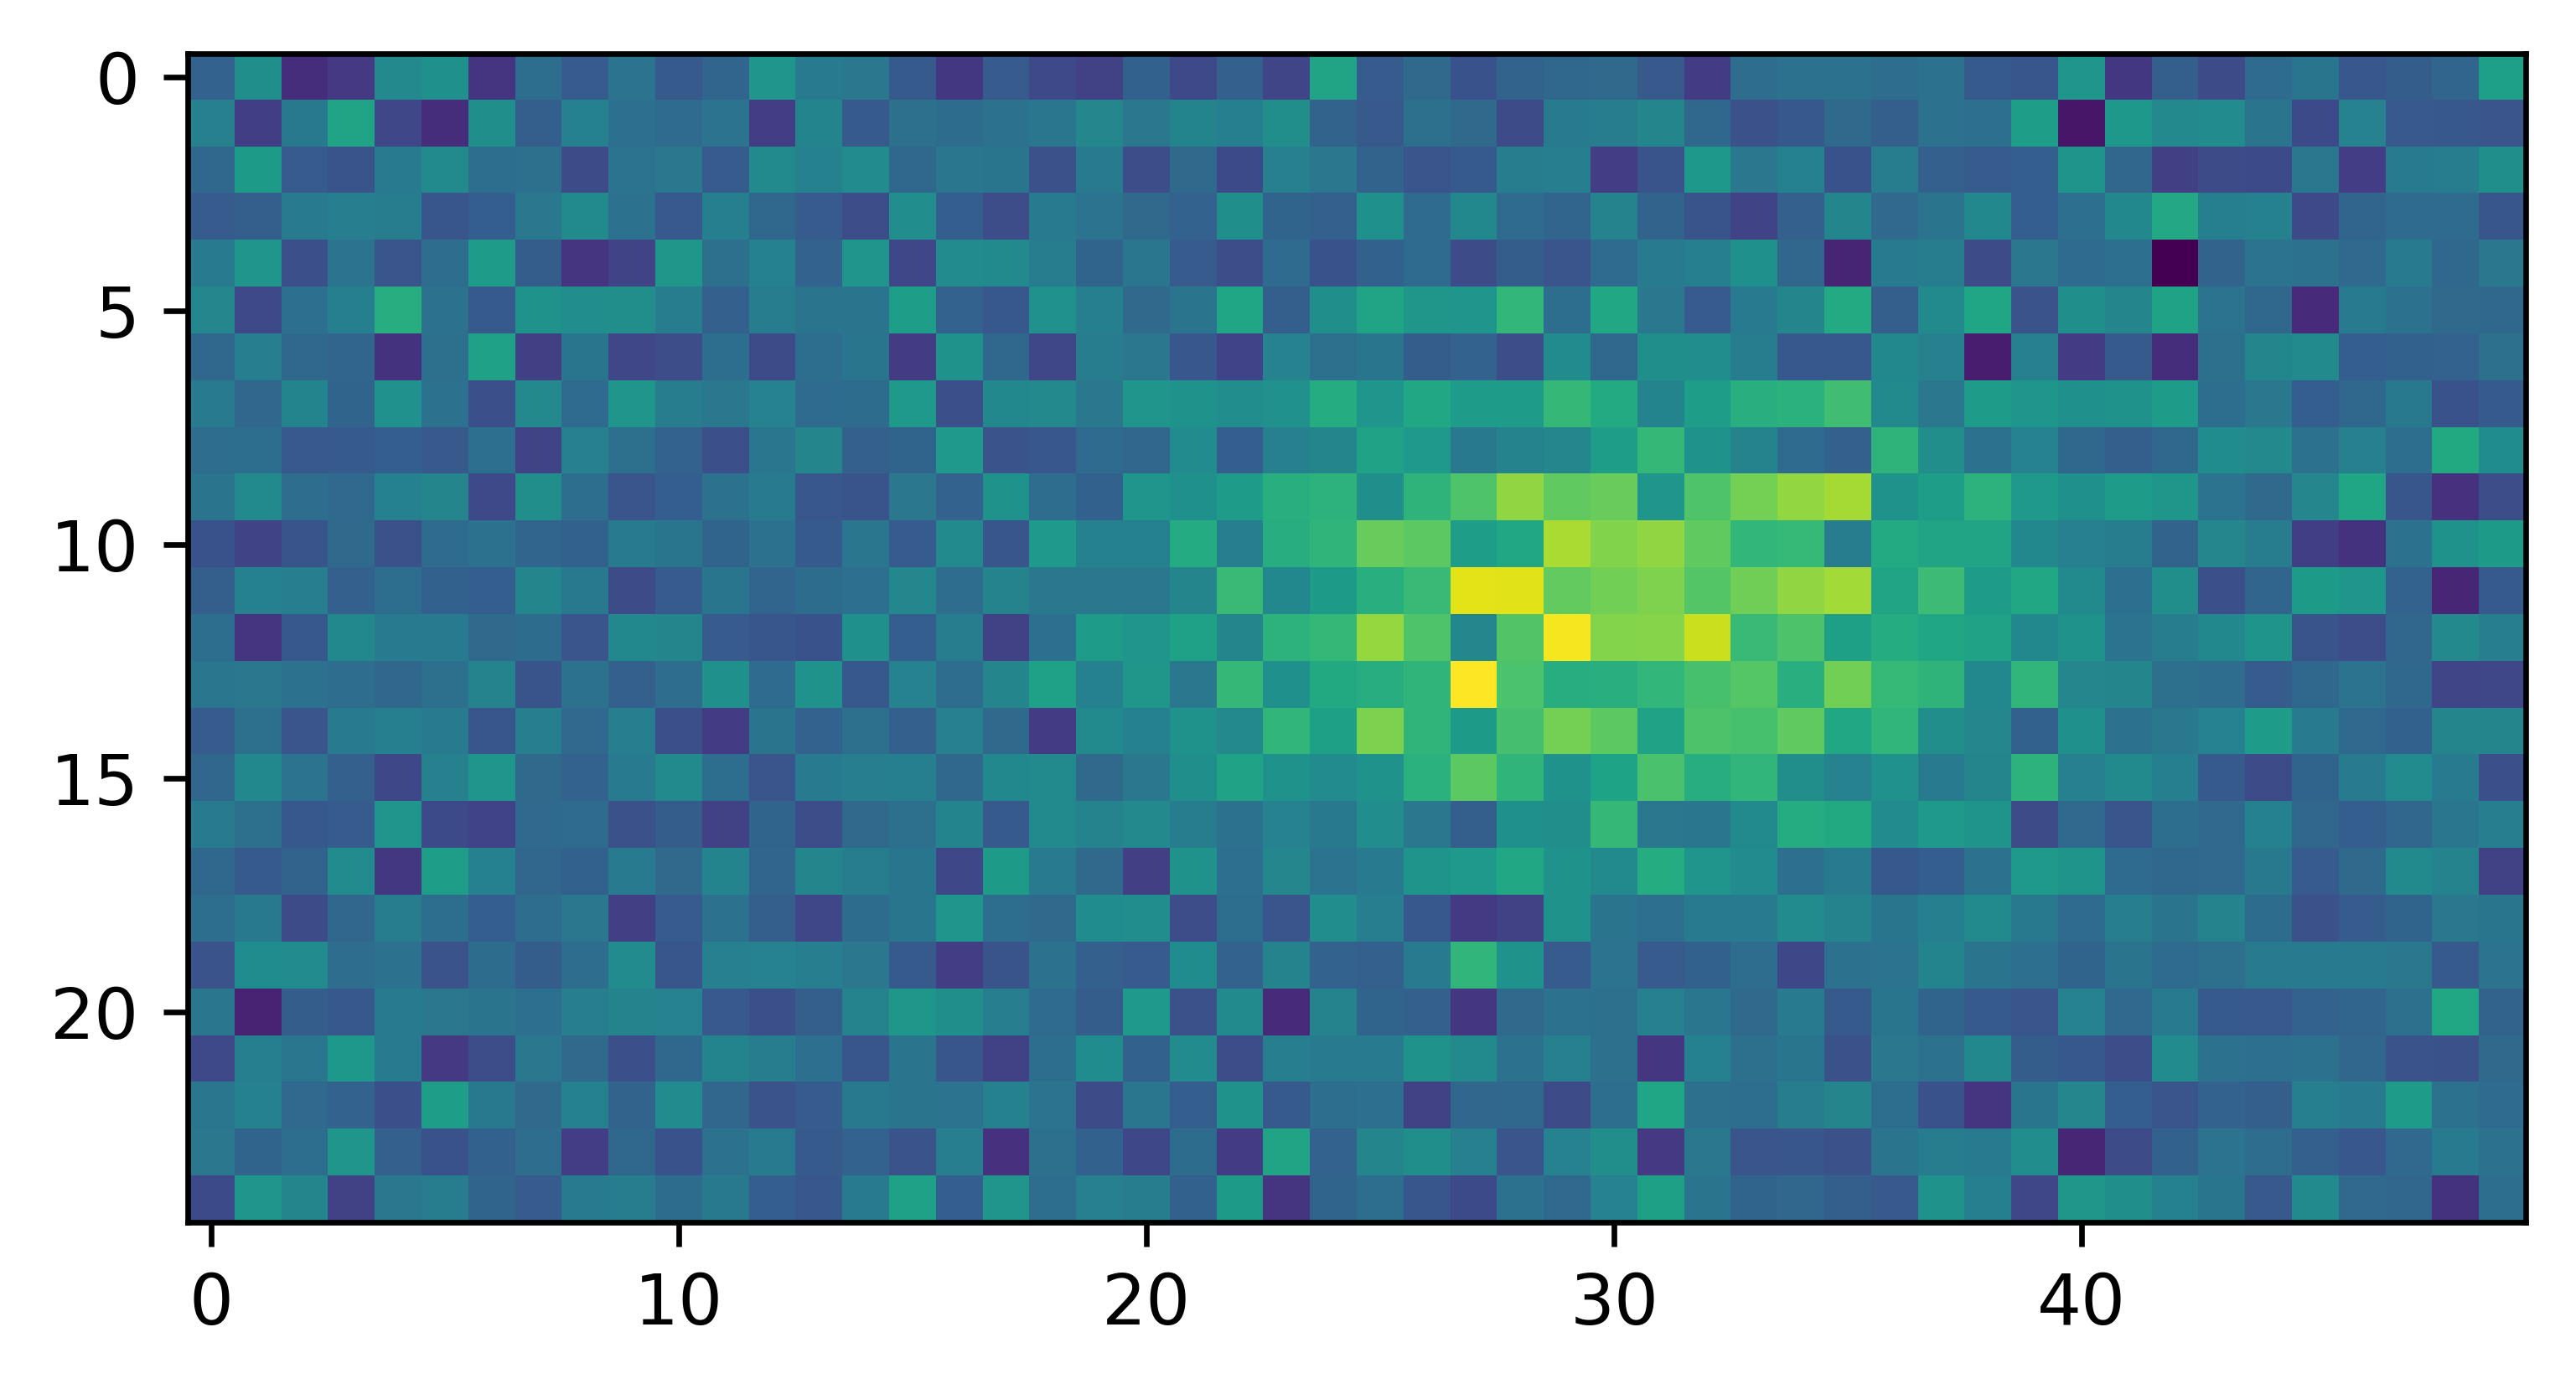
\includegraphics{Graphics/gaussian-2d-experiment3-col.png}}
	\caption{Resultado de evaluar $\mathbb{S}$ sobre cada una de las \textit{second-rated} de la DST-II usando el tercer enfoque.} \label{fig:gaussian-example-approach3}
\end{figure}

\section{Aplicación en la detección de masas en mamografías}

Para evaluar la capacidad del algoritmo de la DST-II y las propuestas de extensión al caso bidimensional en
la detección de masas de mamografías se usó la base de datos INBreast \cite{Moreira2012}. La misma 
contiene un total de 115 casos (410 imágenes), todas con anotaciones sobre distintos tipos de lesiones. 
En este caso, son de interés las de tipo masas, específicamente las que presentan isotropía.

Las imágenes poseen una resolución de $3328\times 4084$ o $2560\times 3328$ y están guardadas en formato
DICOM. Para su lectura se usó el paquete Pydicom \cite{darcy_mason_2020_4313150}.

Dado que las imágenes tienen una resolución alta se realiza un pre-procesamiento antes de aplicar el
algoritmo. Como primer paso, se realiza un reescalado de las imágenes. Para esto se usa la función de scikit-image
\textit{skimage.transform.rescale} con un factor de $\frac{1}{8}$ \cite{skimage-transform}. Luego de este reescalado,
se realiza un suavizado a la imagen y un \textit{sharpening}. El primero se realiza con un filtro guassiano
para eliminar la existencia de ruido en la mamografía. Para el segundo se usa un filtro laplaciano con el objetivo
de detectar mejor los bordes. Ambos resultados se fusionan y sobre esa imagen se aplica el algoritmo.

A continuación se muestra un ejemplo de los experimentos realizados.

\subsection{Ejemplos de los experimentos y análisis de los resultados}

El ejemplo tomado se muestra en la Figura \ref{fig:example-mm}. La imagen muestra los resultados de cada etapa 
del preprocesamiento: reescalado, filtro gaussiano, filtro laplaciano y, por último, fusión de los
resultados de ambos filtros.

\begin{figure*}
	\begin{multicols}{2}
		\subfigure[Reescalado]{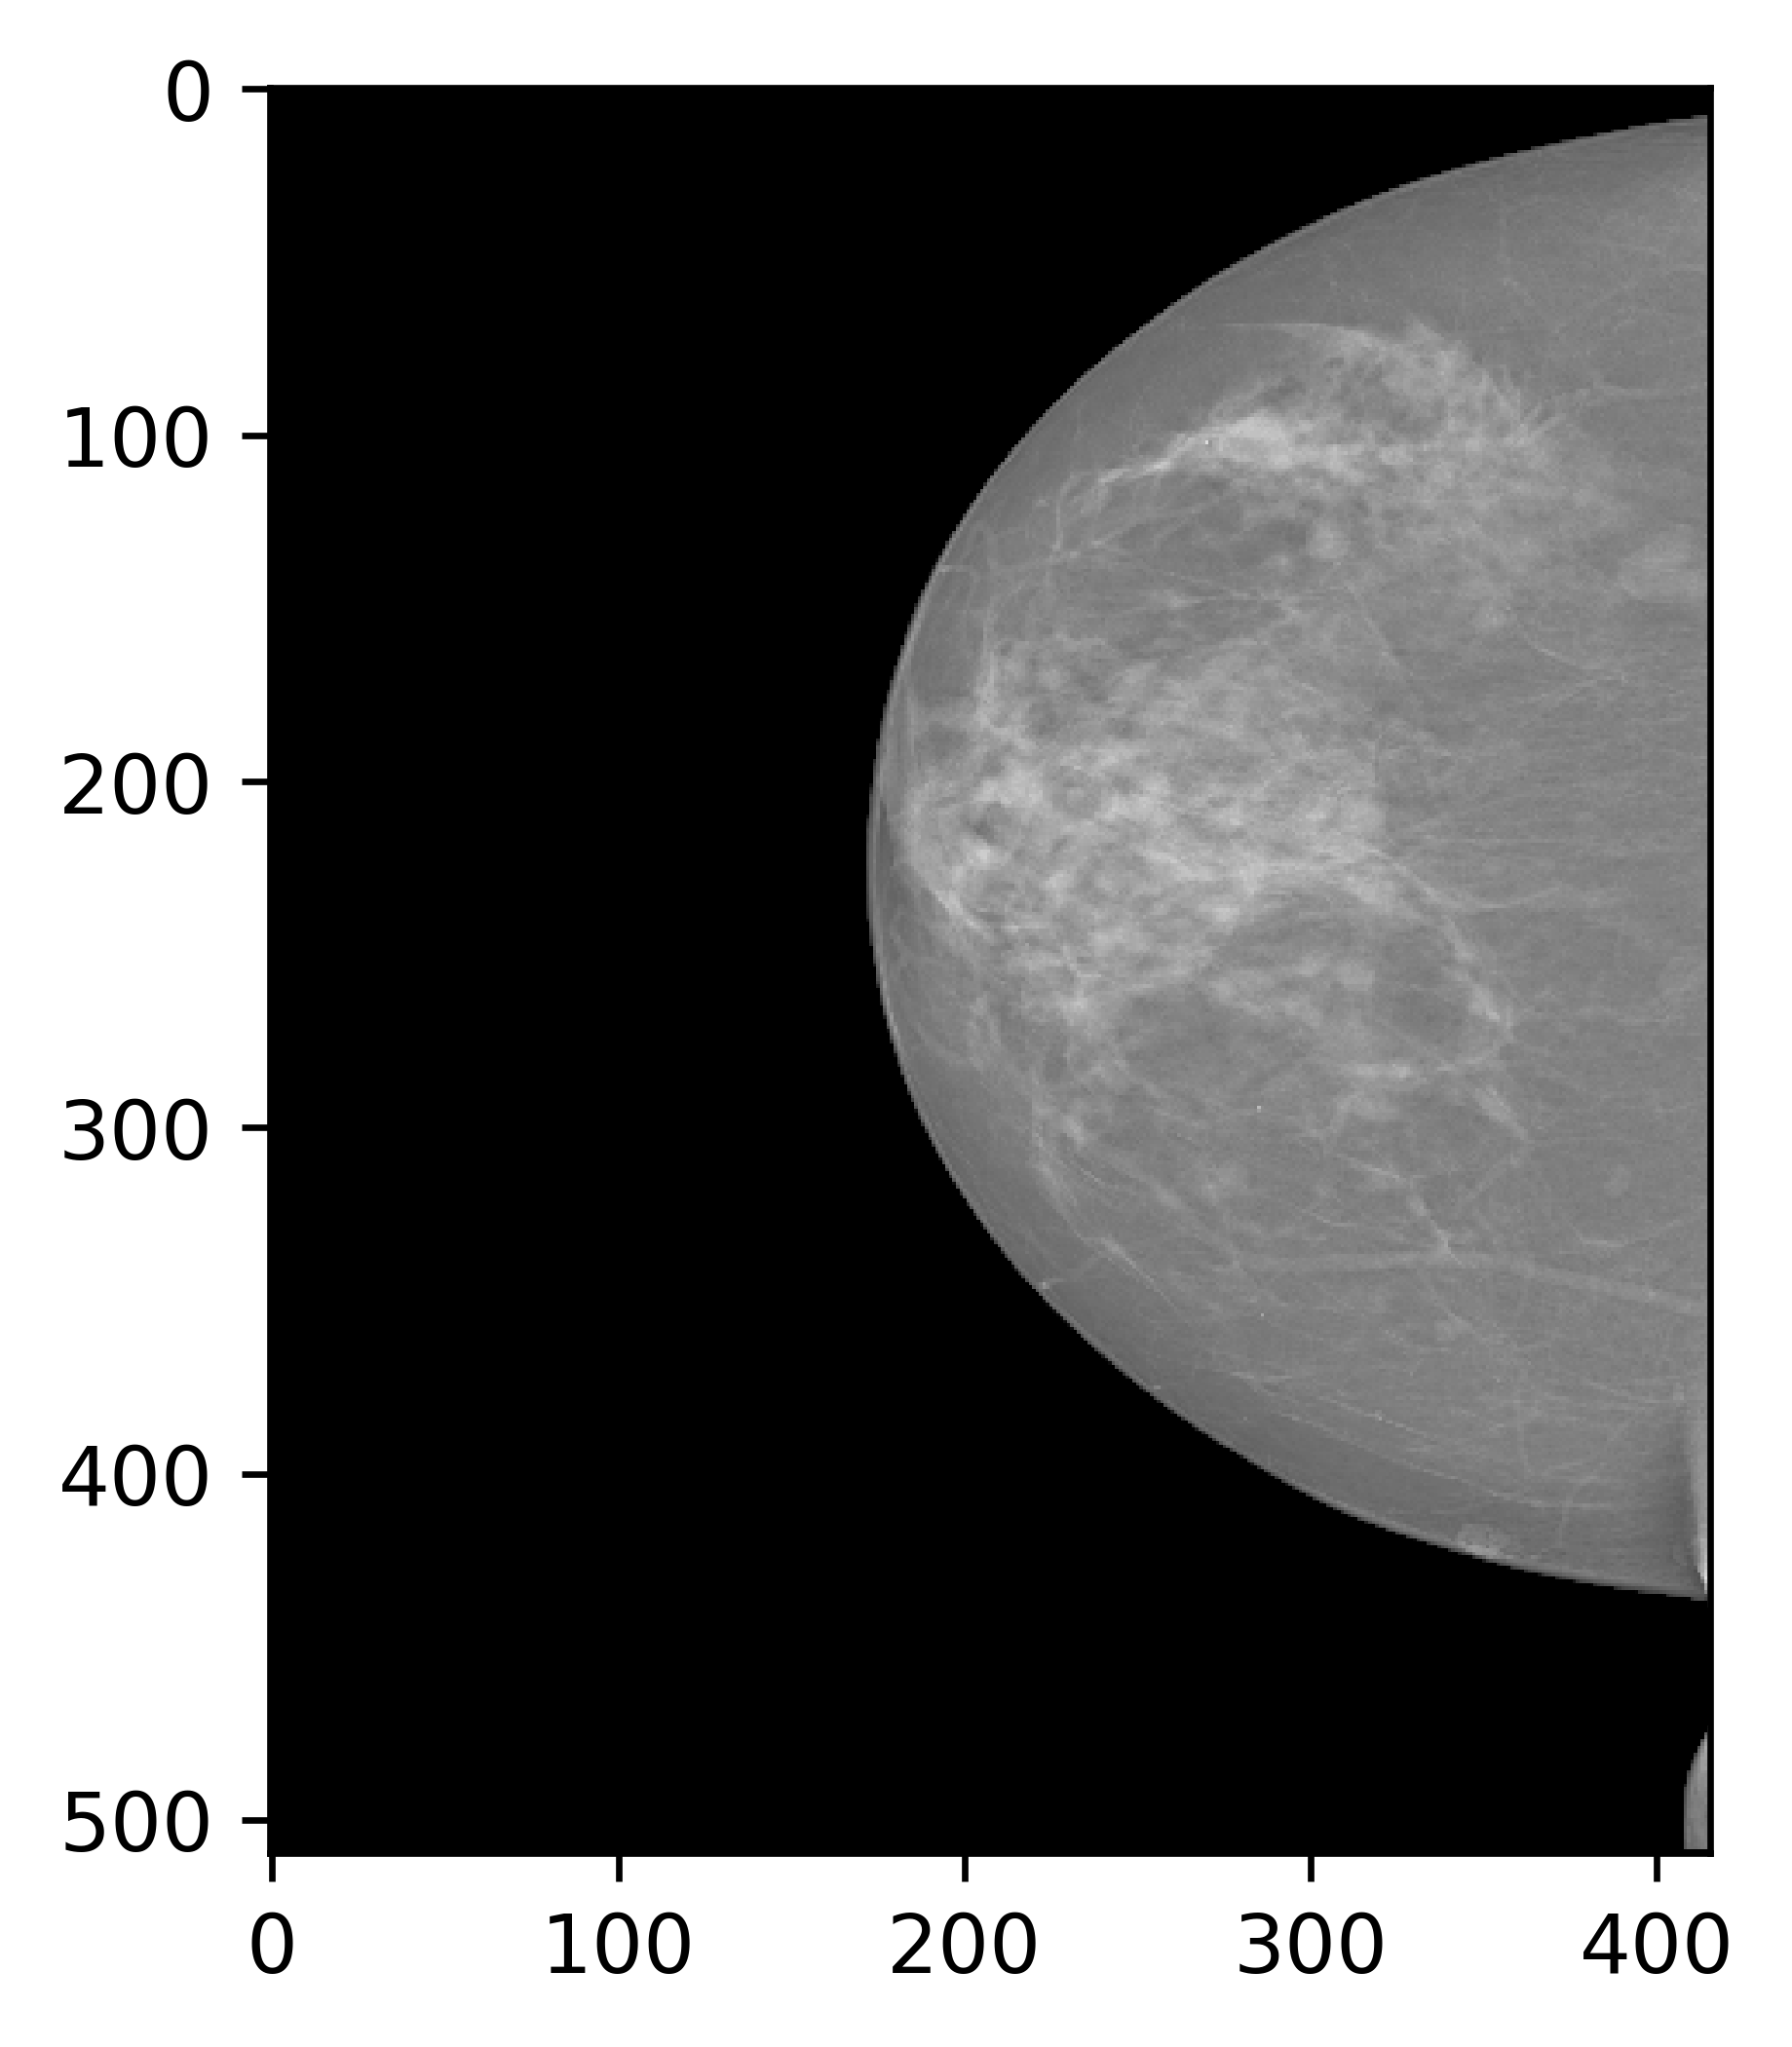
\includegraphics[scale=0.9]{Graphics/mm-rescaled.png}}\par
		\subfigure[Filtro gaussiano]{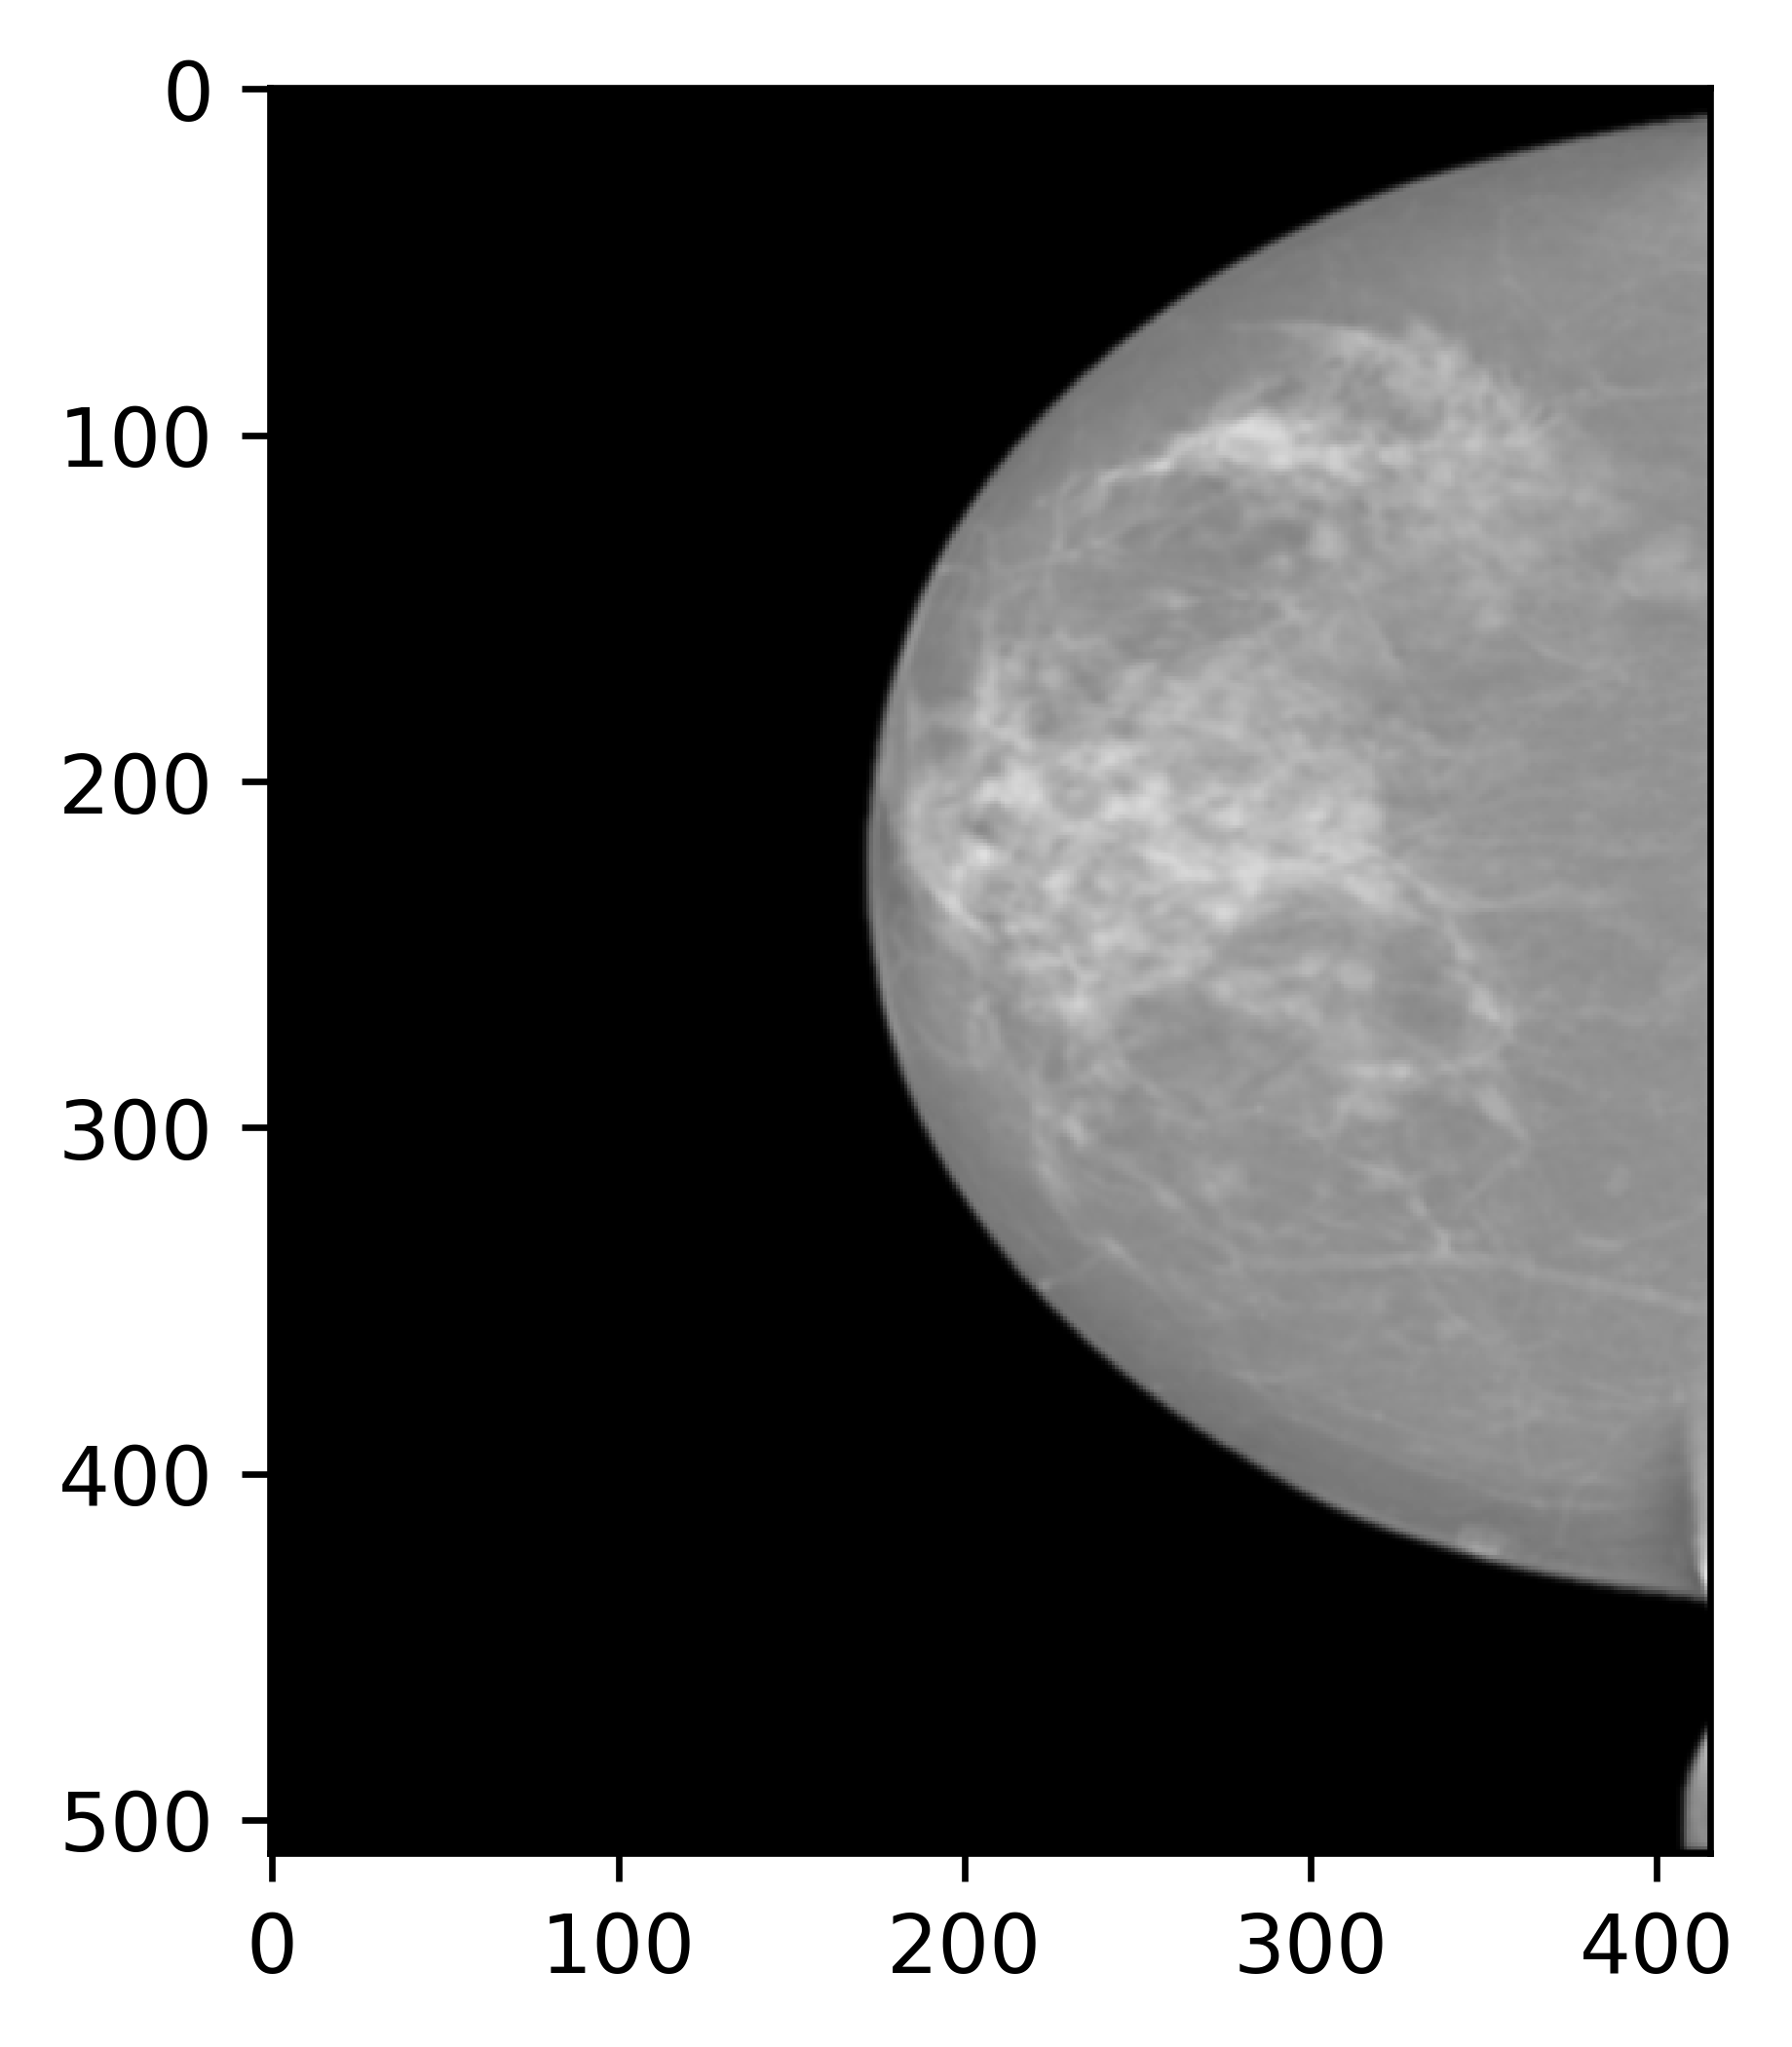
\includegraphics[scale=0.9]{Graphics/mm-smooth.png}}\par
		\end{multicols}
	\begin{multicols}{2}
		\subfigure[Filtro laplaciano]{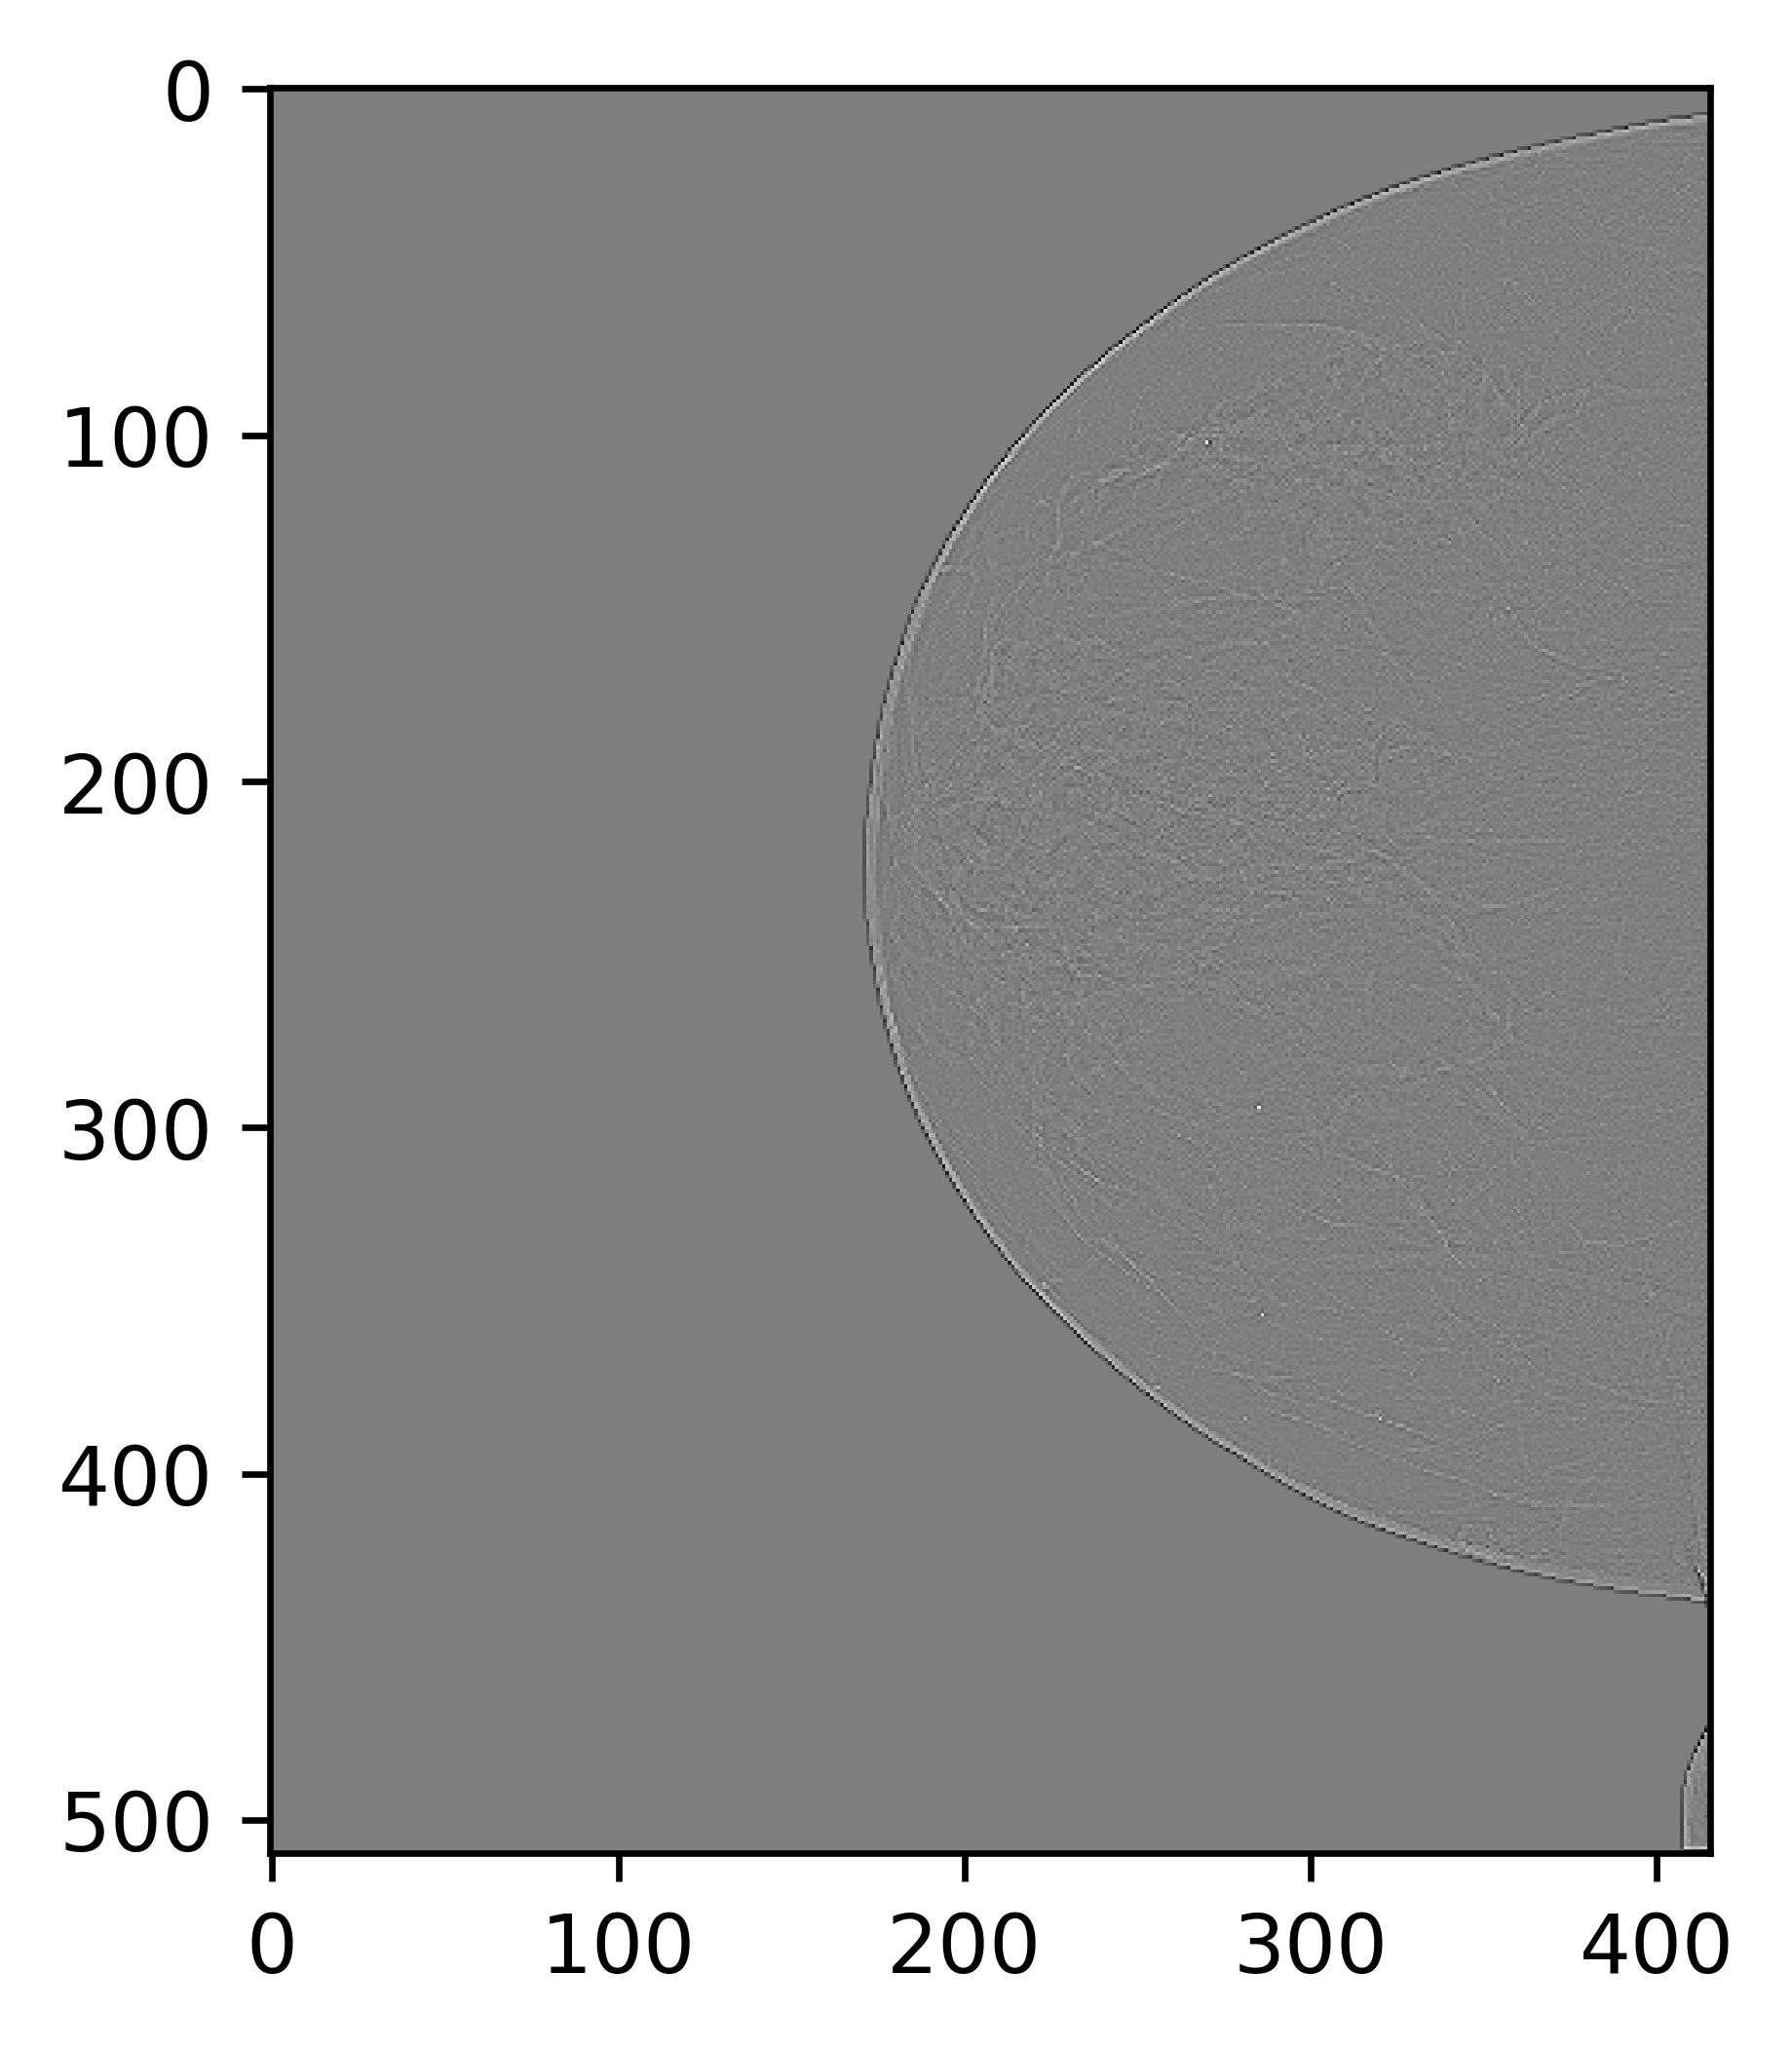
\includegraphics[scale=0.9]{Graphics/mm-sharp.png}}\par
		\subfigure[Fusión]{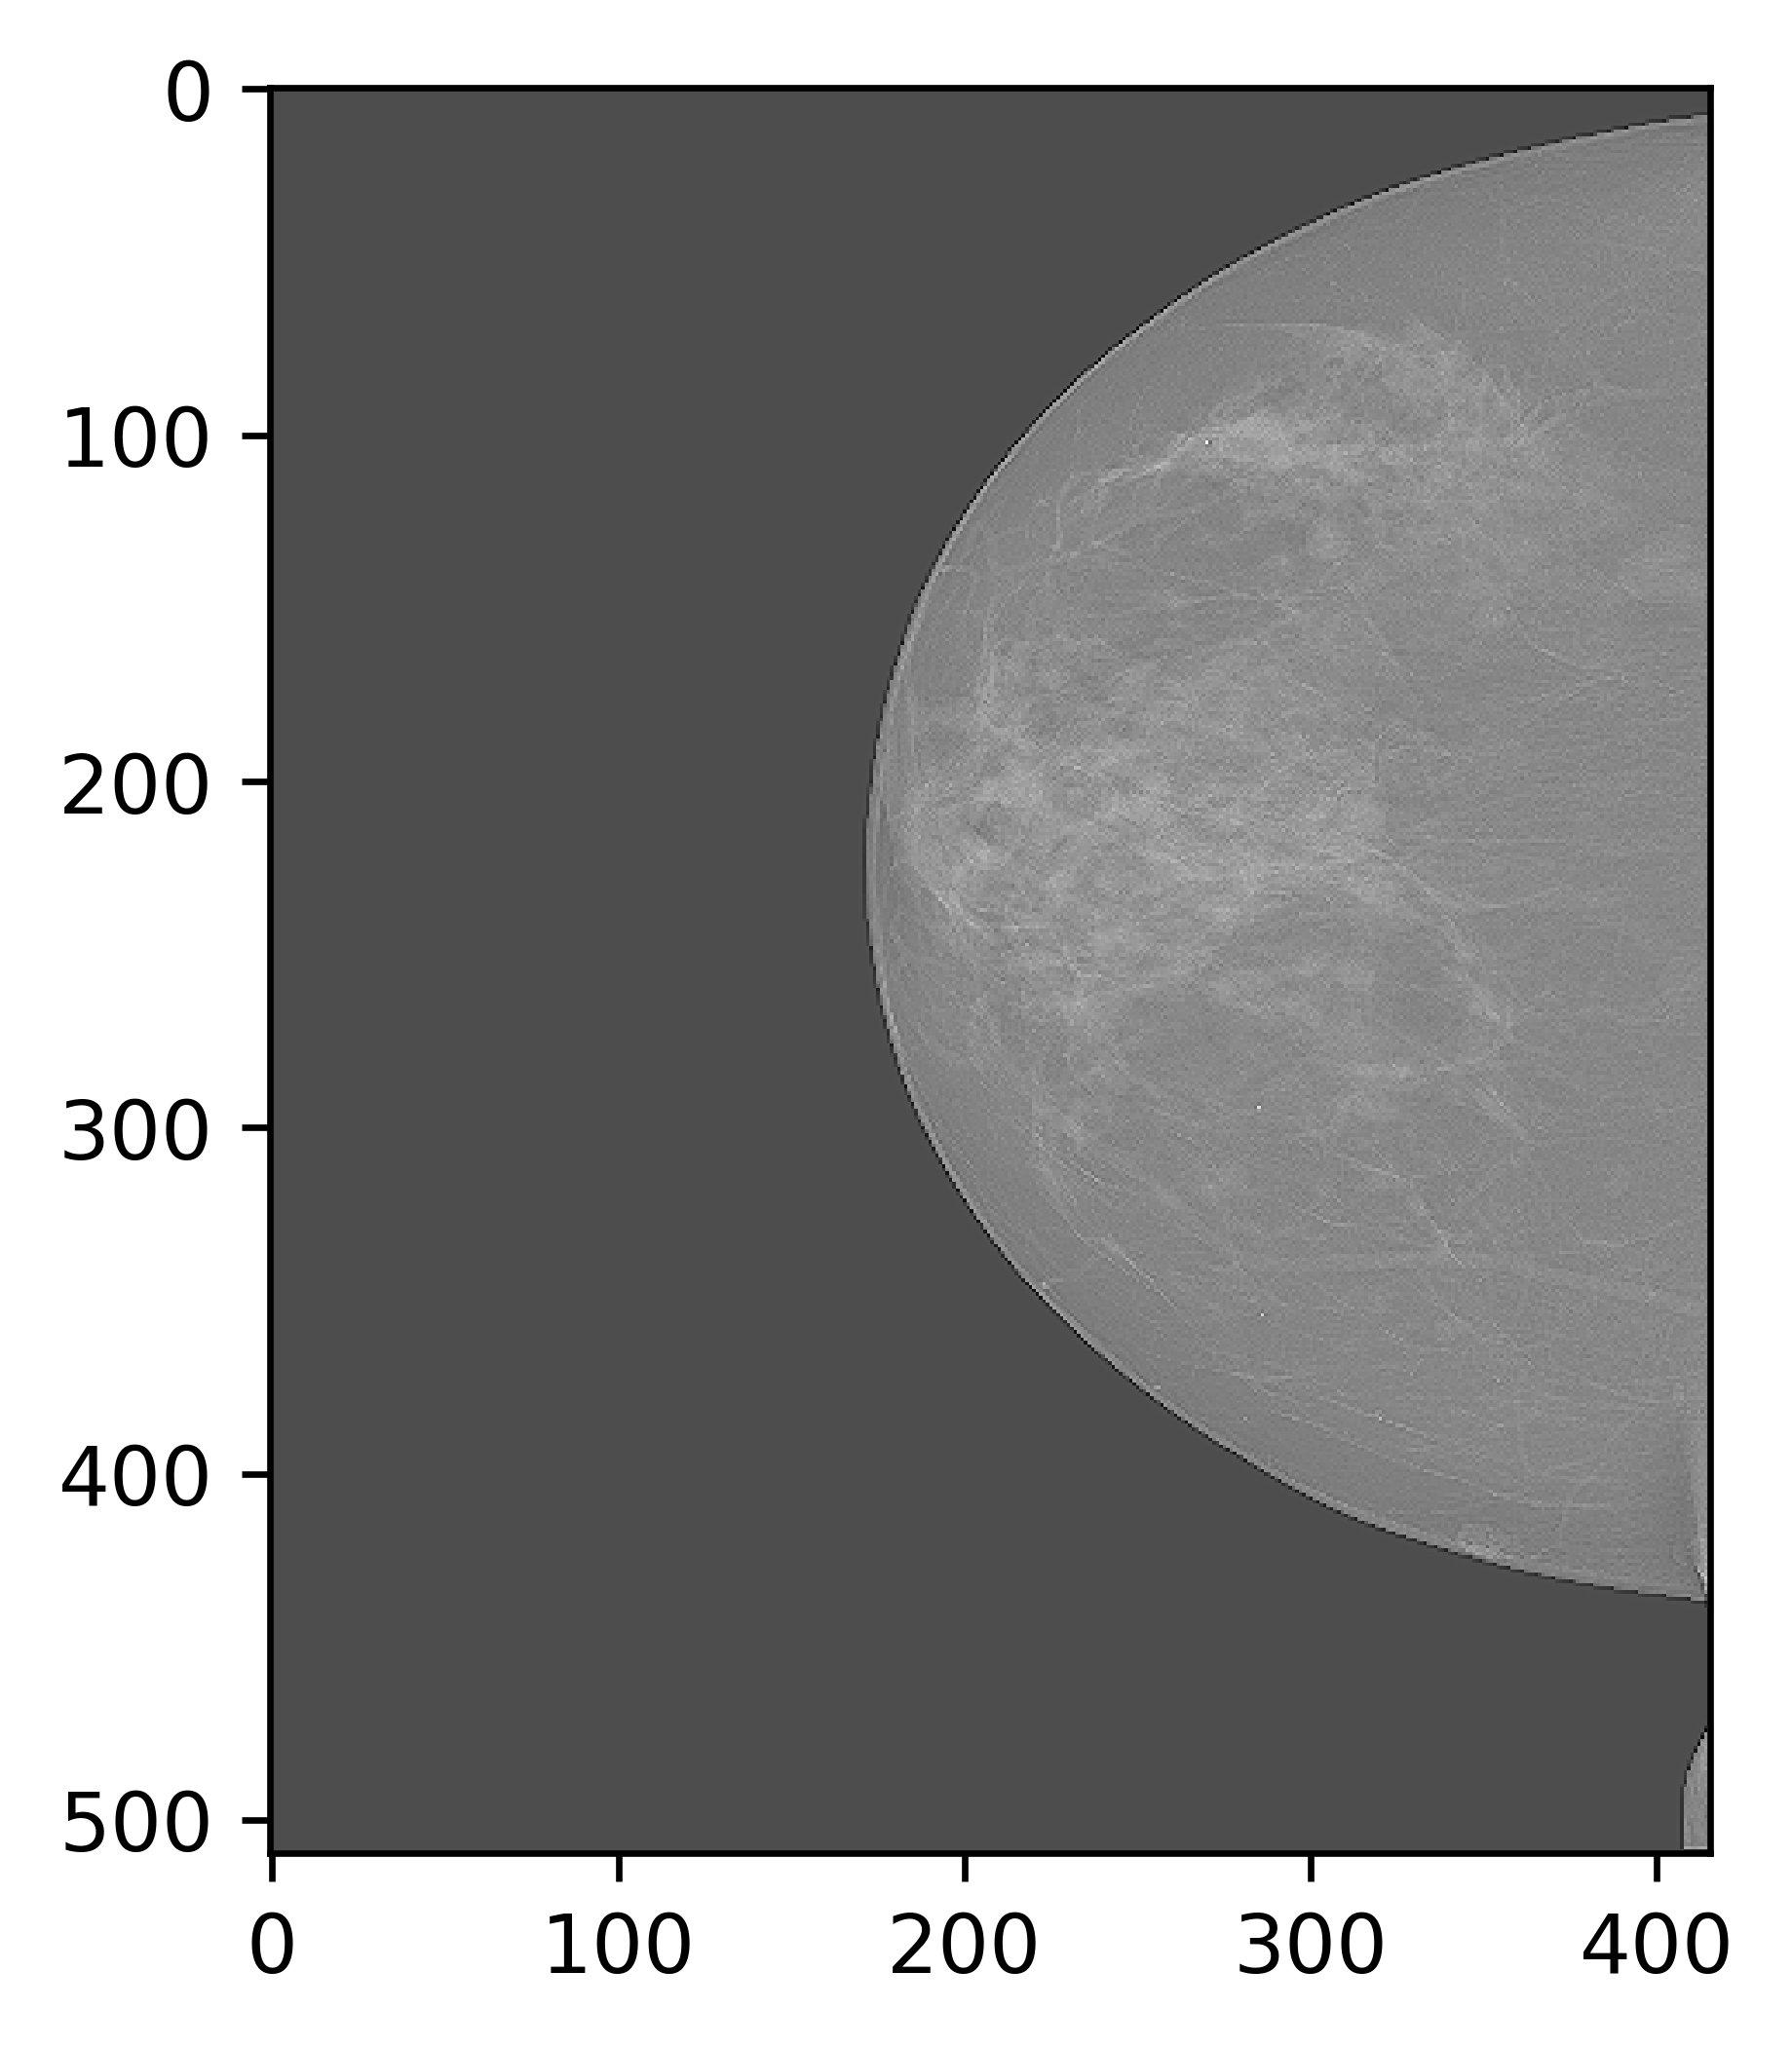
\includegraphics[scale=0.9]{Graphics/mm-fusion.png}}\par
	\end{multicols}
	\caption{Ejemplo de mamografía.} \label{fig:example-mm}
\end{figure*}


\begin{figure}
	\centering
	\subfigure[Masas]{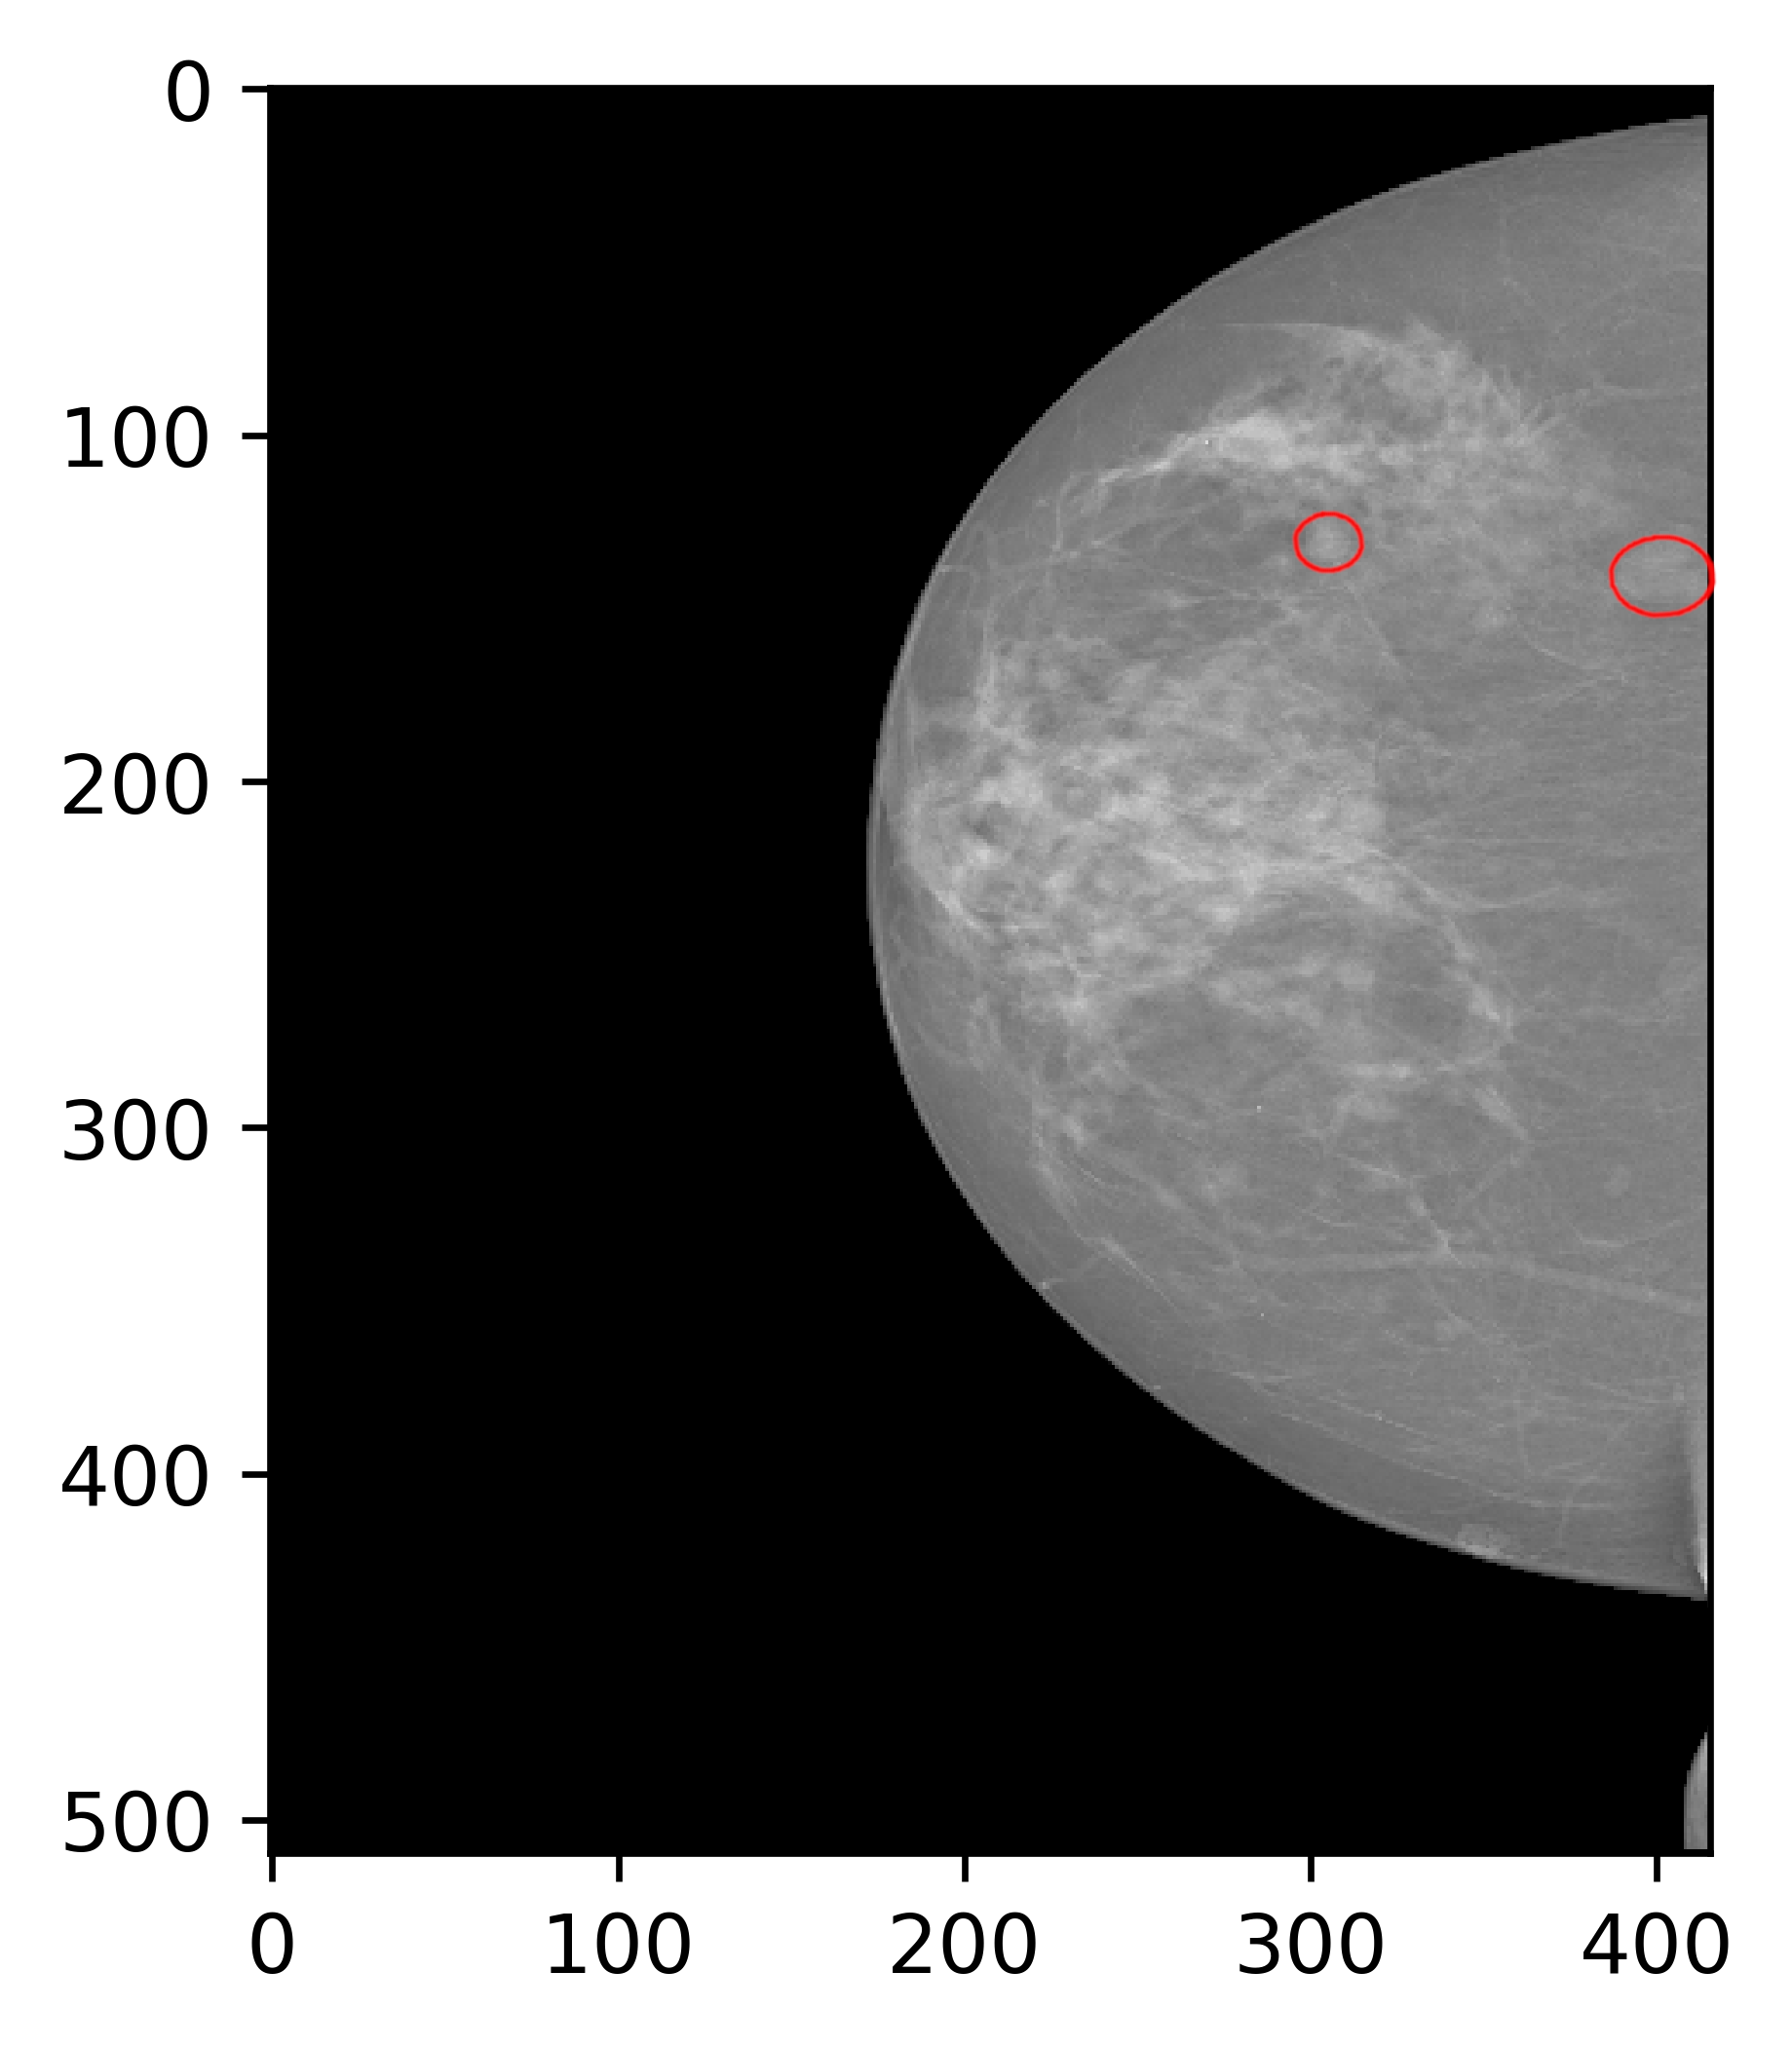
\includegraphics{Graphics/mm-rescaled-mass.png}}
	\subfigure[Porción de la mamografía donde se aplica el algoritmo]{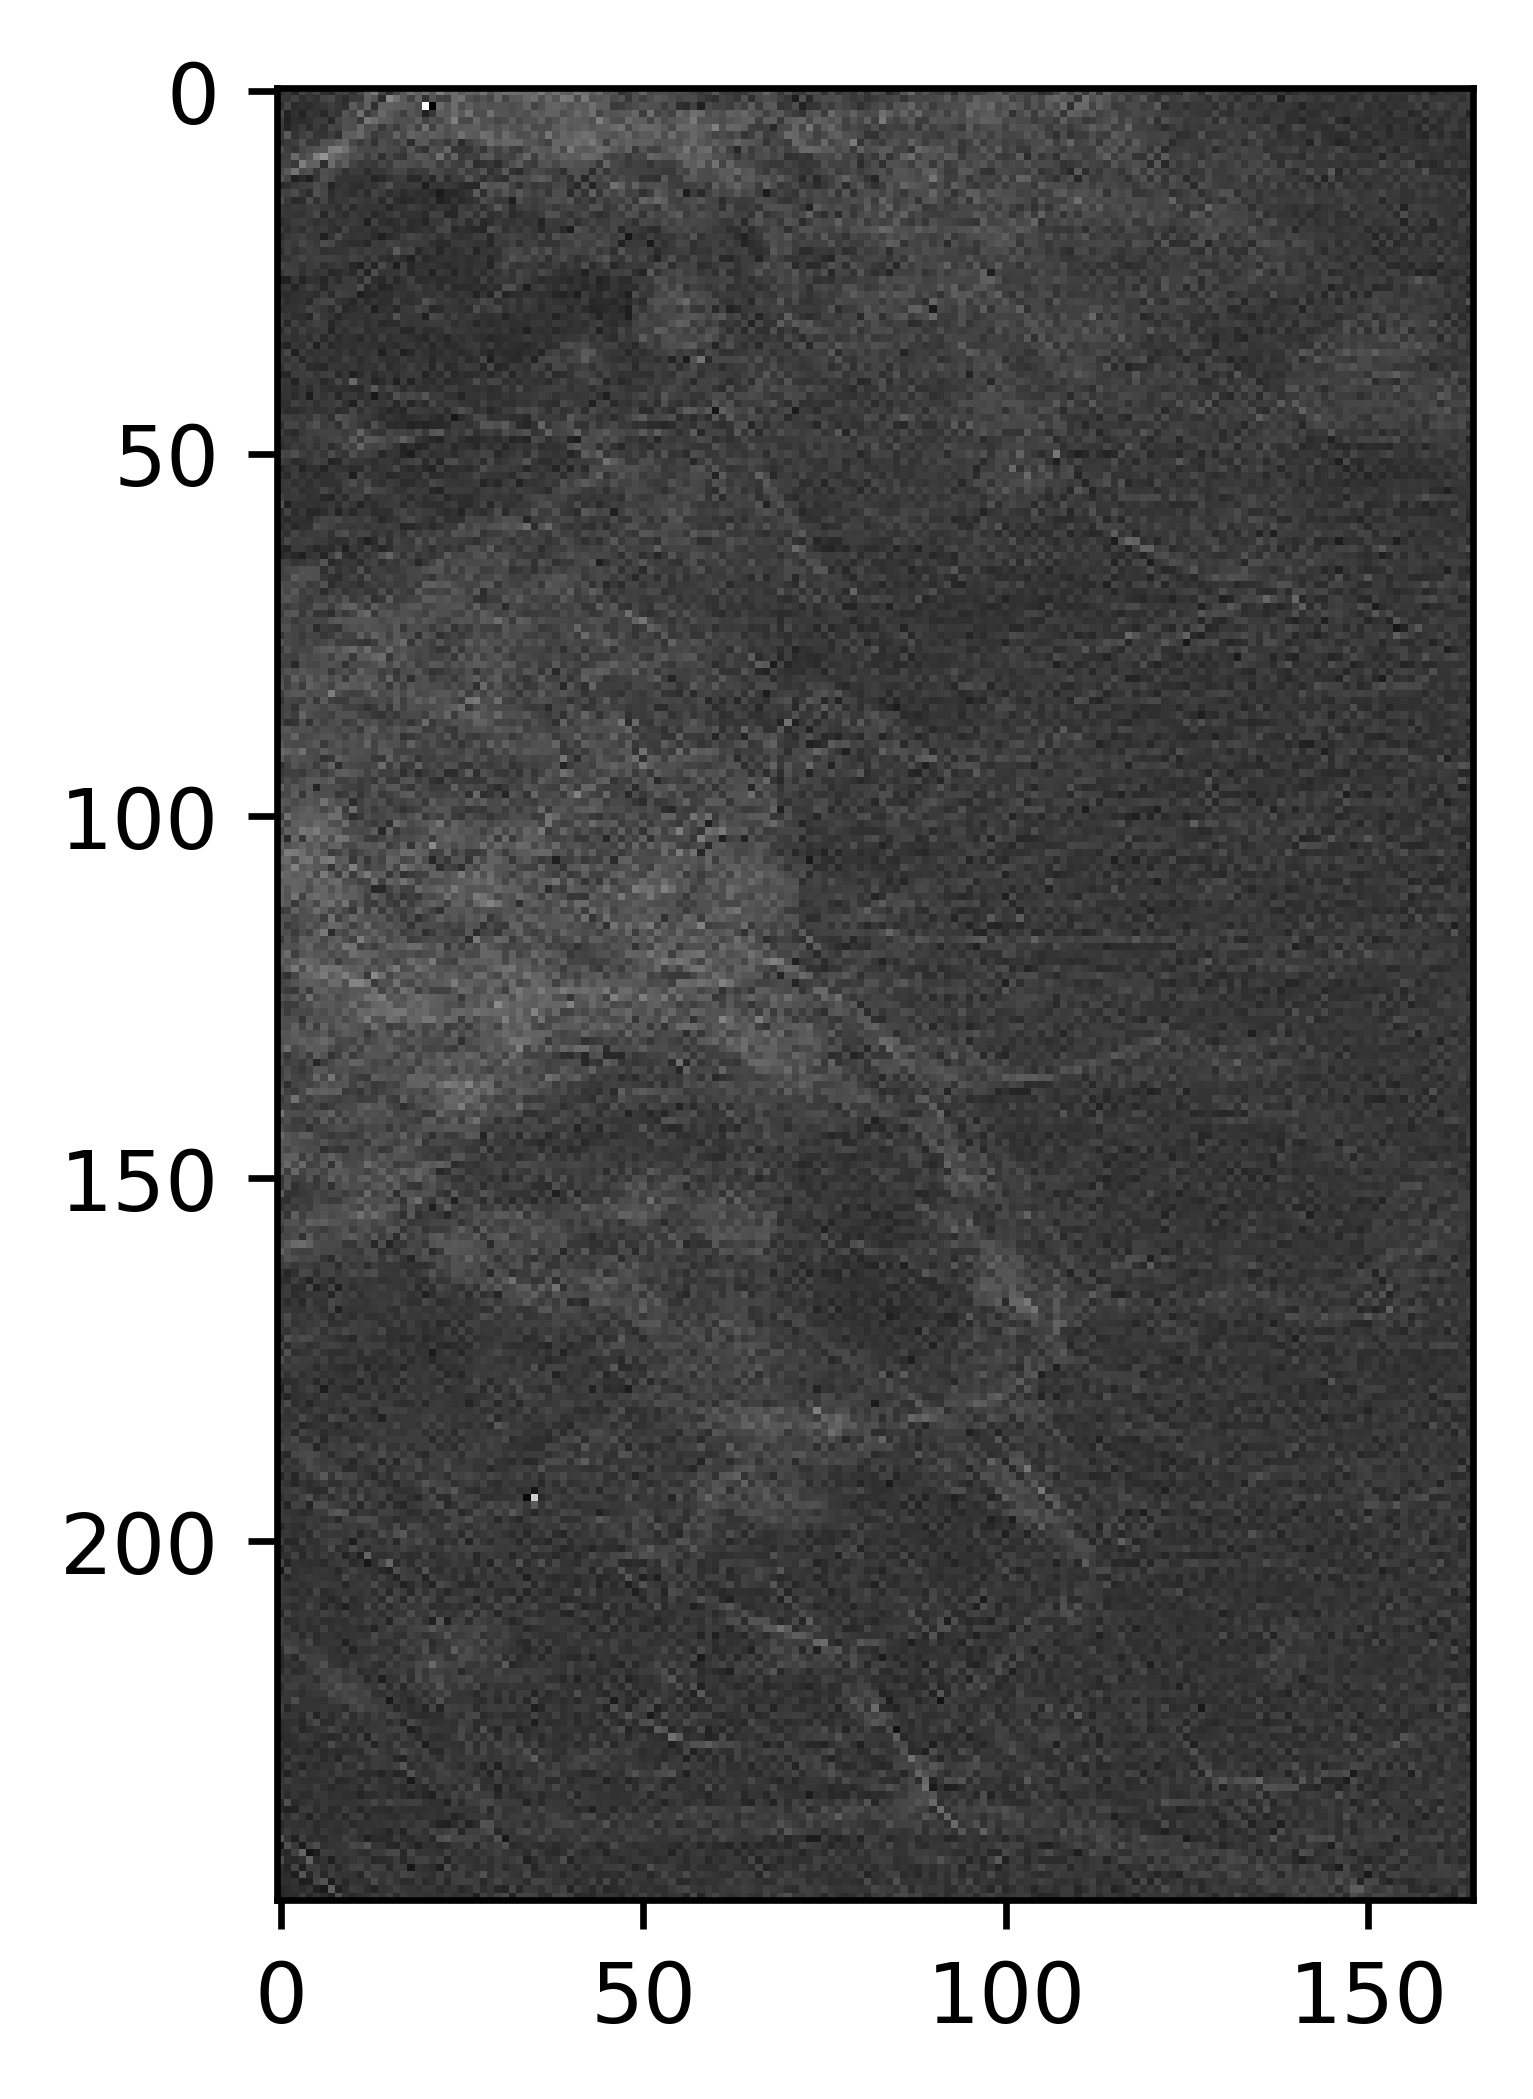
\includegraphics{Graphics/mm-portion.png}}
	\caption{Mamografía con la ubicacioón de las masas y la sección donde se aplica el algoritmo.} \label{fig:example-mm-portion}
\end{figure}

En la imagen de ejemplo existen dos masas. Pero solo se toma una para construir la(s) shapelet(s), de este modo 
se evalúa la capacidad del algoritmo para la detección de masas en general. En el caso ideal debería detectar ambas
regiones. Otro aspecto importante es que para el experimento se toma una sección de la mamografía donde no aparece 
el fondo negro, debido a que introduce muchos falsos positivos por el hecho de que los píxeles sean iguales a
cero. 

La Figura \ref{fig:example-mm-portion} muestra la ubicación de las masas y la porción de la mamografía sobre
la cual se realiza el algoritmo de detección. La primera de izquierda a derecha es la seleccionada para construir
la(s) shapelet(s).

\begin{figure*}
	\begin{center}
	\begin{multicols}{2}
		\subfigure[Coeficientes de aproximación]{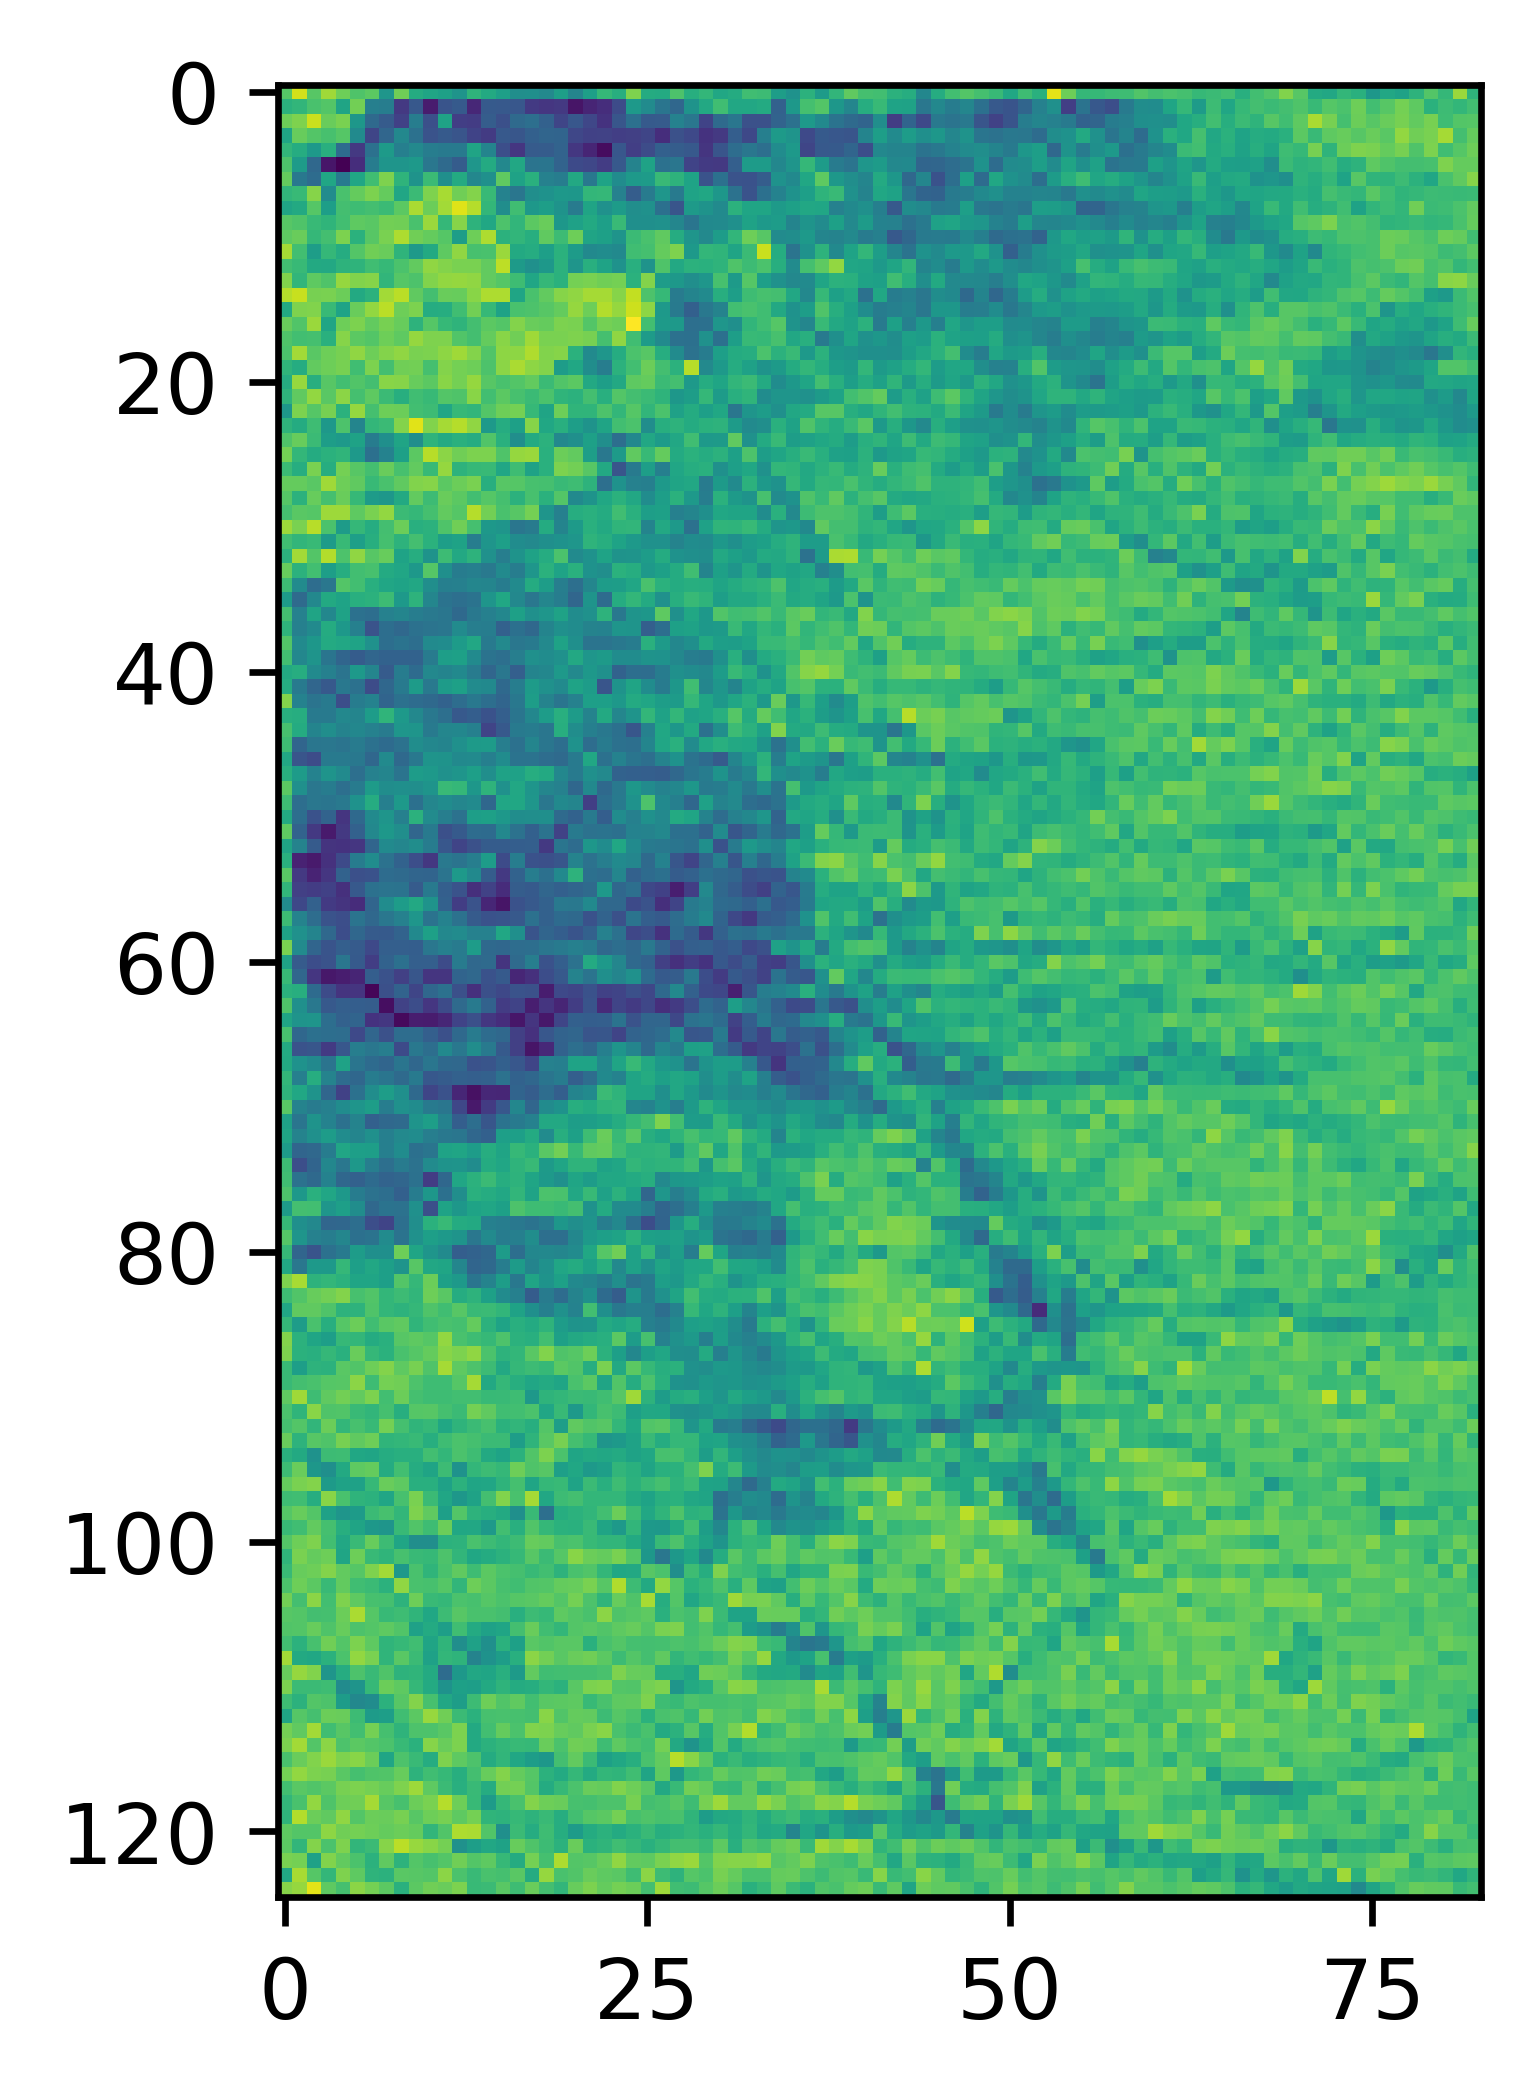
\includegraphics[scale=0.95]{Graphics/mm-aprox.png}}
		\subfigure[Coeficientes de detalle horizontal]{\includegraphics[scale=0.95]{Graphics/mm-horizontal.png}}
    \end{multicols}
	\begin{multicols}{2}
		\subfigure[Coeficientes de detalle vertical]{\includegraphics[scale=0.95]{Graphics/mm-vertical.png}}
		\subfigure[Coeficientes de detalle diagonal]{\includegraphics[scale=0.95]{Graphics/mm-diagonal.png}}
	\end{multicols}
	\end{center}
\caption{Resultado de la medida $\mathbb{S}$ sobre cada una de las cuatro componentes de la DST-II.} \label{fig:example-mm-approach1}
\end{figure*}

El resultado del primer enfoque se muestra en la Figura \ref{fig:example-mm-approach1}. Nótese que
tanto en este caso como en el
del ejemplo de la gaussiana, no hay ningún signo de detección. Esto refuerza aún más la conclusión de que la DST-II no se puede
extender para el caso 2D con este enfoque.

\begin{figure}
	\centering
	\subfigure[Por filas]{\includegraphics{Graphics/mm-row.png}}
	\subfigure[Por columnas]{\includegraphics{Graphics/mm-col.png}}
	\caption{Resultado de evaluar $\mathbb{S}$ sobre cada una de las \textit{second-rated} de la DST-II usando el segundo enfoque.} \label{fig:example-mm-approach2}
\end{figure}
%Detection at position (32, 27) with value 0.9831863519468129 row
%Detection at position (14, 59) with value 0.983604207430764 col

En el caso del segundo enfoque, los resultados son mejores. Si se observa la Figura \ref{fig:example-mm-approach2}, al menos hay signos de detección.
Aunque bien difíciles de ver, existen un par de píxeles (de color amarillo), uno en cada imagen que constrastan con el resto.
Estos están ubicados en las posiciones $(32,27)$ y $(14,59)$ con valores $\mathbb{S}=0.9831863519468129$ y $\mathbb{S}=0.983604207430764$,
respectivamente. Ambos corresponden a las posiciones aproximadas $(32,54)$ y $(28,59)$, que es donde se encuentra el patrón extraído.
La Figura \ref{fig:example-mm-approach3} muestra la mamografía con las posiciones 
predichas por el algoritmo basado en $\mathbb{S}$. Los píxeles de color rojo indican estas posiciones.
A pesar de que el segundo enfoque logra detectar la posición donde se encuentra el patrón con el cual se construyeron
las \textit{shapelets}, no detecta la segunda masa.

\begin{figure}
	\centering
	\subfigure[Por filas]{\includegraphics{Graphics/mm-multi-row.png}}
	\subfigure[Por columnas]{\includegraphics{Graphics/mm-multi-col.png}}
	\caption{Resultado de evaluar $\mathbb{S}$ sobre cada una de las \textit{second-rated} de la DST-II usando el tercer enfoque.} \label{fig:example-mm-approach3}
\end{figure}


\begin{figure}
	\centering
	\includegraphics{Graphics/mm-detection-s-on-mm.png}
	\caption{Mamografía con las posiciones predichas por el algoritmo basado en $\mathbb{S}$. Dentro del círculo de color rojo se encuentran dos píxeles que indican estas posiciones.} \label{fig:mm-approach2-mm-s}
\end{figure}

El tercer enfoque no logra buenos resultados, tal y como se muestra en la Figura \ref{fig:example-mm-approach3}.
No se logra ningún signo de detección y, de hecho, los valores no superan $\mathbb{S}=0.8$. 

Como conclusión general de los experimentos, se puede decir que se logró una replicación exitosa de la DST-II,
y que en el caso unidimensional funciona adecuadamente como clasificador para la presencia de un patrón 
dentro de una señal. Sin embargo, una desventaja es el tamaño del patrón. Mientras mayor cantidad
de muestras contenga más díficil es resolver el sistema de ecuaciones no lineales y si el error de la
solución es alto no se logra detección. 
En el caso 2D, ninguno de los enfoques usados para extender este algoritmo al caso
bidimensional fue fructífero. Aunque el segundo enfoque logró hacer detecciones, solo es capaz
de identificar la posición del patrón a través de un único píxel y no sobre una región o
contorno. Esto complica la capacidad de visualizar
dicha detección. Por último, otro aspecto importante es la sensibilidad ante el ruido del algoritmo. 
Aunque la DST-II logre detectar el patrón, modificaciones del mismo son díficiles de detectar.
En el caso de las masas, sus diversos tamaños y formas, no permiten que el algoritmo sea capaz de detectarlas
a partir de un único patrón.



\backmatter

\begin{conclusions}
	En este trabajo se replicó el algoritmo de la DST-II para la detección de patrones en 
	señales unidimensionales
	y se exploraron vías para la extensión del mismo al caso bidimensional, aplicando 
	estas propuestas en señales artificiales y en la detección de masas en mamografías.
	
	La replicación del algoritmo logró encontrar un error en la definición de las ecuaciones de detección 
	en el artículo original, provocando un cambio en dichas condiciones. Teniendo en cuenta esto último, se puede
	decir que se logró replicar el algoritmo exitosamente. 
	Se compararon distintos métodos de optimización para solucionar el sistema de ecuaciones no lineales, y
	se obtuvo que los más eficaces son el método de Levenberg-Marquardt y el método híbrido de Powell.

	También se encontraron deficiencias en el
	algoritmo de la DST-II. Se comprobó que el resultado de la transformada en la detección 
	de patrones depende en gran medida
	de la calidad de la solución numérica encontrada. Si el error es alto, no se logra una diferencia marcada
	entre el punto donde se encuentra el patrón y el resto. De los métodos probados, cuando el sistema contaba
	con más de 24 variables, la mayoría de las veces no se alcanzó la convergencia, lo que influyó 
	directamente en la capacidad del algoritmo para detectar el patrón. Otra deficiencia encontrada del 
	algoritmo es su sensibilidad ante el ruido, es decir, solo es capaz de detectar al patrón exacto con el cual 
	se diseñó la \textit{shapelet}. Esto es consecuencia de las condiciones de detección, que son muy estrictas.

	En el caso 2D, se exploró tres alternativas. Se evaluaron las mismas en señales artificiales que incluyen
	gaussianas, círculos y regiones rectangulares en distintas configuraciones. Se logró identificar
	las deficiencias de cada una de estas alternativas. También se usaron y evaluaron las tres
	propuestas en la detección de anomalías de tipo masa en mamografías.
	 
	Por último, la principal conclusión de esta tesis es que debido a las características del algoritmo (sobretodo las 
	condiciones de detección) 
	no se pudo extender exitosamente al caso 2D mediante las tres alternativas, como sí sucede con otras wavelets. 
	Ninguna de las propuestas mostradas aquí
	resultó ser eficaz, ni para señales artificiales ni para la detección de masas en mamografías.

\end{conclusions}

\begin{recomendations}
	A pesar de que en este trabajo no se logró extender la DST-II para el caso bidimensional con enfoques 
	que funcionan con otras wavelets, se pueden explorar otras ideas.
	Se propone usar ideas similares a las de ecuaciones de detección, pero teniendo
	en cuenta la forma en que se hace la transformada en el caso 2D.

	A pesar de que la capacidad de detectar patrones de la DST-II tiene sus limitaciones, se puede explorar el uso
	de dicha transformada para la extracción de características para ser usados posteriormente por algoritmos
	de aprendizaje automático, y comparar resultados con otras wavelets.
\end{recomendations}

\include{BackMatter/Bibliography}

\end{document}
